%======================================================================
% University of Waterloo Thesis Template for LaTeX 
% Last Updated August 2023
% by IST Client Services, 
% University of Waterloo, 200 University Ave. W., Waterloo, Ontario, Canada
% FOR ASSISTANCE, please send mail to ist-helpdesk@uwaterloo.ca

% DISCLAIMER
% To the best of our knowledge, this template satisfies the current uWaterloo thesis requirements.
% However, it is your responsibility to assure that you have met all requirements of the University and your particular department.

% Many thanks for the feedback from many graduates who assisted the development of this template.
% Also note that there are explanatory comments and tips throughout this template.
%======================================================================
% Some important notes on using this template and making it your own...

% The University of Waterloo has required electronic thesis submission since October 2006. 
% See the uWaterloo thesis regulations at
% https://uwaterloo.ca/graduate-studies/thesis.
% This thesis template is geared towards generating a PDF version optimized for viewing on an electronic display, including hyperlinks within the PDF.

% DON'T FORGET TO ADD YOUR OWN NAME AND TITLE in the "hyperref" package configuration below. 
% Search for: PDFTITLE, PDFAUTHOR, PDFSUBJECT, and PDFKEYWORDS.
% THIS INFORMATION GETS EMBEDDED IN THE FINAL PDF DOCUMENT.
% You can view the information if you view properties of the PDF document.

% Many faculties/departments also require one or more printed copies. 
% This template attempts to satisfy both types of output. 
% See additional notes below.
% It is based on the standard "book" document class which provides all necessary sectioning structures and allows multi-part theses.

% If you are using this template in Overleaf (cloud-based collaboration service), then it is automatically processed and previewed for you as you edit.

% For people who prefer to install their own LaTeX distributions on their own computers, and process the source files manually, the following notes provide the sequence of tasks:
 
% E.g. to process a thesis called "mythesis.tex" based on this template, run:

% pdflatex mythesis	-- first pass of the pdflatex processor
% bibtex mythesis	-- generates bibliography from .bib data file(s)
% makeindex         -- should be run only if an index is used 
% pdflatex mythesis	-- fixes numbering in cross-references, bibliographic references, glossaries, index, etc.
% pdflatex mythesis	-- it takes a couple of passes to completely process all cross-references

% If you use the recommended LaTeX editor, Texmaker, you would open the mythesis.tex file, then click the PDFLaTeX button. Then run BibTeX (under the Tools menu).
% Then click the PDFLaTeX button two more times. 
% If you have an index as well,you'll need to run MakeIndex from the Tools menu as well, before running pdflatex
% the last two times.

% N.B. The "pdftex" program allows graphics in the following formats to be included with the "\includegraphics" command: PNG, PDF, JPEG, TIFF
% Tip: Generate your figures and photos in the size you want them to appear in your thesis, rather than scaling them with \includegraphics options.
% Tip: Any drawings you do should be in scalable vector graphic formats: SVG, PNG, WMF, EPS and then converted to PNG or PDF, so they are scalable in the final PDF as well.
% Tip: Photographs should be cropped and compressed so as not to be too large.

% To create a PDF output that is optimized for double-sided printing: 
% 1) comment-out the \documentclass statement in the preamble below, and un-comment the second \documentclass line.
% 2) change the value assigned below to the boolean variable "PrintVersion" from " false" to "true".

%======================================================================
%   D O C U M E N T   P R E A M B L E
% Specify the document class, default style attributes, and page dimensions, etc.
% For hyperlinked PDF, suitable for viewing on a computer, use this:
\documentclass[letterpaper,12pt,titlepage,oneside,final]{book}


 
% For PDF, suitable for double-sided printing, change the PrintVersion variable below to "true" and use this \documentclass line instead of the one above:
%\documentclass[letterpaper,12pt,titlepage,openright,twoside,final]{book}

% Some LaTeX commands I define for my own nomenclature.
% If you have to, it's easier to make changes to nomenclature once here than in a million places throughout your thesis!
\newcommand{\package}[1]{\textbf{#1}} % package names in bold text
\newcommand{\cmmd}[1]{\textbackslash\texttt{#1}} % command name in tt font 
\newcommand{\href}[1]{#1} % does nothing, but defines the command so the print-optimized version will ignore \href tags (redefined by hyperref pkg).
%\newcommand{\texorpdfstring}[2]{#1} % does nothing, but defines the command
% Anything defined here may be redefined by packages added below...

% This package allows if-then-else control structures.
\usepackage{ifthen}
\newboolean{PrintVersion}
\setboolean{PrintVersion}{false}
% CHANGE THIS VALUE TO "true" as necessary, to improve printed results for hard copies by overriding some options of the hyperref package, called below.

%\usepackage{nomencl} % For a nomenclature (optional; available from ctan.org)


\usepackage{amsmath,amsthm,amssymb,amstext,amsfonts,mathtools,halloweenmath,bbm} % Lots of math symbols and environments
\usepackage[pdftex]{graphicx} % For including graphics N.B. pdftex graphics driver 
\usepackage{booktabs} 
\usepackage{tabularray, multirow, array, tabularx, threeparttable}
\usepackage{makecell}


%\usepackage[linesnumbered,ruled,vlined]{algorithm2e}
\usepackage{algorithmicx}
\usepackage{algorithm}
\usepackage{chngcntr}
\counterwithin{algorithm}{chapter}

\usepackage{subcaption} % for subfigures

\usepackage[T1]{fontenc}
\usepackage{standalone}
\usepackage{algpseudocode}
\usepackage{esvect}
\usepackage{tikz}
\usepackage{pgf}
\usepackage{pgfplots}

\input head-23.tex

%cryptocode package used here for simplicity of writing some math symbol, e.g., '\set' for set notation, '\floor{}' for floor function notation
\usepackage[
n,
operators,
advantage,
sets,
adversary,
landau,
probability,
notions,    
logic,
ff,
mm,
primitives,
events,
complexity,
asymptotics,
keys]{cryptocode}


\pgfplotsset{compat=1.18} % Adjust based on your pgfplots version
\usepgfplotslibrary{groupplots} % Load the groupplots library for groupplot functionality
\usepackage{siunitx}
\pgfplotmarksize=1.5pt


\usetikzlibrary{shapes.multipart, positioning, trees, shapes.geometric, fit}
 \usetikzlibrary{patterns}
\usetikzlibrary{arrows.meta, quotes}
\tikzset{auto,
                % > = Straight Barb,
every path/.style = {semithick}
         }

\DeclareMathOperator{\dft}{DFT} %extra operator for writting DFT as in math mode
\DeclareMathOperator{\fft}{FFT} %extra operator for writting DFT as in math mode
\DeclareMathOperator{\Tr}{Tr}


\theoremstyle{theorem}
\newtheorem{theorem}{Theorem}[chapter]
\theoremstyle{remark}
\newtheorem{remark}{Remark}[chapter]
\theoremstyle{definition}
\newtheorem{definition}{Definition}[chapter]
\theoremstyle{property}
\newtheorem{property}{Property}[chapter]
\theoremstyle{lemma}
\newtheorem{lemma}{Lemma}[chapter]
\theoremstyle{corollary}
\newtheorem{corollary}{Corollary}[chapter]
\theoremstyle{proposition}
\newtheorem{proposition}{Proposition}[chapter]


\def\CC{{C\nolinebreak[4]\hspace{-.05em}\raisebox{.4ex}{\tiny\bf ++}\hspace{.2em}}}


\definecolor{darkgreen}{rgb}{0.0, 0.5, 0.0}
\definecolor{darkred}{rgb}{0.55, 0.0, 0.0}

\newcommand{\fullcircle}{\tikz\draw[fill=black] (0,0) circle (.5ex);}
\newcommand{\halfcircle}{\tikz\draw[fill=black] (0,0) -- (90:.5ex) arc (90:270:.5ex) -- cycle;}
\newcommand{\emptycircle}{\tikz\draw (0,0) circle (.5ex);}


\newcommand{\fullcirclegreen}{\protect\tikz\protect\draw[draw=darkgreen, fill=darkgreen] (0,0) circle (.5ex);}
\newcommand{\halfcirclegreen}{\protect\tikz\protect\draw[draw=darkgreen, fill=darkgreen] (0,0) -- (90:.5ex) arc (90:270:.5ex) -- cycle;}
\newcommand{\emptycirclegreen}{\protect\tikz\protect\draw[draw=darkgreen] (0,0) circle (.5ex);}

\newcommand{\fullcirclered}{\protect\tikz\protect\draw[draw=darkred, fill=darkred] (0,0) circle (.5ex);}
\newcommand{\halfcirclered}{\protect\tikz\protect\draw[draw=darkred, fill=darkred] (0,0) -- (90:.5ex) arc (90:270:.5ex) -- cycle;}
\newcommand{\emptycirclered}{\protect\tikz\protect\draw[draw=darkred] (0,0) circle (.5ex);}

\newcommand{\fulldiamondred}{\protect\tikz\protect\draw[draw=darkred, fill=darkred] 
	(0,.5ex) -- (.5ex,0) -- (0,-.5ex) -- (-.5ex,0) -- cycle;}
\newcommand{\halfdiamondred}{\protect\tikz\protect\draw[draw=darkred, fill=darkred] 
	(0,.5ex) -- (.5ex,0) -- (0,-.5ex) -- cycle;}
\newcommand{\emptydiamondred}{\protect\tikz\protect\draw[draw=darkred] 
	(0,.5ex) -- (.5ex,0) -- (0,-.5ex) -- (-.5ex,0) -- cycle;}

\newcommand{\splitatcommas}[1]{%
	\begingroup
	\begingroup\lccode`~=`, \lowercase{\endgroup
		\edef~{\mathchar\the\mathcode`, \penalty0 \noexpand\hspace{0pt plus 1em}}%
	}\mathcode`,="8000 #1%
	\endgroup
}

% Hyperlinks make it very easy to navigate an electronic document.
% In addition, this is where you should specify the thesis title and author as they appear in the properties of the PDF document.
% Use the "hyperref" package 
% N.B. HYPERREF MUST BE THE LAST PACKAGE LOADED; ADD ADDITIONAL PKGS ABOVE
\usepackage[pdftex,pagebackref=false]{hyperref} % with basic options
%\usepackage[pdftex,pagebackref=true]{hyperref}
		% N.B. pagebackref=true provides links back from the References to the body text. This can cause trouble for printing.
\hypersetup{
    plainpages=false,       % needed if Roman numbers in frontpages
    unicode=false,          % non-Latin characters in Acrobat’s bookmarks
    pdftoolbar=true,        % show Acrobat’s toolbar?
    pdfmenubar=true,        % show Acrobat’s menu?
    pdffitwindow=false,     % window fit to page when opened
    pdfstartview={FitH},    % fits the width of the page to the window
%    pdftitle={uWaterloo\ LaTeX\ Thesis\ Template},    % title: CHANGE THIS TEXT!
%    pdfauthor={Author},    % author: CHANGE THIS TEXT! and uncomment this line
%    pdfsubject={Subject},  % subject: CHANGE THIS TEXT! and uncomment this line
%    pdfkeywords={keyword1} {key2} {key3}, % list of keywords, and uncomment this line if desired
    pdfnewwindow=true,      % links in new window
    colorlinks=true,        % false: boxed links; true: colored links
    linkcolor=black,         % color of internal links
    citecolor=black,        % color of links to bibliography
    filecolor=magenta,      % color of file links
    urlcolor=cyan           % color of external links
}
\ifthenelse{\boolean{PrintVersion}}{   % for improved print quality, change some hyperref options
\hypersetup{	% override some previously defined hyperref options
%    colorlinks,%
    citecolor=black,%
    filecolor=black,%
    linkcolor=black,%
    urlcolor=black}
}{} % end of ifthenelse (no else)

\usepackage[automake,toc,abbreviations]{glossaries-extra} % Exception to the rule of hyperref being the last add-on package
% If glossaries-extra is not in your LaTeX distribution, get it from CTAN (http://ctan.org/pkg/glossaries-extra), 
% although it's supposed to be in both the TeX Live and MikTeX distributions. There are also documentation and 
% installation instructions there.

% Setting up the page margins...
% uWaterloo thesis requirements specify a minimum of 1 inch (72pt) margin at the
% top, bottom, and outside page edges and a 1.125 in. (81pt) gutter margin (on binding side). 
% While this is not an issue for electronic viewing, a PDF may be printed, and so we have the same page layout for both printed and electronic versions, we leave the gutter margin in.
% Set margins to minimum permitted by uWaterloo thesis regulations:
\setlength{\marginparwidth}{0pt} % width of margin notes
% N.B. If margin notes are used, you must adjust \textwidth, \marginparwidth
% and \marginparsep so that the space left between the margin notes and page
% edge is less than 15 mm (0.6 in.)
\setlength{\marginparsep}{0pt} % width of space between body text and margin notes
\setlength{\evensidemargin}{0.125in} % Adds 1/8 in. to binding side of all 
% even-numbered pages when the "twoside" printing option is selected
\setlength{\oddsidemargin}{0.125in} % Adds 1/8 in. to the left of all pages when "oneside" printing is selected, and to the left of all odd-numbered pages when "twoside" printing is selected
\setlength{\textwidth}{6.375in} % assuming US letter paper (8.5 in. x 11 in.) and side margins as above
\raggedbottom

% The following statement specifies the amount of space between paragraphs. Other reasonable specifications are \bigskipamount and \smallskipamount.
\setlength{\parskip}{\medskipamount}

% The following statement controls the line spacing.  
% The default spacing corresponds to good typographic conventions and only slight changes (e.g., perhaps "1.2"), if any, should be made.
\renewcommand{\baselinestretch}{1} % this is the default line space setting

% By default, each chapter will start on a recto (right-hand side) page.
% We also force each section of the front pages to start on a recto page by inserting \cleardoublepage commands.
% In many cases, this will require that the verso (left-hand) page be blank, and while it should be counted, a page number should not be printed.
% The following statements ensure a page number is not printed on an otherwise blank verso page.
\let\origdoublepage\cleardoublepage
\newcommand{\clearemptydoublepage}{%
  \clearpage{\pagestyle{empty}\origdoublepage}}
\let\cleardoublepage\clearemptydoublepage

% Define Glossary terms (This is properly done here, in the preamble and could also be \input{} from a separate file...)
% Main glossary entries -- definitions of relevant terminology
\newglossaryentry{computer}
{
name=computer,
description={A programmable machine that receives input data,
               stores and manipulates the data, and provides
               formatted output}
}

% Nomenclature glossary entries -- New definitions, or unusual terminology
\newglossary*{nomenclature}{Nomenclature}
\newglossaryentry{dingledorf}
{
type=nomenclature,
name=dingledorf,
description={A person of supposed average intelligence who makes incredibly brainless misjudgments}
}

% List of Abbreviations (abbreviations type is built in to the glossaries-extra package)
\newabbreviation{aaaaz}{AAAAZ}{American Association of Amateur Astronomers and Zoologists}

% List of Symbols
\newglossary*{symbols}{List of Symbols}
\newglossaryentry{rvec}
{
name={$\mathbf{v}$},
sort={label},
type=symbols,
description={Random vector: a location in n-dimensional Cartesian space, where each dimensional component is determined by a random process}
}


\newacronym{aat}{AAT}{Anonymous Authentication Token}
\newacronym{aatot}{AATOT}{Anonymous Authentication Token Ownership Transfer}
\newacronym{zkp}{ZKP}{Zero-Knowledge Proof}
\newacronym{dag}{DAG}{Directed Acyclic Graph}
\newacronym{scm}{SCM}{Supply Chain Management}
\newacronym{vcs}{VCS}{Version Control System}
\newacronym{msme}{MSME}{Micro, Small and Medium Enterprise}
\newacronym{ipfs}{IPFS}{InterPlanetary File System}
\newacronym{dcs}{DCS}{Decentralized Cloud Storag}
\newacronym{eol}{EoL}{End of Life}
\newacronym{pi}{PI}{Proof of Inclusion}
\newacronym{cid}{CID}{Content Identifier}
\newacronym{np}{NP}{Nondeterministic Polynomial-time}
\newacronym{bp}{BP}{Blockchain Platform}
\newacronym{ppt}{PPT}{Probabilistic Polynomial-time}
\newacronym{suf-cma}{SUF-CMA}{Strong Existential Unforgeability under Chosen-Message Attack}
\newacronym{zksnark}{zkSNARK}{Zero-Knowledge Succinct Non-Interactive Argument of Knowledge}
\newacronym{r1cs}{R1CS}{Rank-1 Constraint Systems}
\newacronym{evm}{EVM}{Ethereum Virtual Machine}
\newacronym{smpc}{SMPC}{Secure Multi-Party Computation}
\newacronym{iop}{IOP}{Interactive Oracle Proof}
\newacronym{fri}{FRI}{Fast, Reed-Solomon Interactive Oracle Proof of Proximity}
\makeglossaries

%======================================================================
%   L O G I C A L    D O C U M E N T
% The logical document contains the main content of your thesis.
% Being a large document, it is a good idea to divide your thesis into several files, each one containing one chapter or other significant chunk of content, so you can easily shuffle things around later if desired.
%======================================================================
\begin{document}

%----------------------------------------------------------------------
% FRONT MATERIAL
% title page, examining committee membership (for PhD Thesis only), declaration, borrowers' page, abstract, acknowledgements,
% dedication, table of contents, list of tables, list of figures, nomenclature, etc.
%----------------------------------------------------------------------
% T I T L E   P A G E
% -------------------
% Last updated August 24, 2023, by IST-Client Services
% The title page is counted as page `i' but we need to suppress the
% page number. Also, we don't want any headers or footers.
\pagestyle{empty}
\pagenumbering{roman}

% The contents of the title page are specified in the "titlepage"
% environment.
\begin{titlepage}
        \begin{center}
        \vspace*{1.0cm}

        \Huge
        {\bf Design and Implementation of a Privacy-Preserving Decentralized Framework and Accelerating Post-Quantum Secure zkSNARKs}

        %Privacy Preserving Framework Design and Acceleration of Post-Quantum zkSNARKs

        \vspace*{1.0cm}

        \normalsize
        by \\

        \vspace*{1.0cm}

        \Large
        Mohammadtaghi Badakhshan \\

        \vspace*{2.5cm}

        \normalsize
        A thesis \\
        presented to the University of Waterloo \\ 
        in fulfillment of the \\
        thesis requirement for the degree of \\
        Doctor of Philosophy \\
        in \\
        Electrical and Computer Engineering \\

        \vspace*{1.5cm}

        Waterloo, Ontario, Canada, 2025 \\

        \vspace*{1.0cm}

        \copyright\ Mohammadtaghi Badakhshan 2025 \\
        \end{center}
\end{titlepage}

% The rest of the front pages should contain no headers and be numbered using Roman numerals starting with `ii'
\pagestyle{plain}
\setcounter{page}{2}

\cleardoublepage % Ends the current page and causes all figures and tables that have so far appeared in the input to be printed.
% In a two-sided printing style, it also makes the next page a right-hand (odd-numbered) page, producing a blank page if necessary.
\phantomsection    % allows hyperref to link to the correct page
 
% E X A M I N I N G   C O M M I T T E E (Required for Ph.D. theses only)
% Remove or comment out the lines below to remove this page
\addcontentsline{toc}{chapter}{Examining Committee}
\begin{center}\textbf{Examining Committee Membership}\end{center}
  \noindent
The following served on the Examining Committee for this thesis. The decision of the Examining Committee is by majority vote.
  \bigskip
  
  \noindent
\begin{tabbing}
Internal-External Member: \=  \kill % using longest text to define tab length
External Examiner: \>  Rei Safavi-Naini \\ 
\> Professor, Dept. of Computer Science,\\
\> University of Calgary \\
\end{tabbing} 
  \bigskip
  
  \noindent
\begin{tabbing}
Internal-External Member: \=  \kill % using longest text to define tab length
Supervisor: \> Guang Gong \\
\> Professor, Dept. of Electrical and Computer Engineering,\\
\> University of Waterloo \\

\end{tabbing}
  \bigskip
  
  \noindent
  \begin{tabbing}
Internal-External Member: \=  \kill % using longest text to define tab length
Internal Member: \> Pamela Python \\
\> Professor, Dept. of Electrical and Computer Engineering,\\
\> University of Waterloo \\
\end{tabbing}
  \bigskip

  \noindent
  \begin{tabbing}
Internal-External Member: \=  \kill % using longest text to define tab length
Internal Member: \> Pamela Python \\
\> Professor, Dept. of Electrical and Computer Engineering,\\
\> University of Waterloo \\
\end{tabbing}
  \bigskip

  
  \noindent
\begin{tabbing}
Internal-External Member: \=  \kill % using longest text to define tab length
Internal-External Member: \>  Douglas Stebila  \\
\> Professor, Dept. of Combinatorics and Optimization,\\ \> University of Waterloo \\
\end{tabbing}
  \bigskip
  

\cleardoublepage
\phantomsection    % allows hyperref to link to the correct page

% D E C L A R A T I O N   P A G E
% -------------------------------
  % The following is a sample Declaration Page as provided by the GSPA
  % December 13th, 2006.  It is designed for an electronic thesis.
 \addcontentsline{toc}{chapter}{Author's Declaration}
 \begin{center}\textbf{Author's Declaration}\end{center}

 % Author's Declaration Option ONE - line 118:  
 \noindent
% This thesis consists of material all of which I authored or co-authored: see Statement of
% Contributions included in the thesis.  %This is a true copy of the thesis, including any required final revisions, as accepted by my examiners.
  % Author's Declaration Option TWO - line 121. Updated August 21st, 2023. Use the following declaration text if appropriate by removing the percent character and space at the beginning of line 121, and add a percent symbol and space at line 118 to change Author's Declaration Option ONE to a remark that is not printed.
 \noindent  
This thesis consists of material all of which I authored or co-authored: see Statement of Contributions included in the thesis. This is a true copy of the thesis, including any required final revisions, as accepted by my examiners.
  \bigskip
  
  \noindent
I understand that my thesis may be made electronically available to the public.

\cleardoublepage
\phantomsection    % allows hyperref to link to the correct page

% STATEMENT OF CONTRIBUTIONS
% ---------------
\addcontentsline{toc}{chapter}{Statement of Contributions}
\begin{center}\textbf{Statement of Contributions}\end{center}

\cleardoublepage
\phantomsection    % allows hyperref to link to the correct page
% A B S T R A C T
% ---------------
\addcontentsline{toc}{chapter}{Abstract}
\begin{center}\textbf{Abstract}\end{center}

This is the abstract.



\cleardoublepage
\phantomsection    % allows hyperref to link to the correct page

% A C K N O W L E D G E M E N T S
% -------------------------------
\addcontentsline{toc}{chapter}{Acknowledgements}
\begin{center}\textbf{Acknowledgements}\end{center}

I would like to thank all the little people who made this thesis possible.
\cleardoublepage
\phantomsection    % allows hyperref to link to the correct page

% D E D I C A T I O N
% -------------------
\addcontentsline{toc}{chapter}{Dedication}
\begin{center}\textbf{Dedication}\end{center}

To my parents.
\cleardoublepage
\phantomsection    % allows hyperref to link to the correct page

% T A B L E   O F   C O N T E N T S
% ---------------------------------
\renewcommand\contentsname{Table of Contents}
\tableofcontents
\cleardoublepage
\phantomsection    % allows hyperref to link to the correct page

% L I S T   O F   F I G U R E S
% -----------------------------
\addcontentsline{toc}{chapter}{List of Figures}
\listoffigures
\cleardoublepage
\phantomsection		% allows hyperref to link to the correct page

% L I S T   O F   T A B L E S
% ---------------------------
\addcontentsline{toc}{chapter}{List of Tables}
\listoftables
\cleardoublepage
\phantomsection		% allows hyperref to link to the correct page

% L I S T   O F   A B B R E V I A T I O N S
% ---------------------------
\renewcommand*{\abbreviationsname}{List of Abbreviations}
\printglossary[type=abbreviations]
\cleardoublepage
\phantomsection		% allows hyperref to link to the correct page

% L I S T   O F   S Y M B O L S
% ---------------------------
\printglossary[type=symbols]
\cleardoublepage
\phantomsection		% allows hyperref to link to the correct page


% Change page numbering back to Arabic numerals
\pagenumbering{arabic}

 

%----------------------------------------------------------------------
% MAIN BODY
% We suggest using a separate file for each chapter of your thesis.
% Start each chapter file with the \chapter command.
% Only use \documentclass or \begin{document} and \end{document} commands in this master document.
% Tip: Putting each sentence on a new line is a way to simplify later editing.
%----------------------------------------------------------------------
 %======================================================================
\chapter{Introduction}
%======================================================================
Zero-knowledge succinct non-interactive argument of knowledge (\gls{zksnark}) protocols are cryptographic schemes involving a prover and a verifier. The prover generates a publicly verifiable and succinct proof that demonstrates knowledge of a witness vector (secret inputs) satisfying a given constraint system ($\mathcal{NP}$ statement). The proof does not reveal any information about the witness itself. These protocols have a wide range of applications, such as post-quantum secure digital signature algorithms \cite{faest2023,picnic2017,Preon2023,picnic2018}, privacy-preserving applications over blockchains \cite{zcash-proc,Hawk,ZeeStar,ZEXE,williamson2018aztec}, blockchain scalability solutions using rollups \cite{Arun2024Jolt,Chaliasos2024,Thibault2022,PolygonZKEVM,zkSync,STARKnet}, data availability proofs for lightweight clients in Ethereum \cite{HallAndersen2024FRIDA}, the proof of replication in Filecoin~\cite{benet2017proof}, verifying the computation of neural networks~\cite{Haochen2024zkLLM,Chen2024ZKML,Weng2021Mystique}, and verifying the authenticity of edited images~\cite{Dziembowski2025VIMz}. 
The efficiency of the prover and verifier algorithms, along with the proof size of the  \gls{zksnark} protocol, are crucial factors influencing the cost-effectiveness and overall practicality of the aforementioned applications. Additionally, two other important factors are: first, whether the \gls{zksnark} protocol relies on a trusted setup or employs a transparent setup; and second, whether it offers plausible post-quantum security against a malicious prover with quantum capabilities.

With the increasing adoption of \glspl{zksnark}, optimizing or accelerating the implementation of algorithms within these protocols has become an active and extensively studied research area~\cite{ECFFT1_2023,ECFFT_2022,Diamond2023Towers,CHES:LuoFuGong23,Ji2024GPU,Jandhyala2024AirFRI}. Fast Fourier Transform (\gls{fft}) algorithms are central to the performance of \gls{zksnark} constructions, as both post-quantum vulnerable~\cite{Groth2016,Marlin2020,Bulletproofs2018,Gabizon2019PLONK,halo2-book} and post-quantum secure~\cite{Ames2017Ligero,Ben-Sasson2018STARK,Aurora2019,Chiesa2020Fractal,Polaris} variants depend on polynomial commitment schemes. These commitments are applied to polynomials interpolated from the secret and public values in the constraint system.

The \gls{fft} algorithm used in a \gls{zksnark} protocol can be either multiplicative~\cite{CooleyTukeyFFT1965,Rader1968FFT,Bluestein1970FFT} or additive~\cite{Cantor1989FFT,zurGathenFFT,Gao2010FFT,LCH-conv2016}, depending on the structure of the polynomial evaluation domains. These domains are typically either multiplicative cosets in a prime field or additive cosets (affine subspaces) in a binary extension field. The choice of domain is influenced by the underlying polynomial commitment scheme employed in the protocol, which determines whether the values in the constraint system (i.e., polynomial evaluations) lie in a prime field or a binary extension field. For instance, \glspl{zksnark} based on pairing-based polynomial commitments (e.g.,\cite{KZG2010}) and inner-product argument schemes (e.g.,\cite{Bulletproofs2018}) typically operate over prime fields. In contrast, \glspl{zksnark} utilizing Merkle hash tree~\cite{Merkle1980} based commitment schemes (e.g.,~\cite{FRI2018}) can operate over either binary extension fields or prime fields. Merkle hash tree based schemes do not rely on cryptographic hardness assumptions that are vulnerable to quantum attacks, this property makes them attractive for constructing post-quantum secure \glspl{zksnark}~\cite{Ames2017Ligero,Ben-Sasson2018STARK,Aurora2019,Chiesa2020Fractal,Zhang2020Virgo}.

\begin{figure}[h]
	\centering
	{
		%\documentclass{article}
%\usepackage{pgfplots}
%\pgfplotsset{compat=1.18}
%\usepackage{pgfplotstable}
%
%\begin{document}
%	
%	\begin{figure}
%		\centering
		\begin{tikzpicture}
			\begin{axis}[
				width=14cm,
				height=9cm,
				xlabel={$\log N$},
				ylabel={Time (ms)},
				legend pos=north west,
				grid=both,
				grid style={line width=.1pt, draw=gray!10},
				major grid style={line width=.2pt,draw=gray!50},
				ymin=100,
				ymode=log,
				log basis y=10,
				title={Aurora Prover Time (Log Scale)},
				legend style={nodes={scale=0.8, transform shape}},
				]
				
				% Ensure the CSV file has exactly the columns: Algorithm,Instance,Mean Time (ms)
				\addplot[
				color=red,
				mark=square*,
				thick
				] table[
				col sep=comma,
				x=Instance,
				y={Mean Time (ms)}
				] {CSVs/Additive_vs_Mult_Aurora/aurora_prover_prime_field.csv};
				\addlegendentry{$\mathbb{F}_{p}$ (libiop \cite{libiop})}
				
				\addplot[
				color=green!50!black,
				mark=triangle*,
				thick
				] table[
				col sep=comma,
				x=Instance,
				y={Mean Time (ms)}
				] {CSVs/Additive_vs_Mult_Aurora/aurora_prover_standard_basis.csv};
				\addlegendentry{$\mathbb{F}_{2^{256}}$ (libiop \cite{libiop}) }
				
				\addplot[
				color=blue,
				mark=*,
				thick
				] table[
				col sep=comma,
				x=Instance,
				y={Mean Time (ms)}
				] {CSVs/Additive_vs_Mult_Aurora/aurora_prover_cantor_basis.csv};
				\addlegendentry{$\mathbb{F}_{2^{256}}$ (Chapter \ref{ch:additive-fft})}
				
				
			\end{axis}
		\end{tikzpicture}
%		\caption{Aurora Prover Time Comparison}
%	\end{figure}
%	
%\end{document}

	}
	\caption[The Aurora zkSNARK Runtime over Prime Versus Binary Extension Fields]{Comparison of Aurora \gls{zksnark}~\cite{Aurora2019} performance over prime fields and binary extension fields on an AMD Ryzen 9 9950X @ 5.7 GHz. The prime field is defined by a 255-bit prime $p$, corresponding to the scalar field of the BLS12-381 curve~\cite{BLS_curve2003}. $N$ denotes the number of constraints.}
	\label{fig:prime_vs_binary_aurora}
\end{figure}

Additive \glspl{fft} offer distinct advantages in scenarios where multiplicative \glspl{fft} are constrained. Specifically, multiplicative \glspl{fft} require the evaluation domain of size  $n=2^m$ to contain an $n$-th root of unity, which is not always available. In such cases, \gls{zksnark} protocols over prime fields must resort to slower alternatives, such as the method proposed in~\cite{BOSTAN2005Evaluation}, for polynomial interpolation and evaluation, instead of using efficient \gls{fft}-based techniques. Moreover, finite field arithmetic operations (addition/subtraction, multiplication, squaring, and inversion) tend to be faster, more power-efficient, and more area-efficient in hardware when performed over binary extension fields as compared to prime fields~\cite{Wenger2012PrimevsBinary, Diamond2023Towers}.
Figure \ref{fig:prime_vs_binary_aurora} compares the runtime of the Aurora \gls{zksnark}\cite{Aurora2019} prover algorithm implemented over two different fields: the prime field corresponding to the scalar field of the BLS12-381 curve~\cite{BLS_curve2003}, and the binary extension field $\mathbb{F}_{2^{256}}$, as implemented in libiop~\cite{libiop}. The figure also illustrates the performance gains achieved through the acceleration techniques for additive \gls{fft} algorithms presented in Chapter~\ref{ch:additive-fft}.


While \gls{fft} algorithms play a crucial role in accelerating \glspl{zksnark} and numerous other applications~\cite{Bisheh2021NTT,LCH-Fast_Mult2018,LCH-Frobenius2018,BernsteinChouSchwabe2013,BernsteinChou2014}, the optimization of post-quantum secure \glspl{zksnark} can be pursued through various approaches. The fast Reed-Solomon (\gls{rs}) interactive oracle proof of proximity (\gls{fri}) serves as the foundation for many post-quantum secure \glspl{zksnark}, including~\cite{Ben-Sasson2018STARK,Aurora2019,Chiesa2020Fractal,Polaris}. In addition, the Polaris \gls{zksnark}~\cite{Polaris} leverages the GKR protocol~\cite{GKR2008} to offload certain computations to the prover. Chapter~\ref{ch:polaris} proposes an optimization technique to accelerate the \gls{fri} protocol and introduces an efficient method for instantiating the arithmetic circuit used in Polaris's GKR protocol.


As previously mentioned, \gls{zksnark} protocols are widely used in privacy-preserving applications and typically rely on the rank-1 constraint system (\gls{r1cs}), which is well-suited for representing arithmetic circuits. This structure is particularly advantageous because it allows the prover to generate a zero-knowledge proof (\gls{zkp}) of knowledge of the preimage of a leaf node in a Merkle hash tree~\cite{Merkle1980}, where the tree is computed using the circuit representation of a hash function (e.g., SHA-256). Several applications, such as those presented in~\cite{zcash-proc,Hawk,williamson2018aztec,ZEXE,Steffen2022Zapper}, leverage Merkle hash trees to preserve user privacy.
Chapter~\ref{ch:zupply-design} presents a novel anonymous authentication token (\gls{aat}) framework that supports unlinkable \gls{aat} ownership transfer (\gls{aatot}), including the ability to merge and divide \glspl{aat} in an unlinkable manner. This construction utilizes a Merkle hash tree to store \glspl{aat} and facilitates their transfer over a public blockchain. This approach enables the creation of off-chain, anonymously maintained, decentralized data records organized as a directed acyclic graph (\gls{dag}), with practical applications in supply chain management~(\gls{scm}). 
Chapter~\ref{ch:zupply_implementation} presents the implementation of the proposed framework using two \glspl{zksnark}. The first is the Groth16 \gls{zksnark}~\cite{Groth2016}, which requires a one-time trusted setup and relies on cryptographic assumptions that are vulnerable to quantum attacks. The second is the Aurora \gls{zksnark}\cite{Aurora2019}, which does not require any trusted setup and is plausibly secure against quantum adversaries.

In the remainder of this thesis, Chapter~\ref{ch:preliminaries} provides the definitions and mathematical preliminaries essential to the presented work, Chapter~\ref{ch:lit_review} reviews the literature relevant to this research. The contributions of the thesis are presented in Chapters~\ref{ch:additive-fft},\ref{ch:polaris},\ref{ch:zupply-design}, and~\ref{ch:zupply_implementation}, and are summarized as follows:
\begin{enumerate}
\item Chapter~\ref{ch:additive-fft} presents a comprehensive study and optimization of additive \gls{fft} algorithms, focusing on the Cantor~\cite{Cantor1989FFT} and Gao-Mateer~\cite{Gao2010FFT} methods. In the Cantor algorithm, a novel theoretical analysis of vanishing polynomials is provided, where the number of terms is precisely determined based on Hamming-weight, allowing for accurate estimation of additions, improving upon previously reported upper bounds. The vanishing polynomials and multiplication factors are efficiently computed. Modular building blocks for the Cantor \gls{fft} are proposed and integrated into the Aurora \gls{zksnark}~\cite{libiop}, resulting in significant performance improvements over the Gao-Mateer algorithm. In the Gao-Mateer method, the \textsf{Expand} and \textsf{Aggregate} modules are analyzed, the Cantor special basis is incorporated, and two levels of precomputation are introduced to reduce computational overhead. The \gls{fft}/\gls{ifft} call complexity in Aurora is analyzed, with emphasis on how the choice of shift elements in affine subspaces reduces space complexity in the Cantor \gls{fft}. Optimized \CC implementations of all algorithms and precomputation techniques are provided, and a detailed comparative evaluation is performed.

\item Chapter~\ref{ch:polaris} presents an instantiation of the \gls{fri} protocol, in which field inversion operations are eliminated in both the Commit and Query phases to achieve improved efficiency. Additionally, an instantiation of the GKR circuit tailored to the Polaris implementation is described. The circuit is designed as a satisfiability circuit to enable the verifiable computation of values essential to the Polaris protocol while minimizing the number of gates. This design reduces communication overhead as well as the complexities of the verifier and the prover.

\item  In Chapter~\ref{ch:zupply-design}, a novel \gls{aat} scheme is designed using zero-knowledge proofs (\glspl{zkp}) on smart contract-enabled public blockchains. The proposed framework, Zupply, consists of a set of algorithms and protocols that enable on-chain unlinkable \gls{aat} ownership transfers (\gls{aatot}) and off-chain anonymous data authentication. Four main properties are satisfied: (1) Anonymity is preserved for data uploaders and \gls{aat} owners, except for \glspl{aat} that initiate a \gls{dag}; (2) Unlinkability is ensured by concealing the link between entities collaborating to maintain the \gls{dag} of supply chain data records; (3) Integrity is guaranteed as each data record is authenticated, remains unaltered, and is verifiably created by the authorized entity responsible for that stage; and (4) Trustlessness is achieved by eliminating the need for trusted parties during protocol execution, relying instead on public blockchains for decentralization. In addition, storage is separated from the blockchain while maintaining a concealed link to the \glspl{aat}. This design enables entities to anonymously upload data. The off-chain anonymous authentication mechanism reduces blockchain storage costs, enhances anonymity, and allows entities to choose storage strategies that best align with their decentralization and cost requirements.

\item In Chapter~\ref{ch:zupply_implementation}, Four arithmetic circuits, \textsf{Auth}, \textsf{Trans}, \textsf{Merge}, and \textsf{Div}, are designed and employed in the Zupply framework to express the $\mathcal{NP}$ statements required for \glspl{zkp}. In the first implementation variant of the Zupply framework, Groth16~\cite{Groth2016}, a \gls{zksnark} known for producing succinct proofs and enabling fast verification, is integrated. This protocol is based on bilinear groups and requires a trusted setup to generate the necessary cryptographic parameters. The implementation is evaluated over two elliptic curves: BN254~\cite{BNcurve}, which offers approximately 100-bit security~\cite{Barbulescu2019}, and BLS12-381~\cite{BLS_curve2003}, designed for 128-bit security. In the second implementation variant, Aurora~\cite{Aurora2019} is integrated into the Zupply framework to achieve a transparent setup and plausible post-quantum security against quantum-capable adversarial provers. The computational performance of this variant is compared with the Groth16-based implementation over the BN254 and BLS12-381 curves.

\end{enumerate}
Finally, Chapter~\ref{ch:conclusion} concludes the thesis by summarizing its contributions and outlining directions for future work.

    
%======================================================================
\chapter{Preliminaries}
%======================================================================
In this chapter, we provide definitions and mathematical preliminaries essential to this thesis.

%----------------------------------------------------------------------
\section{Algebraic Foundations}
%----------------------------------------------------------------------

\subsection{Finite Fields}
Let $\mathbb{F}$ denote a finite field and $\mathbb{F}_q$ denote the finite field with $q$ elements, where $q=p^k$ for a prime $p$ and a positive integer $k$. The elements of a finite field with characteristic $p$ can be represented as vectors over $\mathbb{F}_p$. In other words, there exists a vector space isomorphism from $\mathbb{F}_{p^k}$ to $\mathbb{F}_p^k$ defined by $$x=(x_0\alpha_0+x_1\alpha_1+ \cdots +x_{k-1}\alpha_{k-1}) \mapsto (x_0,x_1, \ldots,x_{k-1}),$$ where $\{\alpha_{0},\alpha_{1},\ldots,\alpha_{k-1}\}$ is a basis of $\mathbb{F}_{p^k}$ over $\mathbb{F}_p$ \cite{samanta2023thesis}.

A polynomial of degree $n$ over a finite field $\mathbb{F}_{q}$ is an expression in an indeterminate $x$ of the form
\[
f(x) = \sum_{i=0}^{n} c_i x^i,
\]
where $c_i \in \mathbb{F}_{q}$ and $c_n \neq 0$. More precisely, $f(x)$ is referred to as a \textit{univariate polynomial}. The set of polynomial over $\mathbb{F}_{q}$ in the variable $x$ is denoted as $\mathbb{F}_{q}[x]$. 

The finite extension $\mathbb{F}_{q^m}$ of the field $\mathbb{F}_{q}$ forms a vector space of dimension $m$ over the field $\mathbb{F}_{q}$. Let $\mathbb{F}_2$ denote the binary field, the  finite field $\mathbb{F}_{2^{256}}$ is defined as
\begin{equation}\label{eq:F_2_256}
	\mathbb{F}_{2^{256}} := \mathbb{F}_{2}[X]/(X^{256} + X^{10} + X^5 + X^2 + 1),
\end{equation}
and is utilized in our implementation in Chapter \ref{ch:additive-fft}.

The trace function is a mapping from $\mathbb{F}_{q^m}$ to $\mathbb{F}_{q}$ which will turn out to be linear.

\begin{definition}
	For an element $\beta \in \mathbb{F}_{q^m}$, the trace $\Tr_{\mathbb{F}_{q^m}/\mathbb{F}_{q}}(\beta)$ over $\mathbb{F}_{q}$ is defined by
	\[
	\Tr_{\mathbb{F}_{q^m}/\mathbb{F}_{q}}(\beta) = \beta + \beta^q + \cdots + \beta^{q^{m-1}}.
	\]
\end{definition}

The trace function satisfies the following properties, which are relevant to our discussions in this thesis:

\begin{enumerate}[label=(\roman*)]
	\item $\Tr_{\mathbb{F}_{q^m}/\mathbb{F}_{q}}(\beta+\gamma)= \Tr_{\mathbb{F}_{q^m}/\mathbb{F}_{q}}(\beta)+\Tr_{\mathbb{F}_{q^m}/\mathbb{F}_{q}}(\gamma)$ for all $\beta,\gamma \in \mathbb{F}_{q^m}$.
	
	\item $\Tr_{\mathbb{F}_{q^m}/\mathbb{F}_{q}}(c\beta)= c\Tr_{\mathbb{F}_{q^m}/\mathbb{F}_{q}}(\beta)$ for all $\beta \in \mathbb{F}_{q^m}$ and $c \in \mathbb{F}_{q}$.
	
	\item $\Tr_{\mathbb{F}_{q^m}/\mathbb{F}_{q}}$ takes on each value in $\mathbb{F}_{q}$ equally often, i.e., $q^{m-1}$ times.\label{Trace-Property3}
\end{enumerate}



% \begin{definition}
	
	% \end{definition}
\subsection{Affine Subspace}
% \paragraph{Affine Subspace}
Let us define the subspace $W_m$ of $\mathbb{F}_{2^k}$ as the linear combinations of $\{\beta_0, \beta_1, \ldots, \beta_{m-1}\}$. We order the elements of the subspace $W_m$ by $\{\eta_0=0, \eta_1, \eta_2, \dots, \eta_{2^m-1}\}$ where
\[
\eta_j = \sum_{i=0}^{m-1} x_i \beta_i \quad \text{and} \quad j=\sum_{i=0}^{m-1} x_i 2^i, x_i\in \F_2.
\]

Note that for any $0 \leq m < k$, we can decompose the elements of $W_{m+1}$ into two disjoint sets: the subspace $W_m$ and the \textit{affine subspace} $\beta_m + W_m$, where $\beta_m + W_m$ is the set obtained by translating (or shifting) the subspace $W_m$ by the vector $\beta_m$. More formally, this decomposition is given by $W_{m+1} = W_m \cup (\beta_m + W_m)$, where \[\beta_m + W_m = \set{\beta_m + w: w \in W_m} .\]

Furthermore, if $m < k-1$ and $\theta$ is any linear combination of $\{\beta_{m+1}, \beta_{m+2}, \ldots, \beta_{k-1}\}$, then we can decompose the elements of $\theta + W_{m+1}$ into two pairwise disjoint affine subspaces $\theta + W_m$ and $\beta_{m} + \theta + W_m$.

\subsection{Rank-1 Constraint System}

\begin{definition}[rank-1 constraint system (\gls{r1cs})] \label{def:R1CS}
	Let $d_1$, $d_2$, and $d_3$ be positive integers where denote the number of constraints, the number of variables, and the number of public inputs respectively. The \gls{r1cs} relation consists of matrices $\mathbf{A},\mathbf{B},\mathbf{C} \in \mathbb{F}^{d_1\times (d_2+1)}$ and public inputs $\vec{{v}} \in \mathbb{F}^{d_3}$. A vector $\vec{{w}} \in \mathbb{F}^{d_2-d_3}$, denoting private (auxiliary) inputs, satisfies the system if
	\(
	\mathbf{A}\vec{{z}} \circ \mathbf{B}\vec{{z}} = \mathbf{C}\vec{{z}}
	\), 
	where $\vec{z}:=(1,\vec{v},\vec{w}) \in \mathbb{F}^{d_2+1}$ and “$\circ$” denotes the Hadamard product.
\end{definition}
Let an \gls{r1cs} instance be denoted as 
\(
(\mathbb{F}, d_1, d_2, d_3, \mathbf{A}, \mathbf{B}, \mathbf{C}, \vec{v}),
\)
and accordingly, define the \gls{r1cs} relation as
\(
\mathcal{R}_{\text{R1CS}} = (\mathbb{F}, d_1, d_2, d_3, \mathbf{A}, \mathbf{B}, \mathbf{C}, \vec{v}, \vec{w}).
\)
In this thesis, we define a notation for the \gls{r1cs} parameters as 
\(
(\mathbb{F}, d_1, d_2, d_3, \mathbf{A}, \mathbf{B}, \mathbf{C}),
\)
where the public input \(\vec{v}\) has not been set yet. Therefore, this does not constitute an \gls{r1cs} instance. Instead, it only specifies the constraint system, which may be derived from an arithmetic circuit.



\subsection{Vanishing Polynomial}
\begin{definition}
	The polynomial $\mathbb{Z}_{W_{m}}(x)= \prod_{a\in W_m}^{} (x-a)$ which is a linearized polynomial given by $\mathbb{Z}_{W_{m}}(x) = \sum_{i=0}^{m} c_i x^{2^i}, c_i \in \F_{2^k}$. This polynomial is called the \textit{vanishing polynomial} for the subspace $W_m$.
\end{definition}
% \paragraph{Vanishing Polynomial}
% The polynomial $\mathbb{Z}_{W_{m}}(x)= \prod_{a\in W_m}^{} (x-a)$ which is a linearized polynomial given by $\mathbb{Z}_{W_{m}}(x) = \sum_{i=0}^{m} c_i x^{2^i}, c_i \in \F_{2^k}$. This polynomial is called the \textit{vanishing polynomial} for the subspace $W_m$. 

Observe that the vanishing polynomial of $\epsilon + W_m$ is given by
\begin{center}
	$\displaystyle \prod_{a\in \epsilon+ W_m}^{} (x-a)= \prod_{a\in W_m}^{} (x-a-\epsilon)= \mathbb{Z}_{W_{m}}(x-\epsilon)$.
\end{center}

Now, since $W_{m+1}= W_m \cup (\beta_{m}+W_m)$, we have
\begin{equation*}
	\begin{aligned}
		\mathbb{Z}_{W_{m+1}}(x)
		&= (\mathbb{Z}_{W_{m}}(x))^2- \mathbb{Z}_{W_{m}}(\beta_{m})\cdot \mathbb{Z}_{W_{m}}(x).
	\end{aligned}
\end{equation*}
% Thus, from above we can conclude the following result regarding the coefficients of the vanishing polynomial.

% \begin{proposition}\label{Th_cond_linearized}
	%     The coefficients of the vanishing polynomial $\mathbb{Z}_{W_{m+1}}(x)(x)$ will be in $\mathbb{F}_2$ if the coefficients of $\mathbb{Z}_{W_{m}}(x)$ in $\mathbb{F}_2$ and $\mathbb{Z}_{W_{m}}(\beta_{m})=1$.
	% \end{proposition}

% \begin{theorem}\label{Th_cond_linearized}
	%     The coefficients of the vanishing polynomial $\mathbb{Z}_{W_{m+1}}(x)(x)$ will be in $\mathbb{F}_2$ if and only if the coefficients of $\mathbb{Z}_{W_{m}}(x)$ in $\mathbb{F}_2$ and $\mathbb{Z}_{W_{m}}(\beta_{m})=1$.
	% \end{theorem}

\subsection{Univariate Polynomials Vectorial Representation}
% {\color{blue} Just added:}\\
For any univariate polynomial $f(x) = \sum_{i=0}^{n-1}c_ix^i, c_i\in \F$, where $\deg(f) < n = 2^m$, the coefficients are represented as a vector of $n$ elements, ordered from the constant term to the highest degree term. Namely, $$\fbu = (c_0, ..., c_{n-1}), c_i \in \mathbb{F}_{2^k}$$ represents the polynomial $f(x)$, where $\deg(f)<n$.


\subsection{Additive Discrete Fourier Transform}
Now we will discuss the evaluation of a univariate polynomial $f(x)$ over the subspace $W_m$.

\begin{definition}
	The evaluation of $f(x)$ at the points $\eta_0, \eta_1, \ldots, \eta_{2^m-1}$ is given by
	\begin{equation*}
		\hat{\fbu} = \left( f(\eta_0), f(\eta_1), \ldots, f(\eta_{2^m-1}) \right).
	\end{equation*}
	This set of evaluations is referred to as the additive discrete Fourier transform (\gls{dft}) of $f(x)$ over the subspace $W_m$. We sometimes refer to the vector $\hat{\fbu}$ as the \textit{discrete Fourier transform of length $n=2^m$} for the function $f(x)$, denoted as $\dft(f, W_m)$. The additive fast Fourier transform (\gls{fft}) is an efficient method for computing $\dft(f, W_m)$, which we will denote as $\fft(f, W_m)$.
\end{definition}

\subsection{Reed-Solomon Code}

\begin{definition}[Reed-Solomon code]\label{RScode} Let $L\subseteq\mathbb{F}$ and $\rho \in [0,1]$ denote the codeword domain and the rate parameter respectively. $\text{\gls{rs}}[L, \rho]$ is the set of all codewords $\hat{\fbu}:L\rightarrow\mathbb{F}$ 
	that are the evaluation of polynomials over \(L\) with degree \( < \rho|L| \).
\end{definition}

\section{Cryptographic Primitives}
\label{sec:prel_Cryptographic Primitives}

Let $\boldsymbol{\lambda} > 0$ be an integer and represent an adjustable security parameter in our scheme. A negligible function $\mathsf{negl}(\boldsymbol{\lambda})$ is a negligible in $\boldsymbol{\lambda}$. Namely, for every polynomial $p$, there exists an $\boldsymbol{\lambda}_0$, such that for   all $\boldsymbol{\lambda} > \boldsymbol{\lambda}_0$ it holds that $\mathsf{negl}(\boldsymbol{\lambda})<\frac{1}{p(\boldsymbol{\lambda})}$. With the security parameter and the negligible function in place, we define the cryptographic primitives:

\begin{definition}[Collision and Preimage Resistance Hash Function]
	\label{def:Collision-resistance hash function}
	A hash function $\mathcal{H}: \{0, 1\}^\ast \rightarrow \{0,1\}^{O(\boldsymbol{\lambda})}$ exhibits the following properties:
	\begin{itemize}
		\item \textit{Collision Resistance}: It is infeasible for any PPT adversary $\mathcal{A}$ to find two distinct inputs $x$, $y$ such that $\mathcal{H}(x) = \mathcal{H}(y)$  \cite{katz2020introduction}.
		\item \textit{Preimage Resistance}: It is infeasible for any PPT adversary $\mathcal{A}$ to find any input $x$ given $\mathcal{H}(x)$.
	\end{itemize} 
	% is \textit{collision resistance} if for all PPT adversaries $\mathcal{A}$, there is a negligible probability that $\mathcal{A}$ can find two distinct inputs $x$, $y$ such that $\mathcal{H}(x) = \mathcal{H}(y)$ \cite{katz2020introduction}. And it is \textit{preimage resistance} if for all PPT adversaries $\mathcal{A}$, there is a negligible probability that $\mathcal{A}$ can find inputs $x$ given $\mathcal{H}(x)$.
\end{definition}

\begin{definition}[Statistically-hiding Commitment]
	\label{def:Statistically-hiding commitment}
	A statistically-hiding commitment scheme  $\{\mathsf{COMM}_\rho:\{0,1\}^* \rightarrow \{0, 1\}^{O(\boldsymbol{\lambda})} \}_\rho$ \cite{zcash2014} where $\rho$ denotes the commitment trapdoor, should hold the following two properties \cite{katz2020introduction, zcash2014}:
	\begin{itemize}
		\item \textit{Statistically Hiding}: The commitment reveals nothing about the committed value for \textit{every} adversary. 
		\item \textit{Computationally Binding}: It is impossible for all \textit{PPT adversaries} to output commitment that can be opened in two different ways.
	\end{itemize}
\end{definition}

\begin{definition}[Strongly-unforgeable Digital Signature]
	\label{def:Strongly-unforgeable digital signature}
	
	A digital signature scheme $\mathsf{Sig}$ is defined as a tuple of algorithms $\mathsf{Sig}=(\mathcal{G}_\mathsf{sig}, \mathcal{K}_\mathsf{sig}, \mathcal{S}_\mathsf{sig}, \mathcal{V}_\mathsf{sig})$ such that:
	\begin{itemize}
		\item $\mathcal{G}_\mathsf{sig}(1^{\boldsymbol{\lambda}}) \rightarrow \textsc{pp}_\mathsf{sig}$. Given a security parameter, outputs public parameters $\textsc{pp}_\mathsf{sig}$ for the digital signature scheme.
		\item $\mathcal{K}_\mathsf{sig}(\textsc{pp}_\mathsf{sig}) \rightarrow (\text{PKsig}, \text{SKsig})$. Given public parameters $\textsc{pp}_\mathsf{sig}$, outputs a public key and a secret key for a single user.
		\item $\mathcal{S}_\mathsf{sig}(\text{SKsig}, m) \rightarrow \sigma$. Given a secret key $\text{SKsig}$ and a message $m$, signs $m$ and outputs the signature $\sigma$.
		\item $\mathcal{V}_\mathsf{sig}(\text{PKsig}, m, \sigma) \rightarrow \{0, 1\}$. Given a public key $\text{PKsig}$, message $m$, and a signature $\sigma$, outputs $1$ if the signature $\sigma$ is valid for message $m$. Otherwise, outputs $0$.
	\end{itemize}
	The signature scheme $\mathsf{Sig}$ satisfies the following security property:
	\begin{itemize}
		\item \textit{Strong Unforgeability under Chosen Message Attack (SUF-CMA)}: The adversary cannot only produce a signature for a message that the key owner has not previously signed, but also cannot create an alternative signature for a message that has already been signed. \cite{Brendel2021TheProvableSecurity}.
	\end{itemize}
\end{definition}

% The \textit{one-time} in \textit{one-time strongly unforgable digital signature (SUF-1CMA)} implies that the signing key can only be used once safely.

% \begin{definition}[Public-key encryption]
	% \label{def:Public-key encryption}
	%     A public-key encryption scheme $\mathsf{Enc}$ is defined as a tuple of algorithms $\mathsf{Enc}$=$(\mathcal{G}_\mathsf{enc}$, $\mathcal{K}_\mathsf{enc}$, $\mathcal{E}_\mathsf{enc}$, $\mathcal{V}_\mathsf{enc})$, such that:
	
	% \begin{itemize}
		%     \item $\mathcal{G}_\mathsf{enc}(1^\lambda) \rightarrow \textsc{pp}_\mathsf{enc}$ Given a security parameter, outputs public parameters $\textsc{pp}_\mathsf{enc}$ for the public-key encryption scheme.
		%     \item $\mathcal{K}_\mathsf{enc}(\textsc{pp}_\mathsf{enc}) \rightarrow (\text{PKenc}, \text{SKenc})$. Given public parameters $\textsc{pp}_\mathsf{enc}$, outputs a public key and a secret key for a single user.
		%     \item $\mathcal{E}_\mathsf{enc}(\text{PKenc}, m) \rightarrow c$. Given a public key $\text{PKenc}$ and a message $m$, encrypts $m$ and outputs the cipher-text $c$.
		%     \item $\mathcal{D}_\mathsf{enc}(\text{SKenc}, c) \rightarrow m$. Given a secret key $\text{SKenc}$ and a message $m$, decrypts $c$ and outputs the plain-text $m$. $\mathcal{D}$ outputs $\perp$ if decryption fails.
		% \end{itemize}
	% The public-key encryption scheme $\mathsf{Enc}$ satisfies the \textit{Indistinguishability under chosen ciphertext attack (IND-CCA)} security property \cite{katz2020introduction, Bellare2001KeyPrivacy}.% and \textit{indistinguishability of keys under chosen-ciphertext attack (IK-CCA)} security properties \cite{katz2020introduction, Bellare2001KeyPrivacy}.
	
	% Definitions: IND-CCA: KAtz p. 149
	% Definitions: IK-CCA: [Bellare et. al 2001] p. 7. The instantiation of that is Cramer-Shoup
	% \end{definition}


\begin{definition}[Symmetric-key Encryption]
	\label{def:Symmetric-key encryption}
	A symmetric-key encryption scheme  $\mathsf{SymEnc}$ is defined as a tuple of algorithm \(\mathsf{SymEnc}=(\mathcal{K}_\mathsf{sym}, \mathcal{E}_\mathsf{sym}, \mathcal{D}_\mathsf{sym})\), such that:
	
	\begin{itemize}
		\item \(\mathcal{K}_\mathsf{sym}(1^{\boldsymbol{\lambda}}) \rightarrow \textsc{k}\) Given a security parameter, outputs a symmetric key \(\textsc{k}\) for the encryption scheme.
		\item \(\mathcal{E}_\mathsf{sym}(\textsc{k}, m) \rightarrow c\). Given a symmetric key \(\textsc{k}\) and a message \(m\), encrypts \(m\) and outputs the cipher-text \(c\).
		\item \(\mathcal{D}_\mathsf{sym}(\textsc{k}, c) \rightarrow m\). Given a symmetric key \(\textsc{k}\) and a cipher-text \(c\), decrypts \(c\) and outputs the plain-text \(m\). \(\mathcal{D}\) outputs \(\perp\) if decryption fails.
	\end{itemize}
	The symmetric-key encryption scheme \(\mathsf{SymEnc}\) satisfies the \textit{Indistinguishability under Chosen Plaintext Attack (IND-CPA)} security property \cite{katz2020introduction}.
\end{definition}




\section{Zero-Knowledge Proof Systems and Protocols}

The construction of zero-knowledge proof (\gls{zkp}) protocols is based on the interactive proof system (\gls{ip}) introduced in 1985 by Goldwasser, Micali, and Rackoff in~\cite{Goldwasser1985}.  In this section we start by introdusing \gls{ip}, probabilistically checkable proof (\gls{pcp}s), and interactive oracle proof (\gls{iop}), then we continue by presenting various \gls{zkp} protocols that are used in this thesis. 

\subsection{Interactive Proof System}\label{sec:Prel_IP}

 An \gls{ip} consists of  an interactive pair of a computationally unbounded prover ($P$) and a probabilistic polynomial time (\gls{ppt})  verifier ($V$).  Goldwasser et. al.~\cite{Goldwasser1985} modeled each of $P$ and $V$ as an \textit{interactive Turing machines}, which is a Turing machine with a read-only input tape, a read/write work tape, a read-only communication tape, a write-only communication tape, and a read-only random tape, where the random tape contains an infinit sequnce of random bits. $P$  and $V$ share the same input tape denoted as $x$. The write-only communication tape of $P$ is the read-only communication tape of $V$ and vice versa.  $V$ is active first, then $P$ and $V$ take turns in being active. Each machine uses input tape, work tape, communication tapes and random tapes during its $i$th active stage, then it writes its $i$th message on its write-only communication tape and becomes deactive. $V$ may terminate the protocol and either accept or reject the input $x$ in its $k$th active stage. Here we provide a definition of \gls{ip} following its definition in~\cite{Goldwasser1985}:
 
\begin{definition}[Interactive Proof System]\label{def:Interactive Proof System}
	Let \( L \in \{0,1\}^* \) be a language, and let \( P \) and \( V \) be an interactive pair of Turing machines. We say that \( P \) and \( V \) form an \gls{ip} for \( L \) if \( P \) is computationally unbounded, \( V \) is \gls{ppt}, and a common input \( x \in \{0,1\}^n \), with sufficiently large \( n \), is given to both \( P \) and \( V \). They must satisfy the following properties:
	\vspace{-0.5\baselineskip} % Reduce spacing before enumerate
	\begin{enumerate}[leftmargin=2em] % Indent the list
		\item For each \( k \) and any \( x \in L \), \( V \) halts and accepts with probability at least \( 1 - \frac{1}{n^k} \).
		\item For each \( k \) and any \( x \notin L \), for any interactive Turing machine \( P^* \), \( V \) halts and accepts with probability at most \( \frac{1}{n^k} \).
	\end{enumerate}
	\vspace{-0.5\baselineskip} % Reduce spacing after enumerate
	Here, the probabilities are taken over \( V \)'s internal randomness.
\end{definition}
 
 An interactive polynomial-time is a class of languages, denoted as $\mathcal{IP}$, posessing an interactive proof system (\gls{ip}), where the membership of a common input $x\in\{0,1\}^n$ in the language is decided (verified) by a \gls{ppt} verifier through $k$ rounds of message exchange between the prover ($P$) and the verifier ($V$). 
Since  $V$ is probabilistic, its messages may depend on its internal randomness, often described as the verifier tossing a coin. Additionally, the prover's probabilistic behavior is crucial for achieving the zero-knowledge property~\cite{Goldwasser1985}, which we will discuss later. 

Let $(P,V)$ denote an \gls{ip} which includes a computationally unbounded $P$ and a \gls{ppt} $V$. Let \( \langle P, V(r_V) \rangle (x) \in \{0,1\} \) denote the output of the verifier \( V \) when interacting with a \textit{deterministic} prover \( P \), where \( r_V \) represents the internal randomness of \( V \). 

\begin{definition}\label{def:IP-Completeness-Soundness}
	An \gls{ip} \( (P, V) \) for a language \( L \), given a public input \( x \in \{0,1\}^n \), is said to have \textit{completeness error} \( \delta_c \) and \textit{soundness error} \( \delta_s \) if it satisfies the following conditions:
	\vspace{-0.5\baselineskip} % Reduce spacing before enumerate
	\begin{enumerate}[leftmargin=2em]
		\item \textbf{Completeness}: For any \( x \in L \), the prover \( P \) convinces \( V \) with probability
		\[
		\Pr [\langle P, V(r_V) \rangle (x) = 1] \geq 1 - \delta_c.
		\]
		\item \textbf{Soundness}: For any \( x \notin L \), every cheating deterministic prover \( P^* \) convinces \( V \) with probability at most
		\[
		\Pr [\langle P^*, V(r_V) \rangle (x) = 1] \leq \delta_s.
		\]
	\end{enumerate}
	\vspace{-0.5\baselineskip} % Reduce spacing after enumerate
The language \( L \) belongs to the class \( \mathcal{IP} \) if and only if \( \delta_c, \delta_s \leq \frac{1}{3} \).

\end{definition}

\begin{remark}
Every language in the nondeterministic polynomial-time class (\gls{np}), denoted as \( L \in \mathcal{NP} \), has an interactive proof system (\gls{ip}) in which both the prover and the verifier operate deterministically. Namely, $\mathcal{NP} \subseteq \mathcal{IP}$.
\end{remark}

\subsubsection{Perfect Completeness}
As stated in \cite{Thaler2022Proofs}, for any \gls{ip} where \( \delta_c < 0 \), the system satisfies \textit{perfect completeness}, meaning that \( \delta_c = 0 \). In all the \gls{ip} systems discussed in this thesis, we assume \(\delta_c = 0\), i.e.,  \( P \) always convinces \( V \) when \( x \in L \). 

\subsubsection{Argument Systems and Computational Soundness}
Definition \ref{def:IP-Completeness-Soundness} requires \textit{statistical} (or \textit{information-theoretic}) soundness, meaning that soundness holds against computationally unbounded provers in \gls{ip}. However, \textit{argument systems}, a special case of \gls{ip} introduce in~\cite{BRASSARD1988Minimum}, require \textit{computational} soundness, where soundness is guaranteed only against \gls{ppt} provers~\cite{Ben-Sasson2016IOP}. This implies that an infinitely powerful prover could cheat in an argument system. However, such systems typically assume that a \gls{ppt} prover cannot cheat under a given cryptographic assumption. Through $\Theta(k)$ repetitions of the protocol, the soundness error $\delta_s$ can be reduced to $\delta_s^k$.

\subsection{Zero-knowledge Proof System}

A zero-knowledge proof (\gls{zkp}) system for verifying whether a common input \( x \) belongs to a language \( L \) is an augmented \gls{ip} in which the verifier is convinced of \( x \)'s membership in \( L \) without gaining any additional knowledge beyond \( x \in L \). The prover in \gls{zkp} systems is also prababilistic, meaning that we assume a read-only random tape, denoted as $r_P$ for the prover machine. 

\subsubsection{Auxilary Input Tapes}
Before defining \gls{zkp} systems, we introduce a secret tape for each interactive Turing machine described in Section~\ref{sec:Prel_IP}, called the \textit{read-only auxiliary input tape}. These tapes represent prior information available to \( P \) and \( V \) and may depend on the common input \( x \), whose membership in \( L \) is to be verified by \( V \) through the \gls{ip} protocol~\cite{Goldreich2001Book}. Let \( w \) denote the auxiliary input for \( P \) and \( z \) denote the auxiliary input for \( V \). The input \( w \) may contain information that helps the prover efficiently perform its tasks. For example, for a language \( L \in \mathcal{NP} \), \( w \) may be the witness for \( x \in L \). 
On the other hand, \( z \) represents additional information about \( x \) that may be used by a dishonest verifier \( V^* \) to extract knowledge (e.g., beyond the mere fact that \( x \in L \)) through interaction with \( P \). A \gls{zkp} system must guarantee that whatever knowledge \( V^* \) can extract from \( x \), \( z \), and interaction with \( P \), can also be extracted from \( x \) and \( z \) alone, without any interaction with \( P \).  

\subsubsection{Simulation Paradigm and Computational Indistinguishability}  
The required property of \gls{zkp} systems is defined through the \textit{simulation paradigm}. Let the view of any verifier $V^*$ during its interaction with the prover $P$ be denoted as  
\(
\textsf{View}_{V^*(r_V, z)}^{P(r_P, w)}(x).
\)
This view consists of the verifier's random tape ($r_V$), auxiliary input tape ($z$), and the messages exchanged between the prover and verifier over the $k$ interactions of the \gls{ip} protocol. The verifier's view is often referred to as the \textit{transcript} of the interactions in \gls{ip} and is formally defined as  
\[
\textsf{View}_{V^*(r_V, z)}^{P(r_P, w)}(x) := (r_V, z, p_1, \dots, p_k).
\]  

Let $\{X_i\}_{i \in I}$ denote a sequence of random variables, also known as an \textit{ensemble}, indexed by $I$, where each $X_i$ is a random variable \cite{Goldreich2001Book}. Now, suppose there exists a \gls{ppt} simulator $S^*$, which, given the common input $x$ and the verifier's auxiliary input $z$, produces an output $S^*(x, z)$ such that the ensembles  
\[
\{\textsf{View}_{V^*(r_V, z)}^{P(r_P, w)}(x)\}_{x\in L, z \in \{0,1\}^*} \text{ and } \{S^*(x, z)\}_{x\in L, z \in \{0,1\}^*}
\]  
for any arbitrary $y$ that satisfies the completeness condition of $x\in L$, are \textit{computationally indistinguishable}, as defined in Definition \ref{def:polytime_ind}. Since the same transcript can be generated by $S^*$ without any interaction with $P$, the existence of such a simulator implies that $V^*$ does not gain any additional knowledge from interacting with $P$.

Let present the definition of computational indistinguishability, following \cite{Goldreich2001Book}.
\begin{definition}[Computational Indistinguishability]\label{def:polytime_ind}	
Two ensembles $\{X_s\}_{s\in S}$ and $\{Y_s\}_{s\in S}$ are  computationally indistinguishable if for any \gls{ppt} distinguisher algorithm $D$, and all suffucuently long $s \in S$,
\[
\abs{\Pr[D(X_s, s) = 1] - \Pr[D(Y_s, s) = 1]} < \mathsf{negl}(s).
\]
\end{definition}


\subsubsection{Zero-Knowledge Proof}
Now, we provide the definition of an \gls{ip} that is zero-knowledge following~\cite{Goldreich2001Book}.
\begin{definition}[Zero-Knowledge Proof Property]\label{def:zk-proerty}	Assume an \gls{ip} $(P, V)$ for a language $L$, as defined in Definition \ref{def:Interactive Proof System}. Let $w$ and $z$ denote the auxiliary input tapes of $P$ and $V$, respectively, where $w \in W_L(x)$. Here, $W_L(x)$ denotes the set of auxiliary inputs that may be used to satisfy the completeness condition for $x \in L$.  The \gls{ip} $(P, V)$  is zero-knowledge if for any \gls{ppt} machine $V^*$, there exist a  \gls{ppt} algorithm $S^*$, such that the following 
	
	
	is \textbf{zero-knowledge} 
\end{definition}

\subsubsection{Zero-Knowledge Proof for a NP Language }
page 241 foundation.


dishonest verifier and auxiliary-input zero-knowledge

\begin{definition}[Zero-knowledge Proof]
	\label{def:Zero-knowledge Proof}	
	A zero-knowledge proof is a protocol consists of prover $P$, verifier $V$, and a NP-statement $\mathbbm{x}$. $P$ \textit{knows} an instance (public input) $x$, and a witness (private or auxilary input) $w$ for $\mathbbm{x}$ such that $(x, w) \in \mathcal{R}_\mathbbm{x}$ where $\mathcal{R}_\mathbbm{x}$ is a polynomial time decidable binary relationship between the instances and the witness. $\mathcal{R}_\mathbbm{x}$ is associated with an NP language $\mathcal{L}_\mathbbm{x}$. The prover tries to prove $x \in \mathcal{L}_\mathbbm{x}$ without revealing any information about $w$.
	
\end{definition}


\subsection{Non-Interactive	Proof System}
Any \gls{ip} defined in Definition~\ref{def:Interactive Proof System} can be transformed into a non-interactive proof system using the Fiat-Shamir transformation~\cite{Fiat1987}. Before discussing this transformation, we first introduce the concepts of private-coin versus public-coin \gls{ip} protocols and the random oracle model.

\subsubsection{Private Coin versus Public Coin}
In the \gls{ip} proposed by Goldwasser et al.~\cite{Goldwasser1985}, the verifier \( V \) does not reveal the random bits from its random tape to the prover \( P \); that is, \( V \)'s random tape remains private. Instead, \( V \) transmits only the results of computations performed on these random bits to \( P \). This model is commonly referred to as a \textit{private-coin} \gls{ip}.  
In contrast, the \gls{ip} introduced by Babai~\cite{Babai85}, known as the Arthur-Merlin proof system, allows \( P \) full access to \( V \)'s random bits, leading to what is referred to as a \textit{public-coin} \gls{ip}. In this protocol, $V$ does not perform any computations on the random bits but instead transmits them directly. Any subsequent deterministic computations that $V$ would typically perform can instead be carried out by $P$.
Goldwasser and Sipser later proved in~\cite{Goldwasser1986Private_vs_Public} that these two models are equivalent, demonstrating that any private-coin \gls{ip} can be efficiently simulated by a public-coin \gls{ip}. Representing an \gls{ip} as a public-coin protocol enables the technique of the Fiat-Shamir transformation~\cite{Fiat1987}, allowing the \gls{ip} to be converted into a non-interactive proof.


\subsubsection{Random Oracle Model}
Let \( R: \{0,1\}^* \rightarrow \{0,1\}^\kappa \) be a function that maps a binary string input to a sufficiently large, uniformly distributed random string. \( R \) represents a random oracle, accessible to both \( P \) and \( V \). For each query \( q \in \{0,1\}^* \) made by either \( P \) or \( V \), the oracle responds with \( R(q) \), which is independently and uniformly sampled from \( \{0,1\}^\kappa \). The oracle maintains a record of its responses to ensure that if \( q \) is queried again, it returns the same value as before~\cite{Thaler2022Proofs}.



\subsubsection{Fiat-Shamir Transformation}
As mentioned earlier, any private-coin \gls{ip} can be transformed into a public-coin \gls{ip}, where \( V \) only sends public random bit strings. The Fiat-Shamir transformation replaces \( V \)'s random bits with values derived from the random oracle \( R \). Given that \( x \) is the common public input to the \gls{ip}, the \( i \)th random value, denoted as \( r_i \), which would have been sent by \( V \), is instead computed as 
\(
r_i = R(q_i),
\)
where 
\[
q_i = (x, i, r_i, p_1, \dots, p_{i-1}) 
\]
is the query to the random oracle \( R \), where $p_i$ is the $P$'s $i$th message in the interaction with $V$. This eliminates any interaction with \( V \). Consequently, \( P \) can provide the transcript of the entire protocol, replacing the verifier's random bits with the corresponding outputs from \( R \). As a result, this transcript is also \textit{publicly verifiable}, meaning that anyone who sees the transcript can verify whether \( x \) belongs to \( L \).

Since the instantiation of the ideal random oracle \( R \) is impractical in real-world scenarios, it is replaced with hash functions in practice. This substitution enables a \textit{publicly verifiable, non-interactive argument system} \cite{Thaler2022Proofs}.

\subsection{Succinct Non-Interactive Argument}

\subsection{Probabilistically Checkable Proof}

\subsection{Interactive Oracle Proof}





\subsection{Sumchek Protocol}

\subsubsection{Multivariate Sumchek Protocol}

\subsubsection{Univariate Sumchek Protocol}


\subsection{GKR Protocol}


GKR \cite{GKR2008} is a public coin interactive proof protocol for any language computable by a log-space uniform layered (fan-in 2) arithmetic circuit $\mathcal{C}$, in which a prover $\mathcal{P}$ can run the computation and interactively prove the correctness of the result (output gate(s)) to a verifier $\mathcal{V}$. Consider a circuit with depth denoted by $d$ and size represented by $S$, where the size is defined as the total number of gates. For any layer $\ell$ within the circuit, $S_\ell$ indicates the number of gates at that layer. Specifically, $\ell=0$ corresponds to the output layer, while $\ell=d$ represents the input layer. Additionally, $\nu$ is the size of the input to  the circuit $\mathcal{C}$. The communication cost is $O(S_0 + d\log(S))$, the cost of $\mathcal{V}$  is $O(\nu + d\log(S))$, and the runtime of the $\mathcal{P}$ is bounded by $O(S^3)$. In the following, we briefly describe the GKR protocol following Thaler's presentation of the protocol in \cite{Thaler2022}.\\


\noindent\textbf{Circuit Encoding.} At each layer $\ell$, the gates are numerically labeled in binary from $0$ to $S_\ell - 1$, assuming $S_\ell$ is a power of two (expressed as $S_\ell = 2^{k_\ell}$). The functions $\mathsf{in1}_\ell$ and $\mathsf{in2}_\ell$, each defined as $\mathsf{in1}_\ell, \mathsf{in2}_\ell: \{0, 1\}^{k_\ell} \rightarrow \{0, 1\}^{k_{\ell+1}}$, map a binary gate label at layer $\ell$ to its input gates at layer $\ell+1$. This mapping explicitly encodes the wiring—how outputs from gates at layer $\ell+1$ serve as inputs to a gate at layer $\ell$. Accordingly, the functions $\mathsf{add}_\ell$ and $\mathsf{mult}_\ell$, representing addition and multiplication gates at layer $\ell$, are defined as 
\begin{equation*}
	\mathsf{add}_\ell, \mathsf{mult}_\ell: \{0, 1\}^{k_\ell} \times \{0, 1\}^{k_{\ell+1}} \times \{0, 1\}^{k_{\ell+1}} \rightarrow \{0, 1\}.
	% \label{eq:gkr_add_mult}
\end{equation*}
For a gate labeled $a$ at layer $\ell$, these functions take as input the labels of three gates $(a, b, c)$, and return 1 if and only if  $(b, c) = \left(\mathsf{in1}_\ell(a), \mathsf{in2}_\ell(a)\right)$. $\widetilde{\mathsf{add}}_\ell$ and $\widetilde{\mathsf{mult}}_\ell$ denote the Multilinear Extension (MLE) of $\mathsf{add}_\ell$ and $\mathsf{mult}_\ell$. Additionally, the function $W_\ell : \{0, 1\}^{k_\ell} \rightarrow \mathbb{F}$, maps gate at layer $\ell$ to the outputted value of the gate. Accordingly, $\widetilde{W}_\ell$ denote the MLE of $W_\ell$. The following equation describes how $\widetilde{W}_\ell$ can be derived form $\widetilde{W}_{\ell+1}$, $\widetilde{\mathsf{add}}_\ell$, and $\widetilde{\mathsf{mult}}_\ell$:

\begin{align*}
	\widetilde{W}_\ell(z) = \sum_{b,c \in \{0, 1\}^{k_{\ell+1}}} \biggl( & \widetilde{\mathsf{add}}_\ell(z, b, c) \left( \widetilde{W}_{\ell+1}(b) + \widetilde{W}_{\ell+1}(c) \right)  \\ 
	& + \widetilde{\mathsf{mult}}_\ell(z, b, c) \left( \widetilde{W}_{\ell+1}(b) \cdot \widetilde{W}_{\ell+1}(c) \right) \biggr).
\end{align*}

\noindent\textbf{Multivariate Sum-check.}
The GKR protocol consists of an iteration for each layer. In the iteration corresponding to layer $\ell<d$ of the circuit,  $\mathcal{P}$ claims a specific value for $\widetilde{W}_\ell(r_\ell)$, with $r_\ell \in \mathbb{F}^{k_\ell}$ being a randomly selected point. Note that $r_\ell$ may have non-Boolean entries. In order to check the claim, $\mathcal{P}$ and $\mathcal{V}$ cooperate in a multivariate sum-check protocol \cite{Lund1992Sumcheck} to the polynomial $f_{r_\ell}^{(\ell)}$ defined as
\begin{align*}
	f_{r_\ell}^{(\ell)}(b,c) =  & \widetilde{\mathsf{add}}_\ell(r_\ell, b, c) \left( \widetilde{W}_{\ell+1}(b) + \widetilde{W}_{\ell+1}(c) \right) \\ & + \widetilde{\mathsf{mult}}_\ell(r_\ell, b, c) \left( \widetilde{W}_{\ell+1}(b) \cdot \widetilde{W}_{\ell+1}(c) \right).
\end{align*}
Given that $\mathcal{V}$ does not know the polynomial $f_{r_\ell}^{(\ell)}$, to evaluate $f_{r_\ell}^{(\ell)}(b^*, c^*)$ in the final round of the sum-check protocol at a randomly chosen point $(b^*, c^*) \in \mathbb{F}^{k_{\ell+1}} \times \mathbb{F}^{k_{\ell+1}}$,  $\mathcal{V}$ asks $\mathcal{P}$ to provide $z_1 = \widetilde{W}_{\ell+1}(b^*)$ and $z_2 = \widetilde{W}_{\ell+1}(c^*)$, which are then verified in the subsequent iteration ($i+1$) through the \textit{round consistency check} process. However,  $\mathcal{V}$ can independently evaluate $\widetilde{\mathsf{add}}_\ell(r_\ell, b^*, c^*)$ and $\widetilde{\mathsf{mult}}_\ell(r_\ell, b^*, c^*)$, according to the circuit's structure.\\


\noindent\textbf{Round Consistency Check.}
To verify $z_1$ and $z_2$, $\mathcal{V}$ aims to \textit{reduce} these verifications into a single task: validating the $\mathcal{P}$'s  claim of $\widetilde{W}_{\ell+1}(r_{\ell+1})$. This claim represents the summation outcome at the next layer denoted as
\begin{equation*}
	\widetilde{W}_{\ell+1}(r_{\ell+1}) = \sum_{b,c \in \{0, 1\}^{k_{\ell+2}}} f_{r_{\ell+1}}^{(\ell+1)}(b,c).
\end{equation*}
To do so, let define the unique line  $\lambda: \mathbb{F} \rightarrow \mathbb{F}^{k_{\ell+1}}$, such that $\lambda(0) = b^*$ and $\lambda(1) = c^*$. $\mathcal{P}$ then sends the polynomial $q=\widetilde{W}_{\ell+1} \big|_\lambda$ to $\mathcal{V}$, representing the restriction of $\widetilde{W}_{\ell+1}$ to the line $\lambda$. Upon receiving the polynomial, $\mathcal{V}$ first verifies that $q(0) = z_1$ and $q(1) = z_2$. Subsequently, $\mathcal{V}$ selects a random $r^* \in \mathbb{F}$ and sets $r_{\ell+1} = \lambda(r^*)$, then checks if $q(r^*) = \widetilde{W}_{\ell+1}(r_{\ell+1})$, which is the claim made by $\mathcal{P}$ for the next round.\\

\noindent\textbf{Final Round Check.}
In the final round, $\mathcal{V}$ independently checks $ \widetilde{W}_{d}(r_{d})$.



% $\mathcal{V}$ then checks $q(0) = z_1$ and $q(0) = z_2$. Finally, $\mathcal{V}$ chooses $r_{\ell+1}$ for the next round such that, $r_{\ell+1} = \lambda(r^*)$ for a randomly chosen  $r^* \in \mathbb{F}$. Then, checks if $q(r^*) = \widetilde{W}_{\ell+1}(r_{\ell+1})$ which is the  $\mathcal{P}$'s  claim for the next round.

% a polynomial $q$ that is claimed to be the restriction of $\widetilde{W}_{\ell+1}$ to $\lambda$ denoted as $\widetilde{W}_{\ell+1}$


% To verify $z_1$ and $z_2$, $\mathcal{V}$ needs to reduce those verifications to a single verification of $\widetilde{W}_{\ell+1}(r_{\ell+1})$ which $\mathcal{P}$ claims it as the result of the summation in the next round sum-check protocol (i.e., $\sum_{b,c \in \{0, 1\}^{k_{\ell+2}}} f_{r_{\ell+1}}^{(\ell)}(b,c)$).



% $\ell$ of the circuit, where $\mathcal{P}$ claims a value for $\widetilde{W}_\ell(r_\ell)$, where $r_\ell \in \mathbb{F}$ is a random point.

% the output of randomly selected gate label. For example, for the $\ell$-th layer, $\mathcal{P}$ clams a value for $\widetilde{W}_\ell(r_\ell)$ for $r_\ell \in \mathbb{F}$


% Moreover, $\mathsf{in1}_\ell, \mathsf{in2}_\ell: \{0, 1\}^{k_\ell} \rightarrow  \{0, 1\}^{k_\ell+1} $ each maps a gate at layer $\ell$ to a gate at layer $\ell+1$ which provides the input to the gate. This mapping encodes the wires connected from layer $\ell + 1$ to a gate at layer $\ell$.  



\subsection{FRI Protocol}
FRI protocol is a low-degree test for polynomials. It is used to determine whether a polynomial $f$ is low-degree with respect to the size of the evaluation domain,  without actually knowing $f$ itself \cite{ben2018fast,habock2022summary}. 

FRI protocol begins with a polynomial $f_0(X)$ and its evaluation domain $L_0$, which is an affine subspace in $\mathbb{F}$.
The polynomial $f_0(X)$ and domain $L_0$ undergo a stepwise reduction process using a random folding procedure, resulting in a sequence of polynomials
\begin{equation}
	f_0(X), f_1(X),\cdots, f_{\mathsf{r}}(X)\in \mathbb{F}[X],
\end{equation}
and a sequence of domains
\begin{equation}
	L_0 \supseteq L_1 \supseteq \cdots \supseteq L_{\mathsf{r}}.
\end{equation}
Suppose $d_k$ is the upper bound of polynomial's degree, i.e., $\deg f_k(X) < d_k$. We assume the degrees decrease with the same ratio as the domains, which means the quotients
\begin{equation}
	\frac{d_k}{d_{k+1}} = \frac{|L_k|}{|L_{k+1}|}
\end{equation}
are the same, called \textit{reduction factors}, and in this papar we always assume the reduction factors to be 2.

Let $f^{(k)}\ (\ 0\le k \le \mathsf{r})$ be a Reed Solomn codeword defined as follows,
\begin{equation}
	\begin{aligned}
		f^{(k)}:L_k &\rightarrow &\mathbb{F},\\
		x &\mapsto& f_k(x).
	\end{aligned}
\end{equation}
The notation caveat should be noted here that $f_k(X)$ represents a polynomial, while $f^{(k)}$ is an array of points representing a Reed Solomn codeword. The interpolant of $f^{(k)}$ would construct the polynomial $f_k(x)$. The rate of Reed Solomn codeword is defined as
\begin{equation}
	\rho = \frac{d_k }{|L_{k}|}.
\end{equation}

FRI is an interactive protocol containing a Commit phase and a Query phase,  running for $\mathsf{r}$ rounds.
\newline

\noindent\textbf{Commit Phase.}
During the $k$-th round of the Commit phase $(0\le k \le \mathsf{r} - 1)$, the prover commits to $f^{(k)}$ and the verifier has oracle access to  $f^{(k)}$. In this paper, Merkle tree commitment is employed.

During the last round $k = \mathsf{r}$, prover sends the  $f^{(\mathsf{r})}$ to the verifier. By this point, the degree of $f_{\mathsf{r}}(X)$, which is the interpolant of  $f^{(\mathsf{r})}$, should be no more than $\rho\cdot |L_{\mathsf{r}}| -1$.
\newline

\noindent\textbf{Query Phase.}
The verifier will validate that the prover adheres to the prescribed procedures.

Specifically, the verifier will randomly select $s^{(0)}$ from $L_0$, and iteratively computes a sequence of points $s^{(0)}, s^{(1)}, \cdots , s^{(\mathsf{r})}$. The verifier will query the value $f_{k+1}(s^{(k+1)})$, and two other points from $f^{(k)}$, and check the round consistency among those three points ($0\le k\le \mathsf{r} -1$). The verifier will repeat this check for $\ell$ times, and accept only when all checks pass.

If verifier accepts, it means that the degree of the original polynomial $f_0(X)$ should be no more than $\rho\cdot |L_{0}| -1$.


\subsection{Aurora zkSNARK Protocol}


Aurora~\cite{Aurora2019} is a \gls{zksnark} protocol for \gls{r1cs} relations. It encodes an \gls{r1cs} instance into entries of Reed-Solomon (\gls{rs}) codewords and employs an interactive oracle proof (\gls{iop}) framework, which leverages the \gls{fri}~\cite{FRI2018} to perform a sumcheck proof on these entries. \gls{fri} is employed to verify that the given \gls{rs} code is close to a low-degree polynomial, or low degree testing (\gls{ldt}). It progressively reduces the size of the codeword based on a localization parameter $\eta$.

Aurora ensures the zero-knowledge property for its univariate sumcheck protocol and \gls{ldt}, and consequently for the entire protocol, by employing the technique introduced in~\cite{Ben-Sasson2016Zero-Knowledge}.

% Let $\eta$, $\mu+1$, and $\kappa+1$ be powers of two (without loss of generality). 
\subsubsection{Step 0: Protocol Setup}
At the beginning of the protocol, the prover $P$ and verifier $V$ establish a finite field \( \mathbb{F} \), a security parameter $\boldsymbol{\lambda}$, a rate $\rho$, an \gls{fri} localization parameter $\eta$, an \gls{r1cs} parameters
\(
(\mathbb{F}, d_1, d_2, d_3, \mathbf{A}, \mathbf{B}, \mathbf{C})
\),
 and two subspaces \( H_1, H_2 \subset \mathbb{F} \), where \( |H_1| = d_1 \) and \( |H_2| = d_2 + 1 \) such that $H_1 \subseteq H_2$ or $H_2 \subseteq H_1$. We can write $H_1 \cup H_2 = \{h_0, \dots, h_{t-1}\}$, where $t = |H_1 \cup H_2| = \max(d_1, d_2+1)$. 

\subsubsection{Step 1: Polynomial Encoding}


\subsubsection{Step 2: Lincheck}

\subsubsection{Step 3: Univariate Sumcheck}

\subsubsection{Step 4: Low-Degree Test}


First, the prover computes the low degree extension (LDE) of the unique polynomial of degree $\kappa+1$
\begin{equation*}
	f_{(1,\vbu)}(h_i) = \begin{cases}
		1 & \text{for $i = 0$},\\
		\vbu_{i-1} &  \text{for $i \in [1,\kappa]$}.
	\end{cases}
\end{equation*}
Accordingly, the prover computes RS codewords listed in Table \ref{tab:codewords}, where $L$ denotes the codeword domain. To achieve zero-knowledge against query bound $\texttt{b}$ malicious verifier, the degree of non-masking polynomials in Table \ref{tab:codewords} is incremented by \texttt{b} to enable sampling the polynomials at random while it evaluates to pre-determined values in $H_1 \cup H_2$. Accordingly, any set of \texttt{b} evaluations of the polynomials outside of $H_1 \cup H_2$ are independently and uniformly distributed in $\mathbb{F}$. Hence, the codeword domain is chosen such that  $L \cap (H_1 \cup H_2) = \emptyset$. 

Aurora consists of $\lambda_i$ rounds of \textit{lincheck} protocol, where in round $\ell \in [1,\lambda_i]$ the verifier sends four random numbers represented as $\alpha_\ell, s^A_\ell, s^B_\ell, s^C_\ell  \in_R \mathbb{F}$, then both prover and verifier compute the polynomials
\begin{equation}\label{eq:pa}
	p_{\alpha_\ell}(h_i) = \begin{cases}
		{\alpha_\ell} ^ {i+1} & \text{for $i \in [0,\eta-1]$}\\
		0          & \text{for $ i  \in [\eta,  \mu]$}% (if $\mu \geq \eta$ )},
\end{cases}
\text{, and }
p^{ABC}_{\alpha_\ell}(h_j) = 
\sum_{M\in \{A, B, C\}} s^A_\ell p^{M}_{\alpha_\ell}(h_j),% (if $\eta \geq \mu + 1$ )}.
\end{equation}
where
\begin{equation}\label{eq:paABC}
p^{M}_{\alpha_\ell}(h_j) =  \begin{cases}
\sum_{i\in[0,\eta-1]} M_{i,j}{\alpha_\ell} ^ {i+1} & \text{for $j \in [0,\mu]$},\\
0          & \text{for $ j  \in [\mu+1,  \eta]$}.% (if $\eta \geq \mu + 1$ )}.
\end{cases}
\end{equation}

\begin{table}[]
\centering
\caption[Codewords Generated by the Aurora Prover Algorithm]{Codewords generated by prover. 
% given an R1CS instance to prove the knowledge of $\wbu$ which satisfies the instance. 
% $\hat{\fbu}_\zbu := \hat{\fbu}_\wbu \cdot \mathbb{Z}_{\{h_0,\dots, h_{\kappa}\}} + \hat{\fbu}_{(1,\vbu)}(h_i)$ is a virtual oracle which is not computed explicitly. 
$\lambda'_i$ denote the number of repetitions of LDT. The mechanism for randomizing polynomials, denoted as $^*$, is omitted here for the sake of simplicity.}
\label{tab:codewords}
{ 
\begin{tabularx}{\linewidth}{>{\hsize=.33\hsize}XX}
\toprule
\textbf{Codeword(Oracle)} & \textbf{Description} \\
%  \midrule
%  $\hat{\mbu} \in \text{RS}[L, \frac{2t+\texttt{b}-1}{|L|}]$  & 
% {$\hat{\mbu} := m|_L$, where $m$ is a masking polynomial of degree $2t+\texttt{b}-1$ such that  $m(X) = \mathbb{Z}_{H_1\cup H_2}(X)\cdot h(X) + g(X)$, where $h(X)$ and $g(X)$ are random polynomials of degree }.\\     
\midrule
$\hat{\fbu}_\wbu \in \text{RS}[L, \frac{\mu-\kappa+\texttt{b}}{|L|}]$  & 
{$\hat{\fbu}_\wbu := f^*_\wbu|_L$, where $f^*_\wbu$ is a random polynomial of degree $< \mu - \kappa +\texttt{b}$ such that for $\kappa < i\leq \mu$, \(f_{\wbu}(h_i) = ({\wbu_{i-\kappa-1} - f_{(1,\vbu)}(h_i)})/{\mathbb{Z}_{\{h_0,\dots, h_{\kappa}\}}} \)}.\\     
\midrule
$\hat{\fbu}_{\mathbf{Az}} \in \text{RS}[L, \frac{\eta+\texttt{b}}{|L|}]$,\newline
$\hat{\fbu}_{\mathbf{Bz}} \in \text{RS}[L, \frac{\eta+\texttt{b}}{|L|}]$, \newline
$\hat{\fbu}_{\mathbf{Cz}} \in \text{RS}[L, \frac{\eta+\texttt{b}}{|L|}]$ & 
$\hat{\fbu}_{\mathbf{Mz}} := f^*_{\mathbf{Mz}}|_L$ for $\mathbf{M} \in \{\mathbf{A}, \mathbf{B}, \mathbf{C}\}$, where $f^*_{\mathbf{Mz}}$ is a random polynomial of degree $< \eta + \texttt{b}$ such that for $i \in [0,\eta-1]$, \(f_{\mathbf{Mz}}(h_i) = \mathbf{Mz}_i\).
\\
\midrule

$\hat{\rbu}_\ell \in_R  \text{RS}[L, \frac{2t+\texttt{b}-1}{|L|}]$ & For $\ell\in [1,\lambda_i]$, $\hat{\rbu}_\ell$ is a random masking codeword for lincheck
\\
\midrule

$\hat{\hbu}_\ell \in  \text{RS}[L, \frac{t+\texttt{b}}{|L|}]$ & For $\ell\in [1,\lambda_i]$,  $\hat{\hbu}_\ell := h|_L$, where $h$ is a polynomial of degree $<t+b$ such that it is the quotient of the polynomial division \newline
\(
r_\ell(X) + \sum_{\mathbf{M} \in \{\mathbf{A}, \mathbf{B}, \mathbf{C}\}} \left(f_{\mathbf{Mz}}(X)p_{\alpha_\ell}(X) - f_\zbu(X) p^{M}_{\alpha_\ell}(X)\right)
\) $=$ $g_\ell(X)$
$ + \frac{\sum_{i\in[0,t-1]}r_\ell(h_i)}{\sum_{i\in[0,t-1]}h_i^{t-1}}\cdot X^{t-1} $
$+ \mathbb{Z}_{H_1\cup H_2} \cdot h(X)$
\\
% \midrule
% $\hat{\rbu}_\ell \in  \text{RS}[L, \frac{2t+\texttt{b}-1}{|L|}]$&
% For $\ell\in [1,\lambda_i]$, $\hat{\rbu}_\ell = r_\ell|_L$, such that\newline
% \(
% r_\ell(X) + \sum_{\mathbf{M} \in \{\mathbf{A}, \mathbf{B}, \mathbf{C}\}} \left(f_{\mathbf{Mz}}(X)p_{\alpha_\ell}(X) - f_\zbu(X) p^{M}_{\alpha_\ell}(X)\right)
% \) $=$ $g_\ell(X)$
% $ + \frac{\sum_{i\in[0,t-1]}r_\ell(h_i)}{\sum_{i\in[0,t-1]}h_i^{t-1}}\cdot X^{t-1} $
% $+ \mathbb{Z}_{H_1\cup H_2} \cdot h(X)$,\newline
% where $g_\ell(X)$ is a random polynomial of degree $<t-1$.
% \\
\midrule
$\hat{\rbu}'_\ell \in_R  \text{RS}[L, \frac{2t+2\texttt{b}}{|L|}]$ & For $\ell\in [1,\lambda'_i]$, $\hat{\rbu}_\ell$ is a random masking codeword for LDT
\\
\bottomrule
\end{tabularx}
}
\end{table}
The prover then proceeds to prove the consistency of the known witness with the R1CS instance. This is achieved by reducing the random combination of the codewords to a univariate sumcheck protocol, equivalent to a low-degree testing (LDT) which is realized using the FRI of proximity parameter 
\begin{equation}\label{eq:proximity_parameter}
\delta = \min\left( \frac{1-2\rho}{2}, \frac{1-\rho}{3}, 1-\rho \right).
\end{equation}
Furthermore, the transformation described in \cite{BCS2016} is employed to compile the described interactive protocol into a zkSNARK. In Section \ref{Sec:FFT_Calls_in_Aurora}, we will discuss the FFT complexity of Aurora which includes the size of the codeword domain $|L|$, and the number of input lengths FFT/IFFT calls. For example, the prover calls FFT and IFFT algorithms to compute the codewords in Table \ref{tab:codewords} and both prover and verifier call  IFFT  to interpolate the polynomials $p_\alpha$ and $p^{ABC}_\alpha$. 




\subsection{Polaris zkSNARK Protocol}

% \textcolor{blue}{
	% Checklist:
	% \\
	% 1. introduce the arithmetisation (R1CS-like encodings) of Polaris, DONE 
	% \\ 
	% 2. list the conditions to be checked in Polaris, and the reasons why we need GKR/sumcheck and FRI protocols (Donot have to introduce those protocols in more details). done
	% \\
	% 3.why we focus on FRI and GKR. --> needs to be done \\
	% 4. check citations
	% } \\

Polaris \cite{Polaris} is a zkSNARK protocol without a trusted setup that has quasi-linear time complexity for the prover and polylogarithmic proof size. Its verification time is relative to the size of the arithmetic circuit representing the statement to be proven. It achieves this efficiency by encoding the R1CS instance as a univariate polynomial in a quadratic arithmetic program (QAP) \cite{gennaro2013quadratic}. The main source of Polaris' efficiency is an arithmetic layered circuit design that allows the verifier to delegate query computations to the prover and verify the results using the GKR protocol \cite{GKR2008}. 
Polaris combines univariate polynomial encoding described in Section \ref{univariate_pol} with univariate sumcheck protocol in Aurora \cite{aurora}.
By accomplishing this, the protocol constructs an interactive proof that is complete and sound, and then extends it to incorporate zero-knowledge and non-interativeness using Fiat-Shamir protocol \cite{fiat1986prove}. Figure \ref{fig:polaris-blocks} below shows the building blocks of the Polaris protocol.

\begin{figure}[h]
	\centering
	\includestandalone[width=\textwidth]{Figures/polaris_block}
	\caption{
		Structure of the Polaris protocol with key sub-protocols. }
	\label{fig:polaris-blocks}
\end{figure}


\subsubsection{R1CS Instance}%\label{r1cs}
% Let the language $\mathcal{L} \subset \{0, 1\}^*$ correspond to $\mathcal{R}$. Such that, for each instance $\mathbbm{x} \in \mathcal{L}$,  $\mathcal{R}_\mathbbm{x}=\{w:(\mathbbm{x},w)\in\mathcal{R}\}$. Let $\mathcal{R}_\mathcal{L}$ denote the corresponding language of valid instance-witness pairs, i.e., $\mathcal{R}_\mathcal{L}=\{(\mathbbm{x},w):\mathbbm{x}\in\mathcal{L} \text{ and } w\in\mathcal{R}_\mathbbm{x}\}$. 
Following Definition \ref{def:R1CS} The R1CS instance can be represented as a tuple $\mathbbm{x} = (\mathbb{F},A,B,C,\vec{v},m,n)$, where $\mathbb{F}$ is the finite field, $A,B$ are input matrices and $C$ is the output matrix of degree $m \times m$ from the R1CS construction. $\vec{v}$ represents the vector containing the instance's public parameter. There are at most $n$ non-zero entries in each matrix. \\

An R1CS relation $\mathcal{R}_{\mathrm{R1CS}}$ is said to be satisfiable if there exists a witness $\vec{w} \in \mathbb{F}^{m - |v| - 1}$ consisting of the circuit's private input and wire values such that
\begin{equation*}
	(A\vec{z}) \circ (B\vec{z}) = C\vec{z},
\end{equation*}
where $\vec{z} := (1,\vec{w}, \vec{v})$ and “$\circ$” denotes the Hadamard product of the two vectors $A\vec{z}$ and $B\vec{z}$. This relation $\mathcal{R}_{\mathrm{R1CS}}$ represents the input and output vectors of the gates in the arithmetic circuit. \\

%\subsubsection{Interpolating over affine spaces.} 
% \begin{equation*}
	%     H= \{ c +x_0 \alpha_0+\cdots + x_{s-1} \alpha_{s-1} \,| \, x_i \in \mathbb{F}_2, c\in \mathbb{F}_2\}
	% \end{equation*}

% where $\{\alpha_0,  \cdots, \alpha_{s-1}\}$ is a linear independent set of $\mathbb{F}$ over $\mathbb{Z}_2$.  In this case, we also write $H=<\alpha_0,  \cdots, \alpha_{s-1}>$. \\

\subsubsection{Univariate Polynomial Encoding}\label{univariate_pol}

Let $H$ be an $s$-dimensional affine space of $\mathbb{F}$ such that $|H|=m$. The vector $\textbf{z}=(1,\textbf{v},\textbf{w}) \in \mathbb{F}^H$ is interpreted as a univariate function $Z: H\rightarrow\mathbb{F}$. This allows the accessing of any element of vector $\textbf{z}$ using an index in $H$.
The function $F_{\textbf{w}}(\cdot)$ encodes $\textbf{z}$, which contains the private witness $\textbf{w}$, 
into a polynomial form for use in the protocol. It is defined as
\begin{align*}
	F_\textbf{w}(X)= & \left(\sum_{y\in H}A(X,y)\cdot Z(y)\right)\cdot\left(\sum_{y\in H} B(X,y)\cdot Z(y)\right)
	- \left(\sum_{y\in H}C(X,y)\cdot Z(y)\right).
\end{align*}

A witness-instance pair $(\mathbbm{x},\textbf{w})$ is deemed valid, i.e., $(\mathbbm{x},\textbf{w})\in\mathcal{R}_{\mathrm{R1CS}}$ if and only if $F_\textbf{w}(x)=0$ for any $x\in H$. Polaris utilises the polynomial extension of $F_\textbf{w}(\cdot)$, for its arithmetisation in the protocol. We assign
\begin{align*}
	\bar{A}(X) & =  \sum_{y\in H}A(X,y)\cdot Z(y), \\
	\bar{B}(X) &=  \sum_{y\in H}B(X,y)\cdot Z(y), \\
	\bar{C}(X) &=  \sum_{y\in H}C(X,y)\cdot Z(y).
\end{align*}
To find the coefficients of the three polynomials, we can compute the vector products $A\mathbf{z}, B\mathbf{z}$ and $C\mathbf{z}$, and then interpolate those vector results over $H$. Given that \(A\), \(B\) and \(C\) are sparse matrices, the prover employs \textit{sparse encoding} approach for efficiently finding the coefficient of each $\bar{A}$, $\bar{B}$, and $\bar{C}$. To do so, we define three functions for each matrix \(M\), where \(M \in \{A, B, C\}\). These functions, $\mathsf{row}, \mathsf{col}:[n]\to H$, and \(\mathsf{val}:[n]\to\mathbb{F}\), respectively map from the set of indices \([n]\) to the row and column indices, and to the value of the non-zero entries within the matrix \(M\). Here $[n]:= \{1,2,\cdots, n\}$. Thus, for every $x\in H$,
\begin{align*}
	\bar{M}(x) = \sum_{i\in[n]\;\mathrm{s.t.}\;\mathsf{row}(i)=x} \mathsf{val}(i)\cdot Z(\mathsf{col}(i)).
\end{align*}

We can represent any sequence of length $N$ over $\mathbb{F}$ as a univariate polynomial by using Lagrange interpolation. For a sequence $\{f_i\}$, applying Lagrange interpolation would result in a polynomial $f$, where $f(\rho(i))=f_i$. Here, $\rho(i)$  = $i_0 \alpha_0+\cdots + i_{s-1}  \alpha_{s-1}$ with $(i_0, \cdots, i_{s-1})$ as the binary representation of $i$. The  points used in the Lagrange interpolation are  
$(\rho(i), f_i), 0\le i<2^s-1$.
In other words, we have
\begin{equation}\label{eq-uni}
	f(x) = \sum_{i=0}^{2^s-1} f_i \sigma_i(x),
\end{equation}
where $\{\sigma_i \,|\, 0\le i<2^s\}$ is the Lagrange basis, given by 
\begin{equation}\label{eq-Lbasis}
	\sigma_i(x) = \frac{\prod_{j\ne i} (x-\rho(j))}{\prod_{j\ne i} (\rho(i)-\rho(j))}. 
\end{equation}
Since $f(x)$ is a polynomial with coefficients in $\mathbb{F}$, we can naturally extend $f$ from a function mapping $N_{2^s} \rightarrow$  $\mathbb{F}$ to a function over $\mathbb{F}$.

Given the definition of the vanishing polynomial in Equation \eqref{eq:vanishing_poly}, we can further represent $\mathbb{Z}_H(x)$, an affine linearized polynomial of $\mathbb{F}$ with dimension $s$, as below,
\begin{equation*}\label{eq-defZx2}
	\mathbb{Z}_H(x)=x^{2^k}+\sum_{i=1}^{s}c_ix^{2^{i-1}}+c_0, c_i\in \mathbb{F}.  
\end{equation*}
If $H$ is linear, then $c_0 = 0$. Note that $c_1 \neq 0$, since $\mathbb{Z}_H(x)$ has no repeated roots. This also means that $\mathbb{Z}_H$ has degree $|H|$. 
To perform univariate encoding, Polaris makes use of the following bivariate polynomial: 
\begin{equation}\label{eq-Delta}
	\Delta_H(x,y):=\frac{\mathbb{Z}_H(x)-\mathbb{Z}_H(y)}{x-y},
\end{equation}
which is a polynomial of degree $|H|-1$ because $\mathbb{Z}_H(x)-\mathbb{Z}_H(y)$ is divisible by $x-y$. 
With the above notation,  the Lagrange basis in \ref{eq-Lbasis} is given as 
\[
\sigma_i(x) = \frac{\Delta_H(x,\rho(i))}{c_1} = \frac{1}{c_1} \frac{Z_H(x)}{x-\rho(i)}, 0\le i<2^s,
\]
and (\ref{eq-uni}) now becomes
\begin{equation}\label{eq-uni2}
	f(x) = \frac{1}{c_1} \sum_{i\in N_{2^s}} f_i \Delta_H(x,\rho(i)) = \frac{1}{c_1} \sum_{i\in N_{2^s}} f_i  \frac{Z_H(x)}{x-\rho(i)}.
\end{equation}
Equation \eqref{eq-uni2} represents a univariate polynomial leveraged from bivariate interpolation.
% \noindent\textbf{Sparse Encoding.} 

%Given that $A$, $B$, and $C$ are sparse matrices, we define $\mathsf{row}$, $\mathsf{col}:[n]\to H$ and $\mathsf{val}:[n]\to\mathbb{F}$ respectively represent the row index, column index, and value of the non-zero entries of each matrix $M$ such that $M\in\{A,B,C\}$.






\paragraph{Quadratic and Linear Checks}\label{linquad}

In the Polaris protocol, the prover $\mathcal{P}$ wants to convince the verifier $\mathcal{V}$ that $(\mathbbm{x},\textbf{w})\in\mathcal{R}_{\mathrm{R1CS}}$ which is true if and only if the univariate  $\mathbb{F}_\textbf{w}(x) = 0$ at all points within the affine subspace $H$ of $\mathbb{F}$. According to the factor theorem (Theorem 1 in \cite{fu2022polaris}), this verification is the same as determining if there's a polynomial $G(X)$ where $\text{deg}(F_\textbf{w}) - |H| \leq |H| - 2$, such that 
\begin{equation}
	F_\textbf{w}(X) = \mathbb{Z}_H(X) \cdot G(X).
	\label{eq:qad_lin_check}
\end{equation}
This is verified through two distinct checks, namely, the Quad-Check and the Lin-Check, as presented in the following sections.



\paragraph{Quad-Check.}\label{quad}

In the Quad-Check protocol, $\mathcal{V}$ conducts a probabilistic check of Equation \eqref{eq:qad_lin_check} at a randomly selected point. To realize this, $\mathcal{P}$ commits to the polynomial $G(X)$ using FRI univariate polynomial commitment and sends the commitment to $\mathcal{V}$. Section \ref{sec:FRI_instantiation} presents the instantiation of the FRI commitment scheme in our protocol. Then, $\mathcal{V}$ sends the randomly selected point $r_x \in F \setminus H$ to $\mathcal{P}$. Then, the prover evaluates $\eta = G (r_x)$ and sends the result to $\mathcal{V}$. Finally, $\mathcal{V}$ query the commitment to verify the evaluation. 

To verify $F_w(r_x) = \mathbb{Z}_H(r_x) \cdot G(r_x)$, the verifier also needs to compute $F_w(r_x)$.
Recall that 
\begin{equation*}
	F_w(r_x) = \bar{A}(r_x) \cdot \bar{B}(r_x) - \bar{C}(r_x).
\end{equation*}
The prover makes three separate claims to $\mathcal{V}$, say that $\bar{A}(r_x)=v_A$, $\bar{B}(r_x)=v_B$, and $\bar{C}(r_x)=v_C$. Then the verifier $\mathcal{V}$ can check if
\[
v_A\cdot v_B - v_C=G(r_x)\cdot \mathbb{Z}_{H}(r_x).
\]
This equation is represents the quadratic-check of the R1CS instance, or \emph{quad-check}, owing to it checking the R1CS verifiability in $\rho(i)$, where $i$ is within the range of the matrix degree $m$. 
But the verifier must now additionally verify three new claims from the prover $\mathcal{P}$:
\begin{equation}
	\bar{A}(r_x) = v_A, \bar{B}(r_x) = v_B, \mbox{ and } \bar{C}(r_x) = v_C.
	\label{eq:three-claims}
\end{equation}
To do so, $\mathcal{P}$ and $\mathcal{V}$ engage in the Lin-check protocol.

\paragraph{Lin-Check.}\label{lin} 
In the Lin-Check protocol, the three claims presented in Equation \eqref{eq:three-claims} are combined into one to be evaluated in a single claim. Accordingly, the verifier chooses $r_A$, $r_B$, $r_C\in\mathbb{F}$ uniformly at random and sends them to the prover, which can test if
\begin{equation}\label{eq-c}
	c = r_A\cdot\bar{A}(r_x)+r_B\cdot\bar{B}(r_x)+r_C\cdot\bar{C}(r_x).
\end{equation}
We can rewrite $c$ as follows.
{\small
	\begin{align*}
		c & = r_A\cdot \sum_{y\in H}A(r_x,y)\cdot Z(y)+r_B\cdot \sum_{y\in H}B(r_x,y)\cdot Z(y) + r_C\cdot \sum_{y\in H}C(r_x,y)\cdot Z(y) \\
		& = \sum_{y\in H}\big(r_A\cdot A(r_x,y)+r_B\cdot B(r_x,y)+r_C\cdot C(r_x,y)\big)\cdot Z(y).
\end{align*}}
where $y \in H$.
We denote
\begin{multline}\label{Qy}
	Q_{r_x}(Y):= 
	\big(r_A\cdot A(r_x,Y)+r_B\cdot B(r_x,Y)+r_C\cdot C(r_x,Y)\big)\cdot Z(Y).
\end{multline}
Consequently, to verify $c=\sum_{y\in H} Q_{r_x}(y)$, $\mathcal{P}$ and $\mathcal{V}$ engage in the univariate sumcheck protocol realized by the FRI low degree test (LDT).  Section \ref{sec:FRI_instantiation} presents our instantiation of the FRI LDT protocol. 
At the end of the FRI protocol, $\mathcal{V}$ needs oracle access to the evaluations of $Q_{r_x}(\cdot)$ at $\kappa$ points $r_y \in L$, where $L$ is an affine subspace $L\subseteq\mathbb{F}$ such that $|L|>2|H|$ and $L\cap H=\varnothing$.

% To reduce the cost of the verifier, $\mathcal{P}$ and $\mathcal{V}$ invoke a GKR protocol to validate the result of the evaluations of  $M(r_x,r_y)$ . 
We denote the evaluations of $A(r_x,r_y)$, $B(r_x,r_y)$, and $C(r_x,r_y)$ in $Q_{r_x}(r_y)$ as $M(r_x,r_y)$  where $M\in\{A, B, C\}$ using $\mathsf{row}(i)$, $\mathsf{col}(i)$, and $\mathsf{val}(i)$ functions as the following equation: 
%\newpage
\begin{equation}\label{eq:M_rx_ry}
	M(r_x, r_y) = \frac{\mathbb{Z}_H(r_x)\cdot\mathbb{Z}_H(r_y)}{c_1^2} \cdot \sum_{i\in[n]} \frac{\mathsf{val}(i)}{\left(r_x - \mathsf{row}(i)\right)\left(r_y - \mathsf{col}(i)\right)}, 
\end{equation}

where we denote the second part as $C_M(r_x, r_y)$, such that
\begin{equation}
	C_M(r_x, r_y) := \sum_{i\in[n]} \frac{\mathsf{val}(i)}{\left(r_x - \mathsf{row}(i)\right)\left(r_y - \mathsf{col}(i)\right)}.
	\label{eq:C_M}
\end{equation}


Given that $\mathsf{row}(i), \mathsf{col}(i) \in H$, $r_x \in \mathbb{F} \setminus   H$ and $r_y \in L$, such that $L\cap H=\varnothing$, the denominators in $C_M(r_x, r_y)$ are non-zero. To reduce the computational burden on the verifier, the task of evaluating $C_M(r_x, r_y)$ at $\kappa$ points $r_y \in L$ is not performed locally. Instead, this computation is outsourced to the prover. The verifier then uses the GKR protocol to validate the results provided by the prover. In Section \ref{sec:GKR-implementation}, we explain how we utilized the GKR protocol and designed the corresponding circuit for $C_M(r_x, r_y)$.

\subsubsection{Adding Zero-Knowledge}\label{zkpolaris}
The interactive protocol reveals information about the witness $\textbf{w}$ when $\mathcal{P}$ sends evaluations of $G(r_x), \bar{A}(r_x), \bar{B}(r_x), \bar{C}(r_x)$ and $Z(\cdot)$, and invokes the low degree test on related polynomials of $((Q_{r_x}(Y))$. To prevent these ``leakages'' and achieve zero-knowledge, three main modifications are employed:
\begin{enumerate}
	\item \textbf{Eliminating leakage of queries on $Z(\cdot)$.} The prover chooses a random polynomial $R_Z(\cdot)$ of degree $\kappa$ and computes a $\widetilde{Z}(Y):= Z(Y)+\mathbb{Z}_{H}(Y)\cdot R_Z(Y)$. Even though $\widetilde{Z}(y)=Z(y)$ for $y\in H$, $\widetilde{Z}(\cdot)$ polynomial evaluations outside $H$ preserve zero knowledge as $R_Z(\cdot)$ masks the information of polynomial $Z(\cdot)$. 
	\item \textbf{Modifications to the evaluations of $\bar{A}(\cdot), \bar{B}(\cdot), \bar{C}(\cdot)$.} The prover $\mathcal{P}$ samples some random polynomials $R_A(\cdot)$, $R_B(\cdot)$, $R_C(\cdot)$ of degree $|H|-1$ and provides that
	$$\widetilde{A}(X)  := \sum_{y\in H}A(X,y)\cdot\widetilde{Z}(y)+\mathbb{Z}_{H}(X)\cdot\sum_{y\in H}R_A(y),$$
	$$\widetilde{B}(X)  := \sum_{y\in H}B(X,y)\cdot\widetilde{Z}(y)+\mathbb{Z}_{H}(X)\cdot\sum_{y\in H}R_B(y),$$
	$$\widetilde{C}(X)  := \sum_{y\in H}C(X,y)\cdot\widetilde{Z}(y)+\mathbb{Z}_{H}(X)\cdot\sum_{y\in H}R_C(y).$$
	As the $R(\cdot)$ are random, revealing the evaluations of $\widetilde{A}(\cdot), \widetilde{B}(\cdot), \widetilde{C}(\cdot)$ outside $H$ does not leak information about the values in the witness $w$.
	\item \textbf{Modifications to the polynomial $Q(r_x)(\cdot)$.}
	To uphold the zero-knowledge property of the $Q_{r_x}(\cdot)$ polynomial from Equation \eqref{Qy} in the univariate sumcheck phase, the prover $\mathcal{P}$ picks a random polynomial $S_Q(\cdot)$ of degree $2|H|+\kappa-1$, and sends an $s_1=\sum_{y\in H}S_Q(y)$ to $\mathcal{V}$. To this, $\mathcal{V}$ responds with a random challenge $\alpha_1 \in \mathbb{F}$. $\mathcal{P}$ and $\mathcal{V}$ then run a sumcheck on the following linearised representation:
	\[
	\alpha_1\cdot \widetilde{c}+s_1=\sum_{y\in H}(\alpha_1\cdot\widetilde{Q}{r_x}(y)+S_Q(y)).
	\]
	where $\widetilde{c}=r_A\cdot\widetilde{A}(r_x)+r_B\cdot\widetilde{B}(r_x)+r_C\cdot\widetilde{C}(r_x)$, referenced from Equation \eqref{eq-c}.  
	This ensures $\widetilde{c}$ and $s_1$ can be correctly computed due to the random linear combination of the sumcheck, while revealing no information about $\widetilde{Q}{r_x}(\cdot)$ as it is masked by the random polynomial $S_Q(\cdot)$ \cite{aurora}\cite{zhang2020transparent} .
\end{enumerate}

%The closed-form of $G_1(X)=F_w(X)/\mathbb{Z}_{H}(X)$ now contains random polynomials $R_A,R_B,R_C$. To make the evaluation phase zero-knowledge, the prover $\mathcal{P}$ commits to a random polynomial $S_G(X)$ of degree $|H|$, sends $s_2=S_G(r_x)$ to $\mathcal{V}$, and they run the standard evaluation protocol on the blinded polynomial $\alpha_2\cdot G_1(X)+S_G(X)$, where $\alpha_2$ is $\mathcal{V}$'s random challenge.
To obtain the full zero-knowledge protocol, we replace relevant components with their zero-knowledge versions, with the additional need for the prover $\mathcal{P}$ to commit to the random polynomials using Merkle tree commitments at the beginning, to be later opened at $\kappa$ points by $\mathcal{V}$. A key advantage is that the GKR protocol remains unchanged, avoiding expensive cryptographic computations.






%----------------------------------------------------------------------
\newpage

\section{Additive Fast Fourier Transform}

\subsection{Cantor Additive FFT}
\label{sec: Preliminaries - Cantor Algorithm}
The evaluation of a polynomial $f(x)$ of degree less than $n = 2^m$ over the subspace $W_m$ using the Cantor algorithm is valid only when $W_m$ is a subspace of the field (or subfield) $\mathbb{F}_{2^k}$, where $k = 2^\ell$. Furthermore, Cantor introduced a special basis to facilitate the efficient evaluation of $f(x)$. In~\cite[Appendix]{Gao2010FFT}, the authors discuss how to easily construct such a basis. In the following, we will provide a more detailed discussion of this approach in a broader context.

\subsubsection{The Cantor Special Basis}\label{sec:The Cantor special basis}
Consider the function $S:\mathbb{F}_{2^k} \rightarrow \mathbb{F}_{2^k}$ defined by $S(x)=x^2+x$, and let the following sequence of functions be defined recursively:
\[S^{0}(x)=x \quad \text{ and } \quad S^{m}(x)=S(S^{m-1}(x)).\]

A nonrecursive formula for $S^m(x)$ can be derived as $S^{m}(x)=\sum_{i=0}^{m} \binom{m}{i} x^{2^i}$, where $\binom{m}{i}$ denotes the binomial coefficient reduced modulo 2. Thus, when $m=2^{t}$ for some $t$, we have $S^{2^{t}}=x^{2^{t}}+x$.

Now, for $1<m\leq k$, assume that there exists $\beta_{m-1} \in \mathbb{F}_{2^k}$ such that $S^{m-1}(\beta_{m-1})=1$. We will now show that there exists a basis $\set{\beta_{0},\beta_{1},\ldots,\beta_{m-1}}$ for the subspace $W_{m}$ such that $S(\beta_{i})=\beta_{i-1}$ for $i=1,\ldots,m-1$ with $\beta_{0}=1$. This basis is referred as the \textit{Cantor special basis} , as mentioned  in~\cite{MateerThesis2008}.

If we set $\beta_{m-2} = \beta_{m-1}^2 + \beta_{m-1}$, then $S(\beta_{m-1}) = \beta_{m-2}$. Similarly, choosing $\beta_{m-3} = \beta_{m-2}^2 + \beta_{m-2}$, and continuing this process, we obtain the following sequence of elements:

% \begin{equation}\label{Eqn_basis_cons}
	%     \begin{aligned}
		%         &S(\beta_{m-1})=\beta_{m-2},~S(\beta_{m-2})=\beta_{m-1}, \ldots, S(\beta_{1})=\beta_{0}.
		%     \end{aligned}
	% \end{equation}
\begin{equation}\label{Eqn_basis_cons}
	\begin{aligned}
		\beta_{m-2} &= \beta_{m-1}^2+ \beta_{m-1}\text{, i.e.,}~S(\beta_{m-1})=\beta_{m-2}\\
		\beta_{m-3} &= \beta_{m-2}^2+ \beta_{m-2}\text{, i.e.,}~S(\beta_{m-2})=\beta_{m-1}\\
		& \vdots \\
		\beta_{0} &= \beta_{1}^2+ \beta_{1}\text{, i.e.,}~S(\beta_{1})=\beta_{0}.
	\end{aligned}
\end{equation}
Thus, we have $S^{m-1}(\beta_{m-1})=\beta_{0}$, which implies that $\beta_{0}=1$. 

Now, we will demonstrate that the set $\set{\beta_{0}, \beta_{1},\ldots, \beta_{m-1}}$ forms a basis. While a proof of this can be found in~\cite[Appendix]{MateerThesis2008}, we provide a detailed proof below for the sake of completeness.

\begin{theorem}
	Let $\set{\beta_0,\beta_1,\ldots,\beta_{m-1}}$ be a set of elements in $\mathbb{F}_{2^k}$ such that 
	\[\beta_0=1~\text{and}~ S(\beta_i)=\beta_i^2+\beta=\beta_{i-1}~\text{for}~i=1,\ldots,m-1. \]
	Then, the set $\set{\beta_0,\beta_1,\ldots,\beta_{m-1}}$ is linearly independent over $\mathbb{F}_{2}$.
\end{theorem}

\begin{proof}
	We will use the mathematical induction to prove this. If $c_1\cdot \beta_1=0$, then we must have $c_1=0$. This implies that the result is true for $i=1$. 
	
	Now suppose that the result is true for $i=\ell$, i.e., $\beta_{0}, \beta_{1},\ldots, \beta_{\ell}$ are linearly independent over $\mathbb{F}_2$. We need to show that $\beta_{0}, \beta_{1},\ldots, \beta_{\ell}, \beta_{\ell+1}$ are also linearly independent over $\mathbb{F}_2$. 
	
	If possible, let $\beta_{0}, \beta_{1},\ldots, \beta_{\ell}, \beta_{\ell+1}$ are linearly dependent over $\mathbb{F}_2$. So there exists some scalars $c_i$, not all zero, such that 
	
	\begin{equation*}
		\begin{aligned}
			& c_0\cdot \beta_{0} + c_1\cdot \beta_{1}+ \cdots + c_{\ell}\cdot \beta_{\ell}+ c_{\ell+1}\cdot \beta_{\ell+1}=0\\
			\implies & S(c_0\cdot \beta_{0} + c_1\cdot \beta_{1}+ \cdots + c_{\ell}\cdot \beta_{\ell}+ c_{\ell+1}\cdot \beta_{\ell+1})=0\\
			\implies & c_{0}\cdot S(\beta_{0}) + c_{1}\cdot S(\beta_{1})+ \cdots + c_{\ell}\cdot S(\beta_{\ell})+ c_{\ell +1}\cdot S(\beta_{\ell+1})=0\\
			\implies & c_1\cdot \beta_{0}+ \cdots + c_{\ell}\cdot \beta_{\ell-1}+ c_{\ell+1}\cdot \beta_{\ell}=0\\
			\implies & \beta_{0}=1, \beta_{1},\ldots, \beta_{\ell}~\text{are linearly dependent}
		\end{aligned}
	\end{equation*}
	
	Therefore, $\beta_{0}=1, \beta_{1},\ldots, \beta_{m-1}$ are linearly independent.
\end{proof}



% \noindent It is easy to check that here we only need to find $\beta_{k}$ and rest of the basis elements are obtained recursively from $\beta_k$.
% \vspace*{2em}
Therefore, we have a basis $\set{\beta_{0}=1, \beta_{1},\ldots, \beta_{m-1}}$ for $W_m$ such that $S({\beta_{i}})=\beta_{i-1}$ for $i=1,2,\ldots,m-1$. Also, from the set of Equations~\ref{Eqn_basis_cons}, we can also check that $S^{i}(\beta_{i})=1$ for $i=0,1,\ldots,m-1$. Since $\mathbb{Z}_{W_{1}}=x^2+x=S(x)$, we have
\begin{equation*}
	\begin{aligned}
		\mathbb{Z}_{W_{2}}(x)&= (S(x))^2+ S(\beta_{1})\cdot S(x)= S^2(x)
	\end{aligned}
\end{equation*}

% Since $S_1(x)=S(x)=x^2+x$ has coefficients in $\mathbb{F}_2$, this implies that $S_2(x)$ has coefficients in $\mathbb{F}_2$ as well.

Similarly, we can show that $\mathbb{Z}_{W_{3}}(x)=S^{3}(x)$ and so on. Thus, for the Cantor special basis, we have $\mathbb{Z}_{W_{i}}(x)=S^{i}(x) \text{ for } i=0,1,\ldots,m$.



 Thus, the coefficients of the vanishing polynomials $\mathbb{Z}_{W_{i}}(x)$ are always equal to $1$. Additionally, from (\ref{Eqn_basis_cons}), we have 
 \begin{equation}\label{Eqn_basis_eval_beta}
	 S^{i}(\beta_{i+\ell}) = \beta_{\ell}
	 \end{equation}
 for any $i, \ell \geq 0$ with $i + \ell \leq m - 1$. 
  
  We know that for the Cantor special basis, $\mathbb{Z}_{W_{i}}(x) = S^{i}(x)$ for $i = 0, 1, \ldots, m$. Thus, the polynomials $S^{i}(x)$ are linearized polynomials with coefficients in $\mathbb{F}_{2}$. Hence, for any $\theta \in \mathbb{F}_{2^k}$, we have the property $S^{i}(x + \theta) = S^{i}(x) + S^{i}(\theta)$, which means that in $S^{i}(x + \theta)$, there may be at most one term that is not equal to $1$. This makes the Cantor algorithm highly efficient when performing polynomial division with the polynomials $S^{i}(x + \theta)$. Now, we are ready to explain the Cantor algorithm.
 

%  \begin{equation*}
%	      \begin{aligned}
%		          S_{3}(x)&= (S_2(x))^2+ S_2(\beta_{3})\cdot S_2(x)\\
%		                  &= (S_2(x))^2+ S_2(x)~[\text{since}~S_2(\beta_3)=1]\\
%		                  &= S^3(x)\\
%		                  & \hspace*{4em} \vdots \\
%		          S_{k}(x)&= (S_{k-1}(x))^2+ S_{k-1}(\beta_{k})\cdot S_{k-1}(x)\\
%		          &= (S_{k-1}(x))^2+ S_{k-1}(x)~[\text{since}~S_{k-1}(\beta_{k})=1]\\
%		          &= S^{k}(x).
%		      \end{aligned}
%	  \end{equation*}
%
%  Therefore, each of the polynomials $S_i(x)$ has coefficients in $\mathbb{F}_2$ for $i=1,2,\ldots,k$.
%  \vspace*{2em}

% \begin{theorem}
	%     If the polynomial $S^{i}(x)$ has no solution $\beta_{i} \in \mathbb{F}_{2^k}$ such that $S^i(\beta_i) = 1$, then for any $\ell > i$, the polynomial $S^{\ell}(x)$ also has no solution for $S^{\ell}(x) = 1$ in $\mathbb{F}_{2^k}$. In other words, there does not exist a set of Cantor special basis ${\beta_0=1, \beta_1, \ldots, \beta_{\ell}}$ such that $S(\beta_j) = \beta_{j-1}$ for $j=1,\ldots,\ell$.
	% \end{theorem}


% \noindent \textbf{When $m=2^\lambda$ for some $\lambda$:}\\
\paragraph{When $k=2^\ell$ for some $\ell$:} In this case, we have $k-1= 2^\ell-1$. Choose an element $\beta_{k-1}$ from the field (or subfield) $\mathbb{F}_{2^k}$ such that $\text{Tr}_{\mathbb{F}_{2^k}/\mathbb{F}_{2}}(\beta_{k-1})=1$,  i.e.,
\begin{equation}\label{Eqn:Trace_Cantorbasis}
	\begin{aligned}
		& \beta_{k-1}+ \beta_{k-1}^2+ \beta_{k-1}^{2^2}+\cdots + \beta_{k-1}^{2^{k-1}}=1 \implies S^{k-1}(\beta_{k-1})=1.
	\end{aligned}
\end{equation}
Thus, as described above, we can find a set of Cantor special basis $B=\set{\beta_0,\beta_1,\ldots,\beta_{k-1}}$ of $W_k$. Now for an $m$-dimensional subspace, with $m \leq k$, of $\mathbb{F}_{2^k}$, we will select the first $m$ elements $\beta_0,\beta_1,\ldots,\beta_{m-1}$ from the set $B$. Note that from Property~\ref{Trace-Property3} of trace function, we know that exactly half of the elements have a trace value of 1. Therefore, we can easily find an element $\beta_{k-1}$ such that $\text{Tr}_{\mathbb{F}_{2^k}/\mathbb{F}_{2}}(\beta_{k-1})=1$.

% We know that for the Cantor special basis, $\mathbb{Z}_{W_{i}}(x) = S^{i}(x)$ for $i = 0, 1, \ldots, m$. Thus, the polynomials $S^{i}(x)$ are linearized polynomials with coefficients in $\mathbb{F}_{2}$. Hence, for any $\theta \in \mathbb{F}_{2^k}$, we have the property $S^{i}(x + \theta) = S^{i}(x) + S^{i}(\theta)$, which means that in $S^{i}(x + \theta)$, there may be at most one term that is not equal to $1$. This makes the Cantor algorithm highly efficient when performing polynomial division with the polynomials $S^{i}(x + \theta)$. Now, we are ready to explain the Cantor algorithm.

\subsubsection{Cantor FFT Algorithm}
Let $f(x) \in \mathbb{F}_{2^k}$ be a polynomial of degree less than $n=2^m$ and we want to evaluate $f(x)$ over the affine subspace $\theta+W_m=\theta+\langle \beta_0,\beta_1,\ldots,\beta_{m-1} \rangle$, where $\set{\beta_0=1,\beta_1,\ldots,\beta_{m-1}}$ is a Cantor special basis. The evaluation of $f(x)$ using the Cantor algorithm proceeds as follows: First, compute two polynomials $f_0(x)$ and $f_1(x)$ such that $f_0(x)=f(x)$ for all $x\in \theta+W_{m-1}$ and $f_1(x)=f(x)$ for all $x\in \theta+\beta_{m-1}+W_{m-1}$. Since the affine subspaces $\theta + W_{m-1}$ and $\theta + \beta_{m-1} + W_{m-1}$ correspond to the roots of the polynomials 
$\mathbb{Z}_{W_{m-1}}(x + \theta) = S^{m-1}(x + \theta)$ and $\mathbb{Z}_{W_{m-1}}(x + \theta + \beta_{m-1}) = S^{m-1}(x + \theta + \beta_{m-1})$, 
respectively, the polynomials $f_0(x)$ and $f_1(x)$ can be obtained by taking the remainders of $f(x)$ when divided by these polynomials. Specifically, we have
\begin{equation*}
	\begin{aligned}
		f_0(x) &= f(x) \mod S^{m-1}(x + \theta)\quad \text{and} \quad f_1(x) = f(x) \mod S^{m-1}(x + \theta + \beta_{m-1}).
	\end{aligned}
\end{equation*}

Each polynomial $f_0(x)$ and $f_1(x)$ has degree less than $2^{m-1}$. We then proceed by recursively evaluating $f_0(x)$ and $f_1(x)$ over the affine subspaces $\theta + W_{m-1}$ and $\theta + \beta_{m-1} + W_{m-1}$, respectively. The recursion continues until all the resulting polynomials $f_0(x)$ and $f_1(x)$ are constants. This is summarized in Algorithm~\ref{Algo:Cantor}.


\begin{algorithm}[h]
	\caption{Cantor additive FFT of length $n = 2^m$}
	\label{Algo:Cantor}
	\begin{algorithmic}[1]
		\Require $f(x) \in \mathbb{F}_{2^k}[x]$ of degree $< n = 2^m$, where $k=2^{\ell}$, and the affine subspace $\theta+W_m=\theta+ \langle \beta_0,\beta_1,\ldots,\beta_{m-1} \rangle$, where $\{\beta_0=1,\beta_1,\ldots,\beta_{m-1}\}$ is a Cantor special basis.
		\Ensure $\fft(f, \theta+W_m)$.
		
		\If{$m = 0$}
		\State \Return $f(\theta)$
		\EndIf
		
		\State Compute:
		\[
		\begin{aligned}
			f_0(x) &= f(x) \mod S^{m-1}(x + \theta), \\
			f_1(x) &= f(x) \mod S^{m-1}(x + \theta + \beta_{m-1}).
		\end{aligned}
		\]
		
		\State \Return $\fft(f_0,\theta+W_{m-1}) \parallel \fft(f_1, \theta+\beta_{m-1}+ W_{m-1})$
	\end{algorithmic}
\end{algorithm}




%\subsection{Von zur Gathen-Gerhard Additive FFT}

\subsection{Gao-Mateer Additive FFT}
\label{Pre:GaoMateer_Algo}

% Suppose $f(x)$ is a polynomial of degree less than $n=2^m$. We want to find $\fft(f,W_m)$. This algorithm shows how to reduce this problem of size $n$ to two problems of size $\ell=\frac{n}{2}=2^{m-1}$. The algorithm for the evaluation of a polynomial proposed by Gao and Mateer in~\cite{Gao2010FFT} was for a subspace $W_m$

In~\cite{Gao2010FFT}, Gao and Mateer propose two algorithms for computing the additive \gls{fft} using Taylor expansion. In this section, we will focus on the first algorithm, which applies to lengths $n=2^m$ for any arbitrary $m$. It is also important to note that this algorithm is originally formulated for a subspace $W_m = \langle \beta_0, \beta_1, \ldots, \beta_{m-1} \rangle$, but here we will discuss its application over an affine subspace $\theta + W_m$.


Consider the subspace $G = \langle \gamma_0, \gamma_1, \ldots, \gamma_{m-2} \rangle$, where $\gamma_i = \beta_i \cdot \beta_{m-1}^{-1}$ for $i = 0, 1, \ldots, m-2$, and $D = \langle \delta_0, \delta_1, \ldots, \delta_{m-2} \rangle$, where $\delta_i = \gamma_i^2 + \gamma_i$. Since $\beta_0, \beta_1, \ldots, \beta_{m-1}$ are linearly independent, we will now show that the set $\set{\gamma_0, \gamma_1, \ldots, \gamma_{m-2}, 1}$ and $\set{\delta_0, \delta_1, \ldots, \delta_{m-2}}$ also form a basis.
% Thus, both $G$ and $D$ are subspaces of dimension $m-1$.

\begin{theorem}\label{Th:Gao-Mateer-basis}
	Let $\beta_0,\beta_1,\ldots,\beta_{m-1} \in \mathbb{F}_{2^m}$ are linearly independent over $\mathbb{F}_2$. Then, for any non-zero element $\alpha \in \mathbb{F}_{2^m}$, the elements $\beta_0\cdot \alpha^{-1},\beta_1 \cdot \alpha^{-1},\ldots,\beta_{m-1} \cdot \alpha^{-1}$ are also linearly independent.
\end{theorem}

\begin{proof}
	Suppose for any scalars $c_0,c_1,\ldots,c_{m-1}$, we have
	\begin{equation*}
		\begin{aligned}
			&c_0 \beta_0 \alpha^{-1}+ c_1 \beta_1 \alpha^{-1}+ \cdots + c_{m-1} \beta_{m-1} \alpha^{-1}=0\\
			\iff & c_0 \beta_0+ c_1 \beta_1 + \cdots + c_{m-1} \beta_{m-1} =0.
		\end{aligned}
	\end{equation*}
	Thus, $\beta_0,\beta_1,\ldots,\beta_{m-1}$ are linearly independent if and only if $\beta_0 \alpha^{-1},\beta_1 \alpha^{-1},\ldots,\beta_{m-1} \alpha^{-1}$ are also linearly independent.
\end{proof}

\begin{corollary}
	$G$ is a subspace of dimension $m-1$.
\end{corollary}

\begin{proof}
	We have $G= \langle \gamma_0, \gamma_1, \ldots, \gamma_{m-2} \rangle$, where $\gamma_i= \beta_i\cdot \beta_{m-1}^{-1}$ for $i=0,1,\ldots,m-1$. Now, since $\beta_0,\beta_1,\ldots,\beta_{m-1}$ are linearly independent and $\beta_{m-1} \neq 0$, by Theorem~\ref{Th:Gao-Mateer-basis}, $\gamma_0,\gamma_1,\ldots,\gamma_{m-2}$ are also linearly independent. Therefore, $G$ is a subspace of dimension $m-1$.
\end{proof}

\begin{theorem}
	$D$ is a subspace of dimension $m-1$.
\end{theorem}

\begin{proof}
	We have $D = \langle \delta_0, \delta_1, \ldots, \delta_{m-2} \rangle$, where $\delta_i = \gamma_i^2 + \gamma_i$. We will show that $\delta_0,\delta_1,\ldots,\delta_{m-2}$ are also linearly independent. Suppose, for the sake of contradiction, that $\delta_0,\delta_1,\ldots,\delta_{m-2}$ are linearly dependent. So there exists some scalars $c_0,c_1,\ldots,c_{m-2}$ such that some $c_i\neq 0$ and
	\begin{equation*}
		\begin{aligned}
			&c_0 \delta_0+ c_1 \delta_1+ \cdots + c_{m-2} \delta_{m-2}=0\\
			\implies & c_0 (\gamma_0^2+\gamma_0)+ c_1 (\gamma_1^2+\gamma_1) + \cdots + c_{m-2} (\gamma_{m-2}^2+\gamma_{m-2}) =0\\
			\implies & c_0\cdot S(\gamma_0)+ c_1\cdot S(\gamma_1)+ \cdots+c_{m-2}\cdot S(\gamma_{m-2})=0\\
			\implies & S(c_0 \gamma_0+c_1\gamma_1+\cdots+c_{m-2}\gamma_{m-2})=0~~[\text{since}~S~\text{is linearized over } \mathbb{F}_{2}]\\
			\implies & c_0 \gamma_0+c_1\gamma_1+\cdots+c_{m-2}\gamma_{m-2} \in \set{0,1}
		\end{aligned}
	\end{equation*}
	Now, $c_0 \gamma_0+c_1\gamma_1+\cdots+c_{m-2}\gamma_{m-2}=0$ implies $\gamma_0,\gamma_1,\ldots,\gamma_{m-2}$ are linearly dependent which is a contradiction. Again, $c_0 \gamma_0+c_1\gamma_1+\cdots+c_{m-2}\gamma_{m-2}=1$ implies that $\gamma_0,\gamma_1,\ldots,\gamma_{m-2},1$ are linearly dependent which is again a contradiction. Thus, $\delta_0,\delta_1,\ldots,\delta_{m-2}$ are linearly independent over $\mathbb{F}_{2}$. Therefore, $D$ is a subspace of dimension $m-1$.
\end{proof}

% Now, consider the elements $\delta_i=\gamma_i^2+\gamma_i$ for $i=0,1,\ldots,m-2$. We will show that $\delta_0,\delta_1,\ldots,\delta_{m-2}$ are also linearly independent.



\noindent Now, we are ready to discuss the Gao-Mateer algorithm. Consider the function $g(x)=f(\beta_{m-1}x)$. Therefore, the evaluation of $f(x)$ over $\theta+W_m$ is equivalent to the evaluation of $g(x)$ over

\begin{equation*}
	\begin{aligned}
		\beta_{m-1}^{-1}(\theta+W_m)
		&=\beta_{m-1}^{-1} \theta+ \beta_{m-1}^{-1}\cdot W_m\\
		&=(\theta_0+G) \cup (1+\theta_0+G),
	\end{aligned}
\end{equation*}
where $\theta_0= \beta_{m-1}^{-1} \theta$. Therefore, we have
\begin{equation*}
	\begin{aligned}
		&\fft(f,\theta+W_m)=\fft(g,\theta_0+G)\parallel \fft(g,1+\theta_0+G).
	\end{aligned}
\end{equation*}

For $\beta=\theta_0+\alpha \in \theta_0+G$, let $\beta'=(\theta_0+\alpha)^2+\theta_0+\alpha$ be the corresponding element in $\theta_0^2+\theta_0+D$. Suppose that the Taylor expansion~\footnote{We provide a detailed discussion of the Taylor expansion in Section~\ref{sec:Taylor Expansion}.} of $g(x)$ at $x^2+x$ is

\begin{equation}\label{Eqn:g_Taylor}
	g(x)=\displaystyle{\sum_{i=0}^{\ell-1}(g_{i0}+g_{i1}x)(x^2+x)^i }, \text{ where } \ell=2^{m-1} \text{ and } g_{ij}\in \mathbb{F}_{2^k}.
\end{equation}
% \[g(x)=\displaystyle{\sum_{i=0}^{\ell-1}(g_{i0}+g_{i1}x)(x^2+x)^i },\] where $\ell=2^{m-1}$ and $g_{ij}\in \mathbb{F}_{2^k}.$ 
Consider the two polynomials $f_{0}(x)= \sum_{i=0}^{\ell-1}g_{i0}x^i \text{ and } f_{1}(x)= \sum_{i=0}^{\ell-1}g_{i1}x^i.$
% \[g_{0}(x)=\displaystyle{\sum_{i=0}^{\ell-1}g_{i0}x^i}\quad \text{and}\quad  g_{1}(x)=\displaystyle{\sum_{i=0}^{\ell-1}g_{i1}x^i}.\]

Now, for any $\beta=\theta_0+\alpha \in \theta_0+G$ and $b\in \mathbb{F}_{2}$, we have $(b+\beta)^2+b+\beta=\beta^2+\beta=\beta'$. Thus, from (\ref{Eqn:g_Taylor}), we have
\begin{equation}\label{Eqn:Gao-FFT}
	\begin{aligned}
		&g(b+\beta)= f_{0}(\beta')+ \beta \cdot f_1(\beta')+b\cdot f_1(\beta').
	\end{aligned}
\end{equation}

Hence, the \gls{fft} of $g(x)$ over $\beta_{m-1}^{-1}(\theta+W_m)$ can be obtained from the FFT of $f_0(x)$ and $f_1(x)$ over $\theta_0^2+\theta_0+D$. Let 

\begin{equation*}
	\begin{aligned}
		&\fft(f_0,\theta_0^2+\theta_0+D)=(u_0,\ldots,u_{\ell-1})~\text{ and }\\
		&\fft(f_1,\theta_0^2+\theta_0+D)=(v_0,\ldots,v_{\ell-1}).
	\end{aligned}
\end{equation*}

Thus, from (\ref{Eqn:Gao-FFT}), we have

\begin{equation*}
	\begin{aligned}
		&\fft(g,\theta_0+G)=(u_0+\eta_{0}v_{0},\ldots,u_{\ell-1}+\eta_{\ell-1} v_{\ell-1}) \quad \text{ and}\\
		&\fft(g,1+\theta_0+G)=((u_0+\eta_{0}v_{0})+v_0,\ldots,(u_{\ell-1}+\eta_{\ell-1} v_{\ell-1})+v_{\ell-1}),
	\end{aligned}
\end{equation*}

where $\eta_{i}$ denotes the $i$-th element of $\theta_0+G$.

By applying this reduction step again to $\fft(f_0,\theta_0^2+\theta_0+D)$ and $\fft(f_1,\theta_0^2+\theta_0+D)$, we continue until $D$ has a dimension of 1. This is summarized in Algorithm~\ref{Algo:Gao}.

\begin{algorithm}[h]
	\caption{Gao-Mateer additive FFT of length $n=2^m$}
	\label{Algo:Gao}
	\begin{algorithmic}[1]
		\Require $f(x) \in \mathbb{F}_{2^k}[x]$ of degree $< n = 2^m$ and the affine subspace $\theta+W_m=\theta+ \langle \beta_0,\beta_1,\ldots,\beta_{m-1} \rangle$.
		\Ensure $\fft(f,\theta+W_m)$.
		
		\If{$m = 1$}
		\State \Return $(f(\theta), f(\theta+\beta_0))$ \label{line:gao-last_step_evaluation}
		\EndIf
		\State Compute $g(x) = f(\beta_{m-1} x)$ \label{STEP:GaoAlgo-g(x)}
		\State Compute the Taylor expansion of $g(x)$ at $x^2+x$ to get $f_0(x)$ and $f_1(x)$.
		\State Compute $\gamma_i = \beta_i \cdot \beta_{m-1}^{-1}$ and $\delta_i = \gamma_i^2 + \gamma_i$ for $0 \leq i \leq m - 2$.
		
		\State Let $\theta_0 = \beta_{m-1}^{-1} \theta$. Consider the affine subspaces:
		\[
		\theta_0+G=\theta_0+\langle \gamma_0, \ldots, \gamma_{m-2} \rangle, 
		\]
		\[
		\theta_0^2+\theta_0+D=\theta_0^2+\theta_0+\langle \delta_0, \ldots, \delta_{m-2} \rangle
		\]
		
		\State Let $\ell = 2^{m-1}$ and compute:
		\[
		\fft(f_0, \theta_0^2+\theta_0+D) = (u_0, \ldots, u_{\ell-1}),
		\]
		\[
		\fft(f_1, \theta_0^2+\theta_0+D) = (v_0, \ldots, v_{\ell-1})
		\]
		
		\For{$i = 0$ to $\ell - 1$}
		\State $\omega_i \gets u_i + \eta_i \cdot v_i$
		\State $\omega_{\ell+i} \gets \omega_i + v_i$ \label{STEP:GaoAlgo-wi}
		\EndFor
		
		\State \Return $(\omega_0, \ldots, \omega_{n-1})$
		
	\end{algorithmic}
\end{algorithm}

%\subsection{LCH Additive FFT}

 %======================================================================
\chapter{Literature Review}
%======================================================================

%----------------------------------------------------------------------

\section{Blockchain Based Privacy Preserving Applications}

\subsection{Cryptocurrency}

\subsection{Privacy Preserving Smart Contracts}

\subsection{Supply Chain Management}




%----------------------------------------------------------------------
\section{zkSNARK Schemes}


\subsection{Not Post-Quantum Secure Schemes}
% https://eprint.iacr.org/2025/172.pdf
\subsubsection{Groth 16}
Underlying Problem: q-type knowledge of Exponent (KoE)
\subsubsection{Plonk}

\subsubsection{Halo}

%-----------------

\subsection{Post-Quantum Secure Schemes}
Underlying Problem: Hash

\subsubsection{Ligero}

\subsubsection{STARK}

\subsubsection{Aurora}

\subsubsection{Fractal}

\subsubsection{Virgo}

\subsubsection{Spartan}


%----------------------------------------------------------------------

\section{Existing Implementations of zkSNARKs}

%======================================================================
\chapter{Accelerating Post-quantum Secure zkSNARKs through Optimizing Additive FFT}\label{ch:additive-fft}
%======================================================================

\section*{Declaration of Contributions}
This chapter is based on [?]. I have co-author the paper and my main contributions are as follows:
\begin{itemize}
	\item Deriving the exact number of additions and multiplications in the Cantor additive fast Fourier transform (\gls{fft}) \cite{Cantor1989FFT}. 
	\item The \CC implementation of all the Cantor additive \gls{fft} algorithm with the minimum number of additions.
	\item The dasign and implementation of precomputations in the presented additive \gls{fft}s.
	\item The \CC implementation of modified versions of the Gao-Mateer additive \gls{fft} \cite{Gao2010FFT}.
	\item  The \gls{fft} Complexity analysis of the Aurora zero-knowledge succinct non-interactive arguments of knowledge (\gls{zksnark}) and modified the Aurora  \CC  to employ  the Cantor additive \gls{fft} instead of  the Gao-Mateer additive \gls{fft}.
\end{itemize}

\section{Introduction}

Optimizing or accelerating the implementation of algorithms in \gls{zksnark}s is an active and popular area of research \cite{ECFFT1_2023,ECFFT_2022,Diamond2023Towers,CHES:LuoFuGong23}. In parallel, optimizing the \gls{fft} over additive groups has been a significant focus of study \cite{Cantor1989FFT,zurGathenFFT,Gao2010FFT,LCH-conv2016,LCH-FFT2016}. The \gls{fft} over additive groups can be utilized in various \gls{zksnark} protocols operating over binary extension fields. Examples of such protocols include Ligero~\cite{Ames2017Ligero}, STARK~\cite{Ben-Sasson2018STARK}, Aurora~\cite{Aurora2019}, Fractal~\cite{Chiesa2020Fractal}, and Polaris~\cite{Polaris}. Among these \gls{zksnark}s, Fractal features the fastest verifier algorithm, Ligero boasts the fastest prover algorithm, and Aurora achieves the smallest proof size. While STARK employs algebraic intermediate representation (\gls{air}), which is designed for converting the execution trace of a program into algebraic representations (e.g., polynomials), the others rely on rank-1 constraint system (R1CS) \cite{Gong2024}, which is suited for arithmetic circuit and is preferred in cryptography related applications, as many privacy-preserving solutions rely on zero-knowledge proofs (\gls{zkp}s) of knowledge of the preimage of a leaf in a Merkle hash tree constructed by the circuit of a hash algorithm (e.g., SHA-256). Furthermore, \gls{zksnark}-based post-quantum digital signature schemes typically involve proving knowledge of the secret key for a symmetric-key encryption algorithm (e.g., AES) represented as an arithmetic circuit.

For this study, we select Aurora~\cite{Aurora2019} to demonstrate the performance improvements achieved by optimizing the \gls{fft} algorithm using the Cantor special basis \cite{Cantor1989FFT}. While our optimization is applicable to all the aforementioned \gls{zksnark}s, Aurora was chosen due to its small proof size, which makes it a strong candidate for post-quantum secure digital signature schemes. Accordingly, Aurora serves as the foundation of Preon~\cite{Preon2023}, a post-quantum digital signature scheme that was a first-round candidate in NIST’s post-quantum cryptography (\gls{pqc}) standardization process~\cite{nist_pqc_round1_signatures}.

\begin{table}
	\caption{ Prover and Verifier of the Aurora zkSNARK \cite{Aurora2019} over $\mathbb{F}_{2^{256}}$ based on the number of constraints $N$ and the size of the Reed-Solomon codeword domain $|L|$, using Gao-Mateer and Cantor FFTs, on an AMD Ryzen 9 9950x @ 5.7 GHz (sec).}
	\label{tab:cost_analysis_intorduction}
	\centering
	{\small
		\begin{tabularx}{\textwidth}{>{\centering\arraybackslash}X>{\centering\arraybackslash}X>{\centering\arraybackslash}X>{\centering\arraybackslash}X>{\centering\arraybackslash}X>{\centering\arraybackslash}X}
			\toprule
			\multirow{3}{*}{$\log_2(N)$} & \multirow{3}{*}{$\log_2(|L|)$} & \multicolumn{2}{c}{Aurora Prover} & \multicolumn{2}{c}{Aurora Verifier} \\
			&   & GM FFT\textsuperscript{*}    &  Cantor FFT & GM FFT\textsuperscript{*}    &  Cantor FFT  \\
			&   &  \small{\cite{libiop}}   &  \small{(this work)} & \small{\cite{libiop}}    &  \small{(this work)}  \\\midrule
			10 & 17  & \ \ 0.879  & \  0.654  & 0.047 &  0.046    \\ 
			11 & 18  & \ \ 1.825  & \  1.338  & 0.063 &  0.062    \\ 
			12 & 19  & \ \ 3.755  & \  2.713  & 0.094 &  0.093    \\ 
			13 & 20  & \ \ 7.888  & \  5.727  & 0.153 &  0.151    \\ 
			14 & 21  &  \ 18.014  & \  11.708 & 0.269 &  0.264    \\ 
			15 & 22  &  \ 39.153  & \ 25.085  & 0.495 &  0.485    \\
			16 & 23  &  \ 82.302  & \ 49.981  & 0.946 &  0.926    \\
			17 & 24  &  171.490   & 102.191   & 1.885 &  1.792    \\
			18 & 25  &  363.369   & 212.064   & 3.597 &  3.506    \\
			19 & 26  &  753.485   & 435.800   & 7.100 &  6.909    \\            
			\bottomrule
		\end{tabularx}
	}
	\begin{tablenotes}
		\footnotesize
		\item \textsuperscript{*} {\scriptsize Gao-Mateer FFT using standard basis.}
	\end{tablenotes}
\end{table}


\paragraph{Contributions} Our main contributions are summarized as follows:

\begin{itemize}
	% \setlength{\itemsep}{0.8em}
	\item In the Cantor \gls{fft} algorithm, we present a theoretical analysis of the vanishing polynomials, providing a precise count of their terms based on Hamming-weight. This approach enables an accurate determination of the number of additions required. To the best of our knowledge, prior works have only reported upper bounds. We also efficiently computed the vanishing polynomials and multiplication factors, improving the efficiency even without precomputation.
	
	\item We propose building blocks for the Cantor \gls{fft} algorithm and demonstrate its significant performance improvements compared to the Gao-Mateer algorithm while using our Cantor \gls{fft}  algorithm in the current Aurora implementation \cite{libiop}. Table \ref{tab:cost_analysis_intorduction} shows how our \gls{fft}  algorithm optimizations using the Cantor special basis can accelerate the prover and verifier algorithms in Aurora.
	
	\item  For the Gao-Mateer algorithm, we also provide a detailed breakdown of its two core components: the \textsf{Expand} and \textsf{Aggregate} modules. We incorporate the Cantor special basis into the Gao-Mateer algorithm to enhance the computational and space efficiency.
	We also introduce the precomputation techniques that substantially reduce overhead in the Cantor algorithm and two levels of precomputation in the Gao-Mateer algorithm.
	
	\item We propose an analysis of the \gls{fft} call complexity in the Aurora \gls{zksnark}, evaluating the number and size of each FFT/IFFT call based on the number of constraints and variables in a given R1CS, and the target security parameter. Additionally, we demonstrate how the careful selection of the shift element in the affine subspaces of Aurora enables a significant reduction in the space complexity of the precomputation in the Cantor FFT by leveraging the unique properties of the Cantor special basis.
	
	\item We provide a \CC  implementations of the Cantor algorithm, the Gao-Mateer algorithm which uses the Cantor special basis and, our precomputation techniques. We then provide a comprehensive comparison of these algorithms, along with their respective precomputations in Figure \ref{fig:benchmark}. 
	
	
	% We adopt the Cantor special basis and our optimized FFT algorithm in the current Aurora implementation \cite{libiop}, and our optimized FFT algorithm implementation uses the same field arithmetization library (libiop \cite{libiop}) as Aurora. This ensures compatibility with the library and facilitates a fair comparison between the algorithms.
	% \item We discuss two levels of precomputation in the Gao-Mateer algorithm and provide a comprehensive comparison of the Cantor and Gao-Mateer algorithms, along with their respective optimizations.
\end{itemize}



 The chapter is structured as follows.  Section~\ref{Sec:Cantor Implementation} presents optimizations for the Cantor algorithm, while Section~\ref{Sec:Gao-implementation} details the Gao-Mateer algorithm and its precomputations. Section~\ref{Sec:FFT_Calls_in_Aurora} analyzes FFT call complexity in Aurora, and Section~\ref{Sec:ComplexityAnalysis} compares the FFT algorithms. Finally, Section~\ref{Sec:Conclusion} summarizes findings.


\section{Cantor Algorithm Building Blocks}\label{Sec:Cantor Implementation}

In our implementation of the Cantor algorithm, we opted for iteration rather than recursion. The recursive approach, as presented in Algorithm \ref{Algo:Cantor}, introduces extra overhead due to function calls and the increased memory needed to track these calls. Therefore, our Cantor \gls{fft} of length $n = 2^m$ consists of $m$ iterative rounds to evaluate a polynomial $f(x)\in\mathbb{F}_{2^k}[x]$ of degree $<2^m$ over the affine subspace $\theta + W_m$, where $\theta \in \mathbb{F}_{2^k}$ and $W_m$ must be generated by the Cantor special basis as described in Section \ref{sec: Preliminaries - Cantor Algorithm}. Also, for the Cantor special basis, we know that $\mathbb{Z}_{W_{i}}(x)=S^{i}(x) \text{ for } i=0,1,\ldots,m$. Thus, the coefficients of the vanishing polynomials $\mathbb{Z}_{W_{i}}(x)$ are in $\mathbb{F}_2$. Additionally, we have $S^{i}(\beta_{i}) = 1$. We can derive the following result regarding th existance of the Cantor special basis.

\begin{theorem}
	If the polynomial $S^{i}(x)$ has no solution $\beta_{i} \in \mathbb{F}_{2^k}$ such that $S^i(\beta_i) = 1$, then for any $\ell > i$, the polynomial $S^{\ell}(x)$ also has no solution for $S^{\ell}(x) = 1$ in $\mathbb{F}_{2^k}$. In other words, there does not exist a set of Cantor special basis ${\beta_0=1, \beta_1, \ldots, \beta_{\ell}}$ such that $S(\beta_j) = \beta_{j-1}$ for $j=1,\ldots,\ell$.
 \end{theorem}


Let $0 \leq r \leq m-1$ be the round number. In each round $r$, the algorithm processes $2^r$ polynomials of degree $< 2^{m-r}$, resulting in $2^{r+1}$ polynomials of degree $< 2^{m-r-1}$ at the end of the round. $f(x)$ is represented by $\fbu$, a vector of size $2^m$ that stores the coefficients as described in Section \ref{Sec:Preliminaries}. We use the same vector to store all intermediate polynomials during each round. For example, in round $r$, $\fbu$ stores the concatenation of  the $2^{r+1}$ polynomials. Finally, in round $r = m-1$, the algorithm outputs $2^m$ constant values stored in the vector $\fbu$, representing the evaluations of $f(x)$ over $\theta + W_m$. 
% Figure \ref{fig:Canopy} illustrates our iterative approach to implementing the Cantor algorithm.

Before presenting the details of our Cantor algorithm implementation, we first explain the selection process of the Cantor basis of length $m$, denoted as $\{\beta_0, \beta_1, \ldots, \beta_{m-1}\}$. From \cite[Appendix]{Gao2010FFT}, we know that $W_m = \langle \beta_0, \beta_1, \ldots, \beta_{m-1} \rangle$ must be a subspace of the field (or subfield) $\mathbb{F}_{2^{2^\ell}}$. To determine the Cantor special basis for $\mathbb{F}_{2^{2^\ell}}$, we begin by defining a basis $\{\beta_0, \beta_1, \ldots, \beta_{2^\ell-1}\}$ such that $\text{Tr}_{\mathbb{F}_{2^{2^\ell}}/\mathbb{F}_2}(\beta_{2^\ell-1}) = 1$. Then, we recursively determine the remaining basis elements by $\beta_{j-1} = \beta_j^2 + \beta_j$ for $1 \leq j \leq 2^\ell-1$. We then select the first $m$ elements from this basis to construct our Cantor special basis of dimension $m$. In our implementation, we randomly try different values of $\beta_{2^\ell-1}$ and compute its trace. With a probability of $0.5$, this value will have a trace of $1$.


\subsection{Vanishing Polynomials}
\label{sec:Vanishing Polynomials}
In the Cantor additive FFT of length $2^m$, the vanishing polynomials $\splitatcommas{\mathbb{Z}_{W_{0}}, \mathbb{Z}_{W_{1}}, \ldots, \mathbb{Z}_{W_{m-1}}}$ must be computed to perform the division algorithm. The coefficients in each $\mathbb{Z}_{W_{i}}(x)$ are derived from
\[
\mathbb{Z}_{W_{i}}(x) = \sum_{j=0}^{i} \left[{i \choose j} \mod 2\right] x^{2^j}.
\]
Employing Lucas's theorem \cite{Lucas1878}, we efficiently compute
$
{i \choose j} \equiv \prod_{k=0}^{t-1} {i_k \choose j_k} \bmod 2,
$
where 
\[
\begin{aligned}
	i = i_0 + i_12 + i_22^2 + \ldots + i_{t-1}2^{t-1} \quad &(i_k \in \mathbb{F}_2), \\
	j = j_0 + j_12 + j_22^2 + \ldots + j_{t-1}2^{t-1} \quad &(j_k \in \mathbb{F}_2).\\
\end{aligned}
\]

\begin{theorem}\cite[Theorem 2]{Fine1947}
	The number of integers $j$ not exceeding $i$ for which $\binom{i}{j} \not\equiv 0 \pmod{2}$ is $\prod_{k=0}^{t} (i_k + 1)$.
\end{theorem}

Thus, by the above theorem we conclude that the number of non-zero coefficients in $\mathbb{Z}_{W_{i}}(x)$ equals to $2^{\text{wt}(i)}$, where $\text{wt}(i)$ denotes the Hamming weight  of $i$, i.e., the number of bits equal to $1$. Since the number of non-zero coefficients in most vanishing polynomials is considerably less than its degree (i.e., $2^{i}$), we avoid using vectorial representation of univariate polynomials described in Section \ref{Sec:Preliminaries} for these polynomials. Otherwise the polynomial division algorithm would require excessive addition operation on zero coefficients.

To efficiently represent the vanishing polynomials, we store the index number of the coefficients in the reverse order. Specifically, let $\zbu_i$ represent $\mathbb{Z}_{W_{i}}(x) = \sum_{j=0}^{i} c_j x^{2^j}$ in our implementation. We define
\[
\zbu_i = (\zeta_0, \zeta_1, \ldots, \zeta_{2^{\text{wt}(i)}-1}) = (2^i-2^j | c_j=1\ \text{in}\ \mathbb{Z}_{W_{i}}(x)),
\]
where Algorithm \ref{Algo:Vanishing Polynomial} describes how $\zbu_i$ is computed.

\begin{algorithm}[h]
	\caption{Vanishing Polynomial ($i$, $\theta$)} \label{Algo:Vanishing Polynomial}
	\begin{algorithmic}[1]
	
		\Require{$i \in \mathbb{N}$ and $\theta \in \mathbb{F}_{2^k}$}
		\Ensure{$\zbu_i$, $\mathsf{eval}$.}
		% $\zeta_0 \leftarrow 2^i - 1$ \\
		\State $\ell \gets 0$
		\State $\mathsf{eval} \gets \theta$
		\For{$j = 0$ to $i-1$} 
			% $\textsf{is\_one} \leftarrow \true $\\
			\State $t \gets \lceil \log_2(j+1) \rceil$  
			\State	$k \gets 0$
			\While{$(i_k  \lor  \neg j_k) \land (k < t)$}
				% $\textsf{is\_one} \leftarrow (i_k)  \lor  (\neg j_k)$ \\
				\State $k \gets k + 1$
			\EndWhile
			\If{$k=t$}
				\State $\zeta_\ell \gets 2^i - 2^j$
				\State $\mathsf{eval} \gets \mathsf{eval} + \theta^{2^j}$
				\State $\ell \gets \ell + 1$ 
			\EndIf
		\EndFor
		\State $\mathsf{eval} \gets \mathsf{eval} + \theta^{2^i}$ \Comment{ As the highest degree term is not in $\zbu_i$}
		\State \textbf{assert} $\ell = 2^{\text{wt}(i)}-2$ 
		\State \Return $\zbu_i \gets (\zeta_0, \zeta_1, \ldots, \zeta_{2^{\text{wt}(i)}-2})$, $\mathsf{eval}$.
	\end{algorithmic}
\end{algorithm}

Algorithm \ref{Algo:Vanishing Polynomial} also computes the evaluation of $\mathbb{Z}_{W_{i}}(\theta)$ which is used later in Section \ref{sec:Canopy}. Reversing the order (i.e., measuring the distance from $2^i$ rather than from $0$) eliminates the need for degree shifting in $\mathbb{Z}_{W_{i}}(x)$ during the division rounds. Additionally, since ${i \choose i} = 1$, $c_i$ is always one, and $\zeta_{2^{\text{wt}(i)}-1}$ is zero which can be omitted from $\zbu_i$. This omission excludes this coefficient from the polynomial division algorithm, saving one addition per division round while keeping the quotient in the same vector as the dividend. 
% The following section presents an efficient algorithm for dividing a polynomial by a vanishing polynomial.


\subsection{Polynomial Division}
In round $r$ of the Cantor algorithm, the $2^r$ polynomials $f_{i,r}(x)$, each of degree $< 2^{p}$, are divided by $\mathbb{Z}_{W{p-1}}(x + \theta_{i,r})$ and $\mathbb{Z}_{W{p-1}}(x + \theta_{i,r} + \beta_{p-1})$, where $p = m - r$ and $0 \leq i \leq 2^r - 1$. The corresponding remainders of these divisions for each $f_{i,r}(x)$ are outputted to be processed in the next round. Since the vanishing polynomials are linearized polynomials, we have
\begin{align*}
	\mathbb{Z}_{W{p-1}}(x + \theta_{i,r}) &= \mathbb{Z}_{W{p-1}}(x) + \mathbb{Z}_{W{p-1}}(\theta_{i,r}),\ \text{and}\\
	\mathbb{Z}_{W{p-1}}(x + \theta_{i,r} + \beta_{p-1}) &= \mathbb{Z}_{W{p-1}}(x) + \mathbb{Z}_{W{p-1}}(\theta_{i,r}) + \mathbb{Z}_{W{p-1}}(\beta_{p-1}),
\end{align*}
where $\mathbb{Z}_{W{p-1}}(\beta_{p-1}) = 1$. Since $\deg(f_i(x)) < 2\deg(\mathbb{Z}_{W{p-1}}(x))$, we reduce the two divisions required for each $f_i(x)$ to a single division by $\mathbb{Z}_{W{p-1}}(x)$, and then compute the remainders of the original divisions accordingly.

% \begin{proposition}\label{proposition:polynomial_division}
	%     Let \( f(x) \) and \( g(x) \) be polynomials such that \( \deg(f) < 2^m \) and \( \deg(g) = 2^{m-1} \). Suppose that dividing \( f(x) \) by \( g(x) \) yields the quotient \( q(x) \) and the remainder \( r(x) \), so that
	%     $
	%     f(x) = g(x) q(x) + r(x).
	%     $
	%     Let \( c \) be a constant, and let \( q'(x) \) and \( r'(x) \) be the quotient and remainder when dividing \( f(x) \) by \( g(x) + c \). Then,
	%     $
	%     q'(x) = q(x), \quad \text{and} \quad r'(x) = r(x) - c\, q(x). 
	%     $
	% \end{proposition}



Since the coefficients in $\mathbb{Z}_{W_{p-1}}(x)$ are in $\mathbb{F}_2$, division by $\mathbb{Z}_{W_{p-1}}(x)$ requires only additions. In the division algorithm, the dividend polynomial, denoted as $f_{i,r}(x)$, is added to scaled degree-shifts of $\mathbb{Z}_{W_{p-1}}(x)$. However, we eliminate the need for degree shifts by using the reversed index order in $\zbu_i$, which represents the distance of each non-zero coefficient from the highest degree (i.e., $2^p$). 

Dividing \( f_{i,r}(x) \), a polynomial of degree $< 2^p$, by \( \mathbb{Z}_{W_{p-1}}(x) \) yields the quotient \( q_{i,r}(x) \) and the remainder \( r_{i,r}(x) \), each with degree $< 2^{p-1}$. Let $\fbu_{i,r}$ represent the $(i+1)$-th sub-vector of $2^p$ elements in the vector $\fbu$ at the beginning of round $r$. This sub-vector stores the coefficients of \( f_{i,r}(x) \), ordered from the constant term to the highest degree term. Our polynomial division algorithm begins with the coefficient of the highest degree term in $\fbu_{i,r}$ and subtracts that coefficient from the lower-degree coefficients, spaced by distances determined by $\zbu_i$. Since $\zbu_i$ does not include zero, the coefficient of the highest degree term remains unaffected. In the next round of the polynomial division, the algorithm repeats this process with the second highest degree term. After $2^{p-1}$ rounds, the higher-degree (right) half of $\fbu_{i,r}$ stores the coefficients of \( q_{i,r}(x) \), while the lower-degree (left) half stores the coefficients of \( r_{i,r}(x) \). Then, 
% given Proposition \ref{proposition:polynomial_division}, 
the algorithm processes inputs to the next round 
\begin{align*}
	f_{2i,r+1}(x) &= r_{i,r}(x) - \mathbb{Z}_{W_{p-1}}(\theta_{i,r})\, q_{i,r}(x),\ \text{and}\\
	f_{2i+1,r+1}(x) &= f_{2i,r+1}(x) - q_{i,r}(x),
\end{align*}
where $\mathbb{Z}_{W_{p-1}}(\theta_{i,r})$ denotes the evaluation of the vanishing polynomial at $\theta_{i,r}$. Figure \ref{fig:division} in Appendix~\ref{sec:ap-additional_algorithms} illustrates the computation of the polynomials for the next round from the quotient and remainder in each round. Our polynomial division algorithm implementation integrates the computation of the quotient, remainder, and the polynomials for the next round. 
% This integration is facilitated by the feasibility of computing the coefficients of \( f_{2i,r+1}(x) \) while determining the coefficients of \( q(x) \) sequentially, from the highest degree term to the constant term. However, the computation of \( f_{2i+1,r+1}(x) \) cannot be integrated into the division algorithm because the coefficients in \( r(x) \) are not computed sequentially; rather, they are updated selectively throughout the rounds of the algorithm. The algorithm is detailed in Algorithm \ref{Algo:Polynomial Division}.

\begin{algorithm}[h]
	\caption{Polynomial Division ($\fbu_\text{in}$, $\zbu_{p-1}$, $\mathbb{Z}_{W_{p-1}}(\theta_{i,r})$, $p$, $i$)}
	\label{Algo:Polynomial Division}
	\begin{algorithmic}[1]
		\Require $\fbu_\text{in} = (c_0,c_1,\ldots,c_{n-1})$, 
		$\zbu_{p-1} = (\zeta_0, \zeta_1, \ldots, \zeta_{2^{\text{wt}(p-1)}-2})$, 
		$\mathbb{Z}_{W_{p-1}}(\theta_{i,r}) \in \mathbb{F}_{2^k}$, 
		$p = m-r$, and $i$ determines the polynomial $f_{i,r}(x)$, of degree $<2^p$, in $\fbu_\text{in}$.
		\Ensure $\fbu_\text{out}$
		
		\State $\mathsf{offset} \gets i \times 2^p$ \Comment{The offset at which the coefficients of $f_{i,r}(x)$ are in $\fbu_\text{in}$}
		
		\For{$k = 2^{p} + \mathsf{offset} - 1$ to $2^{p-1} + \mathsf{offset}$} \Comment{Iterates over the higher-degree half in decreasing order}
		\For{$\ell = 0$ to $2^{\text{wt}(p-1)}-2$}
		\State $c_{(k-\zeta_\ell)} \gets c_{(k-\zeta_\ell)} + c_k$
		\EndFor
		\State $c_{(k-2^{p-1})} \gets c_{(k-2^{p-1})} + c_k \times \mathbb{Z}_{W_{p-1}}(\theta_{i,r})$ \Comment{Computes $f_{2i,r+1}(x)$} \label{Step:CantorLeftSib}
		\EndFor
		
		\For{$k = 2^{p-1} + \mathsf{offset}$ to $2^{p} + \mathsf{offset} - 1$}
		\State $c_k \gets c_k + c_{(k - 2^{p-1})}$ \Comment{Computes $f_{2i+1,r+1}(x)$} \label{Step:CantorRightSib}
		\EndFor
		
		\State \Return $\fbu_\text{out} \gets (c_0,c_1,\ldots,c_{n-1})$
	\end{algorithmic}
\end{algorithm}

The polynomial division algorithm requires \( 2^{p-1} \times \left(2^{\text{wt}({p-1})} + 1\right) \) additions and \( 2^{p-1} \) multiplications. The peak space complexity is \( O(1) \) since the algorithm does not require any auxiliary vectors for storing intermediate values. 
% The algorithm gets $\fbu_\text{in}$, the vector formed by concatenating the $2^r$ vectors, each of size $2^{p}$, representing the coefficients in the polynomials $f_{i,r}(x)$ of degree $<2^p$, where $p = m - r$. The input \( p \) specifies the degree of the polynomial, while the input \( i \) represents the index of the polynomial in the current round (\( r \)), where \( 0 \leq i < 2^r - 1 \).


% The vector $\zbu_{p-1}$, representing $\mathbb{Z}_{W_{p-1}}$ in the format described in Section \ref{sec:Vanishing Polynomials}, and the constant $\mathbb{Z}_{W_{p-1}}(\theta_{i,r}) \in \mathbb{F}_{2^k}$ are two additional inputs to Algorithm \ref{Algo:Polynomial Division}. Their values are associated with $m$, $r$, and the index of the polynomial in that round, $i$. 
The Canopy module, described in the next section, is responsible for providing all of the inputs of the polynomial division algorithm.





\subsection{Canopy Module} \label{sec:Canopy}
% The only repetitive operation of the Cantor algorithm is transforming an input polynomial of degree \( < 2^p \) into two polynomials, each with a degree \( < 2^{p-1} \), where $p=m-r$ in round $r$. This operation is repeated on the resulting polynomials over multiple rounds until the degree of the output polynomial becomes zero. In the previous section, we described how a polynomial should be transformed into two polynomials required for the next round via our polynomial division algorithm (Algorithm \ref{Algo:Polynomial Division}). However, the inputs for that algorithm will be determined by the module presented in this section.
% \textit{Canopy} is the module for performing the primary operation of the Cantor algorithm. 
% The module name is chosen to reflect both its function as the Cantor Operator (CanOP) and its hierarchical structure, where each Canopy module layers over its successor. 
Cantor algorithm is implemented by Canopy modules of varying input sizes $2^p$ and indices $i$, denoted as $\mathsf{Canopy}_{p, i}$. The index $i$ indicates the module number in each round and determines the offset from the start of the $\fbu$ vector, where the coefficients of the input polynomial begin with $\mathsf{offset} = i2^p$.

% \begin{figure}
	%     \centering
	%     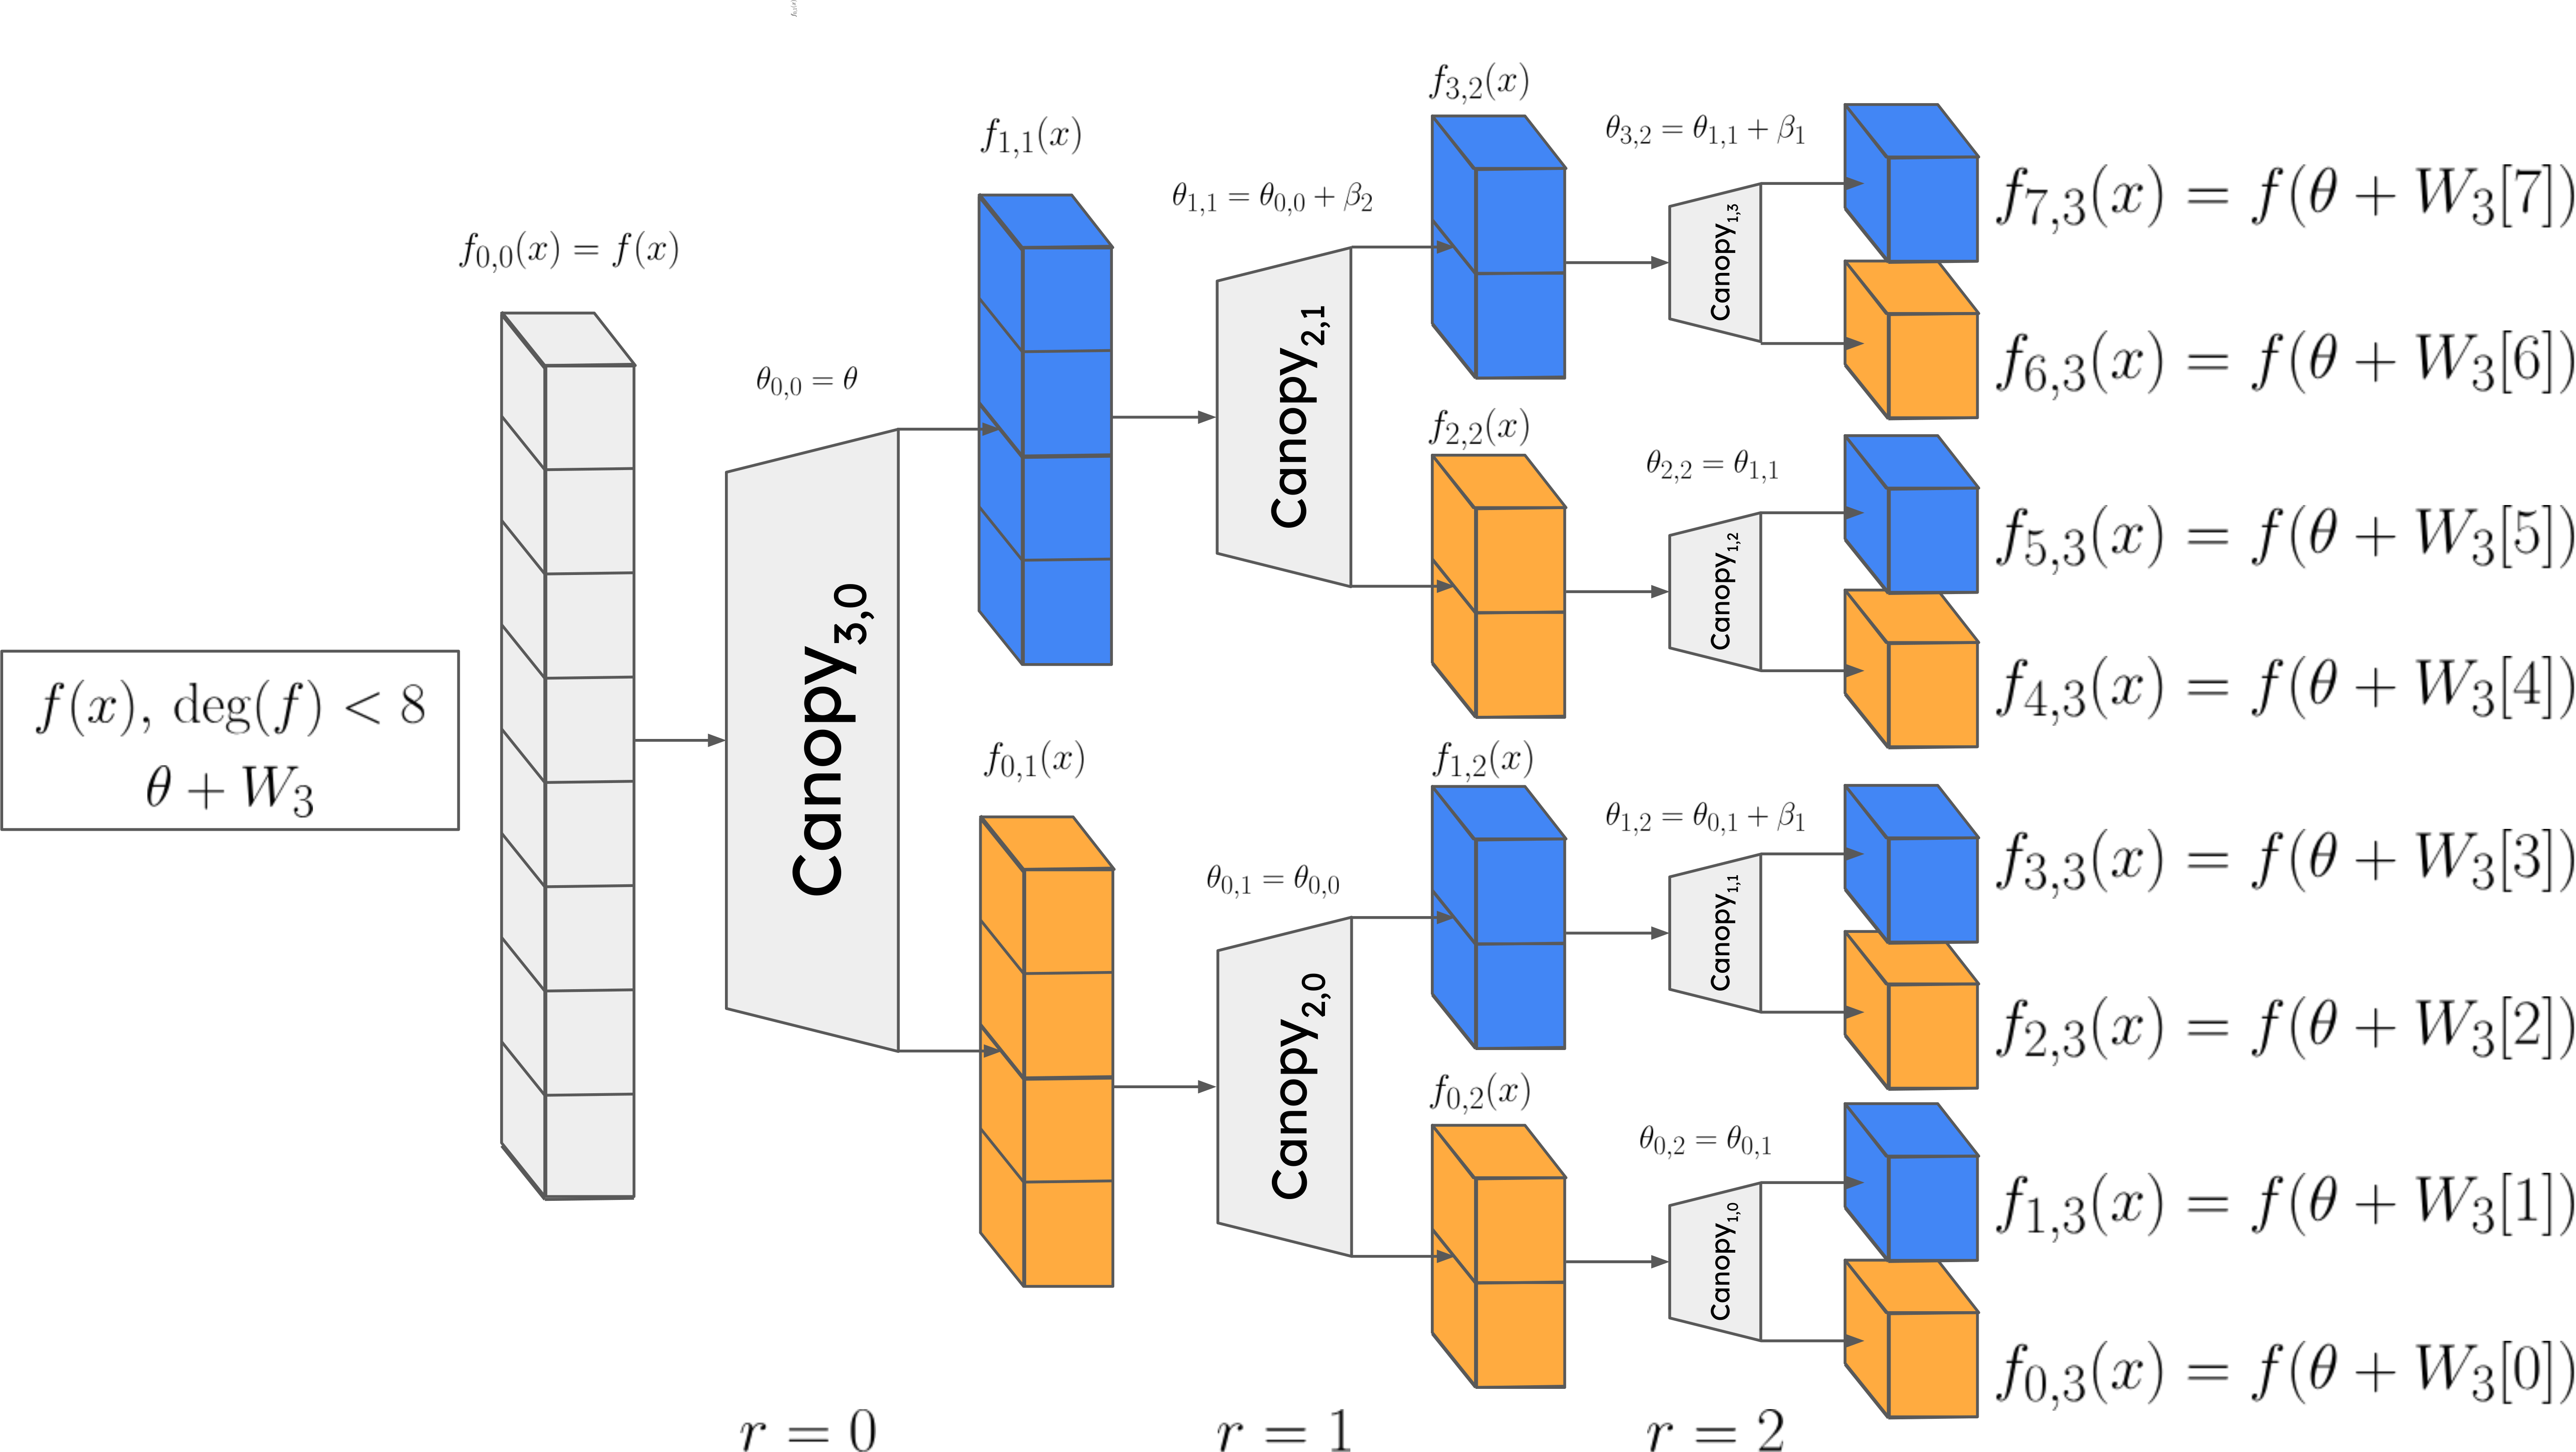
\includegraphics[width=0.8\linewidth]{Figures/Canopy.jpg}
	%     \caption{\small Cantor FFT algorithm of length $n = 2^3$ which evaluates $f(x)\in\mathbb{F}[x]$ of degree $<8$ over $\theta$ + $W_3$, where $\theta \in \mathbb{F}_{2^k}$ and $W_3$ is the Cantor special basis.}
	%     \label{fig:Canopy}
	% \end{figure}%\vspace{-100pt}

The $\mathsf{Canopy}_{p, i}$ determines $\theta_{i, r}$ and then evaluate $\mathbb{Z}_{W_{p-1}}(\theta_{i, r})$, which is necessary for running Algorithm~\ref{Algo:Polynomial Division}.  Let Cantor algorithm evaluate  $f(x)$ of degree $< 2^m$ over $\theta + \langle \beta_0 = 1, \beta_1, \ldots, \beta_{m-1} \rangle$.  
% Here, we describe how to efficiently determine $\theta_{i, r}$ for each $\mathsf{Canopy}_{p, i}$. 
Let $\theta_{0, 0} = \theta$, and for $1 \leq r \leq m-1$ and $0 \leq i \leq 2^r - 1$, $\theta_{i, r}$ is determined recursively according to the following rules:

\begin{equation*}
	\theta_{i, r} =
	\begin{cases}
		\theta_{i / 2, r - 1} & \text{if } i \bmod 2 = 0,\\
		\theta_{(i - 1) / 2, r - 1} + \beta_{p} & \text{if } i \bmod 2 = 1,
	\end{cases}
\end{equation*}
% \begin{align*}
	%     \theta_{2i, r+1} &= \theta_{i, r}, \\
	%     \theta_{2i + 1, r+1} &= \theta_{i, r} + \beta_{m-r}.
	% \end{align*}
where $p=m-r$. This equation can be simplified to 
$
\theta_{i, r} = \theta_{\lfloor i / 2 \rfloor, r - 1} + (i \bmod{2}) \beta_{p},
$
and can be written as,
\begin{equation*}
	\theta_{i, r} = \theta + \sum_{j=0}^{r - 1} \left( \lfloor \frac{i}{2^j} \rfloor \bmod{2} \right) \beta_{p+j} = \theta + \sum_{j=0}^{r - 1} i_j \, \beta_{p+j},
\end{equation*}
where $i = i_0 + i_12 + i_22^2 + \ldots + i_{r-1}2^{r-1}$ ($i_j \in \mathbb{F}_2$), denotes the binary representation of $i$. Then, to evaluate $\mathbb{Z}_{W_{p-1}}(\theta_{i, r})$, we employ the rule $S^{i}(\beta_{i+\ell}) = \beta_{\ell}$ provided earlier in this section to simplify the computation. Specifically, we write $\mathbb{Z}_{W_{p-1}}(\beta_{p-1 + j}) = \beta_j$. Therefore $\mathbb{Z}_{W_{p-1}}(\theta_{i, r})$ can be evaluated as
\begin{equation*}
	\setlength{\jot}{3pt}  % Reduces space between lines in multi-line equations
	\mathbb{Z}_{W_{p-1}}(\theta_{i, r}) =  \mathbb{Z}_{W_{p-1}}(\theta) + \sum_{j=0}^{r - 1} i_j \, \beta_{j+1},
\end{equation*}
where \(\mathbb{Z}_{W_{p-1}}(\theta)\) is evaluated at each round while constructing \(\zbu_{p-1}\) from \(\mathbb{Z}_{W_{p-1}}(x)\) during Algorithm~\ref{Algo:Vanishing Polynomial}. The computation of \(\mathbb{Z}_{W_{p-1}}(\theta)\) is shared across all the \(\mathsf{Canopy}\) modules in each row since the vanishing polynomial remains consistent. 

\begin{algorithm}[h]
	\caption{$\mathsf{Canopy}_{p, i}$ ($\fbu_\text{in}$, $\{\beta_0, \beta_1, \ldots, \beta_{m-1}\}$, $\zbu_{p-1}$, $\mathbb{Z}_{W_{p-1}}(\theta)$, $p$, $i$)}
	\label{Algo:Canopy}
	\begin{algorithmic}[1]
		\Require $\fbu_\text{in}$, $\{\beta_0, \beta_1, \ldots, \beta_{m-1}\}$ is the Cantor special basis, 
		$\zbu_{p-1} = (\zeta_0, \zeta_1, \ldots, \zeta_{2^{\text{wt}(i)}-2})$, 
		$\mathbb{Z}_{W_{p-1}}(\theta) \in \mathbb{F}_{2^k}$, 
		$p = m-r$, and $i = (i_0, i_1, i_2, \ldots, i_r)$.
		\Ensure $\fbu_\text{out}$
		
		\State $\psi_{i, r} \gets \mathbb{Z}_{W_{p-1}}(\theta)$
		
		\For{$j = 0$ to $r-1$}
		\State $\psi_{i, r} \gets \psi_{i, r} + i_j \times \beta_{j+1}$ \label{line:canopy-psi}
		\EndFor
		
		\State $\fbu_\text{out} \gets$ \Call{Polynomial Division}{$\fbu_\text{in}$, $\zbu_{p-1}$, $\psi_{i, r}$, $p$, $i$} \Comment{Algorithm \ref{Algo:Polynomial Division}, where $\mathbb{Z}_{W_{p-1}}(\theta_{i,r}) = \psi_{i, r}$}  
		
		\State \Return $\fbu_\text{out}$
	\end{algorithmic}
\end{algorithm}


\begin{algorithm}[h]
	\caption{Cantor Algorithm ($\fbu_\text{in}$, $\theta$, $\{\beta_0, \beta_1, \ldots, \beta_{m-1}\}$)}
	\label{Algo:Cantor_Implementation}
	\begin{algorithmic}[1]
		\Require $\fbu_\text{in}$ is a vector of size $2^m$ representing the coefficients in $f(x)$ (where $\deg{f} < 2^m$), 
		$\theta \in \mathbb{F}_{2^k}$ is the affine shift, 
		and $\{\beta_0, \beta_1, \ldots, \beta_{m-1}\}$ is the Cantor special basis.
		\Ensure $\fbu_\text{out}$ is the vector of evaluations of $f(x)$ over $\theta + \langle \beta_0, \beta_1, \ldots, \beta_{m-1} \rangle$.
		
		\For{$r = 0$ to $m-1$}
		\State $p \gets m - r$
		\State $\zbu_{p-1}, \mathsf{eval} \gets$ \Call{Vanishing Polynomial}{$p-1$, $\theta$} \Comment{Algorithm \ref{Algo:Vanishing Polynomial}} \label{line:cantor-vanishing}
		
		\For{$i = 0$ to $2^r - 1$}
		\State \Call{$\mathsf{Canopy}_{p, i}$}{$\fbu_\text{in}$, $\{\beta_0, \beta_1, \ldots, \beta_{m-1}\}$, $\zbu_{p-1}$, $\mathsf{eval}$, $p$, $i$} \Comment{Algorithm \ref{Algo:Canopy}}
		\EndFor
		\EndFor
		
		\State \Return $\fbu_\text{out}$
	\end{algorithmic}
\end{algorithm}


Algorithm~\ref{Algo:Canopy} details the steps within the \(\mathsf{Canopy}_{p, i}\) module, and Algorithm~\ref{Algo:Cantor_Implementation} describes the implementation of the Cantor algorithm based on those modules. 

\subsection{Detailed Cost Analysis}
At the $r$th iteration of the algorithm, we perform $2^{r}$ divisions by the polynomial $\mathbb{Z}_{W_{m-r-1}}(x)$. Consequently, the total number of additions resulting from polynomial division in the Cantor additive FFT is given by

\begin{equation*}
	\begin{aligned}
		\displaystyle{\sum_{r=0}^{m-1} 2^r \cdot 2^{m-r-1} \big( 2^{\text{wt}(m-r-1)}-1 \big) }
		= 2^{m-1} \displaystyle{\sum_{r=0}^{m-1} 2^{\text{wt}(r)} } - m2^{m-1}
	\end{aligned}
\end{equation*}

From Steps~\ref{Step:CantorLeftSib} and \ref{Step:CantorRightSib} of Algorithm~\ref{Algo:Polynomial Division}, we know that for the input polynomial in the $(r+1)$th iteration, we require $2 \times 2^r$ polynomial additions, each of degree less than $2^{m-r-1}$. This leads to a total of  $\sum_{r=0}^{m-1} 2\cdot 2^{r} \cdot 2^{m-r-1}=2^m m$ additions. Therefore, the total number of additions in the Cantor additive FFT is given by \[2^m m + 2^{m-1} \displaystyle{\sum_{r=0}^{m-1} 2^{\text{wt}(r)} } - m2^{m-1}= \frac{1}{2} n\log_2 n + \frac{1}{2}n \sum_{r=0}^{\log_2(n)-1} 2^{\text{wt}(r)}.\]

% \begin{equation*}
	%     \begin{aligned}
		%         &\displaystyle{\sum_{r=0}^{m-1} 2\cdot 2^{r} \cdot 2^{m-r-1} } + 2^{m-1} \displaystyle{\sum_{r=0}^{m-1} 2^{\text{wt}(r)} } - m2^{m-1}\\
		%         &= \frac{1}{2} 2^m m + \frac{1}{2} 2^m \displaystyle{\sum_{r=0}^{m-1} 2^{\text{wt}(r)} }= \frac{1}{2} n\log_2 n + \frac{1}{2}n \sum_{r=0}^{\log_2(n)-1} 2^{\text{wt}(r)}.
		%     \end{aligned}
	% \end{equation*}

This provides an exact count of the additions required in the Cantor additive FFT, whereas previous works, to the best of our knowledge, have only established upper bounds.

On the other hand, from Step~\ref{Step:CantorLeftSib} of Algorithm~\ref{Algo:Polynomial Division}, we know that for the input polynomial in the $(r+1)$th iteration, we require $2^r \times 2^{m-r-1}= 2^{m-1}$ multiplications. Thus, the number of multiplications in the Cantor additive FFT is given by
\(\sum_{r=0}^{m-1} 2^{m-1} = \frac{1}{2} n \log_2 n .\)

If the Cantor additive FFT is performed over a subspace $W_m$, due to Step~\ref{Step:CantorLeftSib} of the Algorithm~\ref{Algo:Polynomial Division}, we must account for a reduction of $\sum_{r=0}^{m-1} 2^{m-r-1}=2^m-1=n-1$ in both additions and multiplications. Thus, the costs for additions and multiplications are changed to
$\frac{1}{2} n\log_2 n + \frac{1}{2}n \sum_{r=0}^{\log_2(n)-1} 2^{\text{wt}(r)} -n +1$ and $\frac{1}{2} n \log_2 n-n+1$, respectively.
% In our instantiations of the Cantor algorithm, we can precompute some values that are independent of the input polynomial and only depend on the length of the FFT algorithm (i.e., the upper bound degree for the polynomial). Therefore, these values can be precomputed once for the Cantor algorithm of length $n$ and then used for evaluations of any polynomial whose degree is $< n = 2^m$. In the next section we suggest an algorithm for the precomputation.

\subsection{Precomputation} \label{sec:cantor_precmp}
% To avoid wasting computational power by recomputing certain values when the FFT algorithm is used to evaluate polynomials of the same degree over and over again, over the same evaluation set (i.e., $\theta + W_m$), we present our precomputation algorithm, which is executed once and stores the reused values in memory.

% In our instantiations of the Cantor algorithm, we can precompute some values that are independent of the input polynomial and only depend on the length of the FFT algorithm (i.e., the upper bound degree for the polynomial). Therefore, these values can be precomputed once for the Cantor algorithm of length $n$ and then used for evaluations of any polynomial whose degree is $< n = 2^m$. In this section, we suggest an algorithm for the precomputation.

The computations of $\mathbb{Z}_{W_{p-1}}(\theta_{i, r})$ for each \(\mathsf{Canopy}_{p, i}\), denoted as $\psi_{i, r}$ in Line \ref{line:canopy-psi} of Algorithm \ref{Algo:Canopy}, and the computation of the vanishing polynomials in Line \ref{line:cantor-vanishing} of Algorithm \ref{Algo:Cantor_Implementation}, do not depend on the input polynomial. 
The storage required to store the precomputed values for the Cantor algorithm of length $n = 2^m$ is 
$
\sum_{i=0}^{m-1} \left(2^{\text{wt}(i)} - 1\right)
$
integers to store $\mathbf{Z} = (\zbu_0, \zbu_1, \ldots, \zbu_{m-1})$ and $2^m - 1$ field elements to store $\boldsymbol{\Psi} = (\boldsymbol{\psi}_0, \boldsymbol{\psi}_1, \ldots, \boldsymbol{\psi}_{m-1})$, where $\boldsymbol{\psi}_r = ( \psi_{0,r}, \psi_{1,r}, \ldots, \psi_{2^r-1,r} )$. Algorithm \ref{Algo:Cantor_Precomp} in Appendix \ref{sec:ap-additional_algorithms} describes the precomputation algorithm. 

For a special case where the affine shift $\theta$ is an element of the Cantor special basis, we do not have to pre-compute all $\mathbb{Z}_{W_{p-1}}(\theta_{i, r})$, since these values are only combinations of the cantor basis. In this case we can precompute the lookup table where each store the combinations of subset of Cantor basis elements. 

\section{Gao-Mateer Algorithm Building Blocks}\label{Sec:Gao-implementation}

% Similar to the Cantor algorithm implementation, an iterative implementation of the Gao-Mateer algorithm is more efficient than a recursive approach, particularly in terms of memory usage and stack management. Thus, 
The Gao-Mateer FFT implementation of length $n = 2^m$ consists of $2m$ iterative rounds to evaluate a polynomial $f(x) \in \mathbb{F}_{2^k}[x]$ of degree $< 2^m$ over the affine subspace $\theta + W_m$, where $\theta \in \mathbb{F}_{2^k}$ and $W_m = \langle \beta_0, \beta_1, \ldots, \beta_{m-1} \rangle$. % such that $\beta_1, \ldots, \beta_{m-1} \in \mathbb{F}_{2^k}$ are linearly independent over $\mathbb{F}_2$.

We describe the Gao-Mateer algorithm through two primary modules: the \textsf{Expand} module and the \textsf{Aggregate} module.  \textsf{Expand} is an $r$-round algorithm where in each round $0 \leq r \leq m - 1$, it expands $2^r$ polynomials of degree $< 2^{m-r}$ into $2^{r+1}$ smaller polynomials of degree $<2^{m-r-1}$. Similar to our Cantor algorithm implementation, only one vector of length $2^m$ denoted as $\fbu$ is required to store all the polynomials in each round. \textsf{Aggregate} is an $r$-round algorithm that takes the output of \textsf{Expand}, and iteratively folds them over $r$ rounds, ultimately producing the evaluations of $f(x)$ on $\theta + W_m$. In the following, we start by presenting the Taylor expansion algorithm, which serves as the core component of \textsf{Expand}.

% Line \ref{line:gao-last_step_evaluation} of Algorithm \ref{Algo:Gao} which evaluates polynomials of degree $<2$ at $\theta_0 + \langle \beta_{m-1,0}\rangle$ is the step that \textsf{Expand} modules algorithm terminates and \textsf{Aggregate} modules starts. Such that, in the last round of the \textsf{Expand} modules, the coefficients of the degree-one terms in those polynomials are multiplied by the scaling factor denoted as $\beta_{m-1,0}$. Then in the first round of 

% The evaluating polynomials of degree $<2$, as described in Line \ref{line:gao-last_step_evaluation} of Algorithm \ref{Algo:Gao}, the coefficients of the degree-one terms in these polynomials are multiplied by the scaling factor during the final round of the \textsf{Expand} module. The remaining steps are completed in the first round of the \textsf{Aggregate} module.



\subsection{Taylor Expansion} \label{sec:Taylor Expansion}

The Taylor expansion algorithm implemented in~\cite{libiop} is described in Algorithm \ref{Algo:TaylorExpansion}, where the input parameter $r$ specifies how many iterations are skipped. 
% Specifically, the algorithm runs for $m - r - 1$ iterations for the input length of $2^m$. Algorithm \ref{Algo:TaylorExpansion}, on input of size $n = 2^m$ and parameter $r$, involves $2^{m-1}(m - r - 1)$ finite field additions. In the next section, we present our \textsf{Expand} module where we employed an alternative approach, as implemented in \cite{libiop}.



\begin{algorithm}[h]
	\caption{Taylor Expansion ($\fbu_\text{in}, r$)}
	\label{Algo:TaylorExpansion}
	\begin{algorithmic}[1]
		\Require $\fbu_\text{in} = (c_0,c_1,\ldots,c_{n-1})$ and $r$ denotes the number of rounds reduction.
		\Ensure $\fbu_\text{out}$
		
		\State $k \gets m - 2$
		
		\While{$k \ge r$}
		\State $j \gets 0$
		
		\While{$j \leq n - 4\cdot2^k$}
		\Comment{The following for-loop implements $\mathsf{T}_{4\cdot2^k}$}
		\For{$i = 0$ to $2^k - 1$}
		\State $c_{2\cdot2^k + i + j} \gets c_{2\cdot2^k + i + j} + c_{3\cdot2^k + i + j}$
		\State $c_{2^k + i + j} \gets c_{2^k + i + j} + c_{2\cdot2^k + i + j}$
		\EndFor
		\State $j \gets j + 4\cdot2^k$ \Comment{Sets the offset for the starting indices of $\mathsf{T}_{4\cdot2^k}$ modules}
		\EndWhile
		
		\State $k \gets k - 1$
		\EndWhile
		
		\State \Return $\fbu_\text{out} \gets (c_0,c_1,\ldots,c_{n-1})$
	\end{algorithmic}
\end{algorithm}


\subsection{Expand Module}

The \textsf{Expand} module involves multiple invocations of Algorithm \ref{Algo:TaylorExpansion}, polynomial scaling (e.g., $f(\beta_m x)$), and computing basis vectors and shifts for the \textsf{Aggregate} module. 
As discussed in Section \ref{sec:Taylor Expansion}, we omit even-odd rearrangements, 
% which alter the order of the coefficients in the polynomials embedded in $\fbu$, 
so the coefficients of terms with the same degree are placed next to each other. This allows \textsf{Expand} to multiply consecutive elements by the same scaling factor. 

In the last round of the \textsf{Expand} module, $\fbu$ is rearranged in bit-reversal order. Let the bit-reversed index of $j$ be denoted as $j\text{-}\mathsf{rev}$. During the bit-reversal rearrangement process, the elements \( c_j \) where \( j = j\text{-}\mathsf{rev} \) are not swapped. These elements are referred to as fixed elements. For an input of length \( n = 2^m \), the number of fixed elements is \( 2^{\lceil m/2 \rceil} \). Consequently, the algorithm requires \( 6 \times \frac{2^m - 2^{\lceil m/2 \rceil}}{2} \) memory accesses, as each swap involves 3 memory reads and 3 memory writes. Algorithm \ref{Algo:Expand} details the \textsf{Expand} module. The Bit-Reversal Rearrangement algorithm is described in Algorithm \ref{Algo:Bit Reversal} in Appendix \ref{sec:ap-additional_algorithms}.

% Next, we introduce the \textsf{Aggregate} module, the second building block of the Gao-Mateer algorithm.




%%%%%%%%%%%%%%%%%%%%%%%%%%%%%%%%%%%%%%%%%%%%%
\begin{algorithm}
	\caption{\textsf{Expand} ($\fbu_\text{in}, \theta, \{\beta_{0,0}, \ldots, \beta_{0, m-1}\}$)}
	\label{Algo:Expand}
	\begin{algorithmic}[1]
		\Require $\fbu_\text{in} = (c_0,c_1,\ldots,c_{n-1})$, which represents $f(x) \in \mathbb{F}[x]$ of degree $< n = 2^m$, 
		$\theta \in \mathbb{F}_{2^k}$ is the affine shift, 
		and $\beta_{0,i} \in \mathbb{F}_{2^k}$ are the basis of $W_m$.
		\Ensure $\fbu_\text{out}$, $\boldsymbol{\theta} = (\theta_0, \ldots, \theta_{m-1})$, 
		$\boldsymbol{\Gamma} = (\mathbf{G}_0 = \emptyset, \mathbf{G}_1, \ldots, \mathbf{G}_{m-1})$, 
		where $\theta_r$ and $\mathbf{G}_r = \{\gamma_{r,0},\ldots, \gamma_{r,r-1}\}$ denote the affine shift and basis corresponding to round $r$ of the \textsf{Aggregate} module.
		
		\For{$r = 0$ to $m-1$}
		\Comment{Scaling polynomials:}
		\State $\psi \gets 1$ \Comment{$\psi$ denotes the scaling factor of each term} \label{line:expand-psi-init}
		\State $\mathsf{offset} \gets 2^r$
		
		\While{$\mathsf{offset} \leq 2^m -1$}
		\For{$i = 0$ to $2^r - 1$}
		\State $c_{\mathsf{offset}+i} \gets c_{\mathsf{offset}+i} \times \psi$ \label{line:expand-scale}
		\EndFor
		\State $\psi \gets \psi \times \beta_{r,m-r-1}$ \label{line:expand-psi}
		\State $\mathsf{offset} \gets \mathsf{offset} + 2^r$
		\EndWhile
		
		\State $(c_0,\ldots,c_{n-1}) \gets$ \Call{Taylor Expansion}{$(c_0,\ldots,c_{n-1}), r$} \Comment{Algorithm \ref{Algo:TaylorExpansion}} \label{line:expand-taylor}
		
		\For{$i = 0$ to $m-r-2$}
		\State $\gamma_{m-r-1,i} \gets \beta_{r,i} \times \beta_{r,m-r-1}^{-1}$ \label{line:expand-gamma_computaion}   
		\State $\beta_{r+1,i} \gets \gamma_{m-r-1,i}^2 + \gamma_{m-r-1,i}$ \label{line:expand-beta_computaion}
		\EndFor
		\State $\mathbf{G_{m-r-1}} \gets (\gamma_{m-r-1,0}, \ldots, \gamma_{m-r-1,m-r-2})$
		\State $\theta_{m-r-1} \gets \theta \times \beta_{r,m-r-1}^{-1}$ \label{line:expand-theta1_computaion}
		\State $\theta \gets \theta_{m-r-1}^2 + \theta_{m-r-1}$ \label{line:expand-theta2_computaion}
		\EndFor
		
		\State $(c_0,\ldots,c_{n-1}) \gets$ \Call{Bit Reverse Rearrangement}{$(c_0,\ldots,c_{n-1})$}
		
		\State \Return $\fbu_\text{out} \gets (c_0,c_1,\ldots,c_{n-1})$
	\end{algorithmic}
\end{algorithm}






% Let \( f(x) \) be a polynomial of degree \( <n=2^m \), and let \( W_m = \langle \beta_0, \beta_1, \cdots, \beta_{m-1} \rangle \).



% In the original Gao FFT algorithm, as suggested in Algorithm \ref{Algo:Gao}, the $\textsf{TE}(\fbu, n)$ algorithm is applied to \( f(\beta_{m-1} x) \) and outputs $f_0(x)$ and $f_1(x)$ after the even-odd arrangements of $\fbu$ indices as described in the last step of Algorithm \ref{Algo:TaylorExpansion}. 

% Subsequently, again Algorithm \ref{Algo:TaylorExpansion} is separately applied to the first and second half of $\fbu$, representing two polynomials \( f_0(\beta_{1,m-2} x) \) and \( f_1(\beta_{1,m-2} x) \), each of degree \( <n=2^{m-1} \), where \( \beta_{1,m-2} = (\gamma_{m-1})^2 + \gamma_{m-1} \) and \( \gamma_{m-1} = \beta_{m-2}\beta_{m-1}^{-1} \). 

% Alternatively, instead of 

% Subsequently, the \textsf{TE} algorithm is applied to polynomials of smaller degree, consistent with the original Gao FFT algorithm.

% The subsequent rounds of the \textsf{Expand}  module, which is explained in the next section, of half size is applied to the outputted polynomials.






% employs the Taylor expansion algorithm to divide $2^r$ polynomials of degree $< 2^{m-r}$ into $2^{r+1}$ smaller polynomials of degree $<2^{m-r-1}$. 


\subsection{Aggregate Module}

The \textsf{Aggregate} module combines $2^r$ adjacent elements in $\fbu$ during round $r$, where $0 \leq r \leq m-1$. Let $\{\eta_0, \eta_1, \ldots, \eta_{2^{r}-1} \}$ denote the elements in the affine subspace $\theta_r + \langle \gamma_{r,0}, \ldots, \gamma_{r,r-1} \rangle$ provided in the \textsf{Expand} module. At each round $r$, it computes those elements by spanning the mentioned affine subspace, which requires a total of $\sum_{i=0}^{r-1} 2^i = 2^r -1$ finite field additions and $2^r + r$ memory accesses: $r$ memory reads for retrieving the $\gamma_i$s and $2^r$ memory writes for storing the $\eta_k$s. The algorithm for computing $\eta_k$s is described in Algorithm \ref{Algo:Span} in Appendix \ref{sec:ap-additional_algorithms}.

% Algorithm \ref{Algo:Aggregate} describes the textsf{Aggregate} module te\tex. 



\begin{algorithm}
	\caption{\textsf{Aggregate} ($\fbu_\text{in}, \boldsymbol{\Gamma}, \boldsymbol{\theta}$)}
	\label{Algo:Aggregate}
	\begin{algorithmic}[1]
		\Require $\fbu_\text{in} = (c_0,c_1,\ldots,c_{n-1})$ is a vector of length $ n = 2^m$, 
		$\boldsymbol{\theta} = (\theta_0, \ldots, \theta_{m-1})$, 
		$\boldsymbol{\Gamma} = (\mathbf{G}_0 = \emptyset, \mathbf{G}_1, \ldots, \mathbf{G}_{m-1})$, 
		where $\theta_r$ and $\mathbf{G}_r = \{\gamma_{r,0},\ldots, \gamma_{r,r-1}\}$ denote the affine shift and basis corresponding to round $r$.
		\Ensure $\fbu_\text{out}$ is the vector of evaluations of $f(x)$ over $\theta + W_m$.
		
		\For{$r = 0$ to $m-1$}
		\State $\{\eta_0, \eta_1, \ldots, \eta_{2^{r}-1} \} \gets \mathsf{Span}(\mathbf{G}_r, \theta_r)$
		\For{$j = 0$ to $2^{m-r-1}-1$}
		\State $d \gets j \cdot 2^{r+1}$
		\For{$i = 0$ to $2^r-1$}
		\State $c_{d+i} \gets c_{d+i} + c_{d+2^r+i} \times \eta_i$ \label{Step:AlgAgreeM1}
		\State $c_{d+2^r+i} \gets c_{d+2^r+i} + c_{d+i}$ \label{Step:AlgAgreeM2}
		\EndFor
		\EndFor
		\EndFor
		
		\State \Return $\fbu_\text{out} \gets (c_0,c_1,\ldots,c_{n-1})$
	\end{algorithmic}
\end{algorithm}



\subsection{Detailed Cost Analysis}\label{Sec:Cost-GM}
We now compute the number of multiplications and additions required by the algorithm. From Algorithm~\ref{Algo:Expand}, we know that at the $r$th iteration, we need to scale $2^r$ polynomials, each of degree $2^{m-r}$. Thus, the multiplication for the scaling is given by
$\sum_{r=0}^{m-1} 2^r \cdot (2^{m-r}-1)= 2^m m - \sum_{r=0}^{m-1} 2^r= n \log_2 n -n +1$.

From Algorithm~\ref{Algo:Aggregate}, we know that at the $r$th iteration, the number of required multiplications is $2^r \cdot 2^{m-r-1}=2^{m-1}$. Thus, the total multiplication cost in Algorithm~\ref{Algo:Aggregate} is $\sum_{r=0}^{m-1} 2^{m-1}=\frac{1}{2} n \log_2 n.$ Therefore, the total number of multiplications in the Gao-Mateer algorithm is given by $n \log_2 n -n +1 + \frac{1}{2} n \log_2 n = \frac{3}{2} n \log_2 n -n +1$.
% \[n \log_2 n -n +1 + \frac{1}{2} n \log_2 n = \frac{3}{2} n \log_2 n -n +1 .\]

From Algorithm~\ref{Algo:TaylorExpansion}, we know that in the $r$th iteration, the number of additions due to the Taylor expansion is $2^{m-1}(m-r-1)$. Thus, the total number of additions required for the Taylor expansions is $\sum_{r=0}^{m-2}2^{m-1}(m-r-1) = 2^{m-2}m(m-1)$. Also, in Algorithm~\ref{Algo:Aggregate}, we know that at the $r$th iteration, the number of required additions is $2 \cdot 2^r \cdot 2^{m-r-1} =2^{m}$. Therefore, the total addition cost for the algorithm is given by
\(2^{m-2}m(m-1) + m\cdot 2^m= \frac{1}{4}n(\log_2n)^2 + \frac{3}{4}n\log_2n. \)

When performing the FFT over a subspace, at each $r$th iteration of Algorithm~\ref{Algo:Aggregate}, we have $\eta_0=0$. Thus, for Steps~\ref{Step:AlgAgreeM1} and \ref{Step:AlgAgreeM2}, we need no multiplications are required, and only one addition is needed. Consequently, we must account for a reduction of $\sum_{r=0}^{m-1} 2^{m-r-1}=2^m-1=n-1$ in both additions and multiplications. Therefore, the costs for multiplications and additions are changed to
$\frac{3}{2} n \log_2 n -2n +2$ and  $\frac{1}{4}n(\log_2n)^2 + \frac{3}{4}n\log_2n-n+1$, respectively.

\subsection{Optimization for Cantor Special Basis}\label{Sec:Gao-optimization-Cantor_basis}
% We know that evaluating $f(x)$ over $\theta + W_m$ is equivalent to evaluating $g(x)$ over $(\theta_0 + G) \cup (1 + \theta_0 + G)$, where $\theta_0 = \beta_{m-1}^{-1} \theta$. Thus, to compute $g(x)=f(\beta_{m-1}x)$, we need to scale the function $f(x)$, which requires $n-1$ multiplications. However, by simply choosing $\beta_{m-1} = 1$, we can eliminate these $n-1$ multiplications. However, for the next iteration, we need to scale the functions $f_0(x)$ and $f_1(x)$ by $\beta_{m-1}^2 + \beta_{m-1}$, as we need to evaluate $f_0(x)$ and $f_1(x)$ over $\theta_0^2 + \theta_0 + D$. 
% where
% \[
%     D = \langle \alpha^{2(m-1)} + \alpha^{m-1}, \ldots, \alpha^2 + \alpha \rangle.
% \]
% Thus, we need $2 \times (2^{m-1} - 1) = 2^m - 2$ multiplications for the scaling. This scaling is required in each iteration until $D$ is reduced to dimension 1. The interesting question is whether we can avoid scaling in every iteration.

If we have a Cantor special basis of dimension $m$, we can avoid the scaling in every iteration. We know that a Cantor special basis satisfy the following

\begin{equation*}
	\begin{aligned}
		&\beta_{0}=1 \quad \text{and } S(\beta_{i})=\beta_{i}^2+\beta_{i}=\beta_{i-1} \quad \text{for } 1\leq i \leq m-1,
	\end{aligned}
\end{equation*}
where $S(x)=x^2+x$. In addition, we know that $S^{i}(\beta_{i})=\beta_{0}=1$ for $0 \leq i \leq m-1$ and $S^{i+\ell}(\beta_{i+\ell})=\beta_{\ell}$ for any $i,\ell \geq 0$ with $i+\ell\leq m-1$. Now, consider the Cantor special basis in the reversed order, i.e.,
\begin{equation*}
	\begin{aligned}
		W_m
		&= \langle \beta_{m-1},\beta_{m-2},\ldots,\beta_{1},1  \rangle= \langle \beta_{m-1},S(\beta_{m-1}),\ldots,S^{m-2}(\beta_{m-1}),1  \rangle.
	\end{aligned}
\end{equation*}

Thus, we have $G= \langle \beta_{m-1},S(\beta_{m-1}),\ldots,S^{m-2}(\beta_{m-1}))$ and 
\begin{equation*}
	\begin{aligned}
		D
		&= \langle S(\beta_{m-1}),S^2(\beta_{m-1}),\ldots,S^{m-1}(\beta_{m-1}))
		= \langle S(\beta_{m-1}),S^2(\beta_{m-1}),\ldots,1 \rangle.
	\end{aligned}
\end{equation*}

Thus, we do not need the scaling for the functions $f_0(x)$ and $f_1(x)$. Also, at the $j$-th iteration, $G$ and $D$ will be of the form 
\begin{equation*}
	\begin{aligned}
		G^{(j)}
		&= \langle S^{j}(\beta_{m-1}),S^{j+1}(\beta_{m-1}),\ldots,S^{m-2}(\beta_{m-1}) \rangle \quad \text{ and } \\
		D^{(j)}
		&= \langle S^{j+1}(\beta_{m-1}),S^{j+2}(\beta_{m-1}),\ldots,S^{m-1}(\beta_{m-1})=1 \rangle.
	\end{aligned}
\end{equation*}

Therefore, at each iteration there is no need for scaling. Also, due to the chosen basis, computing the basis elements in $G^{(j)}$ and $D^{(j)}$ does not require any multiplications or additions. This can be done simply by selecting one fewer element from $G^{(j-1)}$ and $D^{(j-1)}$.

\paragraph{Detailed cost analysis of the optimized algorithm} When using the Cantor basis in Algorithm~\ref{Algo:Expand}, no scaling is required for the polynomials. All other steps in Algorithms~\ref{Algo:Expand} and \ref{Algo:Aggregate} remain unchanged. Thus, the number of additions remains the same, as evaluated in Section~\ref{Sec:Cost-GM}. Consequently, the multiplication and addition costs are $\frac{1}{2}n\log_2n$ and $\frac{1}{4}n(\log_2 n)^2 + \frac{3}{4}n\log_2 n$, respectively.

% The number of additions remains unchanged, as evaluated in Section~\ref{Sec:Cost-GM}. Therefore, the total addition cost for the optimized algorithm is $\frac{1}{4}n(\log_2 n)^2 + \frac{3}{4}n\log_2 n$.

Furthermore, as discussed in Section~\ref{Sec:Cost-GM}, when performing the FFT over a subspace, the total multiplication and addition costs for the algorithm are $\frac{1}{2}n\log_2n - n+1$ and $\frac{1}{4}n(\log_2n)^2 + \frac{3}{4}n\log_2n - n +1$, respectively.

Thus, by using Cantor special basis in the Gao-Mateer algorithm, we can efficiently compute the additive FFT of $f(x)\in \F_{2^k}[x]$ over $\theta + W_m$ where $\F_{2^k}$ contain a subfield $\F_{2^{2^\ell}}$ with $m \leq 2^{\ell}$.

% Table~\ref{tab:FFTcomparisons} presents a comparison of the number of additions and multiplications required by the Cantor, Gao-Mateer, and LCH~\cite{LCH-FFT2016} FFTs with precomputation.

% \begin{remark}
	%     Note that the second algorithm in~\cite{Gao2010FFT} applies to the additive FFT of length $n = 2^m$, where $m = 2^t$, and utilizes the Cantor special basis. However, for a polynomial $f(x)$ of degree between $2^{2^{t-1}}$ and $2^{2^t}$, particularly when their degree is significantly less than $2^{2^t}$, a large number of zero-padding is required to extend the polynomial vector $\mathbf{f}$ to length $2^{2^t}$, resulting in unnecessary computational overhead. In contrast, our approach, which uses the Cantor special basis in their first algorithm, allows for handling polynomials of any degree for arbitrary values of $m$ without this restriction.
	% \end{remark}

% When we do the evaluation over a subspace, in the last iteration, the evaluation of $f(x)$ requires no multiplication and one additions which implies that the last iteration involves no multiplication and $2^{m-1}$ additions. Therefore, the total cost of multiplication and addition for the algorithm is $\frac{1}{2}n\log_2n-\frac{1}{2}n$ and $\frac{1}{4}n(\log_2n)^2 + \frac{3}{4}n\log_2n-\frac{1}{2}$, respectively.

\subsection{Precomputation}\label{sec:gao-precmp}

In this section, we introduce two levels of precomputation. The first level precomputes the set $\boldsymbol{\beta} = \{\beta_{0, m-1}, \ldots, \beta_{r, m-r-1}, \ldots, \beta_{m-1, 0} \}$, which is essential for determining the scaling factors. Additionally, it precomputes  $\boldsymbol{\Gamma} = (\mathbf{G}_0 = \emptyset, \mathbf{G}_1,  \ldots, \mathbf{G}_{m-1})$ and $\boldsymbol{\theta} = (\theta_0, \ldots, \theta_{m-1})$ required by the \textsf{Aggregate} module, initially provided by the \textsf{Expand} module. This precomputation requires $m$ finite field elements for $\boldsymbol{\beta}$ and $\boldsymbol{\theta}$, along with $\sum_{i=0}^{m-1} i = m(m-1)/2$ finite field elements for $\boldsymbol{\Gamma}$. Consequently, this algorithm stores a total of $(m^2+3m)/2$  finite field elements. 
For the  variant of the Gao-Mateer algorithm described in Section~\ref{Sec:Gao-optimization-Cantor_basis}, the scaling operation is omitted, and each basis $\mathbf{G}_r$ is defined as $\{\beta_0, \beta_1, \ldots, \beta_{r-1}\}$. Therefore, this level of precomputation is not applicable for that.

The second level of precomputation precomputes the powers of the actual scaling factors. Moreover, instead of storing the basis $\mathbf{G}_r$, it precomputes all elements in each affine subspace $\theta_r + \langle \gamma_{r,0}, \ldots, \gamma_{r,r-1} \rangle$. This requires storing $\sum_{r=0}^{m-1} (2^{m-r} - 1) = 2^{m+1} - m - 2$ finite field elements for all scaling factors stored in $\boldsymbol{\Psi} = (\boldsymbol{\psi}_0, \ldots, \boldsymbol{\psi}_{m-1})$ where $\boldsymbol{\psi}_r = (\psi_{r,1}, \ldots,   \psi_{r,2^{m-r}-1})$ and $\psi_{r,d} = \beta_{r, m-r-1}^d$. 
Also, it stores $\sum_{r=0}^{m-1} 2^r = 2^m - 1$ finite field elements for all computed elements stored in $\mathbf{H} = (\boldsymbol{\eta}_0, \ldots, \boldsymbol{\eta}_{m-1})$, where $\boldsymbol{\eta}_r = \{\eta_0, \ldots, \eta_{2^r-1}\}$ are elements in $\theta_r + \langle \gamma_{r,0}, \ldots, \gamma_{r,r-1} \rangle$. Consequently, this algorithm stores a total of $3 \cdot 2^m - m - 3$ finite field elements. For the optimized variant described in Section~\ref{Sec:Gao-optimization-Cantor_basis}, the scaling factor is not required, and we only need to obtain the elements in $\theta + \langle\beta_0, \beta_1, \ldots, \beta_{m-1}\rangle$, which equals $2^m$ finite field elements.

Algorithms~\ref{Algo:Gao_Precmp_lvl1} and \ref{Algo:Gao_Precmp_lvl2} in Appendix \ref{sec:ap-additional_algorithms} summarize those precomputations.


\section{Aurora FFT Complexity Analysis} \label{Sec:FFT_Calls_in_Aurora}
Given a target security parameter $\boldsymbol{\lambda}$, and subsets $H_1$ and $H_2$,
% where size of each is determined by the number of constraints and variables of a given R1CS relation respectively,
the size of the codeword domain (i.e., $|L|$) is determined. This size is important for the analysis of the FFT complexity of Aurora, as the input length of many FFT and IFFT instances is $|L|$. Before computing $|L|$, we need to review how the number of queries to the  codeword is determined based on the target security parameter.

\subsection{Soundness Errors: Queries and Repetition Analysis}
Given $\boldsymbol{\lambda}$, $\boldsymbol{\epsilon_q}$ and $\boldsymbol{\epsilon_i}$ represent query and interactive soundness errors such that
\(
\boldsymbol{\epsilon_q} + \boldsymbol{\epsilon_i} < 2^{-\boldsymbol{\lambda}},
\)
where $2^{-\boldsymbol{\lambda} - 1}$ is allocated to each. According to \cite[Theorem 4]{Aurora2019}, 
\[
\boldsymbol{\epsilon_i} = \left(\frac{\eta + 1}{|\mathbb{F}|}\right)^{\lambda_i} + \left(\frac{|L|}{|\mathbb{F}|}\right)^{\lambda'_i} + \epsilon^{\text{FRI}}_i,\text{ and } \boldsymbol{\epsilon_q} = \epsilon^{\text{FRI}}_q,
\]
where $ \left(\frac{\eta + 1}{|\mathbb{F}|}\right)^{\lambda_i}$ and $\left(\frac{|L|}{|\mathbb{F}|}\right)^{\lambda'_i}$ denote the lincheck and LDT soundness errors respectively. $\epsilon^{\text{FRI}}_i$ and   $\epsilon^{\text{FRI}}_q$ denote the interactive and query soundness errors in FRI, respectively. Each term in $\boldsymbol{\epsilon_i}$ gets $2^{-\boldsymbol{\lambda} - 3}$ and $\boldsymbol{\epsilon_q}$ gets $2^{-\boldsymbol{\lambda} - 1}$ soundness error bound. 
The codeword is queried during FRI. 
% where the number of queries is determined by $\epsilon^{\text{FRI}}_q$ and the localization parameter $\phi$. 
Given, the target proximity parameter in (\ref{eq:proximity_parameter}), the number of query repetitions in FRI is:
\begin{equation}\label{eq:num_queries}
	\lambda_q^\text{FRI} = \frac{\log(\epsilon^{\text{FRI}}_q)}{\log\left( 1 - \min\left(\delta,  \frac{1- 3\rho - 2^\phi/\sqrt{|L|}}{4} \right)  \right)}.  
\end{equation}
Moreover, the required lincheck and LDT repetition parameters are determined as:
\(
\lambda_i = \frac{-\boldsymbol{\lambda} - 3}{\log\left(\frac{\eta+1}{|\mathbb{F}|}\right)},\text{ and } \lambda'_i = \frac{-\boldsymbol{\lambda} - 3}{\log\left(\frac{|L|}{|\mathbb{F}|}\right)}.
\)



\subsection{Codeword Size}
The maximum degree of the polynomial in the codeword of size $|L|$ is $d = 2t+2\texttt{b}$ (according to Table \ref{tab:codewords}), where \texttt{b} is determined by the expected number of queries to the corresponding codeword.
% , to let \texttt{b} evaluations of the polynomial over $|L|$ be randomly distributed to achieve zero-knowledge. 
The number of queries to the codeword is $\texttt{b} = \lambda_q^\text{FRI} \cdot 2^{\phi}$, where according to (\ref{eq:num_queries}), $\lambda_q^\text{FRI}$ also relies on $|L|$. To solve this loop, we initialize $|L| = 4t/\rho$ and \texttt{b} as mentioned. Then, we check the following condition: Let $\texttt{r}=\lfloor\log(\rho|L|)/\phi\rfloor$ denote the number of reductions in FRI,  $d' = 2t + \texttt{b}-1$ (lincheck maximum degree) must be divisible by $2^{\texttt{r}\phi}$, otherwise, $d'$ must be increased to the nearest multiple of $2^{\texttt{r}\phi}$. Then, we check if the new $d' \leq \rho |L|$, otherwise, increase the dimension of $L$ by one. Again, we compute \texttt{b} and check if it is the same as it was; otherwise, we update that and again check the condition with the new $L$. This iteration is continued until the \texttt{b} remains unchanged, at which point $|L|$ is determined.

\subsection{Construction of $H_1$, $H_2$, and $L$}
Let $\{\beta_0, \beta_1, \dots, \beta_{k-1}\}$ represent basis elements of $\mathbb{F}_{2^k}$. Then, we construct subsets  $H_1=\langle \beta_0, \beta_1, \cdots \beta_{\lceil\log\eta\rceil} \rangle$ and $H_2 = \langle \beta_0, \beta_1, \cdots \beta_{
	\lceil\log(\mu + 1)\rceil} \rangle$ and the affine subspace $L= \beta_{
	\lceil\log(|L|)\rceil+1} + \langle \beta_0, \beta_1, \cdots \beta_{
	\lceil\log(|L|)\rceil} \rangle$. In this way,  $L \cap (H_1 \cup H_2) = \emptyset$. If the basis elements are Cantor special basis, the Cantor FFT can be used without precomputation due to this special construction, as detailed in Section \ref{sec:cantor_precmp}.

\subsection{FFT/IFFT Calls}
Table \ref{tab:fftcalls} summarizes the FFT and IFFT calls for computing the codewords in Table \ref{tab:codewords}. Virtual oracles are used for consistency checks, and are not included in the random combination of codewords input to the FRI protocol.

\vspace{-2em}
\begin{table}
	\centering
	\caption{ The FFT and IFFT calls in the Aurora zkSNARK protocol}
	{
		\label{tab:fftcalls}
		\begin{tabularx}{\linewidth}{>{\hsize=.38\hsize}XX}
			\toprule
			\textbf{FFT Calls} & \textbf{Description} \\
			\midrule
			$\lambda_i \times$ FFT of len. $|L|$ & Compute the masking oracle $\hat{\rbu}_\ell$: Evaluate the polynomial $r_\ell$ of degree $<2t+b-1$ over $L$, where $\ell \in [1,\lambda_i]$. \\
			\midrule
			
			(1) IFFT of len. $\kappa + 1$\newline
			(2) FFT of len. $\mu + 1$\newline
			(3) IFFT of len. $\mu + 1$\newline
			(4) FFT of len $|L|$
			& Compute the oracle $\hat{\fbu}_\wbu$: \newline
			(1) Interpolate $\vbu$ to get $f_{(1,\vbu)}$ of degree $<\kappa + 1$. \newline
			(2) Evaluate $f_{(1,\vbu)}$ over $H_2$. \newline 
			Then, computing $\fbu'_\wbu = {\wbu_{i-\kappa-1}[0:\mu-\kappa - 1] - \fbu_{(1,\vbu)}[\kappa+1:\mu]}$ \newline
			% $f_\wbu$ of degree $<\mu - \kappa$ \newline 
			(3) Interpolate $\fbu'_\wbu$ over $H_2$ to get $f'_\wbu$ of degree $< \mu + 1$. \newline
			Then, divide $f'_\wbu$ by $\mathbb{Z}_{\{h_0,\dots, h_{\kappa}\}}$ to get $f_\wbu$.\newline
			(4) Evaluate $f_\wbu^*$ over $L$.
			\\
			\midrule
			(1) $3 \times$ IFFT of len. $\eta$\newline
			(2) $3 \times$ FFT of len. $|L|$
			&
			Compute the oracles $\hat{\fbu}_{\mathbf{Az}}$, $\hat{\fbu}_{\mathbf{Bz}}$, and $\hat{\fbu}_{\mathbf{Cz}}$:\newline
			(1) Interpolate $\mathbf{Az}$, $\mathbf{Bz}$, and $\mathbf{Cz}$ to get $f_\mathbf{Az}$, $f_\mathbf{Bz}$, $f_\mathbf{Cz}$ of degree $<\eta$.\newline
			(2) Evaluate $f_\mathbf{Az}^*$, $f_\mathbf{Bz}^*$, $f_\mathbf{Cz}^*$ over $L$.
			\\
			\midrule
			$\lambda'_i \times$ FFT of len. $|L|$ & Compute the masking oracle $\hat{\rbu}'_\ell$: Evaluate the polynomial $r'_\ell$ of degree $<2t+2b$ over $L$, where $\ell \in [1,\lambda'_i]$. \\
			\midrule
			$\lambda_i \times$ IFFT of len. $t$ & Interpolate the polynomial $p_{\alpha_\ell}$ in (\ref{eq:pa}), where $\ell \in [1,\lambda_i]$. 
			\\
			\midrule
			$\lambda_i \times$ IFFT of len. $t$ & Interpolate the polynomial $p^{ABC}_{\alpha_\ell}$ in (\ref{eq:pa}), where $\ell \in [1,\lambda_i]$. 
			\\
			\midrule
			FFT of len. $|L|$ & Compute the virtual oracle $\hat{\fbu}_\zbu := \hat{\fbu}_\wbu \cdot \mathbb{Z}_{\{h_0,\dots, h_{\kappa}\}} + \hat{\fbu}_{(1,\vbu)}(h_i)$ which requires 
			Evaluating $f_{(1,\vbu)}$ over $L$.
			\\
			\midrule
			$\lambda_i \times 2 \times $FFT of len. $|L|$ & Compute virtual oracles $\hat{\mathbf{q}}_\ell^M := \hat{\fbu}_{\mathbf{Mz}}\cdot \hat{\mathbf{p}}_{\alpha_\ell} - \hat{\fbu}_\zbu \cdot \hat{\mathbf{p}}^{ABC}_{\alpha_\ell} $, where $\ell \in [1,\lambda_i]$ and $M \in \{A, B, C\}$, by evaluating $p_{\alpha_\ell}$ and $p^{ABC}_{\alpha_\ell}$ over $L$.
			\\
			\midrule
			(1) $\lambda_i \times $IFFT of len. $d$\newline where $d = 2^{\lceil\log(t+b)\rceil}$ \newline
			(2) $\lambda_i \times $FFT of len.
			$|L|$
			& Compute the oracle $\hat{\hbu}_\ell$:\newline
			(1) Interpolate $\sum_{M \in \{A, B, C\}} s^M_\ell \hat{\mathbf{q}}_\ell^M$ to get a  polynomial of degree less than the minimum power of two greater than $t + \texttt{b}$.%\newline
			Then, compute the polynomial $h$ according to Table \ref{tab:codewords}\newline
			(2) Evaluate $h$ over $L$
			\\
			\bottomrule
		\end{tabularx}
	}
\end{table}












% \begin{remark}
	%  \textcolor{blue}{    
		% "Note that in \cite{Gao2010FFT}, it discussed a case when $f(x)$'s degree is equal to $2^m$. But for our Cantor basis approach, we allow the degree of $f(x)$ be any". Please check whether this is correct! } 
	% \end{remark}

% \subsection{An efficient basis for the additive FFT}

% Let $t>s$,  the polynomial $f(x)$ have degree $<m=2^s$, and the additive FFT is to compute the evaluation of $f$ at $L$ iteratively.
% \[
% \begin{array}{ll}
	% B_0& =<\alpha^{t-1}, \cdots, \alpha, 1>\\
	% G_1& = <\alpha^{m-1}, \cdots, \alpha>\\
	% D_1& = <\delta(\alpha^{m-1}), \cdots, \delta(\alpha)>.
	% \end{array}
% \]
% This basis will save $m-1$ multiplications at the first step of the iteration. 
% At step $i$,the bases are
% \[
% \begin{array}{ll}
	% B_i& =D_i=<\beta_{m-1}, \cdots, \beta_i>\\
	% G_{i+1}& = <\beta_{m-1}\beta_i^{-1}, \cdots, \beta_{i+1}\beta_i^{-1}> =<\gamma_{m-1}, \cdots, \gamma_{i+1}>\\
	% D_{i+1}& = <\delta(\gamma_{m-1}), \cdots,   \delta(\gamma_{i+1})>.
	% \end{array}
% \]


% \textcolor{red}{Susanta: please put GM algorithm here, and take care of the ending layer, when the degree of $f$ satisfies that  $2^{s-v-1}\le deg(f) <2^{s-v}, v>0$, since it will be ended when $f(x)$ reduced to a linear polynomial, but $L$ only downs to a linear space with dimension $s-v$.  
	% This is the case we need, but GM's paper did not consider that. Please get the exactly complexity by counting the number of multiplications and additions. 
	% }










 %======================================================================
\chapter{Polaris zkSNARK Optimization}\label{ch:polaris}
%======================================================================

\section*{Declaration of Contributions}
This chapter is based on~\cite{Badakhshan2025Ursa} I have co-authored the paper and my main contributions are as follows:
\begin{itemize}
	\item Design of the GKR circuit for the Polaris \gls{zksnark}.
\end{itemize}

\section{Introduction}
The efficient implementation of the  post-quantum secure \gls{zksnark} protocols is crucial for enabling practical deployment in real-world applications. To address concerns regarding efficiency, this chapter proposes the fast implementation of Polaris by emphasizing on the optimization of GKR and \gls{fri} protocols.  In this chapter, we present an instantiation of the \gls{fri} protocol. This instantiation eliminates the field inversion operations in both the Commit phase and Query phase, expecting to show  better efficiency. Also, we present an instantiation of the GKR circuit tailored for the Polaris implementation. By designing the circuit as a  satisfiability circuit, we ensure the verifiable computation of values essential for the Polaris protocol while minimizing the number of gates. This would reduce the communication overhead, and the verifier and the prover complexities.

\section{FRI Instantiation}
\label{sec:FRI_instantiation}

In the \gls{fri} protocol, let $\mathsf{r}$ be the number of rounds, let $\{\beta_0 = 1, \beta_1, \beta_2,\cdots, \beta_{191}\}$ be one of the $\mathbb{F}_2$-basis of $\mathbb{F}_{2^{192}}$ defined as:
\begin{equation}\label{eq_F_2_192}
	\mathbb{F}_{2^{192}} := \mathbb{F}_{2^{64}}[Y]/(Y^3 + Y + 1),
\end{equation}
where
\begin{equation}\label{eq_F_2_64}
	\mathbb{F}_{2^{64}} := \mathbb{F}_{2}[X]/(X^{64} + X^4 + X^3 + X + 1).
\end{equation}
\newline

\noindent\textbf{Evaluation Domains.} We assume that the verifier and prover have agreed upon the evaluation domains $L_k\ (0\le k \le \mathsf{r})$, whose sizes are the powers of 2,  and $m = \log_2(|L_0|)$. Those affine subspaces are adopted in Preon \cite{Preon2023}.  The evaluation domains are recursively defined as follows. First,
\begin{equation}
	L_0 = <\beta_{0},\beta_{1},\cdots, \beta_{m-1}> + \beta_{m}.
\end{equation}
For an integer $i\ (0\le i \le 2^{m} - 1)$, its binary expression is 
\[i = (i_{m-1}i_{m-2}\cdots i_1i_0)_2 = i_0 + i_1\cdot 2 + \cdots + i_{m-1}\cdot 2^{m-1}, i_j \in \{0,1\}.\]
Then we can define the $i$-th element in $L_0$ as
\begin{equation}
	L_0[i] = (i_0\cdot\beta_0 + i_1\cdot\beta_1+ \cdots + i_{m-1}\cdot\beta_{m-1}) + \beta_{m},\ 0\le i < 2^m.
\end{equation}
Let us define the polynomial
\begin{equation}
	q_0(X) = X(X - \beta_0)
\end{equation}
and \[\beta_j^{(1)} = q_{0}(\beta_{j+1}),\ 0\le j \le m-1,\]
then $L_1$ is defined as
\begin{equation}
	L_1 = q_0(L_0) = <\beta_0^{(1)}, \beta_1^{(1)}, \cdots, \beta_{m-2}^{(1)} > + \beta_{m-1}^{(1)},
\end{equation}
and the $i$-th element in $L_1$ is 
\[L_1[i] =(i_0\cdot\beta_0^{(1)} + i_1\cdot\beta_1^{(1)}+ \cdots + i_{m-2 }\cdot\beta_{m-2}^{(1)}) + \beta_{m-1}^{(1)},\ 0\le i < 2^{m-1}. \]
We can thus recursively define that, { for } $1\le k \le m-1$, 
\begin{equation}
	\begin{aligned}
		q_k(X) &= X(X - \beta_0^{(k)}),\\
		\beta_j^{(k+1)} &= q_{k}(\beta_{j+1}^{(k)}), \text{ for } 0\le j \le m-k-1,\\
		L_{k+1} &= q_k(L_k) = <\beta_0^{(k+1)}, \beta_1^{(k+1)}, \cdots, \beta_{m-k-2}^{(k+1)} > + \beta_{m-k-1}^{(k+1)},
	\end{aligned}
\end{equation}
and for $ 0\le i < 2^{m-k-1}$, the $i$-th element of $L_{k+1}$ is defined as
\begin{equation*}
	L_{k+1}[i] =(i_0\cdot\beta_0^{(k+1)} + i_1\cdot\beta_1^{(k+1)}+ \cdots + i_{m-1}\cdot\beta_{m-k-2}^{(k+1)}) + \beta_{m-k-1}^{(k+1)}. 
\end{equation*}
\newline
\noindent\textbf{FRI Commit Phase.}

Prover's input: 
$f^{(0)}: L_{0} \rightarrow \mathbb{F}$, a purported Reed Solomn codeword corresponding to polynomial $f_{0}(X)$,  with rate $\rho$.
\newline

Loop for $0\le k \le \mathsf{r} - 1$:
\begin{enumerate}
	\item Prover commits to all codewords.
	
	\begin{itemize}
		\item $f^{(k)}: L_{k} \rightarrow \mathbb{F}$ is recursively defined in Step 3.
		\item Prover computes a Merkle commitment to $f^{(k)}$ and sends out the Merkle root.
	\end{itemize}
	
	\item Verifier sends a uniformly random $\alpha^{(k)}\in \mathbb{F}.$
	\item Prover defines the codeword $f^{(k+1)}$ with domain $L_{k+1}$, such that for each $0\le i< |L_{k+1}|$, 
	\begin{itemize}
		\item It is easy to check that 
		\[q_k(L_{k}[2i]) = q_k(L_{k}[2i + 1]) = L_{k+1}[i].\]
		\item The values in codeword  $f^{(k+1)}$ is derived from the previous codeword,
		\begin{equation*}
			f_{k+1}(L_{k+1}[i]) =\frac{f_{k}(L_{k}[2i]) - f_{k}(L_{k}[2i+1])}{L_{k}[2i] - L_{k}[2i+1]} (\alpha^{(k)} - L_{k}[2i]) + f_{k}(L_{k}[2i]).
		\end{equation*}
		Here the denominator ${L_{k}[2i] - L_{k}[2i+1]} = \beta_0^{(k)} $, whose inverse can be precomputed.
	\end{itemize}
\end{enumerate}

For $k = \mathsf{r}$:

\begin{itemize}
	\item $f^{(\mathsf{r})}: L_{\mathsf{r}} \rightarrow \mathbb{F}$ is defined in Step 2.
	% \item let the polynomial $P^{(\mathsf{r})}(X)$ be the interpolant of points $\{ (x, f^{(\mathsf{r})}(x))\ |\ x\in L_{\mathsf{r}}\}.$
	\item prover sends out the last codeword $f^{(\mathsf{r})}$.
\end{itemize}


\noindent\textbf{FRI Query Phase.}
\begin{enumerate}
	\item Verifier extracts all Merkle roots, all challenges $\alpha^{(0)}, \alpha^{(1)}, \cdots ,\alpha^{(\mathsf{r} -1)}$, and the last codeword $f^{(\mathsf{r})}$. Verifier has oracle access to $f^{(0)},f^{(1)}, \cdots, f^{(\mathsf{r} -1)} $.
	
	\item Verifier computes the interpolant $f_{\mathsf{r}}(X)$ from points $f^{(\mathsf{r})}$, then check if the degree of $f_{\mathsf{r}}(X)$ is no more than $\rho\cdot |L^{(\mathsf{r})}| -1$. If not, reject.
	
	\item Verifier does the consistency check between two neighboring codewords.
	
	Repeat $\ell$ times:
	\begin{itemize}
		\item Sample random index $s^{(0)} = i$ from $0\le i < |L_0| $, and for $0\le k \le\mathsf{r} - 1$, compute $s^{(k+1)} = \lfloor s^{(k)}/ 2 \rfloor$. 
		\item If $s^{(\mathsf{r})}$ is repeated, resample $s^{(0)}$.
		
		\item \textbf{Round consistency check}:
		
		Denote
		\[x_1^{(k)} = L_{k}[2s^{(k+1)}],\ x_2^{(k)} = L_{k}[2s^{(k+1)}+1],\] 
		the verifier first queries
		\[f_{k+1}(L_{k+1}[s^{(k+1)}]), f_{k}(x_1^{(k)}), f_{k}(x_2^{(k)}),\]
		and checks the Merkle commit paths for those three points, then 
		checks that for every $k\in \{0,1,2,\cdots, \mathsf{r} - 1\}$,
		\begin{equation}
			f_{k+1}(L_{k+1}[s^{(k+1)}]) =\frac{f_{k}(x_1^{(k)}) - f_{k}(x_2^{(k)})}{x_1^{(k)} - x_2^{(k)}} (\alpha^{(k)} - x_1^{(k)}) + f_{k}(x_1^{(k)}).
		\end{equation}
		If any one equation of the consistency check fails, reject.
		
		Notice that $x_1^{(k)} - x_2^{(k)} = \beta_0^{(k)}$, whose inverse can be precomputed.
	\end{itemize}
	\item Accept if all checks pass. This implies that the degree of the original polynomial $f_0(X)$ is no more than $\rho\cdot |L_0| - 1$.
\end{enumerate}

\section{GKR Circuit}
\label{sec:GKR-implementation}

% \subsubsection{Circuit Design}
In this section we are going to present the circuit $\mathfrak{C}$ to provide a verifiable computation for $C_M(r_x, r_y)$.  By considering that the arithmetic circuit can only include addition and multiplication operations, computing the multiplicative inverse is expensive. Therefore, we turn the straightline computation, in which we should compute the multiplicative inverse, into an \textit{satisfiability} circuit instance \cite{Thaler2022Proofs}. Therefore, the circuit $\mathfrak{C}$ receives a set of inputs that includes $\overline{\mathsf{c}^{(d)}} = \{\mathsf{c}^{(d)}(i) \mid i \in [n]\}$, alongside $r_x$, $r_y$, $\overline{\mathsf{row}} = \{\mathsf{row}(i) \mid i \in [n]\}$, $\overline{\mathsf{col}} = \{\mathsf{col}(i) \mid i \in [n]\}$, and $\overline{\mathsf{val}} = \{\mathsf{val}(i) \mid i \in [n]\}$, where $d$ denotes the depth of the circuit and $\mathsf{c}^{(\ell)}(i)$ is defined as follows:

\begin{equation}
	\mathsf{c}^{(\ell)}(i) := 
	\begin{cases}
		\frac{\mathsf{val}(i)}{\left(r_x - \mathsf{row}(i)\right)\left(r_y - \mathsf{col}(i)\right)}, & \ell = d,  \  i \in [n]\\%1 \leq i \leq n   \\
		% 0, & \ell = d, \   n \leq i \leq 2^{\lceil \log (n) \rceil}\\
		% \mathsf{c}^{(\ell + 1)}(2i-1) + \mathsf{c}^{(\ell + 1)}(2i), & 0 \leq \ell < d, 1 \leq i \leq 2^{\lceil \log (n) \rceil + \ell - d}\\
		\mathsf{c}^{(\ell + 1)}(2i-1) + \mathsf{c}^{(\ell + 1)}(2i), & \ell \in [ 0,  d), i \in  [2^{\ell-d}n]  \\
		0 & \text{otherwise}.
	\end{cases}
	\label{eq:c_i}
\end{equation}

This definition specifies that $\mathfrak{C}$ encompasses all terms included in the summation outlined in Equation (\ref{eq:C_M}), utilizing these terms as inputs (where $\ell = d$). To enable verifiable computation of this summation, $\mathfrak{C}$ is equipped with a \textit{summation} component structured as a binary tree. Within this structure, for any level $\ell < d$, the function $\mathsf{c}^{(\ell)}(i)$ calculates the sum of two preceding terms from the immediately lower layer (i.e., layer $\ell+1$), using addition gates. In Equation (\ref{eq:c_i}), we simplify our notation by assuming a balanced binary tree structure for ease of definition. This assumption entails that the input layer, denoted by $\mathsf{c}^{(d)}(i)$, comprises a power of two elements. Consequently, the number of layers are $d = \log{n}$. The output layer, serving as the tree's root, is designated by $\mathsf{c}^{(0)}(1) = C_M(r_x, r_y)$. However, this binary structure is not a strict requirement for the actual implementation. In practice, given that each addition gate necessitates two inputs, layers featuring an odd number of elements incorporate a zero as the supplemental input for the subsequent layer. This zero is consistently available at every layer of the circuit.


For $\mathfrak{C}$ to qualify as a satisfiability circuit, it must verify that each asserted term $\mathsf{c}^{(d)}(i)$ aligns with the parameters $r_x$, $r_y$, $\mathsf{row}(i)$, $\mathsf{col}(i)$, and $\mathsf{val}(i)$. Consequently, we need to design a \textit{consistency} component embedded to the circuit. The number of layers $d = \log{n}$ is determined by the summation component presented above. 

% \paragraph{}
\noindent\textbf{Layer  $\ell = d-1$}: (The immediate layer beyond the input layer) $\alpha(i) = r_x - \mathsf{row}(i)$, $\beta(i) = r_y - \mathsf{col}(i)$, where $\overline{\alpha}=\{\alpha(i) \mid i \in [n]\}$ and $\overline{\beta}=\{\beta(i) \mid i \in [n]\}$ are realized by addition gates.

\noindent\textbf{Layer  $\ell = d-2$}: $\gamma(i) = \alpha(i)\beta(i)$ for $i \in [n]$, where $\overline{\gamma}=\{\gamma(i) \mid i \in [n]\}$ is realized by multiplication gates

\noindent\textbf{Layer  $\ell = d-3$}: $\mathsf{val}^\prime(i) = \gamma(i)\mathsf{c}^{(d)}(i)$, where $\mathsf{c}^{(d)}(i)$ is  copied to this layer from the input layer by being added to zero in previous two layers. This zero is consistently available at every layer of the circuit. $\overline{\mathsf{val}^\prime}=\{\mathsf{val}^\prime(i) \mid i \in [n]\}$ is realized by multiplication gates.

\noindent\textbf{Layer  $\ell = d-4$}: $\zeta(i) = \mathsf{val}^\prime(i) + \mathsf{val}(i)$, where $\mathsf{val}(i)$ is also copied from the input layer to this layer by being added to zero. This layer performs an addition of $\mathsf{val}^\prime(i)$ to $\mathsf{val}(i)$, such that, when $\mathsf{val}^\prime(i)$ equals $\mathsf{val}(i)$, $\zeta(i) = 0$, since the addition is equivalent to the XOR operation in this field. This property ensures $\mathsf{val}^\prime(i)$ and $\mathsf{val}(i)$ are equal. $\overline{\zeta}=\{\zeta(i) \mid i \in [n]\}$ is realized by addition gates.

% To do so, it is imperative to 

% in layer $\ell = d-1$ (i.e., )


% and  in layer $\ell = d-2$. 


% Then, in layer $\ell = d-3$, 

% In the layer $\ell = d-4$, the circuit performs an addition of $\mathsf{val}^\prime(i)$ to $\mathsf{val}(i)$ for each index $i$.  using the same approach. 

% The operation $\zeta(i) = \mathsf{val}^\prime(i) + \mathsf{val}(i)$ is designed 

\noindent\textbf{Layers  $\ell < d-4$}: $\overline{\zeta}$ is copied to the upper layer till the output layer.

% For layers $\ell < d-4$, at each layer,  Where, the size 
Figure \ref{fig:gkr-circuit} illustrates the GKR circuit used in Polaris. For clarity, only connections from the input layer are shown, as the other connections follow a similar pattern and have been omitted from this visual representation.


\begin{figure}
	\centering
	\includestandalone[width=\textwidth]{Figures/GKR_Circuit}
	\caption[The GKR Satisfiability Circuit for Polaris]{
		The GKR satisfiability circuit for calculating $C_M(r_x, r_y)$ (Equation \eqref{eq:C_M}). Sample connections are shown for clarity.
		$\forall i, \zeta(i) = 0$, and $\mathsf{c}^{(0)}(1) = C_M(r_x, r_y)$. }
	\label{fig:gkr-circuit}
\end{figure}


The summation component of the presented GKR circuit consists of $2n-1$ gates, under the assumption that it forms a balanced binary tree (i.e., $n$ is a power of two). If this condition is not met, the circuit will have a number of gates that is close to this figure. The consistency component of the circuit has $(n+1)\log n + 7n + 2$ gates. Consequently the size of the circuit is $S = (n+1)\log n + 9n + 1$ ($2n$ of them are multiplication and the rest are addition gates). The prover only needs to send $\mathsf{c}^{(0)}(1)$ to the verifier as the output of the circuit because the verifier assumes that the other $n+1$ gate values should be zero; therefore, $S_0 = 1$ ($S_0$ is the size of the output layer). Note that the depth of the circuit is $d = \log(n)$. According to Section \ref{gkr}, the communication cost is $O(S_0 + d\log(S))=O(\log(n) \cdot \log((n+1)\log n + 9n))$ which simplifies to $O(\log(n) \cdot \log(n \log n)) = O((\log(n))^2)$. 

The input size to the circuit is $\nu = 4n + 3$. According to Section \ref{gkr}, the verifier's computation cost should be $O(\nu + d\log(S)) = O(n + \log(n) \cdot (n\log(n))) = O(n (\log(n))^2)$. However, in the implementation of the GKR protocol, this computation can be delegated to the prover via verifiable polynomial delegation (VPD) schemes such as Virgo \cite{Zhang2020Virgo}. Finally, the prover's computation is $O(S^3)=O((n\log(n))^3)$.

\section{Conclusion}
In this chapter, we introduced the Polaris protocol and its construction components. We presented an instantiation of the GKR circuit to minimize the number of gates, with the aim to reduce communication overhead, as well as the verifier and prover's complexities. We also explained an instantiation of the \gls{fri} protocol that eliminates the field inversion operations in both the Commit phase and Query phase, while would help to achieve better efficiency.  The complete performance benchmark and the expected improvements will be demonstrated in the upcoming full implementation of Polaris.

%======================================================================
\chapter{Zupply Framework Design} \label{ch:zupply-design}
%======================================================================

\section*{Declaration of Contributions}
This chapter is based on \cite{Badakhshan2024Zupply}. I am the sole author of this chapter under the supervision of Professor Guang Gong.



\section{Introduction}


The Zupply framework facilitates the authenticated and privacy-preserving, decentralized maintenance of directed acyclic graphs (\gls{dag}s). \gls{dag}s, which are pivotal in representing data flows, find utility in diverse applications. One notable application is in supply chain management (\gls{scm}), where a \gls{dag} is instrumental in tracking a product's progression. In this context, each \gls{dag} node represents a unique stage in the product's lifecycle, facilitating an understanding of the sequence and interdependencies of these stages. \gls{dag} data structure has the flexibility to either extend a sequence, divide it into two, or merge two sequences into one. Beyond \gls{scm}, \gls{dag} structured data (or simply \gls{dag}) is also employed in various other domains, including version control systems (\gls{vcs}) (e.g., Git \cite{gitonline2023} and Mercurial \cite{mercurial}). Proposing a practical, fully decentralized, and trustless scheme for maintaining \gls{dag} that simultaneously preserves the privacy of entities creating data records and ensures the authentication of these records addresses significant challenges in current \gls{scm} solutions.

\gls{scm} brings together numerous entities, from suppliers to consumers, requiring the secure flow of items, information, and funds \cite{wisner2021principles}. Ensuring product quality and origin compliance necessitates transparent traceability \cite{SUN2019658}, but protecting private information and trade secrets is equally vital, especially for smaller enterprises \cite{ Winter2023SMEs}. Existing systems often rely on centralized authorities or permissioned blockchains, which are neither fully trustless nor decentralized. Permissionless (public) blockchains create a trustless environment, but their full transparency and high on-chain storage costs pose challenges \cite{ Zhou2022EthereumGraph}. Although solutions based on 
interplanetary file system (\gls{ipfs}) \cite{Benet2014} can address storage issues, they lack privacy-preserving authentication \cite{Khor2023, Musamih2021}. 

We are proposing a universal \gls{scm} framework that meets various requirements, such as transparency, agility in collaboration, and affordability for micro, small and medium enterprises (\gls{msme}s). To achieve this, we suggest designing an \gls{scm} system that uses public blockchains. This system aims to provide cost-efficient solutions by using off-chain storage for product histories while ensuring data integrity and authenticity. This way, all supply chain participants, including end consumers, can verify a product's history. Since products often comprise materials from various sources, we recommend using \gls{dag} structured data to manage multi-sourced products, enhancing traceability and efficiency. 

The trustless nature of public blockchains underpins our framework, where the authorization of entities is managed via smart contracts. This setup facilitates a fully decentralized structure, allowing for the autonomous execution of business agreements. Consequently, entities, regardless of their prior reputations, can establish trust within this immutable blockchain environment. Moreover, this system streamlines the inception of new collaborations, enabling partners to engage effortlessly and swiftly through mutual smart contract adherence. Nevertheless, the inherent transparency of public blockchains presents a challenge to privacy. 
To address these challenges, Zupply introduces anonymous authentication token (\gls{aat}), \gls{aat} ownership transfer (\gls{aatot}), and leverages off-chain storage for anonymous, affordable, transparent, and decentralized product histories while guaranteeing data authenticity and  preserving the unlinkability of collaborators. Zupply incorporates \gls{aat} and \gls{aatot} to ensure anonymity and unlinkability among entities. By employing DAG structures, it efficiently manages multi-sourced products and eliminates the need for centralized intermediaries. Zupply is the first framework enabling fully decentralized anonymous authentication for off-chain DAG data, Zupply has extensive potential beyond \gls{scm}, including \gls{vcs} and general-purpose anonymous authentication. 

\subsubsection{Our Contributions:}
\begin{enumerate}
    \item  \textbf{Zupply Framework with Enhanced Security Properties}: We utilize zero-knowledge proof (\gls{zkp}) to design a novel \gls{aat} scheme on smart contract-enabled public blockchains. Zupply includes a set of algorithms and protocols that execute on-chain unlinkable \gls{aatot} and off-chain anonymous data authentication, satisfying four main properties: (1) Anonymity: The anonymity of data uploaders and \gls{aat} owners is preserved, except for \gls{aat}s initiating a \gls{dag}. (2) Unlinkability: The link between entities collaborating in maintaining a \gls{dag}, which represents supply chain data records, is hidden. (3) Integrity: Each data record is authenticated and unaltered, allowing the auditor to verify that the data record is created solely by the authorized entity for uploading at that stage. (4) Trustlessness: Zupply operates without trusted parties during protocol execution and achieves high decentralization by relying on public blockchains.
    
    
    \item  \textbf{Off-chain Authenticated Storage}: Zupply separates storage from blockchain while maintaining a concealed link to the \gls{aat}s. This allows entities to anonymously upload data. The off-chain anonymous authentication capability decreases blockchain storage costs, enhances anonymity, and allows entities to chose their storage approach based on their specific needs for decentralization and cost. Our framework decreases blockchain storage costs mores by minimizing proof sizes and introducing a novel algorithm for Merkle hash trees  \cite{Merkle1980}.
      

\end{enumerate}


\section{Zupply Framework}
\label{sec:Zupply Framework}

\begin{table}[h]
    \centering
        \caption{The main symbols used in the Zupply framework}
    \begin{tabular}{c c}
    \hline 
        \textbf{Symbol} & \textbf{Description} \\
    \hline 
        $\tau$ & Time \\
        $e_i, \mathbf{E}_\tau$ & The $i$-th entity, the set of all $e$s at  $\tau$  \\
        $T_i, \mathbf{T}_\tau$ & The $i$-th \gls{aat}, the set of all $T$s at  $\tau$  \\
        $\texttt{cm}_i, \mathbf{C}_\tau$ & Commitment to the $i$-th \gls{aat}, the set of all $\texttt{cm}$s at $\tau$\\
        $\texttt{eol}_i, \mathbf{X}_\tau$ & End-of-life of the $i$-th \gls{aat}, the set of all $\texttt{eol}$s at $\tau$\\
        $\texttt{tx}_i, \mathbf{TX}_\tau$ & The $i$-th transaction, the set of all $\texttt{tx}$s at $\tau$\\
        $\mathsf{MHT}$, $\texttt{rt}_\tau$ & Merkle Hash Tree, the $\mathsf{MHT}$'s root at  $\tau$\\
        $d_n, \mathbf{D}_\tau$ & The $n$-th data record, the set of all $d$s at $\tau$ \\
        $\textsc{cid}_n, \mathbf{CID}_\tau$ & CID of the $n$-th data record, the set of all  $\textsc{cid}$s at $\tau$\\
        $\texttt{Tag}_i$ & Data ownership transfer tag associated with $T_i$\\
        $\mathbf{L}_\tau$ & The shared ledger at $\tau$ \\
    \hline 
    \end{tabular}
    \label{tab:Zupply-Symbols}
\end{table}

Zupply is a portmanteau of `Z' from \gls{zkp}s \cite{Goldwasser1985} and `Supply' from \gls{scm}. 
Zupply presents a novel \gls{aat} scheme, using \gls{zkp} algorithms that are efficiently managed on smart contract-compatible public blockchains (e.g., Ethereum \cite{ethereum}), including an anonymous, unlinkable \gls{aatot}. This enables the creation of authenticated records of \gls{dag}, thereby maintaining a verifiable history of products in the supply chain. At the same time, the anonymity of each entity and the unlinkability among them are preserved. Namely, any auditor can verify that a data record is authenticated (Definition \ref{def:Authenticated Data}) while the data creator remains anonymous. Additionally, no adversary may learn the collaboration between different entities and the supply chain each entity is involved with. 

The main symbols used in this chapter are listed in Table \ref{tab:Zupply-Symbols}. 
The Zupply framework comprises three primary components, as illustrated in Figure \ref{fig:Zupply-Architecture}. The following descriptions provide an overview of each component:

\begin{enumerate}
    \item \textit{Entities}: Data uploaders or auditors in the supply chain, ranging from producers to consumers, form the entity set in the Zupply Framework. Entities need to run Zupply Node (\textsc{Z-Node}).  %Each participant, after installing the Zupply Node (\textsc{Z-Node}), is responsible for uploading or auditing product data, such as temperature and location.

    \item \textit{Blockchain Platform (BP)}: Zupply operates on a smart contract-enabled, permissionless blockchain, essential for managing the Zupply smart contract ($\mathcal{C}_Z$) that enables the creation and transfer of \gls{aat}s. 

    \item \textit{Decentralized Cloud Storage (\gls{dcs})}: The \gls{dcs} utilized by Zupply is a secure, manager-less system based on IPFS \cite{Benet2014}, storing data records ($d$) addressed by content identifiers (\textsc{cid}). 
    
\end{enumerate}

\begin{figure}
    \centering
    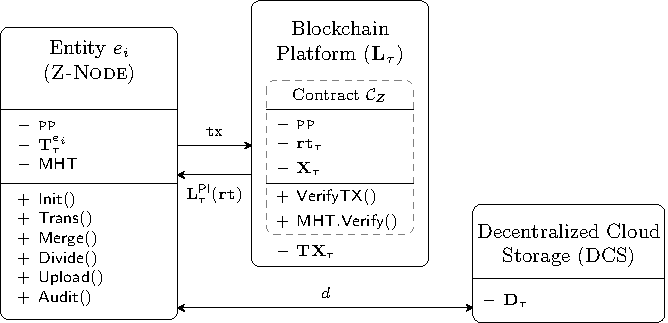
\includegraphics[width=0.8\linewidth]{Figures/Architecture}
    \caption[Primary components of the Zupply framework]{Primary components of the Zupply framework. In the figure, $\tau$ denotes time; \textsc{pp} represents public parameters; $\mathbf{T}_\tau^{e_i}$ denotes the set of \gls{aat}s associated with $e_i$; $\texttt{rt}_\tau$ is the root of the \textsf{MHT}; $\mathbf{X}_\tau$ is the set of \gls{aat}s that have reached their end-of-life (preventing re-transfer); \texttt{tx} denotes a transaction; $\mathbf{L}_\tau^\mathsf{PI}(\texttt{rt})$ is the proof-of-inclusion (PI) of $\texttt{rt}_\tau$ in the blockchain; $d$ denotes a data record; and $\mathbf{D}_\tau$ is the set of all such data records.}
    \label{fig:Zupply-Architecture}
\end{figure}

In the Zupply's \gls{dag} structure, data records are organized in sequences that can either split or merge. Except for the initial record, each one links back to its predecessor's \textsc{cid}. When sequences merge, they incorporate the \textsc{cid}s from previous records. Consequently, given any data record $d_n$, an auditor can trace back and retrieve all preceding records of $d_n$. This system allows any entity, such as a customer, to access a product's entire history up to that point by obtaining the most recent data record linked to the product, which could be uploaded by the last retailer in the chain. Given that the \textsc{cid} for each data record is derived from its multihash\footnote{Multihash is a self-identifying hash. It is a protocol designed to distinguish between the outputs of various established cryptographic hash functions \cite{multihash}.} \cite{Benet2014}, any modification to a record will invalidate the entire data sequence. 
% Also, each data record contains an encrypted section to ensure the confidentiality of sensitive information against public auditors. Appendix \ref{app:Data Encryption} suggests key management schemes to be employed in Zupply. 
Every data record comes with a \gls{zkp}, showing ownership of an \gls{aat} on the blockchain without revealing the owner's identity. Additionally, each record is digitally signed with a secret key, and the corresponding public key is a part of the \gls{aat}. 

In the initial stage of a supply chain (represented as a source vertex in a \gls{dag}), an \gls{aat} is created using the $\textsf{Init}$ algorithm, which is executed by the first entity. This token can then be passed along the supply chain to subsequent entities through \gls{aatot}, including three algorithms: $\textsf{Trans}$ for transferring the token, $\textsf{Merge}$ for combining two tokens before transferring, and $\textsf{Divide}$ for splitting a token into two tokens, which are then transferred. These processes, which employ \gls{zkp}s, not only ensure the token's continuous and secure progression through the supply chain but also preserve the unlinkability between entities. Entities within a supply chain can embed essential certificates into their data records to verify the product's originality to auditors. For instance, the initial data record could include a digital certificate of origin for a diamond, ensuring transparency and trust from the outset. However, subsequent entities responsible for transferring or storing the product can provide anonymous reports on conditions such as temperature, among others. These entities receive authorization to upload data from their predecessors, ensuring a secure and transparent chain of custody.

The Zupply Framework ensures that any entity uploading a data record has been authorized by its preceding entity. Therefore, it might be necessary for the first entity in a \gls{dag} to upload a certificate as a data record, allowing auditors to verify the source. This requirement remains indispensable in all \gls{scm} platforms, as customers check certificates issued by trusted certificate authorities, such as governments at the source or various steps of the supply chain. These certificates may or may not disclose the identity of the entities holding the certificates. In the initial stage of a \gls{dag}, the first \gls{aat} must be committed by an entity for its own use during the \textsf{Init} algorithm. While this process compromises the \gls{aat}'s anonymity, the authenticated data record will not reveal any information about the \gls{aat} itself. In contrast, the anonymity of owners for subsequently transferred tokens is maintained. This is because each \gls{aat} is committed by its preceding entity, ensuring the owner's anonymity. 


\subsection{Cryptographic Building Blocks}

Zupply utilizes the following cryptographic building blocks: 
\begin{enumerate}
    \item \textit{Statistically-hiding commitment} scheme (Definition \ref{def:Statistically-hiding commitment}) allows an entity to commit to their \gls{aat} $T$ by sending $\texttt{cm}:=\mathsf{COMM}_\rho(T)$ to the blockchain.

    \item \textit{Strongly-unforgeable digital signature} scheme (Definition \ref{def:Strongly-unforgeable digital signature}) is used for signing data records stored on \gls{dcs}.

    \item \textit{Symmetric-key encryption} scheme (Definition \ref{def:Symmetric-key encryption})  is used for encrypting the private part of data records.

    \item \textit{Zero-knowledge succinct non-interactive argument of knowledge} scheme (Definition \ref{def:zkSNARK Properties}) is used to ensure the authenticity of data records while preserving the anonymity of entities and unlinkability of \gls{aat} commitments.
\end{enumerate}


\subsection{Threat Model}

The adversary is driven by three primary motivations: the forgery or alteration of data records, the deanonymization of data uploaders, and the linking of collaborating entities. 

This adversary possesses the capability to access the blockchain, all data records stored on the \gls{dcs}, and observe all entities and their interactions with $\mathcal{C}_Z$. Zupply operates under the assumption that the adversary lacks possession of the product at each step of its lifecycle within the supply chain. This implies that they never hold an authentication token transferred from an authenticated entity. Therefore, any data reported by authorized entities, who are legitimately involved in the supply chain, is considered accurate. 

%A detailed discussion of the adversary's extensive assumptions, along with their objectives and potential attacks, is presented in Section \ref{sec:Attacker Model}.

\subsection{Security Goals}

The Zupply framework is designed as a trustless system for recording product histories, aiming to satisfy the following conditions:

\begin{enumerate}
\item The authenticity of data records, 
\item The integrity of data records,
\item The anonymity of data record uploaders and owners of transferred tokens,
\item The unlinkability among all entities collaborating within a supply chain.
\end{enumerate}


\subsection{Terms and Concepts in the Framework}
\label{sec:zupply-terms-and-concepts}
This section introduces the notations and symbols for data structures employed by Zupply. The symbol $\tau$ represents time and is also used to denote the state of each data structure. The superscript is for attribution, and the subscript is for indexing. For instance, \(T_i^{e_a}\) is the $i$th \gls{aat} which is attributed to or known by entity \(e_a\), while \(\texttt{tx}^{e_a}\) signifies that the transaction \(\texttt{tx}\) is published by \(e_a\) on the blockchain. Furthermore, to emphasize which entity runs a specific algorithm, the algorithm's name is presented as a superscript of the entity. For instance, if entity $e_a$ executes the algorithm \textsf{Init}, it is denoted as $e_a^\mathsf{Init}$.


\subsubsection{Entities}
\label{sec:Entities}
The set of all entities in Zupply is $\mathbf{E}_\tau = \{e_1, \dots, e_{|\mathbf{E}_\tau|}\}$. Each entity $e_i$, possesses a blockchain addresses denoted as $\text{BPAddr}^{e_i}$.  
This scheme operates without a central manager, placing all entities at an equal level of authority. Each entity runs the Zuppy Node (\textsc{Z-Node}).

\subsubsection{Anonymous Authentication Token (\gls{aat})}

For each \gls{aat} $T_i$  the keys $\text{SKsig}_{i}$ and $\text{PKsig}_{i}$ are generated using the key generation algorithm $\mathcal{K}_\mathsf{sig}$ based on a public key scheme, as defined in Definition~\ref{def:Strongly-unforgeable digital signature}.  Then, each \gls{aat} is represented as $T_i := (\Tilde{T}_i, \text{SKsig}_{i})$. Here $\Tilde{T}_i := (q_i, \text{PKsig}_{i}, \rho_i)$ denotes a partial \gls{aat}. Let $q_i \in \{0, 1\}^{N_q}$ keep track of the quantity of products, where ${N_q}$ is a  pre-determined security parameter which denotes the bit-length of quantity values in \glspl{aat}. It should be kept unchanged unless two supply chains are merged or one supply chain is divided into two sub supply chains. 

The owner of the \gls{aat} $T_i$ uses $\text{SKsig}_{i}$ to sign the data records uploaded by them. It is important not to confuse $\text{PKsig}_{i}$, which represents the public key associated with the token $T_i$, with the public keys related to the entity's $\text{BPAddr}$. 
Moreover, $\rho_i \in_R \{0, 1\}^{N_\rho}$, where ${N_\rho}$ is a  pre-determined security parameter which denotes the bit-length of $\rho$ values in \glspl{aat}, plays a crucial role in preventing the token's owner from re-transferring the \gls{aat} after transferring its ownership to the new owner(s). This is achieved by publishing the end-of-life (\gls{eol}) of the \gls{aat}, denoted as $\texttt{eol}_i = \mathcal{H}(\rho_i)$, on the blockchain. %Here, $\mathcal{H}$ represents a collision-resistant hash function. 
%\subsubsection{End of Life (\gls{eol})}
%In an \gls{aat}, $\rho_i \in_R \{0, 1\}^{N_\rho}$ prevents the owner of the \gls{aat} from re-transferring it after it has already been transferred by publishing the end-of-life (\gls{eol}), denoted as $\texttt{eol}_i = \mathcal{H}(\rho_i)$, on the blockchain.
$\mathbf{T}_\tau = \{T_1, \dots, T_{|\mathbf{T}_\tau|}\}$ denotes the time-ordered set of \gls{aat}s  and 
$\mathbf{X}_\tau = \{\texttt{eol}_1, \dots, \texttt{eol}_{|\mathbf{X}_\tau|}\}$ is the time-ordered set of published \gls{eol} of the obsoleted tokens. %We denote obsoleted token set at time $\tau$ as $\mathbf{O}_\tau$. Obsoleted tokens set is a subset of authentication tokens set $\mathbf{O}_\tau\subseteq \mathbf{T}_\tau$ for any $\tau$. 


\subsubsection{Commitment to \gls{aat}}
$\mathbf{C}_\tau = \{\texttt{cm}_1, \dots, \texttt{cm}_{|\mathbf{C}_\tau|}\}$ is the time-ordered set of commitments to $\mathbf{T}_\tau$. So, the corresponding commitment to  $T_i$ is denoted as $\texttt{cm}_i := \mathsf{COMM}_{\rho_i}(\Tilde{T_i})$. Figure \ref{fig:zupply-token} illustrates the diagram of committing to an \gls{aat}.




\begin{figure}
	\centering
	\includestandalone{Figures/TokenGenChart}
	\caption[Commitment to an Anonymous Authenticated Token]{The process of committing to an \gls{aat} and its corresponding \gls{eol}.}
	\label{fig:zupply-token}
\end{figure}


\subsubsection{Merkle Hash Tree}
Commitments to \gls{aat}s are stored on an $L$-layer Merkle hash tree ($|\mathbf{T}_\tau|<2^{L-1}$) denoted as $\mathsf{MHT}$ whose root is $\texttt{rt}_\tau$.
% The total number of anonymous authentication tokens is $|\mathbf{T}_\tau|<2^{L-1}$. 
Each leaf of $\mathsf{MHT}$ has an index number $ \mathsf{ind}\in [2^{L-1}]$ and $\mathsf{path}_\mathsf{ind}$ represents the Merkle proof corresponding to $\mathsf{ind}$. %The framework systematically populates the $\mathsf{MHT}$ following the order of the leaf indices. 
%A transition to the next state in the framework occurs if and only if one commitment is added to the $\mathsf{MHT}$. Consequently, $\texttt{rt}_\tau$ symbolizes the framework's state at time $\tau$. With this approach, we can define $\tau$ to be equivalent to the latest $\mathsf{ind}$, to which a commitment has been assigned. Moreover, $\mathsf{path}_\mathsf{ind}$ is the Merkle proof related to $\mathsf{ind}$.
$\mathsf{MHT}$ is a data structure that keeps the whole Merkle hash tree nodes and encompasses three algorithms: 
% $\mathsf{MHT}.\mathsf{Add}(\texttt{cm})$ is a stateful function which appends the new commitment to $\mathsf{MHT}$ and changes the \texttt{rt} accordingly. $\mathsf{MHT}.\mathsf{Verify}$ is a stateless function which verifies whether changing \texttt{rt} is consistent to the update of $\mathsf{MHT}$ (i.e., adding a new authentication token commitment to the tree): % The root of the Merkle tree (\texttt{rt}) is maintained $\mathsf{MHT}$ data structure. $\mathsf{MHT}$ has two methods:

\begin{enumerate} 

    \item $\mathsf{MHT}.\mathsf{Add}(\texttt{cm}) \rightarrow (\texttt{rt}^{\text{new}}, \mathsf{ind}, \mathsf{path}_\mathsf{ind})$. Given a new \texttt{cm},  the algorithm adds \texttt{cm} to the $\mathsf{MHT}$ and outputs the new Merkle root $\texttt{rt}^{\text{new}}$, the index of the new commitment ($\mathsf{ind}$), and $\mathsf{path}_\mathsf{ind}$.

    % \item $\mathsf{MHT}.\mathsf{Verify}(\texttt{cm}, \mathsf{path}) \rightarrow \{0, 1\}$. Given a commitment \texttt{cm} and Merkle path ($\mathsf{path}$),  $\mathsf{MHT}.\mathsf{Verify}$ outputs $1$ if \texttt{cm} is in $\mathsf{MHT}$, otherwise returns $0$.

    \item $\mathsf{MHT}.\mathsf{Verify}(\texttt{rt}_{\tau-1}, \texttt{rt}_{\tau}, \texttt{cm}, \mathsf{ind}, \mathsf{path}_\mathsf{ind})$ $ \rightarrow $ $\{0, 1\}$. Given the previous and the new root of $\mathsf{MHT}$ before and after assigning \texttt{cm} to the tree at  $\mathsf{ind}$, with corresponding $\mathsf{path}_\mathsf{ind}$, this algorithms verifies whether $\texttt{rt}_{\tau}$ is computed correctly.

    \item $\mathsf{MHT}.\mathsf{Search}(\texttt{cm}_i)$ $ \rightarrow $ $(\mathsf{ind}_i, \mathsf{path}_{\mathsf{ind}_i})$. Given  $\texttt{cm}_i$, $\mathsf{MHT}.\mathsf{Search}$ returns the index of  $\texttt{cm}_i$ ($\mathsf{ind}_i$), and the corresponding $\mathsf{path}_{\mathsf{ind}_i}$.
    
    % the previous and the new root of $\mathsf{MHT}$ before and after assigning \texttt{cm} to the leaf at the latest index  $\mathsf{ind} = \tau$ and the corresponding Merkle proof $\mathsf{path}_\mathsf{ind}$, this algorithms verifies whether $\texttt{rt}_{\tau}$ is consistent to $\texttt{rt}$ after this update or not.
\end{enumerate}

$\mathsf{MHT}.\mathsf{Add}()$ and $\mathsf{MHT}.\mathsf{Search}()$ are stateful, having direct access to the \textsf{MHT} data structure. In contrast, $\mathsf{MHT}.\mathsf{Verify}()$ does not. This algorithm is implemented within the smart contract, which does not store the \textsf{MHT}. %Detailed explanation of this algorithm is provided in Section \ref{sec:MerkleTreeStructure}.

\subsubsection{Blockchain Platform Ledger}
We can model the blockchain as an immutable, public, decentralized ledger, denoted as $\mathbf{L}_\tau$, on which the Zupply smart contract, $\mathcal{C}_Z$, is deployed.  $\mathcal{C}_Z$ maintains $\texttt{rt}_\tau$, and $\mathbf{X}_\tau$. The commitments in $\mathbf{C}_\tau$ are uploaded to the blockchain via transactions that invoke $\mathcal{C}_Z$. Consequently, $\mathbf{L}_\tau$ records all transactions associated with the Zupply framework (discussed below), along with other unrelated transactions on the blockchain platform.

Wherever data records are concerned, the protocol employs the \textit{proof-of-inclusion (\gls{pi})} mechanism provided by the blockchain to prove the correctness of the value $\texttt{rt}_\tau$ used in off-chain proofs. The PI of $\texttt{rt}_\tau$ in ledger $\mathbf{L}_\tau$ at time $\tau$ is represented as $\mathbf{L}_\tau^\mathsf{PI}(\texttt{rt})$. This proof ensures that the auditors can  verify  $\texttt{rt}$ employed for off-chain authentication.  

\subsubsection{Transactions}
Each transaction  $\texttt{tx}$ $\in$ $\{ \texttt{tx}_\textsf{Init},$ $\texttt{tx}_\textsf{Trans},$ $\texttt{tx}_\textsf{Merge},$ $\texttt{tx}_\textsf{Div} \}$ invokes a specific function in $\mathcal{C}_Z$. Each $\texttt{tx}$ contains one or two \texttt{cm}s, and whenever it finalizes on the blockchain,  its corresponding \texttt{cm}s are added to \textsf{MHT} locally and updates $\texttt{rt}_\tau$  on the blockchain. For a transactions that transfers the ownership of \gls{aat}(s), $\texttt{tx} \in \{$$\texttt{tx}_\textsf{Trans}$, $\texttt{tx}_\textsf{Merge}$, $\texttt{tx}_\textsf{Div}$ $\}$, the transaction contains the \gls{eol} of \gls{aat}(s) whose commitment(s) are stored on $\mathsf{MHT}$, and a \gls{zkp} of owning them. These proofs are denoted as $\pi_\mathbbm{x} \in \{\pi_\textsf{Trans}, \pi_\textsf{Merge}, \pi_\textsf{Div} \}$. The \gls{eol} should not be included in $\mathbf{X}_\tau$ prior to issuing the transaction. Only after the transaction is finalized by $\mathcal{C}_Z$, the smart contract updates $\mathbf{X}_\tau$ by adding the \gls{eol} to it.
% The transactions also contain the \textsf{BP} address of the transaction issuer, denoted as $\mathsf{BPAddr}^{e_i}$, which belongs to the entity $e_i$. 
The time-ordered set of transactions on blockchain is denoted as $\mathbf{TX}_\tau = \{\texttt{tx}_1, \dots, \texttt{tx}_{|\mathbf{TX}_\tau|}\}$.


% Zupply protocol employs an immutable public decentralized ledger denoted as $\mathbf{L}_\tau$ which keeps all the authentication token commitments ($\mathbf{C}_\tau$). The authentication token commitments are uploaded to the ledger via one the transactions $\texttt{tx}$ $\in$ $\{ \texttt{tx}_\textsf{Init}$$,$ $\texttt{tx}_\textsf{Trans}$$,$ $\texttt{tx}_\textsf{Merge}$$,$ $\texttt{tx}_\textsf{Div} \}$ which calls the Zupply smart contract $\mathcal{C}_Z$ deployed on the ledger. The smart contract maintains the value of the Merkle tree root $\texttt{rt}$. Wherever, specifically on data records, the protocol needs to prove the correctness of the value $\texttt{rt}$ on blockchain, it employs the \textit{proof-of-inclusion} provided by the blockchain platform. For example, Ethereum uses Merkle Patricia Trie \cite{PatriciaTree}. In this paper the poof-of-inclusion of $\texttt{rt}$ in ledger $\mathbf{L}_\tau$ is denoted as $\mathbf{L}_\tau(\texttt{rt})$.

\begin{figure}
	\centering
	\includestandalone[width=0.8\linewidth]{Figures/DataChain}
	% \includestandalone{./Figures/TokenGenChart}
	\caption[Data records in the Zupply framework]{Data records create a DAG structured data. $d_n$ represents the data record after two data sequences merges in the DAG.}
	\label{fig:zupply-datachain}
\end{figure}

\subsubsection{Data Records}
The time-ordered set of data records is denoted as $\mathbf{D}_\tau = \{d_1, \dots, d_{|\mathbf{D}_\tau|}\}$. Data records are stored on a \gls{dcs}. 
The \gls{cid} of a data record $d_n$ in the \gls{dcs} is denoted as $\textsc{cid}_n$.
The set of all \gls{cid}s is $\mathbf{CID}_\tau = \{\textsc{cid}_1, \dots, \textsc{cid}_{|\mathbf{CID}_\tau|}\}$. 
$\mathsf{DCS}(\textsc{cid}_n) \rightarrow d_n$ denotes a query to the \gls{dcs} to get the data record corresponded  \textsc{cid}.
% We can query the DCS to get the data record corresponded to each \textsc{cid}. The query is denoted as  $\mathsf{DCS}(\textsc{cid}_n) \rightarrow d_n$. %since each data record is corresponded to a content identifier, $|\mathbf{D}_\tau| = |\mathbf{CID}_\tau|$.
% Each data record $d_n$ is linked to two predecessor data records $d_p$ and $d_q$, where $p,q < n$. 
Each data record $d_n$ contains references to its predecessor, $d_p$ and $d_q$, where $p,q < n$, in the array $d_n.\mathsf{pred}$ if applicable. Specifically, $d_n.\mathsf{pred}[b] \in \mathbf{CID}_\tau$ for ${b = 0, 1}$; although one or both entries of the array may be $\emptyset$.
A data record $d_n$ contains public data $d_{n, \mathsf{pub}}$ which is stored as plain-text, and private data $d_{n, \mathsf{pri}}$ which is stored as cipher-text $c_n = \mathcal{E}_\mathsf{sym}(\textsc{k}_n, d_{n, \mathsf{pri}})$. Zupply may incorporate the forward secrecy scheme outlined in Mesh \cite{altawy2019mesh} to determine $\textsc{k}_n$ (Appendix \ref{app:Data Encryption}). $d_n$ also includes a \gls{zkp} $\pi_\textsf{Auth}$ of owning $T_i$ such that its corresponding $\texttt{cm}_i$ is in \textsf{MHT}.  The public input to this proof is denoted as $x_\texttt{Auth}$. Each $T_i$, can be used more than once to prove authenticity.
Also, the data record $d_n$ includes $\sigma_n = \mathcal{S}_\mathsf{sig}(\text{SKsig}_i, d_n)$, where $\text{SKsig}_i$ is the secret key associated with $\text{PKsig}_{i}$ in $T_i$. Consequently, $d_n$ is denoted as the following tuple and illustrated in Figure \ref{fig:zupply-datachain}:
\begin{align*}
    d_n  := & \left( d_{n, \mathsf{pub}}, c_n, \mathsf{pred}=\{\textsc{cid}_p, \textsc{cid}_q\}, \mathsf{tags}=\{\texttt{Tag}_p, \texttt{Tag}_q\}, \right. \\ 
    & \left. \pi_\textsf{Auth}, x_\textsf{Auth}=\{\texttt{rt}_\tau, \text{PKsig}_{i}\}, \mathbf{L}_\tau^\mathsf{PI}(\texttt{rt}_\tau) \right),
\end{align*}
where the digital signature $\sigma_n$  is uploaded together with the data  $d_n$ and the data ownership transfer tags (\textsf{tags}) are explained in the following.

\subsubsection{Data Ownership Transfer Tag} 
\label{sec:Data ownership transfer tag}

% The protocol enforces using data ownership transfer tag denoted as $\texttt{Tag}$ 
When two consecutive data records $d_{n-1}, d_n$ in a data sequence uses different secret keys for signing the data records. Namely, $\sigma_{n-1} = \mathcal{S}_\mathsf{sig}(\text{SKsig}_i, d_{n-1})$ and $\sigma_n = \mathcal{S}_\mathsf{sig}(\text{SKsig}_j, d_n)$. In this scenario, the later data record ($d_n$) has to include the $\texttt{Tag}_i = \mathcal{S}_\mathsf{sig}(\text{SKsig}_i, \text{PKsig}_j)$ created by the owner of the former data record ($d_{n-1}$). Data ownership transfer tags are created and used in \gls{aatot} presented in Section \ref{sec:Ownership Transfer}.


\subsubsection{Directed Acyclic Graph}
Given that each data record can reference its predecessor, they collectively form a DAG. Consequently, we define three key concepts integral to our DAG data structure:
\begin{enumerate}
    \item \textit{Init data ($d_{n, \mathsf{Init}}$)}: Any data record $d_n$ which does not have any predecessor, i.e., $d_n.\mathsf{pred}[b] = \emptyset$ for both ${b \in \{0, 1\}}$. %, initiates a new DAG. The data record $d_i$ is an \textit{Init} data record and denoted as $d_{i, \mathsf{Init}}$.

    \item \textit{Data Sequence ($S_k$)}: $S_k$ is a sequence of data records where each data record has one and only one predecessor. The first data record in $S_k$ can have zero, one, or two predecessors. %Namely, \textit{Data Sequence} $S_k$ is a time-ordered set of data records denoted as $S_k = \{d_{i_1}, \dots, d_{i_m}\}$ where $\forall n \in [2, m]$,  $d_{i_n}.\mathsf{pred}[0] = \textsc{cid}_{i_{n-1}}$, $d_{i_n}.\mathsf{pred}[1] =\emptyset$. 

    \item \textit{Progressive Data Sequence ($\hat{S}_k$)}: is a data sequence denoted as $\hat{S}_k = \{d_{i_1}, \dots, d_{i_m}\}$, where data record $d_{i_m}$ is the most recent, and it's ensured that no subsequent data record references $d_{i_m}$.

    % \item \textit{Forking Attack}: The potential attack to a data sequence is forking attack. For a data sequence $S_k$ such that $d_n \in S_k$, the adversary uploads a data 
\end{enumerate}






% \begin{remark} [\textsf{MHT} State-Related Algorithms]

% \end{remark}

\begin{remark} [\gls{aat} Public Key]
In the $\pi_\textsf{Auth}$, $\text{PKsig}$ is used as a public input. $\pi_\textsf{Auth}$ is then published off-chain on data records. However, for proofs directly published on the blockchain ($\pi_\textsf{Trans}$, $\pi_\textsf{Merge}$, and $\pi_\textsf{Div}$), $\text{PKsig}$ is treated as a private input. Also, the $\text{PKsig}$ is never published on blockchain. 
\end{remark}


\begin{definition}[Valid \gls{aat}]
	\label{def:Valid Authentication Token}
	$T_{i_2}$ is a valid \gls{aat} for authenticating a data record $d_{n_2}$ if and only if
	the $\texttt{cm}_{i_2} := \mathsf{COMM}_{\rho_{i_2}}(T_{i_2})$ is included in \textsf{MHT}.
\end{definition}


\begin{definition}[Authenticated Data]
	\label{def:Authenticated Data}
	A data record $d_{n}$ is an authenticated data if and only if $d_{n}$ contains
	\begin{enumerate}
		\item  a valid zero-knowledge proof of ($\pi_\texttt{Auth}$) of owning a \textit{valid \gls{aat}} $T_{i}$ (Definition \ref{def:Valid Authentication Token}).
		\item a valid signature $\sigma$ is created using the secret key $\text{SKsig}_{i}$, ensuring that both it and its corresponding public key $\text{PKsig}_{i}$ are included in $T_{i}$.
		\item valid tag(s) if and only if the predecessor data record is signed by different key(s) and $d_{n}.\text{pred} \neq \emptyset$
	\end{enumerate}
\end{definition}

\begin{definition}[Valid Transaction]
	\label{def:Valid Transaction}
	A transaction $\texttt{tx} $ $ \in $ $ \{ \texttt{tx}_\textsf{Init}, $ $ \texttt{tx}_\textsf{Trans}, $ $ \texttt{tx}_\textsf{Merge}, $ $ \texttt{tx}_\textsf{Div} \}$ is a valid transaction if and only if
	\begin{enumerate}
		\item $\mathsf{MHT}.\mathsf{Verify}(\texttt{rt}_{\tau}, \texttt{rt}^\text{new}, \texttt{cm}, \mathsf{ind}, \mathsf{path}_\mathsf{ind}) = 1$, where The root of \textsf{MHT} was $\texttt{rt}_{\tau}$ before $\texttt{tx}$. For $\textsf{Div}$ transaction (i.e., $\texttt{tx}= \texttt{tx}_\textsf{Div}$) the transition of the root is examined in two rounds of running $\mathsf{MHT}.\mathsf{Verify}$ algorithm: $\texttt{rt}_\tau \rightarrow \texttt{rt}^\text{new}_1 \rightarrow \texttt{rt}^\text{new}_2$. 
		
		
		\item $\texttt{eol} \notin  \mathbf{X}_\tau$. Where $\texttt{tx}_\mathsf{Trans}$ and $\texttt{tx}_\mathsf{Div}$ contain one and $\texttt{tx}_\mathsf{Merge}$ contains two \texttt{eol}s. This value represents the \gls{aat} that is expired during the owner transferring algorithms.
		
		\item $\mathsf{Verify}(\text{vk}_\mathbbm{x}, x_\mathbbm{x}, \pi_\mathbbm{x}) = 1$ for $\mathbbm{x} \in \{\mathsf{Trans}$, $\mathsf{Merge}$, $\mathsf{Div} \}$
		
	\end{enumerate}
\end{definition}




\subsection{NP Statements}
\label{sec:Zero-knowledge Proofs}
This section presents the \gls{np}-statements related to \gls{zkp}s employed in Zupply. 


\subsubsection{Authenticity proof ($\pi_\textsf{Auth}$)}
Whenever an entity wants to upload a data record on DCS, the entity (prover) proves they own a commitment \texttt{cm} in the \textsf{MHT}. The \gls{np} problems associated with this proof are explained as follows:

    
\begin{itemize}

    \item $\texttt{cm}_i =\mathsf{COMM}_{\rho_i}(\Tilde{T}_i)$
	\item $\texttt{path}_i$ is a valid path from leaf  $\texttt{cm}_i$ to root $\texttt{rt}_\tau$.
\end{itemize}

Where $\Tilde{T}_i = (q_i, \text{PKsig}_i, \rho_i)$. To prove that the used \texttt{rt} is a valid value stored on $\mathcal{C}_Z$, the entity provides the \gls{pi} $\mathbf{L}_\tau^\mathsf{PI}(\texttt{rt})$.



\subsubsection{Transferability proof ($\pi_\textsf{Trans}$)}

When an entity wishes to transfer the ownership of an \gls{aat} ($T_{i_1}$), it (as the prover) proves that the newly minted $\Tilde{T}_{i_2}$ maintains the same product quantity as $T_{i_1}$ (i.e., $q_{i_1} = q_{i_2}$), without disclosing details about $T_{i_1}$ and $\Tilde{T}_{i_2}$. Moreover,  $\texttt{cm}_{i_1}$ is kept confidential. In addition, the entity proves that the published $\texttt{eol}_{i_1}$ is equal to $\mathcal{H}(\rho_{i_1})$, while keeping $\rho_{i_1}$ secret. The \gls{np} problems associated with this proof are explained as follows:

\begin{itemize}
	\item $\texttt{eol}_{i_1} = \mathcal{H}(\rho_{i_1} )$
	\item $\texttt{cm}_{i_1} = \mathsf{COMM}_{\rho_{i_1}}(\Tilde{T}_{i_1})$
	\item $\texttt{path}_{{i_1}}$ is a valid path from leaf  $\texttt{cm}_{\texttt{cm}_{i_1}}$ to root $\texttt{rt}_\tau$
	\item $\texttt{cm}_{i_2} = \mathsf{COMM}_{\rho_{i_2}}(\Tilde{T}_{i_2})$
	\item $q_{i_1} = q_{i_2} $
\end{itemize}
Where  $\Tilde{T}_{i_1} = (q_{i_1}, \text{PKsig}_{i_1}, \rho_{i_1})$, $\Tilde{T}_{i_2} = (q_{i_2}, \text{PKsig}_{i_2}, \rho_{i_2})$, and $x_\mathsf{Trans} = (\texttt{eol}_{i_1}, \texttt{cm}_{i_2}, \texttt{rt}_\tau)$ denotes the public inputs.

\subsubsection{Mergeability proof ($\pi_\textsf{Merge}$)}
An entity may merge two \gls{aat}s $T_{i_1}$ and $T_{i_2}$ to create $T_{i_3}$. The entity proves that the quantity in $T_{i_3}$ is the same as the summation of quantities in $T_{i_1}$ and $T_{i_2}$ (i.e., $q_{i_1} + q_{i_2} = q_{i_3}$).  The \gls{zkp} $\pi_\mathsf{Merge}$ follows the same approach as $\pi_\mathsf{Trans}$. The \gls{np} problems associated with this proof are explained as follows:
\begin{itemize}
    \item $\texttt{eol}_{i_1} = \mathcal{H}(\rho_{i_1} )$ and $\texttt{eol}_{i_2} = \mathcal{H}(\rho_{i_2} )$
	\item $\texttt{cm}_{i_1} = \mathsf{COMM}_{\rho_{i_1}}(\Tilde{T}_{i_1})$, $\texttt{cm}_{i_2} = \mathsf{COMM}_{\rho_{i_2}}(\Tilde{T}_{i_2})$

	\item $\texttt{path}_{{i_1}}$ and $\texttt{path}_{{i_2}}$  are valid paths respectively from leaf  $\texttt{cm}_{\texttt{cm}_{i_1}}$  and 
      $\texttt{cm}_{\texttt{cm}_{i_2}}$ to root $\texttt{rt}_\tau$.

    \item $\texttt{cm}_{i_3} = \mathsf{COMM}_{\rho_{i_3}}(\Tilde{T}_{i_3})$
	\item $q_{i_1} + q_{i_2} = q_{i_3} $
    
\end{itemize}
Where  $\Tilde{T}_{i_1} = (q_{i_1}, \text{PKsig}_{i_1}, \rho_{i_1})$, $\Tilde{T}_{i_2} = (q_{i_2}, \text{PKsig}_{i_2}, \rho_{i_2})$ and $\Tilde{T}_{i_3} = (q_{i_3}, \text{PKsig}_{i_3}, \rho_{i_3})$.
The public input to the proof is denoted as $x_\mathsf{Merge} = (\texttt{eol}_{i_{1,2}}, \texttt{cm}_{i_3}, \texttt{rt}_\tau)$.


\subsubsection{Divisibility proof ($\pi_\textsf{Div}$)}
An entity can divide an \gls{aat} $T_{i_1}$ into two new ${T}_{i_2}$ and ${T}_{i_3}$. The approach of creating \gls{zkp} $\pi_\textsf{Div}$ follows the same approaches in $\pi_\textsf{Trans}$ and $\pi_\textsf{Merge}$. The \gls{np} problems associated with this proof are explained as follows:

\begin{itemize}
    \item $\texttt{eol}_{i_1} = \mathcal{H}(\rho_{i_1} )$
	\item $\texttt{cm}_{i_1} = \mathsf{COMM}_{\rho_{i_1}}(\Tilde{T}_{i_1})$
	\item $\texttt{path}_{{i_1}}$ is a valid path from leaf  $\texttt{cm}_{\texttt{cm}_{i_1}}$ to root $\texttt{rt}_\tau$


    \item $\texttt{cm}_{i_2} = \mathsf{COMM}_{\rho_{i_2}}(\Tilde{T}_{i_2})$ and $\texttt{cm}_{i_3} = \mathsf{COMM}_{\rho_{i_3}}(\Tilde{T}_{i_3})$
	\item $q_{i_1} = q_{i_2} + q_{i_3}$
    
\end{itemize}
Where  $\Tilde{T}_{i_1} = (q_{i_1}, \text{PKsig}_{i_1}, \rho_{i_1})$, $\Tilde{T}_{i_2} = (q_{i_2}, \text{PKsig}_{i_2}, \rho_{i_2})$ and $\Tilde{T}_{i_3} = (q_{i_3}, \text{PKsig}_{i_3}, \rho_{i_3})$. The public input is denoted as $x_\mathsf{Div} =\big(\texttt{eol}_{i_1}, \texttt{cm}_{i_{2,3}}, \texttt{rt}_\tau \big)$.

\section{Zupply Algorithms and Protocols}
\label{sec:Zupply Algorithms}
The Zupply framework comprises a set of  algorithms and protocols detailed in Sections \ref{sec:Zupply-Algorithms} and \ref{sec:Zupply-Protocols}, respectively.

\begin{definition}[Zupply Framework]
\label{def:Zupply Framework}
Zupply framework $\Pi$ Consists of a tuple of polynomial-time algorithms and protocols $\Pi = $ ($\textsf{Setup}$, $\textsf{Init}$,  $\textsf{Trans}$, $\textsf{Merge}$, $\textsf{Divide}$, $\textsf{Upload}$, $\textsf{VerifyTX}$, $\textsf{Audit}$; $\textsf{OT-Protocol}$, $\textsf{MHT-Protocol}$).
\end{definition}



\subsection{Algorithms} \label{sec:Zupply-Algorithms}%
% Using security parameter $\lambda$, we define Zupply Scheme. // explain $i$
All algorithms have read-only access to $\mathbf{TX}\tau$, $\mathbf{C}\tau$, \textsf{MHT}, $\mathbf{X}\tau$, and $\mathbf{D}\tau$ (accessible via \textsf{DCS} queries). The smart contract is responsible for updating $\mathbf{TX}\tau$, $\mathbf{C}\tau$, $\mathbf{X}_\tau$, and the root of \textsf{MHT} when the \textsf{VerifyTX} algorithm outputs 1.

\subsubsection{\textsf{Setup} ($1^{\lambda}$) $\rightarrow$ $\textsc{pp}$}
Given a security parameter $\lambda$, \textsf{Setup} generates a set of global public parameters, denoted as \textsc{pp}. The specific implementation of \textsf{Setup} depends on the \gls{zksnark} algorithm in use: it may require a trusted party, or it may rely on a transparent (public) setup. The resulting \textsc{pp} is made publicly available. The pseudocode for \textsf{Setup} is provided in Algorithm~\ref{alg:Setup}.

%%%%%%%%%%%%%%%%%%%%%%%%%% Setup %%%%%%%%%%%%%%%%%%%%%%%%%%
\begin{algorithm}[h]
\caption{\textsf{Setup} ($1^{\lambda}$) $\rightarrow$ $\textsc{pp}$ }\label{alg:Setup}
\begin{algorithmic}

\State $(\text{pk}_\texttt{Auth}, \text{vk}_\texttt{Auth}) \leftarrow \textsf{KeyGen}(1^{\lambda}, \mathsf{Auth})$ 

\State $(\text{pk}_\textsf{Trans}, \text{vk}_\textsf{Trans}) \leftarrow \textsf{KeyGen}(1^{\lambda}, \mathsf{Trans})$ 

\State $(\text{pk}_\textsf{Merge}, \text{vk}_\textsf{Merge}) \leftarrow \textsf{KeyGen}(1^{\lambda}, \mathsf{Merge})$ 

\State $(\text{pk}_\textsf{Div}, \text{vk}_\textsf{Div}) \leftarrow \textsf{KeyGen}(1^{\lambda}, \mathsf{Divide})$ 

\State $\textsc{pp}_\mathsf{sig} \leftarrow \mathcal{G}_\mathsf{sig}(1^{\lambda})$


\State $\textsc{pp}$ $\leftarrow$ $($$\text{pk}_\texttt{Auth}$, $\text{vk}_\texttt{Auth}$, $\text{pk}_\textsf{Trans}$, $\text{vk}_\textsf{Trans}$, $\text{pk}_\textsf{Merge}$, $\text{vk}_\textsf{Merge}$, $\text{pk}_\texttt{Div}$, $\text{vk}_\texttt{Div}$, $\textsc{pp}_\mathsf{sig}$ $)$

\State \Return $\textsc{pp}$

\end{algorithmic}
\end{algorithm}
% ###########################################


\subsubsection{\textsf{Init} ($\textsc{pp}$, $q_{i_1}$) $\rightarrow$ ($\texttt{tx}_{\textsf{Init}}$, $T_{i_1}$) }
Initiates a \gls{dag}. The algorithm gets $q_{i_1}$, which will be maintained in the \gls{dag}. It creates a new token $T_{i_1}$, commits to it, and sends the commitment via
 \[
 \texttt{tx}_{\mathsf{Init}} := (\texttt{cm}_{i_1}, \texttt{rt}^{\text{new}}, \mathsf{ind}_{i_1}, \mathsf{path}_{\mathsf{ind}_{i_1}})
 \]
 to the blockchain. The pseudocode for \textsf{Init} is provided in Algorithm~\ref{alg:Init} is provided in Algorithm~\ref{alg:trans} in Appendix \ref{a_ch:zupply_algorithms}.



\subsubsection{\textsf{Trans} (\textsc{pp}, $T_{i_1}$,  $\text{PKsig}_{i_2}$) $\rightarrow$ ($\texttt{tx}_{\textsf{Trans}}$, $\Tilde{T}_{i_2}$, $\texttt{Tag}$)}

This algorithm takes an existing \gls{aat} $T_{i_1}$ and renders it obsolete by publishing its associated \gls{eol} on the blockchain. Specifically, it computes $\texttt{eol}_{i_1} := \mathcal{H}(\rho_{i_1})$, where $\rho_{i_1}$ is a secret contained in $T_{i_1}$, and includes this value in the resulting transaction $\texttt{tx}_{\textsf{Trans}}$.
Subsequently, the algorithm constructs a new partial \gls{aat}, denoted $\Tilde{T}_{i_2}$, by sampling a fresh random value $\rho_{i_2}$ and assigning it the same quantity as in $T_{i_1}$. The public key $\text{PKsig}_{i_2}$ is used to bind the new token to its intended recipient, in accordance with the \textsf{OT-Protocol} described in Section~\ref{sec:Ownership Transfer}. The algorithm commits to $\Tilde{T}_{i_2}$ and includes the resulting commitment in the transaction.
The transaction also includes a \gls{zkp} demonstrating:
(1)  knowledge of $T_{i_1}$ whose commitment is included in the \textsf{MHT}, without revealing the commitment itself,
(2) consistency of this committment with the published $\texttt{eol}_{i_1}$,
(3) knowledge of the preimage of the new commitment ($\texttt{cm}_{i_2}$) to $\Tilde{T}_{i_2}$, and
(4) equality of the quantity values in $T_{i_1}$ and $\Tilde{T}_{i_2}$.
Accordingly, the contents of the transaction $\texttt{tx}_{\textsf{Trans}}$ are defined as:
\[
\texttt{tx}_{\textsf{Trans}} := \big(\pi_{\textsf{Trans}}, x_{\textsf{Trans}}, \texttt{eol}_{i_1}, \texttt{cm}_{i_2}, \texttt{rt}^{\text{new}}, \mathsf{ind}_{i_2}, \mathsf{path}_{\mathsf{ind}_{i_2}} \big)
\]
where 
\[
x_\textsf{Trans} := \big(\texttt{eol}_{i_1}, \texttt{cm}_{i_2}, \texttt{rt}_\tau \big)
\]
denotes the public inputs to the \gls{zkp}, $\texttt{rt}^{\text{new}}$ is the updated root of the \textsf{MHT} after inserting the new commitment $\texttt{cm}_{i_2}$, and $\mathsf{ind}_{i_2}$ with $\mathsf{path}_{\mathsf{ind}{i_2}}$ represent the index and Merkle proof of the new commitment.
Finally, the algorithm outputs a $\texttt{Tag}$, which enables the new \gls{aat} owner to continue the data sequence, ensuring continuity with the most recent data record generated using $T_{i_1}$. The pseudocode for \textsf{Trans} is provided in Algorithm~\ref{alg:trans} in Appendix~\ref{a_ch:zupply_algorithms}.




\subsubsection{\textsf{Merge} (\textsc{pp}, $T_{i_{1}}$, $T_{i_{2}}$,  $\text{PKsig}_{i_3}$) $\rightarrow$ ($\texttt{tx}_{\textsf{Merge}}$, $\Tilde{T}_{i_3}$, $\texttt{Tag}_{i_{1}}$, $\texttt{Tag}_{i_{2}}$)}

The \textsf{Merge} algorithm follows a similar approach to the \textsf{Trans} algorithm. In this procedure, two \glspl{aat}, $T_{i_1}$ and $T_{i_2}$, are rendered obsolete, and their corresponding \glspl{eol}, $\texttt{eol}_{i_{1}}$ and $\texttt{eol}_{i_{2}}$, are published to the blockchain via $\texttt{tx}_{\textsf{Merge}}$. A new partial token, $\Tilde{T}_{i_3}$, is created using the input public key $\text{PKsig}_{i_3}$, sampling a random value $\rho_{i_2}$, and a quantity value set to the sum of the quantity values in $T_{i_1}$ and $T_{i_2}$.
The transaction also includes a commitment to the new \gls{aat}, denoted by $\texttt{cm}_{i_3}$, along with a \gls{zkp} that proves the following statements without revealing the underlying values: (1) knowledge of $T_{i_1}$ and $T_{i_2}$ whose commitments are included in the \textsf{MHT}, (2)  consistency of these commitments with the published $\texttt{eol}_{i_{1}}$ and $\texttt{eol}_{i_{2}}$, (3) the knowledge of $\Tilde{T}{i_3}$ in the new commitment $\texttt{cm}_{i_3}$ to $\Tilde{T}_{i_3}$, and (4) that the quantity in $\Tilde{T}_{i_3}$ equals the sum of the quantities in $T_{i_1}$ and $T_{i_2}$.  Accordingly, the transaction $\texttt{tx}_{\textsf{Merge}}$ is defined as:
\[
\texttt{tx}_\mathsf{Merge} :=(\pi_{\mathsf{Merge}}, x_\mathsf{Merge}, \texttt{eol}_{i_{1}}, \texttt{eol}_{i_{2}},  \texttt{cm}_{i_3}, \texttt{rt}^{\text{new}}, \mathsf{ind}_{i_3}, \mathsf{path}_{\mathsf{ind}_{i_3}}),
\]
where
\[
x_\mathsf{Merge} = (\texttt{eol}_{i_{1}}, \texttt{eol}_{i_{2}} \texttt{cm}_{i_3}, \texttt{rt}_\tau)
\]
denotes the public inputs to the \gls{zkp}. Here, $\texttt{rt}_1^{\text{new}}$ is the updated root of the \textsf{MHT} after inserting the first new commitment $\texttt{cm}_{i_2}$, and $\texttt{rt}_2^{\text{new}}$ is the root after inserting the second new commitment $\texttt{cm}_{i_3}$. Accordingly, $\mathsf{ind}_{i_2}$ with its corresponding Merkle path $\mathsf{path}_{\mathsf{ind}_{i_2}}$, and $\mathsf{ind}_{i_3}$ with $\mathsf{path}_{\mathsf{ind}_{i_3}}$, represent the indices and Merkle proofs for the first and second new commitments, respectively.
The \textsf{Merge} algorithm also outputs two data ownership transfer tags, $\texttt{Tag}_{i_{1}}$ and $\texttt{Tag}_{i_{2}}$, which are used together in a new data record to ensure continuity with the two most recent data records generated by the \glspl{aat} $T_{i_1}$ and $T_{i_2}$ and merging those sequences. The pseudocode for the \textsf{Merge} algorithm is provided in Algorithm~\ref{alg:merge} in Appendix~\ref{a_ch:zupply_algorithms}.

%Obsoletes $T_{i_1}$, $T_{i_2}$ and generates $\Tilde{T}_{i_3}$ ($q_{i_3} = q_{i_1} + q_{i_2}$).  $T_{i_1}$, $T_{i_2}$, $\Tilde{T}_{i_3}$, $\texttt{cm}_{i_1}$, and $\texttt{cm}_{i_2}$ are not disclosed. $\texttt{tx}_\mathsf{Merge} $:$=(\pi_{\mathsf{Merge}}, x_\mathsf{Merge}, \texttt{eol}_{i_{1,2}},  \texttt{cm}_{i_3}, \texttt{rt}^{\text{new}}, \mathsf{ind}_{i_3}, \mathsf{path}_{\mathsf{ind}_{i_3}} )$,
% where $x_\mathsf{Merge} = (\texttt{eol}_{i_{1,2}}, \texttt{cm}_{i_3}, \texttt{rt}_\tau)$.



\subsubsection{\textsf{Divide} ($\textsc{pp}$, $T_{i_1}$,  $\text{PKsig}_{i_{2}}$, $\text{PKsig}_{i_{3}}$, $q_{i_{2}}$, $q_{i_{3}}$) $\rightarrow$ ($\texttt{tx}_{\textsf{Div}}$, $\Tilde{T}_{i_{2}}$, $\Tilde{T}_{i_{3}}$, $\texttt{Tag}_{i_{2}}$, $\texttt{Tag}_{i_{3}}$)}

The \textsf{Divide} algorithm is the inverse of the \textsf{Merge} algorithm. It takes a single \gls{aat}, $T_{i_1}$, as input and creates two new partial \glspl{aat}, denoted $\Tilde{T}_{i_2}$ and $\Tilde{T}_{i_3}$. These are generated using the provided public keys $\text{PKsig}_{i_2}$ and $\text{PKsig}_{i_3}$, sampled random values $\rho_{i_2}$ and $\rho_{i_3}$, and quantity values $q_{i_2}$ and $q_{i_3}$, such that the sum $q_{i_2} + q_{i_3}$ equals the quantity in $T_{i_1}$. 
This algorithm renders $T_{i_1}$ obsolete, and its associated \gls{eol}, denoted $\texttt{eol}_{i_1}$, is included in the transaction sent to the blockchain. The transaction also includes the commitments to the newly created partial tokens, $\texttt{cm}_{i_2}$ and $\texttt{cm}_{i_3}$, as well as a \gls{zkp} proving the following statements: (1) knowledge of $T_{i_1}$, whose commitment is included in the \textsf{MHT}, (2) consistency between the commitment to $T_{i_1}$ and the published $\texttt{eol}_{i_1}$, (3)  knowledge of $\Tilde{T}_{i_2}$ and $\Tilde{T}_{i_3}$ which are the preimages of the commitments $\texttt{cm}{i_2}$ and $\texttt{cm}{i_3}$, and (4)  that the quantity in $T_{i_1}$ equals the sum of the quantities in $\Tilde{T}_{i_2}$ and $\Tilde{T}_{i_3}$.
Accordingly, the transaction $\texttt{tx}_{\textsf{Div}}$ is defined as:
\[
\texttt{tx}_\mathsf{Div} :=(\pi_{\mathsf{Div}}, x_\mathsf{Div}, \texttt{eol}_{i_{1}},  \texttt{cm}_{i_{2}}, \texttt{cm}_{i_{3}}, \texttt{rt}_{1}^{\text{new}}, , \texttt{rt}_{2}^{\text{new}}, \mathsf{ind}_{i_{2}}, \mathsf{ind}_{i_{3}}, \mathsf{path}_{\mathsf{ind}_{i_{2}}}, \mathsf{path}_{\mathsf{ind}_{i_{3}}} )
\]
where
\[
x_\mathsf{Div} =\big(\texttt{eol}_{i_1}, \texttt{cm}_{i_{2}}, \texttt{cm}_{i_{3}}, \texttt{rt}_\tau \big)
\]
denotes the public inputs to the \gls{zkp}.  The algorithm also outputs two data ownership transfer tags, $\texttt{Tag}_{i_2}$ and $\texttt{Tag}_{i_3}$, which are used in two separate data records whose common predecessor is the most recent data record generated by $T_{i_1}$. Each resulting data record initiates a new data sequence.  The pseudocode for the \textsf{Divide} algorithm is provided in Algorithm~\ref{alg:divide} in Appendix~\ref{a_ch:zupply_algorithms}.

%Obsoletes $T_{i_1}$ and generates $\Tilde{T}_{i_2}$ and $\Tilde{T}_{i_3}$ ($q_{i_1} = q_{i_2} + q_{i_3}$). $T_{i_1}$, $\Tilde{T}_{i_2}$, $\Tilde{T}_{i_3}$, and  $\texttt{cm}_{i_1}$ are not disclosed. $\texttt{tx}_\mathsf{Div} $:$=(\pi_{\mathsf{Div}}, x_\mathsf{Div}, \texttt{eol}_{i_{1}},  \texttt{cm}_{i_{2,3}}, \texttt{rt}_{1,2}^{\text{new}},\mathsf{ind}_{i_{2,3}}, \mathsf{path}_{\mathsf{ind}_{i_{2,3}}} )$, where $x_\mathsf{Div} =\big(\texttt{eol}_{i_1}, \texttt{cm}_{i_{2,3}}, \texttt{rt}_\tau \big)$.





\subsubsection{\textsf{VerifyTX} (\textsc{pp}, $\texttt{tx}_\mathbbm{x}$) $\rightarrow$ $b \in \{0, 1\}$}

The \textsf{VerifyTX} algorithm is executed within the Zupply smart contract $\mathcal{C}_Z$.
It takes as input a transaction $\texttt{tx}$ and returns one if and only if $\texttt{tx}$ is valid, as defined in Definition~\ref{def:Valid Transaction}. Below, we present the algorithm in more detail.

The verification steps depend on the type of transaction, denoted by $\mathbbm{x}$, which can be one of \textsf{Trans}, \textsf{Merge}, or \textsf{Div}. Regardless of the type, the algorithm ensures that the \gls{eol} in the transaction is not included in the set $\mathbf{X}_\tau$. It also calls the \textsf{MHT}.\textsf{Verify} algorithm (described in Algorithm~\ref{alg:ٰMHTVerify}) to check whether the proposed updated Merkle root $\texttt{rt}^\textsf{new}$ has been computed correctly, following the \textsf{MHT-Protocol}, which is introduced later.  Note that the smart contract does not store the \textsf{MHT} itself.
Furthermore, the \glspl{zkp} corresponding to each transaction type, $\pi_\mathsf{Trans}$, $\pi_\mathsf{Merge}$, and $\pi_\mathsf{Div}$, are verified using their respective verification keys, namely $\mathsf{vk}_\mathsf{Trans}$, $\mathsf{vk}_\mathsf{Merge}$, and $\mathsf{vk}_\mathsf{Div}$, along with the public inputs embedded in the transaction.

In addition to the shared verification logic, \texttt{tx} of type \textsf{Merge} includes one extra \gls{eol} element that must also be checked for exclusion from $\mathbf{X}_\tau$. On the other hand, a \textsf{Div} transaction includes two new commitments, requiring an additional verification step. After verifying the first new Merkle root as described, the algorithm verifies the second root against the second commitment.

If any of these verifications fail, the algorithm returns zero. Otherwise, it returns one.
The pseudocode for \textsf{VerifyTX} is provided in Algorithm~\ref{alg:divide} in Appendix~\ref{a_ch:zupply_algorithms}.


\subsubsection{\textsf{Upload} ($\textsc{pp}$, $[\textsf{pred}]$, $T_i$, $d_{\mathsf{pub}}$, $d_{\mathsf{pri}}$, $\textsc{k}_{n_3}$, $[\textsf{tags}]$) $\rightarrow$ $d_{n_3}$}

The \textsf{Upload} algorithm processes components of $d_{n_3}$ along with the \textsc{cid} of the predecessor data records and the corresponding data ownership transfer tags, if applicable. 

The algorithm commits to the \gls{aat} $T_i$ provided as input and searches for the corresponding commitment in the \textsf{MHT}. Once the commitment is located, it generates a \gls{zkp}, denoted as $\pi_\mathsf{Auth}$, that proves knowledge of a pre-image to a commitment in the \textsf{MHT}. Unlike the \glspl{zkp} generated by other algorithms, this proof includes $\text{PKsig}_i$, which is embedded in $T_i$, as a public input to the proof.
This inclusion is essential because, once all components of the new data record $d_{n_3}$ are generated, the record is signed using the $\text{SKsig}_i$ found in $T_i$. The presence of $\text{PKsig}_i$ as a public input allows the verifier to validate the signature and ensures that the same $T_i$ (which includes $\text{PKsig}_i$) was used throughout the sequence. If a different \gls{aat} were substituted in the sequence, the \textsf{Audit} algorithm, described later, would reject the data record, as it detects a mismatch in the $\text{PKsig}$ relative to previous records. An exception to this rule occurs only when a data ownership transfer tag is included in the first data record that uses a different \gls{aat}. Such a tag is generated by one of the \textsf{Trans}, \textsf{Merge}, or \textsf{Divide} algorithms. 

The public input to the aforementioned \gls{zkp} includes the Merkle root at the time the proof is generated, denoted as $\texttt{rt}_\tau$. Since auditors are lightweight clients and do not store the blockchain, they cannot directly verify whether the claimed $\texttt{rt}_\tau$ is indeed the Merkle root of the \textsf{MHT}. To address this, the prover includes $\mathbf{L}_\tau^\mathsf{PI}(\texttt{rt}_\tau)$, a proof that attests to the correctness of $\texttt{rt}_\tau$ on the blockchain. This proof is constructed in a manner that allows verification by lightweight clients. 

Moreover, given the secret key $\textsc{k}_{n_3}$ and the private portion of the data record, denoted as $d_\text{pri}$, the \textsf{Upload} algorithm encrypts $d_\text{pri}$ using $\textsc{k}_{n_3}$. The pseudocode for \textsf{Upload} is provided in Algorithm~\ref{alg:Upload} in Appendix~\ref{a_ch:zupply_algorithms}.




\subsubsection{\textsf{Audit} ($\textsc{pp}$, $d_n$) $\rightarrow$ $b \in \{0, 1\}$}

The \textsf{Audit} algorithm takes a data record \(d_{n}\) and returns one if and only if it is an authenticated data record, as specified in Definition~\ref{def:Authenticated Data}. More precisely, it verifies the \gls{zkp} included in \(d_n\), and checks the correctness of \(\texttt{rt}_\tau\) using \(\mathbf{L}_\tau^\mathsf{PI}(\texttt{rt}_\tau)\).

If the set of predecessor data records \(\textsf{pred}\) is non-empty, the algorithm retrieves each predecessor and checks whether they share the same \text{PK{sig}}. Otherwise, \(d_n\) must include a data ownership transfer tag, which consists of the \text{PK{sig}} in \(d_n\) signed by the key that signed the predecessor data record. The \textsf{Audit} algorithm then verifies the signature in \(d_n\) as well as the data ownership transfer tags, if present. The pseudocode for \textsf{Audit} is provided in Algorithm~\ref{alg:Audit} in Appendix~\ref{a_ch:zupply_algorithms}.



\subsection{Protocols}
\label{sec:Zupply-Protocols}

\subsubsection{Ownership Transfer (\textsf{OT-Protocol})}
\label{sec:Ownership Transfer}

Let \textit{A} and \textit{B} be two consecutive entities within a supply chain. \textit{A} (the transferor) wants to transfer $T^A_1$ to \textit{B} (the transferee). They communicate via an off-chain secure channel, which can be realized in multiple ways, such as through their in-person interaction during the product transfer. First, \textit{A} requests \textit{B} for a new $\text{PKsig}^B_2$. Then, passes $T^A_1$ and $\text{PKsig}^B_2$ to the \textsf{Trans} algorithm to generate $\Tilde{T}^B_2$ and $\texttt{Tag}_1$. Then, gives them to \textit{B}. Subsequently, \textit{B} samples  new pairs of $\text{PKsig}^B_3$ and $\text{SKsig}^B_3$ and runs the \textsf{Trans} again to obsolete the received \gls{aat} ($\Tilde{T}^B_2$) and create $\Tilde{T}^B_3$. This preserves the privacy of the lifecycle of the transferred \gls{aat} from \textit{A}, who can determine when the \gls{aat} $T_2^B$ is transferred since \textit{A} knows $\rho_2^B$. However, \textit{A} cannot discern if, when and to whom $T_3^B$ is transferred. Also, entities not involved cannot recognize a link between the corresponding \gls{aat} commitments, i.e., $\texttt{cm}^A_1$, $\texttt{cm}^B_2$, $\texttt{cm}^B_3$. Additionally, for merging and dividing, \textit{A} runs \textsf{Merge} or \textsf{Divide} locally, then transfers the outputted token(s) using the explained protocol.Figure \ref{fig:Ownership Transfer} describes the protocol.

\begin{figure}[h]
    \centering
    {
    \includestandalone[width=\linewidth]{Figures/Ownership_Transformation}
    }
    \vspace{-5pt} 
    \caption[Anonymous Authentication Token Ownership Transfer]{\textsf{OT-Protocol}: A and B are two entities where A transfers the ownership of an \gls{aat} to B.}
    \label{fig:Ownership Transfer}
\end{figure}

\newpage

\subsubsection{Merkle Hash Tree (\textsf{MHT-Protocol})}
\label{sec:MerkleTreeStructure}

Storing all $2^{L}-1$ nodes of an $L$-layer \textsf{MHT} on the blockchain is costly. However, in $\mathcal{C}_Z$, it suffices to maintain $\texttt{rt}_\tau$. Therefore, \textsf{MHT} populating follows a  mechanism to let $\mathcal{C}_Z$ verify consistency among the current $\texttt{rt}_\tau$, the new \texttt{cm}, and the new $\texttt{rt}^\text{new}$. Such that, 
\textsf{MHT} leaves are initialized with their  $\textsf{ind} \in [ 2^{L-1}]$. 
\textsf{MHT}.\textsf{Add} adds the new $\texttt{cm}$ to the smallest unassigned \textsf{ind}, which is tracked in $\mathcal{C}_Z$. \textsf{MHT}.\textsf{Verify} first investigates $\textsf{path}_\textsf{ind}$ to ensure it is consistent with $\texttt{rt}_\tau$ for the leaf that holds the value \textsf{ind}.
Then, it passes $\texttt{cm}$ to $\textsf{path}_\textsf{ind}$ and expects $\texttt{rt}^\text{new}$. If both conditions passes, the root  updates from $\texttt{rt}_{\tau}$ to $ \texttt{rt}^\text{new}$ in $\mathcal{C}_Z$. The pseudocodes for \textsf{MHT}.\textsf{Add} and \textsf{MHT}.\textsf{Verify} are presented in Algorithms \ref{alg:mht.add} and \ref{alg:ٰMHTVerify}, respectively.


%%%%%%%%%%%%%%%%%%%%%%%%%% MHT.Add %%%%%%%%%%%%%%%%%%%%%%%%%%
\begin{algorithm}
\caption{\textsf{MHT}.\textsf{Add}(\texttt{cm}) $\rightarrow$ ($\texttt{rt}^{\text{new}}, \textsf{ind}, \textsf{path}_\textsf{ind}$) }\label{alg:mht.add}
\begin{algorithmic}[1]
\State $\mathsf{ind} \gets $ The smallest unassigned index maintained in \gls{bp}
\State $\textsf{path}_\textsf{ind} \gets $ The Merkle proof corresponding to the index $\mathsf{ind}$.
\State Assign \texttt{cm} to the index $\mathsf{ind}$ of \textsf{MHT}
\State $\texttt{rt}^{\text{new} }\gets$ {Updates \textsf{MHT} root after adding \texttt{cm}}
% \If {$i \notin [0, 2^{L-1}-1]$} %\Comment{leafs are assigned keys $0$ to $n-1$}
%     \State \Return $\perp$
% \EndIf
\State \Return ($\texttt{rt}^{\text{new}}, \textsf{ind}, \textsf{path}_\textsf{ind}$)
\end{algorithmic}
\end{algorithm}


%

%%%%%%%%%%%%%%%%%%%%%%%%%% MHT.Verify %%%%%%%%%%%%%%%%%%%%%%%%%%
\begin{algorithm}
    \caption{\textsf{MHT}.\textsf{Verify}$(\texttt{rt}_{\tau}, \texttt{rt}^{\text{new}}, \texttt{cm}, \mathsf{ind}, \mathsf{path}_\mathsf{ind})$ $ \rightarrow $ $b \in \{0, 1\}$ }\label{alg:ٰMHTVerify}
	\begin{algorithmic}[1]
		\If {\textbf{not} VerifyPath($\texttt{rt}_{\tau}$, , $\mathsf{path}_\mathsf{ind}$, $\mathsf{ind}$)}
		\State \Return 0
		\EndIf
        \If {\textbf{not} VerifyPath($\texttt{rt}^{\text{new}}$,  $\mathsf{path}_\mathsf{ind}$, $\texttt{cm}$)}
		\State \Return 0
		\EndIf
  
		\State \Return 1
	\end{algorithmic}
\end{algorithm}


\begin{property}
\label{theorem:CorrectLeafPosition}
\textsf{MHT}.\textsf{Verify} Algorithm guarantees that $\texttt{rt}^\text{new}$ is the new root after a new $\texttt{cm}$ is appropriately assigned to  \textsf{ind}.

% the accurate computation of $\texttt{rt}^\text{new}$, ensuring that it reflects the state of the \textsf{MHT} after a new authentication token commitment $\texttt{cm}$ is appropriately assigned to its designated leaf at the index \textsf{ind}.
\end{property}

To prove Property \ref{theorem:CorrectLeafPosition}, we first need to present and prove Lemmas \ref{lemma:collision-resistant} and \ref{lemma:consistent_path}.


\begin{lemma}\label{lemma:collision-resistant}
	The Merkle Hash Tree provides collision resistance, meaning that it is computationally infeasible to find two different sets of leaves that produce the same Merkle root. 
\end{lemma}
\begin{proof}
    we can make use of the properties of hash functions and the structure of the Merkle Tree to justify this lemma.
\end{proof}


\begin{lemma}\label{lemma:consistent_path}
	 A valid Merkle proof ($\text{Path}_i$) and Merkle root ($\texttt{rt}$) for a leaf with index $i$ uniquely determine the leaf at index $i$. In other words, it is computationally infeasible to generate the same valid Merkle proof and root combination for two different leaves in a Merkle tree.
\end{lemma}
\begin{proof}
    Due to the cryptographic properties of hash functions and the construction of Merkle trees, it is computationally impractical for an adversary to generate the same valid Merkle proof and root combination for two different leaves.
\end{proof}

\begin{proof} [Proof of Property \ref{theorem:CorrectLeafPosition}]
	The algorithm initially executes \textsf{VerifyPath} to ascertain if the provided Merkle proof ($\textsf{path}_\mathsf{ind}$) corresponds to  the leaf at index \textsf{ind}, which also contains the value \textsf{ind}. This step also ensures that the leaf has not previously held any commitment.
 
    Then, the algorithm executes \textsf{VerifyPath} again. However, this time it changes the value of $\textsf{ind}$ to $\texttt{cm}$. While the Merkle proof $\textsf{path}_\mathsf{ind}$ remains the same, the root is updated to $\texttt{rt}^\text{new}$. 
    
    If both calls to \textsf{VerifyPath} return 1, indicating success, it can be concluded that $\texttt{cm}$ has been added to the index $\textsf{ind}$, and $\texttt{rt}^\text{new}$ represents the new root after the addition of the new authentication token commitment.

    If an adversary attempts to overwrite an existing commitment $\texttt{cm}^*$ at index $\textsf{ind}^*$, the first \textsf{VerifyPath} execution will return 0, as the value of the leaf at that index does not equal $\textsf{ind}^*$. Moreover, according to Lemma \ref{lemma:consistent_path}, it is computationally infeasible to generate a valid Merkle proof and root combination for different leaf indices in a Merkle tree. Additionally, Lemma \ref{lemma:collision-resistant} states that there is a negligible probability of two Merkle trees having the same Merkle root, where one holds the value $\texttt{cm}^*$ at index $\textsf{ind}^*$ and the other holds $\textsf{ind}^*$ at the same index. Therefore, the algorithm can ascertain that the new commitment is added to the index $\textsf{ind}$, which has not previously held any commitment.
    
    If the adversary aims to corrupt the root by passing $\texttt{rt}^{*}$ as an argument to the second \textsf{VerifyPath} execution, where $\texttt{rt}^{*}$ is not computed correctly from adding the new $\texttt{cm}$ to \textsf{MHT}, \textsf{VerifyPath} will return 0. This is because $\textsf{path}_\mathsf{ind}$ is not consistent with $\texttt{rt}^{*}$ and the commitment.
\end{proof}

\section{Security Analysis}

\subsection{Adversary Assumptions}

In the Zupply framework $\Pi$, The adversary $\mathcal{A}$ is probabilistic polynomial-time (\gls{ppt}) and has access to $\mathbf{TX}_\tau$, $\mathbf{E}_\tau$, $\mathbf{C}_\tau$,  $\mathbf{X}_\tau$, $\mathsf{MHT}$ and $\mathbf{D}_\tau$ and is capable of executing either the exact or modified versions of the algorithms defined in $\Pi$, except the $\mathsf{Setup}$ algorithm, when a trusted setup \gls{zksnark} is employed. The capabilities of the adversary can be enhanced by assuming it has oracle access to the following two functionalities:

\begin{enumerate}
	\item \textit{\gls{aat} commitment attribution oracle}: The adversary $\mathcal{A}$ can query an oracle, denoted as $\mathcal{O}^\mathsf{Attr}: \mathbf{C}_\tau \mapsto \mathbf{E}_\tau$. This oracle acts as a mapping function, $\mathcal{O}^\mathsf{Attr}(\texttt{cm}_i) = e_j$, where it assigns each commitment $\texttt{cm}_i$ to the entity $e_j$ that created it. 
	
	\item \textit{\gls{aat} commitment classification oracle}: The adversary $\mathcal{A}$ has the capability to categorize commitments based on the type of transaction they're contained in. The Adversary's oracle access for classifying \gls{aat} commitments is:\\ $\mathcal{O}^\mathsf{Class}: \mathbf{C}_\tau \mapsto \{\textsf{Init}, \textsf{Trans}, \textsf{Merge}, \textsf{Div}\}$. 
\end{enumerate}

If we assume that blockchain public addresses reveal the identities of their owners, the first assumption becomes realistic. Many existing on-chain privacy-preserving protocols~\cite{altawy2019mesh,ZEXE,zkLedger2018,ZeeStar} do not adequately address this assumption. We formally define this assumption later in Section \ref{sec:ind_experiment}. Under this assumption, measuring the anonymity and unlinkability of entities within the Zupply framework requires evaluating the probability that each entity sends a specific transaction type to the blockchain within a given time interval (e.g., during block generation). The second assumption states that an adversary cannot distinguish between transactions of different types, as their contents are indistinguishable. This assumption is adopted without further elaboration. 

Potentially, in the Zupply framework, the adversary $\mathcal{A}$ may attempt to 

        \begin{enumerate}        
	
	\item Link a data record, $d_n$, to its corresponding \gls{aat} commitment, $\texttt{cm}_i$ (\textit{Data de-anonymizing attack}).
	
	
	\item Determine whether two \gls{aat} commitments, $\texttt{cm}_i$ and $\texttt{cm}_j$, which are created by different entities are consecutive authentication tokens, with one having been transferred to the other (\textit{Linking attack}).
	
	\item
	Forge $\pi_\mathsf{Auth}^\ast$ and $\sigma^\ast$ such that they are consistent to an \gls{aat} that the attacker does not have access to (\textit{Data forging attack}). 
	
	
	\item
	Generate transactions $\texttt{tx}_\mathsf{Trans}$, $\texttt{tx}_\mathsf{Merge}$, $\texttt{tx}_\mathsf{Div}$ to  transfer, merge, or divide\gls{aat}s that the attacker does not have access to (\textit{\gls{aat} ownership spoofing attack}).
	
	
	\item
	Alter any existing $d_{n} \in \mathbf{D}_\tau$ (\textit{Data tampering attack}).
	
	\item
	 Re-transfers a token that is already transferred, merged, or divided (\textit{\gls{aat} double transfer attack}).
\end{enumerate}



\subsection{Indistinguishability Experiment} \label{sec:ind_experiment}
In this section, we do not provide security proofs, deferring them to future work.
Instead, we discuss the formalization of the privacy property within the Zupply framework. Informally, consider an adversary $\mathcal{A}$ that constructs two ledgers and two corresponding \glspl{dag} by inducing honest entities, ensuring consistency between the public information of  ledgers and \gls{dag}s. If the adversary is then provided with both ledgers but only one \gls{dag}, it should not be able to distinguish the ledgers. Thus, the adversary remains uncertain about the association between the given \gls{dag} and the respective ledgers.


 To formalize this, we present the experimental setup for evaluating ledger indistinguishability. To characterize the ledger indistinguishability of the Zupply framework $Pi$, we design an \textsf{L-IND} experiment following the similarly named experiment in Zerocash~\cite{zcash-proc}.  
Recall that a ledger $L$ includes a set of transactions $\mathbf{TX}$. From $\mathbf{TX}$,  the ordered set $\mathbf{C}$, which stores commitments to \gls{aat}s (\texttt{cm}s), and the set of \gls{eol}s, denoted as $\mathbf{X}$ can be computed. Furthermore, the \textsf{MHT} can be constructed from $\mathbf{C}$.
Each \texttt{cm} in $\mathbf{C}$  can be replaced by a tuple $(\texttt{cm}, \text{TXtype}, e)$, where $\texttt{cm}$ is the commitment added to the ledger by an entity $e$ through a transaction of type TXtype. Here, for simplicity, the transaction type is either \textsf{Trans} or \textsf{Init}. We denote this new set as $\mathbf{C}_G$ as the generalized form of $\mathbf{C}$.  Notably, if $\text{TXtype} = \textsf{Trans}$, the entity $e$ does not \textit{own} the corresponding \gls{aat}; rather, it only adds it to the ledger. The adversary’s capabilities determine whether they can extract the entity $e$ associated with each commitment in the transactions ($\mathcal{A}$'s access to $\mathcal{O}^\mathsf{Attr}$). 

Let $\mathcal{C}$ denote the challenger in the \textsf{L-IND} experiment, which receives queries from the adversary $\mathcal{A}$, performs sanity checks, and forwards them to the Zupply framework oracle, denoted as $\mathcal{O}^\Pi$. In the \textsf{L-IND} experiment, we instantiate two oracles, $\mathcal{O}_0^\Pi$ and $\mathcal{O}_1^\Pi$.  Each oracle $\mathcal{O}^\Pi$ internally stores:  
\begin{enumerate}
	\item The set $\mathbf{C}_G$ (generalized form).
	\item A set of entities $\mathbf{E}$.
	\item A set of \gls{eol}s, denoted as $\mathbf{X}$.
	\item Sets of \gls{aat}s \textit{owned} by each entity $e \in \mathbf{E}$, denoted as $\mathbf{T}^e$.
	\item A set of data records, denoted as $\mathbf{D}$.
\end{enumerate}

The oracle $\mathcal{O}^\Pi$ is initialized by public parameters \textsc{pp} and can receive and process the following queries:

%% INIT
\begin{itemize}
	\item $Q(\textbf{Init}, q, e)$ 
	\begin{enumerate}
		\item Compute $\textsf{Init}(\textsc{pp}, q) \rightarrow (\texttt{tx}_\textsf{Init}, T)$, where $\texttt{tx}_\textsf{Init} = \big(\texttt{cm}, \texttt{rt}^{\text{new}}, \mathsf{ind}, \mathsf{path}_{\mathsf{ind}}\big)$,
		\item  Add $(\texttt{cm}, \textsf{Init}, e)$ to $\mathbf{C}_G$.
		\item Add $T$ to $\mathbf{T}^e$
	\end{enumerate}


%% TRANS
	\item $Q(\textbf{Trans}, \texttt{cm}^\text{old}, e^\text{new})$ 
	\begin{enumerate}
		\item Assert $\texttt{cm}^\text{old}$ is in $\mathbf{C}$, otherwise output $\perp$.
		\item Let $T^{e^\text{old}} \in \mathbf{T}^{e^\text{old}}$ be the \gls{aat} corresponding to $\texttt{cm}^\text{old}$.
		\item Sample $ (\text{PKsig}^\text{new}, \text{SKsig}^\text{new})  \leftarrow {\mathcal{K}_\mathsf{sig}} (\textsc{pp})$
		\item \sloppy Compute \textsf{Trans}$\big($\textsc{pp}$, T^{e^\text{old}},  \text{PKsig}^\text{new} \big)$ $\rightarrow$ \big($\texttt{tx}_{\textsf{Trans}}, \Tilde{T}^{e^\text{new}}, \texttt{Tag}\big)$, where $\texttt{tx}_{\textsf{Trans}} = \big(\pi_{\textsf{Trans}}, x_{\textsf{Trans}}, \texttt{eol}, \texttt{cm}^{\text{new}}, \texttt{rt}^{\text{new}}, \mathsf{ind}, \mathsf{path}_{\mathsf{ind}} \big)$ and $x_\textsf{Trans} = \big(\texttt{eol}, \texttt{cm}^{\text{new}}, \texttt{rt}^{\text{old}}\big)$
		\item  Add $(\texttt{cm}, \textsf{Trans}, e^\text{old})$ to $\mathbf{C}_G$.
		\item Add $T^{e^\text{new}} = (\Tilde{T}^{e^\text{new}},  \text{PKsig}^\text{new})$ to $\mathbf{T}^{e^{\text{new}}}$
	\end{enumerate}
	
	\item $Q(\textbf{Upload}, \text{IsTransferred}, d^\text{old}, d_{\text{pub}, \text{pri}}^\text{new},  e^\text{new})$, where $d_{\text{pub}, \text{pri}}^\text{new}$ represents the public and private parts of the new data to be added to $D$, succeeding $d^\text{old}$, which is already in $D$. The Boolean variable $\text{IsTransferred}$ indicates whether the new data has a different $\text{PKsig}$ than $d^\text{old}$; it is set to \texttt{True} if $\text{PKsig}$ differs and \texttt{False} otherwise.\footnote{The query $Q(\textbf{Upload}, \text{False}, \text{Null}, d_{\text{pub}, \text{pri}}^\text{new},  e^\text{new})$ initiates a \gls{dag}.}
	
	\begin{enumerate}
		\item Assert $d^\text{old}$ is either Null or is in $D$ and it is the last data in a progressive data sequence, otherwise output $\perp$.
		\item If  $d^\text{old} \neq \text{Null}$, find the $T^\text{old}$ with $\text{PKsig}^\text{old}$ in all $\mathbf{T}^e$s and from that determine  $\text{SKsig}^\text{old}$ otherwise do nothing.
		\item \sloppy If $\text{IsTransferred} = \texttt{True}$, then commit to $T^\text{old}$ to compute $\texttt{cm}^\text{old}$, and execute  $Q(\textbf{Trans}, \texttt{cm}^\text{old}, e^\text{new})$ to produce $T^{e^\text{new}}$. Otherwise, $T^{e^\text{new}} = T^\text{old}$.
		\item Sample a random \textsc{k} and Compute \textsf{Upload} $\big($\textsc{pp}$, d^\text{old}, T^{e^\text{new}}, d^\text{new}_{\mathsf{pub}, \mathsf{pri}}, \textsc{k}, [\textsf{tags}]  \big)$ $\rightarrow$ $d^\text{new}$.
		\item Add $d^\text{new}$ to $D$.
	\end{enumerate}
	
	\item $Q(\textbf{InsertTX}, \texttt{tx})$, where $\texttt{tx}$ is either the type of \textsf{Trans} or  \textsf{Init}.
	\begin{enumerate}
		\item If \textsf{VerifyTX} $\big($\textsc{pp}$, \texttt{tx} \big)$  returns 0, return $\perp$.
		\item Add the $(\texttt{cm}, \text{TXtype}, e^*)$ to  $\mathbf{C}$, where $e^*$ denote the type of entities where the oracle does not hold their $T^{e^*}$.
		\item If $ \text{TXtype} = \textsf{Trans}$ and the receiver of the \gls{aat} is not of type $e^*$, add   Add $T^{e^\text{new}}$ to $\mathbf{T}^{e^{\text{new}}}$.
	\end{enumerate}
	
		\item $Q(\textbf{InsertData}, d)$, 
	\begin{enumerate}
		\item If \textsf{Audit} $\big($\textsc{pp}$, d \big)$  returns 0, return $\perp$.
		\item Add $d$ to  $\mathbf{D}$.
	\end{enumerate}
\end{itemize}

In the \textsf{L-IND} experiment, the challenger $\mathcal{C}$ instantiates two oracles, denoted as $\mathcal{O}_0^\Pi$ and $\mathcal{O}_1^\Pi$. Then, $\mathcal{C}$ randomly selects $b \in \{0,1\}$ and provides the adversary $\mathcal{A}$ with two ledgers: $L_\text{Left} = L_b$ and $L_\text{Right} = L_{1-b}$. The adversary then submits two queries, $Q$ and $Q'$, to $\mathcal{C}$, where both queries are of the same type and are publicly consistent, meaning all public values in these queries are identical.  Let $D_b$ and $D_{1-b}$ denote the data sets corresponding to each ledger. If the queries are of type \textbf{InsertTX} or \textbf{InsertData}, the challenger $\mathcal{C}$ sends $Q$ to $(L_b, D_b)$ and $Q'$ to $(L_{1-b}, D_{1-b})$. Otherwise, $\mathcal{C}$ sends $Q$ to $(L_0, D_0)$ and $Q'$ to $(L_1, D_1)$.


Notably, here we do not assume that the adversary has access to the $\mathcal{O}^\mathsf{Attr}$ oracle. As a result, the adversary is restricted to constructing $\mathbf{C}$ from each ledger and cannot derive $\mathbf{C}_G$ from them. Consequently, selecting different entities in queries $Q$ and $Q'$ does not violate the public consistency of the queries. Furthermore,  selecting different entities  does not provide $\mathcal{A}$ with any advantage in distinguishing the ledgers.


The adversary's advantage in this experiment, denoted as $\mathsf{Adv}^{\textsf{L-IND}}_{\Pi}$, is the probability that the adversary can correctly guess $b$ given $L_b$, $L_{1-b}$, and $D_0$. The core idea of the experiment is that each random-looking value is either randomly sampled or simulated, rather than being generated according to the actual algorithm. Later, in the proof, it must be shown that the simulated results are indistinguishable from those produced by the actual algorithm execution. This can be achieved by leveraging the security properties of the underlying building blocks.



Here, we provide an overview of the \textsf{L-IND} experiment without delving into the details. In this experiment, when $\mathbf{C}$ receives an \textbf{Init} query, it modifies the \textsf{Init} algorithm for each $Q$ and $Q'$, constructing the commitments \texttt{cm} by committing to random values instead of \gls{aat}s. 
When $\mathbf{C}$ receives a \textbf{Trans} query, it modifies the \textsf{Trans} algorithm such that the \texttt{eol} value included in the created transaction is randomly sampled. If $e^\text{new}$ is not one of the entities whose secrets the adversary knows (i.e., $e^\text{new} \neq e^*$), $\mathbf{C}$ randomly samples $T^{e^\text{new}}$ and \texttt{cm}; otherwise, it follows the original \textsf{Trans} algorithm. 
Finally, the \gls{zkp}s in \textbf{Trans} and \textbf{Upload} queries are simulated based on their public inputs. We leave the detailed description of the experiment and its proof for future work. 

Now, suppose the adversary has access to $\mathcal{O}^\mathsf{Attr}$. In this case, $\mathcal{C}$ should not enforce $\mathcal{A}$ to use identical entities in both $Q$ and $Q'$ queries to satisfy the public consistency requirement. Consequently, the adversary would be able to distinguish between the two ledgers (i.e., guess $b$) with a significant probability. 
To address this scenario, additional assumptions are required, such as assigning a probability to each entity in an anonymity set for sending a specific transaction type within a given time interval.
The formalization of this scenario and the measurement of anonymity based on the aforementioned probability will be addressed in future research.





%\begin{enumerate}
%	\item .
%	\item 
%\end{enumerate}


%One diffenece between our experiment and the experiment in Zerocash is that in our experiment there exist a data table, denoted as $D$, where the adversary can either induce honest parties to upload data into the table.


\section{Discussion}

In this section, we discuss the applicability of the Zupply framework in real-world scenarios.

\subsection{Product Lifecycle}

\begin{figure}[h]
    \centering
    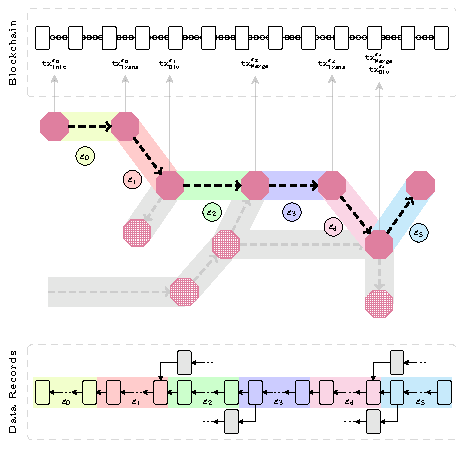
\includegraphics[width=.65\linewidth]{Figures/ZupplyNetwork}
    \caption{The lifecycle of a Product in the Zupply framework}
    \label{fig:enter-label}
\end{figure}

The Zupply framework is designed to ensure the integrity and authenticity of a product's historical data, represented as a \gls{dag}. 

This section describes how the Zupply framework can be employed in its main application i.e., \gls{scm}. Entities in our framework refer to participants in a supply chain — including producers, distributors, and retailers — who upload data records related to products. These entities have three primary objectives in this ecosystem: verifying the authenticity of previously uploaded data records, preserving the integrity of their data records over time, and maintaining their anonymity. Figure \ref{fig:enter-label} illustrates all three components of the Zupply framework in an example supply chain.

The initial entity in the supply chain, referred to as $e_{0}$ (e.g., a supplier of raw materials), creates an \gls{aat}, denoted as $T^{e_{0}}_{j_1}$. To accomplish this, $e_{0}$ executes the $\mathsf{Init}$ function, passing the product quantity ($q_{j_1}$) as an argument. Consequently, a new token, $T^{e_{0}}_{j_1}$, is generated, and its commitment, defined as $\texttt{cm}^{e_{0}}_{j_1} := \mathsf{COMM}_{\rho_{j_1}}(T^{e_{0}}_{j_1})$, is transmitted to the blockchain through a transaction termed $\texttt{tx}^{e_{0}}_\mathsf{Init}$. Then updates its localized version of the \textsf{MHT}, and also updates the root $\texttt{rt}_\tau$ on the smart contract ($\mathcal{C}_Z$). The smart contract verifies the correctness of the new root accordingly (as explained in Section \ref{sec:MerkleTreeStructure}). Following this, entity $e_0$ can begin uploading data records to the DCS by utilizing the $\mathsf{Upload}$ function. This function employs a public parameters, referred to as $\textsc{pp}$, to establish a \gls{zkp}, proving the ownership of an authentication token in \textsf{MHT}. Moreover, each data record is signed using a private key, denoted as \( \text{SKsig}^{e_{0}}_{{j_1}} \). $\text{SKsig}_{i}$ and its corresponding $\text{PKsig}_{i}$ are included in \( T^{e_{0}}_{j_1} \) (see Section \ref{sec:zupply-terms-and-concepts}). This ensures the authenticity and integrity of the data.


% , which its corresponding public key \( \text{PKsig}^{e_{0}}_{{j_1}} \) is included in \( T^{e_{0}}_{j_1} \). This ensures the authenticity and integrity of the data.

In supply chains, a product is transferred among various entities, and each entity needs to transfer the ownership of the products they possess. If the entity $e_{0}$ wants to give a batch of products to the next entity $e_{1}$ and the corresponding \gls{aat} to the batch is $T^{e_{0}}_{j_1}$, the entity executes $\mathsf{Trans}$ algorithm, passing the \gls{aat} as one of its arguments. The algorithm generates a new $\Tilde{T}^{e_{1}}_{j_2}$ for the batch and passes it to $e_{1}$ in a secure off chain channel and submits transaction $\texttt{tx}^{e_{0}}_\mathsf{Trans}$ to the blockchain (the \gls{aat} ownership transfer protocol, i.e., \textsf{OT-Protocol}, is presented in Section \ref{sec:Ownership Transfer}). According to the \textsf{OT-Protocol}, $e_{0}$ cannot use $\Tilde{T}^{e_{1}}_{j_2}$ to upload data records since it does not know the corresponding $\text{SKsig}^{e_{1}}_{j_2}$. The transaction $\texttt{tx}^{e_{0}}_\mathsf{Trans}$ contains a \gls{zkp} of four things: (1) knowing the pre-image of the $\texttt{cm}_{j_1}^{e_{0}}$ which is in the \textsf{MHT} without revealing $\texttt{cm}_{j_1}^{e_{0}}$, (2) the included $\texttt{eol}$ in the transaction is related to  $\texttt{cm}_{j_1}^{e_{0}}$, (3) the proof of knowledge of $\Tilde{T}^{e_{1}}_{j_2}$ related to $\texttt{cm}^{e_{1}}_{j_2} := \mathsf{COMM}_\rho(T^{e_{i_2}}_{j_2})$ included in the transaction (4) the quantity $q_{j_2}=q_{j_1}$ does not change.

In the Zupply framework, entities can split a single authentication token into two using the \textsf{Div} algorithm. For instance, ${e_{1}}$ receives a batch from ${e_{0}}$ and decides to divide it into two smaller batches. One batch is sent to entity ${e_{2}}$, while the other is transferred to a different supply chain. Importantly, both supply chains should be able to access the product's history prior to this division. Additionally, entities have the ability to merge two of their authentication tokens into one using the \textsf{Merge} algorithm. For example, ${e_{2}}$ receives some products from a different supply chain and seeks to batch them together before passing them to ${e_{3}}$. Furthermore, auditors should have the capability to access and review the data records pertaining to both merged supply chains. These functionalities allow for the merging and dividing of data sequences associated with the \gls{aat}s, thereby enabling the maintenance of data in a \gls{dag} structure within the framework.



\subsection{Business Contracts}
\label{App:Business Contracts}


Employing smart contract-enabled blockchain platforms for managing \gls{aat} in the Zupply framework can enable business smart contracts that employ Zupply smart contract $\mathcal{C}_Z$ as a lower layer of their operations. Business smart contracts can provide financial security for entities so they will not rely on a trusted third party for their payments. One example of a business contract is transferring funds upon delivering a product (i.e., transferring an \gls{aat}). Here, we are going to present an example of a business contract $\mathcal{C}_B$ that checks whether a specific \texttt{cm} is uploaded to $\mathcal{C}_Z$ or not. Then, it transfers the funds that were locked in $\mathcal{C}_B$.

In this example, $e_1$ wants to send a product to $e_3$ via $e_2$. $e_2$ uploads data collected from the product till it transfers that to $e_3$. Later on, $e_3$ is going to continue uploading data records related to the product. $e_2$ wants a guaranteed payment by the time the product is delivered to $e_3$. Therefore, any entity who is responsible for the payment ($e_1$ in this example) can lock some funds in $\mathcal{C}_B$. The funds will be transferred to $e_2$ if the entity uploads an \gls{aat} commitment \texttt{cm}, which has been determined at the time of locking the funds to $\mathcal{C}_B$.


The followings are the steps of the the protocol:
\begin{enumerate}
    \item $(\text{PKsig}^{e_3}_1, \text{SKsig}^{e_3}_1) \leftarrow {e_3}^{\mathcal{K}_\mathsf{sig}}(\textsc{pp})$

    \item $e_3$ passes $\text{PKsig}^{e_3}_1$ to $e_1$.

    \item $e_2$: $\rho \xleftarrow{R} \{0, 1\}^O(\lambda)$

    \item $e_2$ passes $\rho$ to $e_1$ upon receiving the product from $e_1$.

    \item $e_1$ creates $\Tilde{T} = (q, \text{PKsig}^{e_3}_{1}, \rho)$ $\texttt{cm} \gets \mathsf{COMM}_\rho(\Tilde{T})$

    \item $e_1$ locks some funds in $\mathcal{C}_B$. These funds will go to $e_2$ whenever \texttt{cm} is uploaded to $\mathcal{C}_Z$ in a $\texttt{tx}_\mathsf{Trans}$ transactions.

    \item Upon receiving the product by $e_3$, both $e_2$ and $e_3$ will engage in the \textsf{OT-Protocol} presented in Section \ref{sec:Ownership Transfer}. $e_3$ will send $\text{PKsig}^{e_3}_1$ to $e_2$ after receiving ``Public key request'' from $e_2$ in the protocol.

    \item $e_2$ uses $\rho$ received from $e_1$ at the time of taking the product and  $\text{PKsig}^{e_3}_1$ received from $e_3$ at the time of giving product. Then outputs a new authentication token commitment \texttt{cm} via \textsf{Trans} algorithm.

    \item In the previous step \texttt{cm} is uploaded to the $\mathcal{C}_Z$ contract; therefore, $e_2$ can take the funds from $\mathcal{C}_B$.
    
\end{enumerate}

\subsection{Data Encryption}
\label{app:Data Encryption}
In the Zupply framework, various key management schemes can be employed to encrypt the private parts of the data records, adapting them according to different applications. In this thesis, we suggest following the Mesh forward secrecy approach for generating keys \cite{altawy2019mesh}. Such that the secret keys $\textsc{k}$ are generated by the radio frequency identification (RFID) tag's Pseudo-random bit generator (PRBG). This approach ensures that, in supply chain applications, a new product owner must have access to all previous encryption keys to trace the product's history effectively. However, it should not be able to decrypt the future data records after the point of transfer to the following entity. Ultimately, the final entity in the supply chain can view the complete history of the associated data progressive chain.


\section{Summary}
\label{app:zupply-summary}


Transferring applications such as \gls{scm}  to permissionless (public) blockchains eliminates the need for trust in a manager and offers a range of benefits, which we will discuss later in this paper. However, by the nature of permissionless blockchain, miners, monitors, auditors and validators see the plain transactions on the blockchain.  This could reveal the privacy of the data providers  and actors in  ownership transfer  of the data from one to another.  However, those will expose inventory information of different business sectors.  So, for blockchain based \gls{scm}, the privacy of data uploader (anonymous problem), and ownership transfer of data (unlinkable problem) is a crucial factor to deploy this technology. 

This chapter proposed a novel anonymous authentication token (\gls{aat}) framework that supports unlinkable \gls{aat} ownership transfer (\gls{aatot}) including unlinkable merging and dividing of \gls{aat}s, realized by \textsf{OT-Protocol} to ensure unlinkability during ownership transfer. The construction leverages zero-knowledge proof (\gls{zkp}) protocols to guarantee anonymity, unlinkability, and authentication. Building on this foundation, we introduce Zupply, a decentralized framework for maintaining directed acyclic graphs (\gls{dag}s) of authentic data records. Designed on a permissionless, smart contract-enabled blockchain, Zupply provides a trustless framework that preserves anonymity and unlinkability among participants while ensuring the integrity and authenticity of data records throughout the supply chain. Its efficiency is realized by minimizing the number of public inputs to the ZKPs, and the \textsf{MHT-Protocol} which updates the root of the MHT on the $\mathcal{C}_Z$  and eliminate the need for storing the entire tree on-chain. 



Zupply adopted a stricter adversary model that previous methods, in which the underlying blockchain platform does not preserve the anonymity of the transaction issuer (adversary's access to $\mathcal{O}^\mathsf{Attr}$). Moreover, transactions scale independently of participant count, Zupply requires no centralized servers or layer-1 changes, and let auditors focus only on relevant records. In contrast, zkLedger \cite{zkLedger2018}has to involve all entities per transaction, Mesh \cite{altawy2019mesh} lacks unlinkability and needs a central server, and DECOUPLES \cite{Maouchi2019DECOUPLES} modifies the base blockchain. 
%======================================================================
\chapter{Zupply Framework Implementation}\label{ch:zupply_implementation}
%======================================================================

\section*{Declaration of Contributions}
This chapter is based on \cite{Badakhshan2024Zupply}. I am the sole author of this chapter.

\section{Introduction}

In the previous two chapters, we introduced the design and security analysis of the Zupply framework. This chapter focuses on its implementation, detailing the 
% construction of \gls{r1cs} instances, the 
instantiation of core building blocks, and the implementation of the zero-knowledge proving and verification algorithms. Specifically, we describe the arithmetic circuits for the \gls{np} problems associated with \textsf{Auth}, \textsf{Trans}, \textsf{Merge}, and \textsf{Div}. These circuits generate \gls{r1cs} instances in a manner that enables succinct zero-knowledge proofs (\gls{zkp}s) while preserving confidentiality. To optimize on-chain costs (i.e., smart contract execution) we minimize the public inputs to these circuits. 
We provide two implementation variants of Zupply based on its \gls{zkp} algorithms. The first employs Groth16 \cite{Groth2016} \gls{zksnark} over BN254 \cite{BNcurve} and BLS12-381 \cite{BLS_curve2003} elliptic curves, accommodating different security levels. The second leverages Aurora \cite{Aurora2019}, a \gls{zksnark} designed for a transparent setup and post-quantum security against quantum-capable malicious provers.

Zupply is implemented in \CC and Solidity, demonstrating both computational and cost efficiency. This development validates the framework's practicality for real-world applications. While directed acyclic graphs (\gls{dag}s) are widely used for maintaining product histories in supply chains, Zupply's utility extends beyond this domain. We show that Zupply provides a practical, cost-efficient, and privacy-preserving solution for decentralized supply chain management (\gls{scm}) systems.

\section{Zupply Arithmetic Circuits}
\label{sec:Zupply Arithmetic Circuits}

\begin{figure*}
    \centering
    \begin{subfigure}[b]{0.35\textwidth}  % Adjusted to fit four images in one row
        \centering
        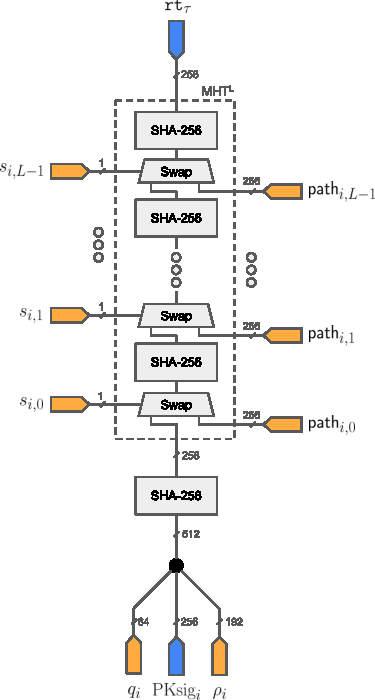
\includegraphics[scale=0.6]{Figures/Auth.pdf} % Replace with your image file
        \caption{\textsf{Auth} circuit}
        \label{fig:Authcircuits}
        
    \end{subfigure}
    \hfill
    \begin{subfigure}[t]{0.60\textwidth}  % Adjusted to fit four images in one row
        \centering
        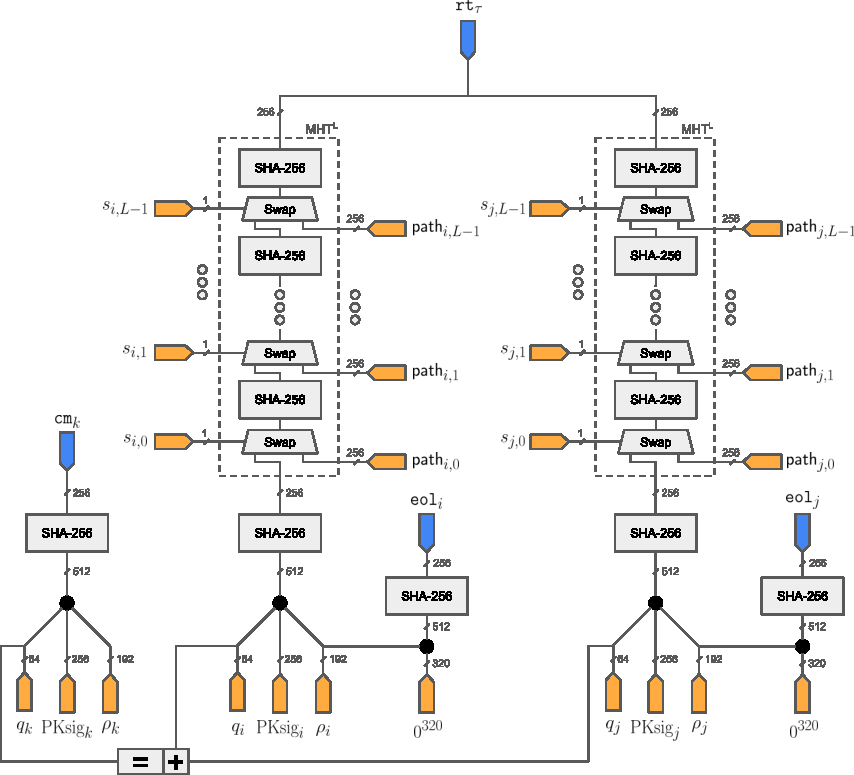
\includegraphics[scale=0.6]{Figures/Merge.pdf} % Replace with your image file
        \caption{\textsf{Merge} circuit}
        \label{fig:Mergecircuits}
    \end{subfigure}
    \hfill\vspace{5mm}
    \begin{subfigure}[t]{0.35\textwidth}  % Adjusted to fit four images in one row
        \centering
        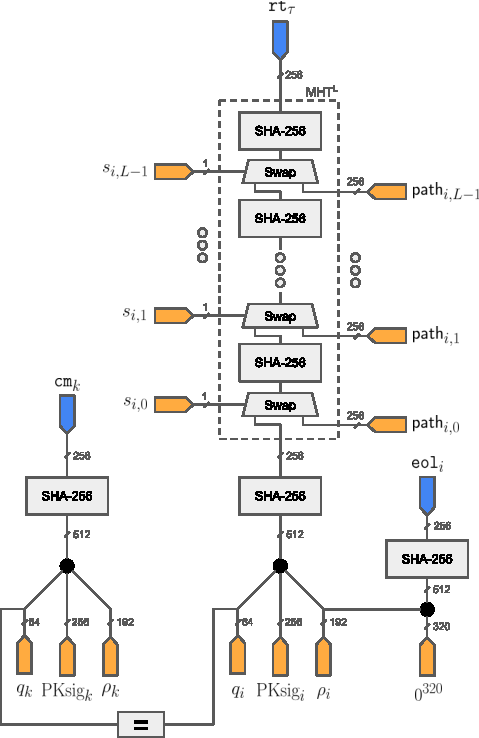
\includegraphics[scale=0.6]{Figures/Trans.pdf} % Replace with your image file
        \caption{\textsf{Trans} circuit}
        \label{fig:Transcircuits}
        
    \end{subfigure}
    \hfill
    \begin{subfigure}[t]{0.60\textwidth}  % Adjusted to fit four images in one row
        \centering
        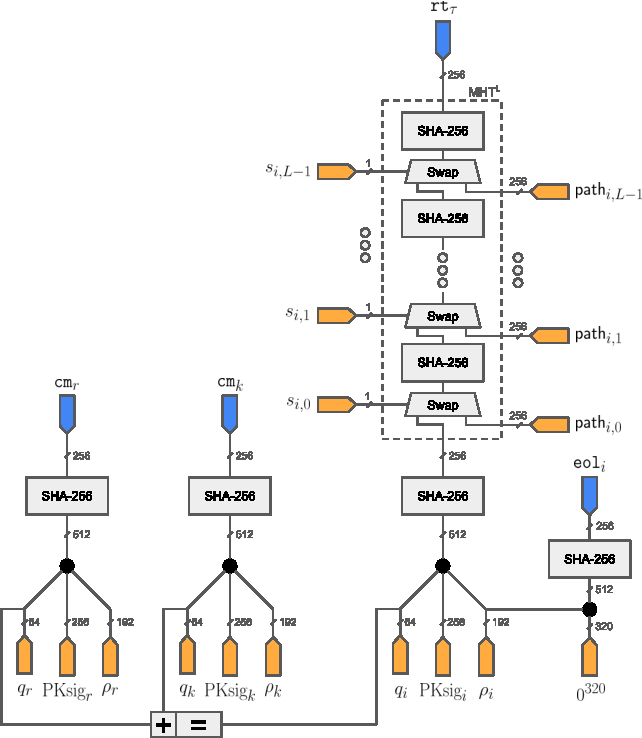
\includegraphics[scale=0.6]{Figures/Div.pdf} % Replace with your image file
        \caption{\textsf{Div} circuit}
        \label{fig:Divcircuits}
        
    \end{subfigure}
    
   \caption[Zupply arithmetic circuits]{Schematic representation of the arithmetic circuits for \gls{zkp}s in the Zupply framework. The Merkle hash tree has a depth of $L$, with public inputs highlighted in \textcolor{blue}{\textbf{blue}}. Inputs highlighted in \textcolor{orange}{\textbf{orange}}, along with the intermediate values within the arithmetic circuits, are private (auxiliary) inputs. The hash function used in the implementation is SHA-256.}
    \label{fig:circuits}
\end{figure*}


The \textsf{Auth}, \textsf{Trans}, \textsf{Merge}, and \textsf{Divide} algorithms in the Zupply framework generate \gls{zkp}s to demonstrate knowledge of the pre-image for one or two commitments to anonymous authentication tokens (\gls{aat}s) in the Merkle hash tree (\textsf{MHT}), with the root at time $\tau$ is denoted by $\texttt{rt}_\tau$. These \gls{zkp}s are used in Zupply algorithms to prove ownership of an \gls{aat} for authenticating a data record or to transfer ownership of the \gls{aat}s. In all cases, the prover avoids revealing the \gls{aat} or its commitment stored in the \textsf{MHT}. Figure \ref{fig:circuits} shows a schematic view of the arithmetic circuits associated with each of these \gls{zkp}s.


These circuits represent the \gls{np} problem related to each \gls{zkp} and are converted into \gls{r1cs}, which are satisfied only when the prover provides consistent inputs to the constraint system. For example, in a circuit designed to prove knowledge of the pre-image of a leaf in a Merkle hash tree with root \texttt{rt}, without revealing the specific leaf, the root of the Merkle hash tree is given as a public input. The private inputs include the corresponding leaf pre-image and the Merkle proof. These private inputs must align with the root and satisfy the circuit constraints. As a result, the prover must provide valid private inputs, thereby demonstrating knowledge of the pre-image of a leaf in the Merkle hash tree.
In the Zupply framework, the root value is determined by the shared \textsf{MHT}, which is maintained within the framework and serves as a public input to the circuits. The prover must demonstrate knowledge of the pre-image of a leaf in the fully decentralized \textsf{MHT}. Importantly, this process does not reveal any information about the \gls{aat} or its commitment (the leaf itself).



Each arithmetic circuit in the Zupply framework includes a proof of knowledge for one or two leaves within the \textsf{MHT}. These circuits are constructed using the arithmetic circuits for the hash function and the Merkle hash tree. The \gls{r1cs}  generated by the hash function arithmetic circuit is satisfied if and only if, for a given input value $x$ assigned to the circuit, the output value $y$ satisfies $y = \mathcal{H}(x)$, where $\mathcal{H}$ is the hash function.
The arithmetic circuit of the Merkle hash tree implements the Merkle proving algorithm. At each level, a hash function output is concatenated to either the left or right of its adjacent hash. The concatenated value is then input to the hash function of the subsequent layer, continuing until the root is reached. Formally, this chain of hash functions is expressed as:
\[
h_{i,j+1} = \mathcal{H}\left( s_{i,j}\cdot(h_{i,j} \,|\ \textsf{path}_{i,j}) + (1-s_{i,j})\cdot(\textsf{path}_{i,j} \,|\ h_{i,j}) \right),
\]
where at layer $j$, $h_{i,j}$ is the output from the previous hash in the chain. Let $h_{i,0}$ denote the $i$-th leaf value and $h_{i,L}$ is equal to the root \texttt{rt}. $\textsf{path}_{i,j}$ represents the adjacent hash at layer $j$ in the Merkle proof related to index $i$, and $s_{i,j} \in \{0,1\}$ determines whether $h_{i,j}$ is concatenated to the left or right of its adjacent hash. 
The arithmetic circuit responsible for managing this order selection is called the ``Swap'' block. The \gls{r1cs}  generated by the arithmetic circuit of a Merkle hash tree with $L$ layers is satisfied if and only if the leaf $h_0$ exists in a Merkle hash tree with root \texttt{rt}, and the Merkle proof, comprising $\{\textsf{path}_{i,0}, \dots, \textsf{path}_{i,L-1}\}$ and $\{s_{i,0}, \dots, s_{i,L-1}\}$, is consistent with both the leaf and the root.


In the following, we delve into the details of each circuit.



\subsection{\textsf{Auth} Circuit} 
The \textsf{Auth} circuit, illustrated in Figure \ref{fig:Authcircuits}, generates the \gls{zkp} $\pi_\textsf{Auth}$, which is embedded in data records to prove that the data creator possesses an \gls{aat} within a Merkle hash tree. The root $\texttt{rt}_\tau$ serves as a public input to this proof to allow the auditor to verify that the commitment to the claimed \gls{aat} is stored in the \textsf{MHT} with root $\texttt{rt}_\tau$. Specifically, the prover asserts, ``she knows a preimage of one of the commitments to an \gls{aat} in the \textsf{MHT} with root $\texttt{rt}_\tau$,'' without revealing which commitment. Additionally, the PKsig associated with the \gls{aat} is also provided as a public input. The data creator signs the data record using the corresponding SKsig, thereby proving that the data has been signed by the token owner and remains unaltered.


\subsection{\textsf{Trans} Circuit} 
The \textsf{Trans} circuit generates the \gls{zkp} $\pi_\textsf{Trans}$, which is submitted to the blockchain platform when an entity transfers ownership of an \gls{aat} during \textsf{OT-Protocol}. Specifically, it obsoletes an \gls{aat} owned by the entity and creates a new \gls{aat} that is consistent with the obsoleted \gls{aat}. The circuit used for generating this proof is depicted in Figure \ref{fig:Transcircuits}.  In the \textsf{Trans} circuit, the pre-images of the commitments to both the new and obsoleted \gls{aat}s are private inputs. The circuit ensures that the $q$ value, representing the quantity of the product, remains unchanged. The commitment to the new \gls{aat} serves as a public input to the circuit, which will be added to the \textsf{MHT}. Additionally, the end of life (\texttt{eol}) value of the obsoleted \gls{aat} is a public input to the circuit and is published on the blockchain platform. This ensures that an entity cannot reuse an \gls{aat} included in the \textsf{MHT} but transferred before. In this proof, the prover asserts: ``She knows an \gls{aat} in the \textsf{MHT} with root $\texttt{rt}_\tau$, where the end-of-life value of the claimed token is \texttt{eol}, and she has created a new \gls{aat} with a commitment \texttt{cm}, such that the quantity in the new token matches the quantity in the originally claimed token.''



\subsection{\textsf{Merge} Circuit} 
The \textsf{Merge} circuit is similar to the \textsf{Trans} circuit, but it merges two existing commitments to two known \gls{aat}s in \textsf{MHT} with root $\texttt{rt}$. Hence, this circuit generates the \gls{zkp} $\pi_\textsf{Merge}$ which proves the knowledge of two \gls{aat}s, where their corresponding \texttt{eol}s are public inputs to this circuit, allowing the verification algorithm to check whether those \gls{aat}s have been transferred before. This circuit also guarantees that the quantity of the product in the new commitment is equivalent to the sum of the product quantities in the two preceding \gls{aat}s. The new commitment to the new \gls{aat} is a public input to this circuit.


\subsection{\textsf{Div} Circuit} 
The \textsf{Div} circuit is the opposite of the \textsf{Merge} circuit. It generates the \gls{zkp} $\pi_\textsf{Div}$, which proves that a known existing \gls{aat} in \textsf{MHT} with root $\texttt{rt}$ divides into two new \gls{aat}s. The \texttt{eol} of the divided token and the commitments to the two new \gls{aat}s are public inputs to this circuit. This circuit ensures consistency in the product quantity before and after division, so that the sum of the $q$ values in the new tokens equals the $q$ value in the original \gls{aat}.


\section{Cryptographic Primitives and Parameters}
In this section, we present the instantiation of each building block  of the Zupply framework, considering a 128-bit security level. 

\subsection{Blockchain platform }
Ethereum provides the highest level of security among all ethereum virtual machine (\gls{evm}) compatible blockchains, such as Arbitrum and Avalanche \cite{Neiheiser2023PracticalLimitations, Kalodner2018Arbitrum, Avalanche}. Therefore, we have selected Ethereum as the blockchain platform upon which Zupply is built. If Zupply remains practical with respect to the costs incurred when calling the smart contract $\mathcal{C}_Z$, then its feasibility extends to other \gls{evm}-compatible blockchains as well. To realize the proof-of-inclusion ($\mathbf{L}_\tau^\mathsf{PI}(\texttt{rt})$), Ethereum employes Merkle Patricia tree (trie) \cite{PatriciaTree, ethereum} and provides $\texttt{eth\_getProof}$ API which is elaborated in EIP-1186 \cite{Jentzsch2018}. 


\subsection{Decentralized Cloud Storage (DCS)}

Zupply utilizes the 
InterPlanetary File System
(\gls{ipfs}) network \cite{Benet2014} for file storage, offering flexibility in data management based on the preferences of the supply chain entities. For instance, entities can opt to share their data records directly from their computers via a Tor hidden service \cite{Loshin2013PracticalAnonymity} to obscure their IP address, or they can entrust storage to major stakeholders within the supply chain. These stakeholders then anonymously publish the data records to the \gls{ipfs} network, ensuring availability. Furthermore, Zupply guarantees the authenticity and integrity of data records, which are independently verified by auditors, thus eliminating reliance on \gls{dcs} for this verification. 
% Moreover, integrity is maintained as any data alteration causes the \textsf{Audit} algorithm to return a 0, effectively detecting tampering. 


%as detailed in Definition \ref{def:informal-Authenticity}, 


% Filecoin \cite{filecoin}, a decentralized storage network based on IPFS \cite{ipfs}, is considered a potential candidate for DCS. 
 
% Therefore, we can employ different kinds of instantiations. 



\subsection{Collision-resistance Hash Function}

The collision resistance hash function $\mathcal{H}$ is a 512-bit input to a 256-bit output mapping; namely, $\mathcal{H}:\{0,1\}^{512} \rightarrow \{0,1\}^{256}$. It can be implemented by either SHA-256 or SHA3-256. For SHA-256, it has 512 bit input and 256 output, so there is no padding bits needed. For SHA3-256, the input size is 1088 bits  and outputs 256 bits. So, in this case, padding is needed. In our implementation, we selected SHA-256 for its simplicity and wide adoption.  

\subsection{Statistically-hiding Commitment}
We instantiate the commitment scheme \textsf{COMM} via $\mathcal{H}$. Such that 
% for computing the commitment to $\Tilde{T} := (q, \text{PKsig}, \rho)$, 
$\texttt{cm}:=\mathsf{COMM}_\rho(\Tilde{T}) = \mathcal{H}(q||\text{PKsig}||[\rho]_{224})$
Where, $q \in \{0, 1\}^{32}$, $\text{PKsig} \in \{0, 1\}^{256}$, and $\rho \in \{0, 1\}^{512}$. Moreover, $[\rho]_{224}$ denotes that the $512$-bit $\rho$ is truncated to $224$ bits by dropping most significant bits. Both $\text{PKsig}$ and $\rho$ 
% (which is the output of a cryptographically strong random number generator (RNG) \cite{NISTPRNG}) 
can serve as randomness for the commitment. 
% Operator $\xleftarrow{R}$ is a cryptographically strong random number generator (RNG) \cite{NISTPRNG}.  The Digital signature algorithm used in the experiment is  the curve Secp256k1 \cite{brown2009standards}.

\subsection{Merkle Hash Tree}
\textsf{MHT} is constructed based on the collision resistance hash function $\mathcal{H}$ (i.e., SHA-256). Let the number of layers $L$ be equal to 20, then \textsf{MHT} has $2^{20} -1$ nodes, and each node has 256 bits. Consequently, the tree requires 32 MB of storage. Recall that the tree is stored off-chain on entities' $\textsc{Z-Node}$ software, and only the root \texttt{rt} is maintained on the smart contract $\mathcal{C}_Z$.


\subsection{Strongly-unforgeable Digital Signature}

The signature scheme algorithm \textsf{Sig} used in the framework is Elliptic Curve Schnorr signatures (EC-Schnorr) \cite{Schnorr1991Signature} over the elliptic curve secp256k1 \cite{sec2_2010} where the size of both PKsig and SKsig are 256 bits and signature has 512 bits. The algorithm uses SHA-256 as the hash function required for the signatures. This algorithm satisfies the \textit{SUF-CMA} security property.

% \subsection{Public-key encryptions}
% Zupply framework employs Elliptic Curve Integrated Encryption Scheme (ECIES) over secp256k1 \cite{sec2_2010} for $\mathsf{Enc}$. This algorithm enables 256-bit PKenc and SKenc keys and satisfies \textit{IND-CCA} security property \cite{katz2020introduction}.

\subsection{Symmetric-key Encryption}
For \textsf{SymEnc}, we use 128-bit advanced encryption standard (AES-128) algorithm in cipher block chaining (CBC) mode which satisfies \textit{IND-CPA} security property \cite{rogaway2011evaluation, sibleyras2020Security}.

\section{zkSNARK Instantiations}
The choice of \gls{zksnark} protocol in the Zupply framework enables a trade-off between computational efficiency and enhanced security properties, such as post-quantum security and a transparent setup.

\subsection{Groth16}

In the first implementation variant of the Zupply framework, we employ Groth16 \cite{Groth2016}, a \gls{zksnark} known for generating succinct proofs and enabling fast verification. This protocol is a pairing-based \gls{zksnark} for \gls{r1cs}. The scheme requires a trusted setup phase that can be done via a secure multi-party computation (\gls{smpc}) \cite{Ben-Sasson2015SecureSampling, Nikolaenko2024PowersofTau}.
We evaluate the implementation using two elliptic curves: BN254 \cite{BNcurve}, offering the fastest algorithms and the smallest proof sizes and approximately 100-bit security \cite{Barbulescu2019}, and BLS12-381 \cite{BLS_curve2003}, designed for 128-bit security.


By using the Groth16 \gls{zksnark} in the Zupply framework, the verification keys ($\text{vk}_\mathbbm{x}$), stored in $\mathcal{C}_Z$, remain small when the number of public inputs ($x_\mathbbm{x}$) is minimal. Additionally, the verification algorithm ($\mathsf{Verify}$) of Groth16 is less complex compared to other \gls{zksnark}s. Due to the high cost of on-chain storage, this efficiency makes Groth16 particularly suitable for public blockchains where execution and storage costs are high.
In Groth16, the proof size remains constant regardless of the number of constraints in the associated \gls{r1cs}. The proof is denoted as \(\pi \in \mathbb{G}_1^2 \times \mathbb{G}_2\), where \(\mathbb{G}_1\) consists of points on the elliptic curve, and \(\mathbb{G}_2\) comprises points on a twist of the curve.  

The size of the verification key \(\textsf{vk}\) depends on the number of public inputs in each \gls{r1cs} instance within the Zupply framework. The public input of the instances in the Zupply framework are denoted as \(x_\mathsf{Auth}\), \(x_\mathsf{Trans}\), \(x_\mathsf{Merge}\), and \(x_\mathsf{Div}\).
Let \(|x_\mathbbm{x}|\) represent the number of public inputs for an instance \(\mathbbm{x}\). As described in \cite{Groth2016}, \(\textsf{vk}\) consists of \(|x_\mathbbm{x}| + 2\) elements in \(\mathbb{G}_1\) and three elements in \(\mathbb{G}_2\). It may also include a precomputed element in \(\mathbb{G}_T\) via the bilinear pairing \( e: \mathbb{G}_1 \times \mathbb{G}_2 \to \mathbb{G}_T \) applied to two specific elements in \(\textsf{vk}\), since the verification process requires only their pairing, not those elements themselves. Consequently, one element from each of \(\mathbb{G}_1\) and \(\mathbb{G}_2\) can be omitted from \(\textsf{vk}\) and replaced by an element in \(\mathbb{G}_T\).

In the Zupply framework, every public input is represented as either a 256-bit hash or a 256-bit public key. However, like other scalar elements in \gls{r1cs} instances, these inputs must belong to the scalar prime field of the underlying elliptic curve. Since the scalar field elements of BN254 and BLS12-381 have bit-lengths of 254 and 255 bits, respectively, each 256-bit value is split into two 128-bit public inputs to minimize the public input size. In contrast, the original implementation of the SHA-256 arithmetic circuit in \cite{libsnark} treats each 256-bit hash as 256 distinct public inputs, significantly increasing the size of the verification keys. Based on our construction, the number of public inputs represented as $n(x_\mathbbm{x})$ in Table \ref{tab:zksize} are double the count of public inputs as per the arithmetic circuits presented in Section \ref{sec:Zupply Arithmetic Circuits}. Moreover, the size of the proving key \textsf{pk} is determined by the number of constraints in each instance and the proving keys in the Zupply framework are stored off-chain on the devices of entities. The number of constraints is determined by the size of the circuit implementing \gls{np} statements in Section \ref{sec:Zero-knowledge Proofs}. 

\subsubsection{Over BN254 Curve}
We initially implement the Groth16 zkSNARK over the BN254 curve. The curve was generally assumed to offer around 128 bits of security \cite{BNcurve}; However, research by Kim et al. \cite{Kim2015Extended} suggests that its actual security level might be lower. In Groth16, the proof size is constant, denoted as \(\pi \in \mathbb{G}_1^2 \times \mathbb{G}_2\), where \(\mathbb{G}_1\) consists of points on the BN254 elliptic curve, and \(\mathbb{G}_2\) comprises points on a twist of the BN254. Consequently, the proof size is 128 bytes, regardless of the size of the number of constraints in the \gls{r1cs} related to the proof.
Since Ethereum only provides pre-compiled contracts for the BN254 curve \cite{EIP197, Housni2022Families}, we selected this pairing-friendly curve for the on-chain Groth16 verification algorithms implementation. 

\subsubsection{Over BLS12-381 Curve}
To strengthen the security of our framework, we replace the BN254 curve with BLS12-381, which offers 128-bit security. However, as of the time of writing, Ethereum does not provide precompiled support for operations over this curve \cite{Vlasov2020}. Consequently, we did not implement our smart contract $C_\mathcal{Z}$ using BLS12-381, leaving this for future work. Adopting this curve increases the proof size to 192 bytes regardless of the size of the number of constraints in  \gls{r1cs}. Table \ref{tab:zksize} compares the verification and proving key sizes for each instance in Zupply using both the BN254 and BLS12-381 curves.

\begin{table}
 \caption[Comparison of the Groth16 key sizes for each NP statement in Zupply]{Comparison of verification and proving key sizes of Groth16 \gls{zksnark} for \gls{np} statements in the Zupply framework for $L=20$. $\nu = n(x_\mathbbm{x})$ is the number of public inputs, $N$ is the number of constraints, $|\mathsf{vk}_\mathbbm{x}|$ is the size of the verification key in Bytes, and  $|\mathsf{pk}_\mathbbm{x}|$ is the size of the proving key in MegaBytes.}
	\centering

\begin{tabular}{ccccccc}
		\toprule
		\multirow{2}{*}{\textbf{$\mathbbm{x}$}} & \multirow{2}{*}{\textbf{$\nu$}} & \multirow{2}{*}{$N$} & \multicolumn{2}{c}{$|\mathsf{vk}_\mathbbm{x}|$ (B)} & \multicolumn{2}{c}{$|\mathsf{pk}_\mathbbm{x}|$ (MB)} \\
		% \cline{4-7}
		 &  &  & {\footnotesize BN254} & {\footnotesize BLS12-381} & {\footnotesize BN254} & {\footnotesize BLS12-381} \\
		\midrule
        Complexity & - & $O(L)$ & \multicolumn{2}{c}{$O(\nu)$}  & \multicolumn{2}{c}{$O(N)$}\\
        
		${\textsf{Auth}}$ & 4  & 588,248  & 768 & 1,152 & 182.5 & 456.3\\
		
		${\textsf{Trans}}$ & 6  & 642,876  & 896 & 1,344 & 200 & 246.75\\
		${\textsf{Merge}}$ & 8 & 1,258,337  & 1,024 & 1,536 & 393.8 & 447.93\\
		${\textsf{Div}}$ & 8 & 670,091  & 1,024 & 1,536 & 210 & 262.5\\
		\bottomrule
	\end{tabular}
	\label{tab:zksize}
\end{table}

\subsection{Aurora}

In the first implementation variant of the Zupply framework, we employ Aurora \cite{Aurora2019}. It is a \gls{zksnark} protocol  that offers transparent-setup, which eliminates the necessity for a trusted parties in the setup phase. Aurora is built upon particularly the Interactive Oracle Proofs (\gls{iop}s) \cite{Ben-Sasson2016IOP} for \gls{r1cs} obtained by the Fast Reed-Solomon Interactive Oracle Proof of Proximity (\gls{fri}) protocol for low degree testing \cite{FRI2018}. Aurora notably avoids dependence on hard mathematical problems such as discrete logarithms or integer factorization, which makes Aurora plausibly post-quantum secure. Aurora relies on minimal assumptions as it requires only a collision-resistant hash function. This makes it a suitable choice for transitioning the Zupply framework toward enhanced post-quantum security.


Since the \gls{r1cs} constraints generated for the Zupply framework in the previous implementation have their elements in the scalar field associated with the chosen elliptic curve, we used the Aurora implementation over the same finite fields and on multiplicative groups. But, Aurora can also be used over binary extension fields and additive groups, which can make its computations faster due to simpler arithmetic operations and reduced computational overhead. We chose the former configuration for compatibility with the first implementation.




\section{Software Implementation}

In this section, we provide a detailed overview of the \CC software implementation\footnote{The implementation is available at \url{https://github.com/mtbadakhshan/zupply-zkp}} for each variant discussed above. Additionally, we introduce a baseline model for comparison, which does not incorporate privacy preservation. 

\subsection{Baseline Model}
To assess the cost overhead introduced by privacy preservation using \gls{zkp}s in the Zupply framework for a supply chain management (\gls{scm}) application, we propose a non-privacy-preserving baseline model that maintains the same functionality; specifically, (non-anonymous) authentication tokens for off-chain data uploading. In the baseline model's smart contract, a token owned by an entity $e_i$ holds $e_i$'s address ($\text{BPAddr}^{e_i}$) and is only transferable by $e_i$. Furthermore, each token holds a quantity, enabling the merging and dividing of tokens. The token owner $e_i$ can use the private key corresponding to $\text{BPAddr}^{e_i}$ to sign off-chain data records, as explained in ERC-4361 \cite{ERC-4361}, or transfer the token.

\subsection{Groth16 Based Implementation}
For the Groth16 \gls{zksnark} instantiation, we employed libsnark \cite{libsnark}, a \CC library developed by SCIPR lab \cite{SCIPR}, which offers implementations of the Groth16 \gls{zksnark} scheme for provers and verifiers. This library was instrumental in generating \gls{r1cs} constraints for \gls{np} problems within our framework, achieved by implementing them as arithmetic circuits. Additionally, to integrate the Groth16 verification algorithm into $\mathcal{C}_Z$, we utilized the ZoKrates \cite{ZoKrates} toolbox. As previously discussed, we only provide the Zupply smart contract implementation using Groth16 over BN254. 

Table \ref{tab:transaction_gas} presents the costs associated with executing transactions in both the Zupply framework and the baseline model on the Ethereum blockchain. 
At the time of deploying $\mathcal{C}_Z$, some one-time costs should be paid as it uploads the code, a 256-bit \texttt{rt}, and all verification keys except $\mathsf{vk}_\mathsf{Auth}$ to blockchain. $\mathsf{vk}$ sizes are listed in Table \ref{tab:zksize}.  Transactions $\texttt{tx}_\mathsf{Trans}$, $\texttt{tx}_\mathsf{Merge}$, and $\texttt{tx}_\mathsf{Div}$ execute \textsf{VerifyTX} on  $\mathcal{C}_Z$ and contain a 256 bytes $\pi$, one or two $20 \times 256$ bits $\mathsf{path}$ (for $L=20$), new $256$-bit \texttt{rt}s,  $256$-bit \texttt{cm}s, and $256$-bit \texttt{eol}s. 
While the deployment cost is a one-time expense, entities incur transaction fees each time they transfer products to the next entity. 

We also implemented the zero-knowledge proving and verification algorithms of the Zupply framework using Groth16 over the BLS12-381 curve. Consequently, the elements in the R1CS constraint system are in the scalar prime field associated with the BLS12-381 curve.

\subsection{Aurora Based Implementation}
\label{sec:aurora-based-Implementation}
The implementation of the Aurora zkSNARK is provided in libiop \cite{libiop}, which utilizes the libff \cite{libff} library for finite field arithmetic. Similarly, libsnark employs an older version of libff for operations involving both finite fields and elliptic curves. To enable the simultaneous execution of prover and verifier algorithms in both zkSNARKs (i.e., Aurora and Groth16) for the \gls{r1cs} constraint systems generated by the arithmetic circuits, we updated several lines of code in the libsnark library to ensure compatibility with the newer version of the libff library\footnote{The new version of the libsnark library is available at: \url{https://github.com/mtbadakhshan/libsnark}}.

The current implementation of the Aurora \gls{zksnark} in libiop \cite{libiop} requires that the number of constraints in the \gls{r1cs} be a power of two, and that the number of variables and public inputs be one less than a power of two. To meet these requirements, constraints and variables are padded with zeros as necessary. Since the prover time, proof size, and verifier time in the Aurora zkSNARK asymptotically depend on the number of constraints, the computational complexity and proof size for any arithmetic circuit encoded into R1CS effectively correspond to those of an R1CS with a number of constraints equal to the next power of two. 


\begin{table}[t] % Gas price 32 Gwei
	\caption[The Cost of Transactions in the Zupply Framework]{Comparison of the transaction costs for the baseline model and the $\mathcal{C}_Z$ smart contract based on Groth16 over BN254 curve and $L=20$. The costs are in Gas and USD, based on ETH's value of USD 2,030.01 and gas price of 32 Gwei at the time of writing.}
	\centering
{
	\begin{tabular}{ccccc}
		\toprule
        & \multicolumn{2}{c}{Zupply} & \multicolumn{2}{c}{Baseline model}\\ %\cline{2-5}
		{Transaction} & {Gas} & {USD} & {Gas} & {USD}\\
		\midrule
		Deployment & 3,088,611 & \$200.63 & 902,355 & \$58.62 \\ % 3058031 * 1.01 = 3088611.31
        % \hline
		$\texttt{tx}_{\textsf{Init}}$ & 133,415 & \$8.67 & 96,166 & \$6.25 \\ %132095 * 1.01 = 
		% \hline
		$\texttt{tx}_{\textsf{Trans}}$ & 448,013 & \$29.10 & 29,649 & \$1.93\\ % 443578 * 1.01 = 
		% \hline
		$\texttt{tx}_{\textsf{Merge}}$ & 455,534 & \$29.59 & 92,382 & \$6.00 \\ %451024 * 1.01 =  455534
		% \hline
		$\texttt{tx}_{\textsf{Div}}$ & 518,701 & \$33.69 & 168,740 & \$10.96\\ % 513566 *1.01
		\bottomrule
	\end{tabular}
 }
	\label{tab:transaction_gas}
\end{table}


\section{Benchmark}
\label{sec:zupply-benchmark}
The benchmarks were conducted on a system featuring an Intel\textsuperscript{\textregistered} Core\texttrademark{} i7-4790 CPU at 3.60~GHz, using 4 physical cores and 8 threads. The system was equipped with 32~GB of DDR3–1333 RAM and ran Ubuntu 20.04 LTS. The CPU governor was set to \textit{Performance} to ensure the CPU operated at its maximum clock speed throughout testing, thus minimizing fluctuations caused by power-saving mechanisms. We used the Google Benchmark library~\cite{google_benchmark} to measure the average execution time for each \textsf{MHT} depth \( L \) and prover and verifier algorithms for each circuit.

\begin{figure}
    \centering
    \scalebox{.81}{
    % \documentclass{standalone}
% \usepackage{pgfplots}
% \pgfplotsset{compat=1.18} % Adjust based on your pgfplots version
% \usepgfplotslibrary{groupplots} % Load the groupplots library for groupplot functionality
% \usepackage{siunitx}
% \pgfplotmarksize=1.5pt
% \begin{document}

% % \begin{figure}
% \centering
\begin{tikzpicture}
\begin{groupplot}[
    group style={
        group size=2 by 1,
        horizontal sep=1cm,
        vertical sep=2cm,
    },
    width=10cm,
    height=6cm,
    xlabel=L,
    % ymode=log,
    grid=both,
    major grid style={black!50},  % Style for major grid lines
    minor grid style={gray!20},   % Style for minor grid lines
    minor tick num=1,             % Number of minor ticks between major ticks
    % ymin=5e4, ymax=.6e9,
    % mark size=1pt,
    % ylabel near ticks,
    % xtick={10,12,14,16,18,20,22,24},
    yticklabel style={/pgf/number format/fixed}%,
    % legend style={at={(0.25,0.98)}, anchor=north}
]

%====================

\nextgroupplot[ylabel=Number of Constraints, title=Aurora, legend to name=zelda3]
\addplot table [x=Range, y={bytes}, col sep=comma] {CSVs/csv_files_BN254/LIBIOP-num_constraints_Merge.csv};
\addlegendentry{\textsf{Merge} Circuit};
\addplot table [x=Range, y={bytes}, col sep=comma] {CSVs/csv_files_BN254/LIBIOP-num_constraints_Div.csv};
\addlegendentry{\textsf{Div} Circuit};
\addplot table [x=Range, y={bytes}, col sep=comma] {CSVs/csv_files_BN254/LIBIOP-num_constraints_Trans.csv};
\addlegendentry{\textsf{Trans} Circuit};
\addplot table [x=Range, y={bytes}, col sep=comma] {CSVs/csv_files_BN254/LIBIOP-num_constraints_Auth.csv};
\addlegendentry{\textsf{Auth} Circuit};
% \coordinate (bot3) at (rel axis cs:1.1,-.55);

%====================
\nextgroupplot[ title=Groth16]
\addplot table [x=Range, y={bytes}, col sep=comma] {CSVs/csv_files_BN254/LIBSNARK-num_constraints_Merge.csv};
\addplot table [x=Range, y={bytes}, col sep=comma] {CSVs/csv_files_BN254/LIBSNARK-num_constraints_Div.csv};
\addplot table [x=Range, y={bytes}, col sep=comma] {CSVs/csv_files_BN254/LIBSNARK-num_constraints_Trans.csv};
\addplot table [x=Range, y={bytes}, col sep=comma] {CSVs/csv_files_BN254/LIBSNARK-num_constraints_Auth.csv};
\coordinate (bot3) at (rel axis cs:-.05,-.5);




% \coordinate (bot2) at (rel axis cs:.5,-.55);
\end{groupplot}
\node at(bot3){\pgfplotslegendfromname{zelda3}};
\end{tikzpicture}
% \end{figure}

% \end{document}
    }
    \caption[Number of constraints in the R1CS instances in Zupply]{The number of constraints in the \gls{r1cs} instances generated by arithmetic circuits in the Zupply framework for both Aurora \cite{Aurora2019} and Groth16 \cite{Groth2016} zkSNARKs, as the Merkle hash tree depth \(L\) varies from 10 to 25.}
    \label{fig:num_constraints}
\end{figure}

We executed the prover and verifier algorithms in Aurora and Groth16 for each circuit in the Zupply framework, using varying numbers of layers in the \textsf{MHT}. Figure \ref{fig:num_constraints} shows the number of constraints generated for each circuit. As previously noted, the Aurora \gls{zksnark} implementation in libiop \cite{libiop} requires the number of constraints to be padded to the next power of two. Consequently, as shown in the figure, the number of constraints for each $L$ in each circuit is increased to the next power of two. This padding introduces significant computational overhead for the prover and verifier algorithms and leads to an increase in proof size.


For each $L$ in each circuit, the computation times of the prover algorithms were averaged over multiple executions using different sets of inputs (i.e., public inputs and auxiliary inputs) to generate proofs. These inputs were randomly generated through  separate functions simulating the circuit, ensuring consistency with the \gls{r1cs} of each circuit. Similarly, the computation times of the verifier algorithms were averaged over executions using different valid proofs generated by the prover algorithm given the aforementioned randomly generated inputs. 
The experiments for the prover and verifier algorithms in Groth16 were conducted using both BN254 and BLS12-381 curves to evaluate the computational overhead introduced by the BLS12-381 curve, which achieves 128 bits of security at the cost of increased execution time for the algorithms. Likewise, the experiments for the prover and verifier algorithms in Aurora were executed over the scalar prime fields associated with the BN254 and BLS12-381 curves, with sizes of 254 and 255 bits, respectively. Figure~\ref{fig:execution_time} shows the execution times of the prover and verifier algorithms for both Groth16 and Aurora \gls{zksnark}s.

\begin{figure}
    \centering
    \scalebox{0.81}{
    % \documentclass{standalone}
% \usepackage{pgfplots}
% \pgfplotsset{compat=1.18} % Adjust based on your pgfplots version
% \usepgfplotslibrary{groupplots} % Load the groupplots library for groupplot functionality
% \usepackage{siunitx}
% \pgfplotmarksize=1.5pt
% \begin{document}

% % \begin{figure}
% \centering
\begin{tikzpicture}
\begin{groupplot}[
    group style={
        group size=2 by 2,
        horizontal sep=1.2cm,
        vertical sep=2cm,
    },
    width=10cm,
    height=7cm,
    xlabel=L,
    ylabel shift=-12pt,
    ymode=log,
    grid=both,
    major grid style={black!50},  % Style for major grid lines
    minor grid style={gray!20},   % Style for minor grid lines
    minor tick num=1,             % Number of minor ticks between major ticks
    % ymin=5e4, ymax=.6e9,
    % mark size=1pt,
    % ylabel near ticks,
    % xtick={10,12,14,16,18,20,22,24},
    yticklabel style={/pgf/number format/fixed}%,
    % legend style={at={(0.25,0.98)}, anchor=north}
]

%====================
\nextgroupplot[title=\textsf{Auth}, ylabel=Time (\si{\second}),  legend to name=zelda, legend style={
        legend columns=2, column sep=0.25cm}]

\addplot[mark=oplus, color=blue] table [x=Range, y={Mean CPU Time (microseconds)}, col sep=comma] {CSVs/csv_files_BLS12-381/BM_PROVER_LIBIOP_Auth.csv};
\addlegendentry{Aurora Prover (255-bit)};
\addplot[mark=square, color=red] table [x=Range, y={Mean CPU Time (microseconds)}, col sep=comma] {CSVs/csv_files_BN254/BM_PROVER_LIBIOP_Auth.csv};
\addlegendentry{Aurora Prover (254-bit)};

\addplot table [x=Range, y={Mean CPU Time (microseconds)}, col sep=comma] {CSVs/csv_files_BLS12-381/BM_VERIFIER_LIBIOP_Auth.csv};
\addlegendentry{Aurora Verifier (255-bit)};
\addplot table [x=Range, y={Mean CPU Time (microseconds)}, col sep=comma] {CSVs/csv_files_BN254/BM_VERIFIER_LIBIOP_Auth.csv};
\addlegendentry{Aurora Verifier (254-bit)};


\addplot table [x=Range, y={Mean CPU Time (microseconds)}, col sep=comma] {CSVs/csv_files_BLS12-381/BM_PROVER_LIBSNARK_Auth.csv};
\addlegendentry{Groth16 Prover (BLS12-381)};
\addplot[mark=diamond*, color=red] table [x=Range, y={Mean CPU Time (microseconds)}, col sep=comma] {CSVs/csv_files_BN254/BM_PROVER_LIBSNARK_Auth.csv};
\addlegendentry{Groth16 Prover (BN254)};

\addplot table [x=Range, y={Mean CPU Time (microseconds)}, col sep=comma] {CSVs/csv_files_BLS12-381/BM_VERIFIER_LIBSNARK_Auth.csv};
\addlegendentry{Groth16 Verifier (BLS12-381)};
\addplot table [x=Range, y={Mean CPU Time (microseconds)}, col sep=comma] {CSVs/csv_files_BN254/BM_VERIFIER_LIBSNARK_Auth.csv};
\addlegendentry{Groth16 Verifier (BN254)};


%====================
\nextgroupplot[ title=\textsf{Trans}]
\addplot[mark=oplus, color=blue] table [x=Range, y={Mean CPU Time (microseconds)}, col sep=comma] {CSVs/csv_files_BLS12-381/BM_PROVER_LIBIOP_Trans.csv};
\addplot[mark=square, color=red]  table [x=Range, y={Mean CPU Time (microseconds)}, col sep=comma] {CSVs/csv_files_BN254/BM_PROVER_LIBIOP_Trans.csv};

\addplot table [x=Range, y={Mean CPU Time (microseconds)}, col sep=comma] {CSVs/csv_files_BLS12-381/BM_VERIFIER_LIBIOP_Trans.csv};
\addplot table [x=Range, y={Mean CPU Time (microseconds)}, col sep=comma] {CSVs/csv_files_BN254/BM_VERIFIER_LIBIOP_Trans.csv};

\addplot table [x=Range, y={Mean CPU Time (microseconds)}, col sep=comma] {CSVs/csv_files_BLS12-381/BM_PROVER_LIBSNARK_Trans.csv};
\addplot[mark=diamond*, color=red] table [x=Range, y={Mean CPU Time (microseconds)}, col sep=comma] {CSVs/csv_files_BN254/BM_PROVER_LIBSNARK_Trans.csv};


\addplot table [x=Range, y={Mean CPU Time (microseconds)}, col sep=comma] {CSVs/csv_files_BLS12-381/BM_VERIFIER_LIBSNARK_Trans.csv};
\addplot table [x=Range, y={Mean CPU Time (microseconds)}, col sep=comma] {CSVs/csv_files_BN254/BM_VERIFIER_LIBSNARK_Trans.csv};

%====================
\nextgroupplot[ylabel=Time (\si{\second}), title=\textsf{Merge}]
\addplot[mark=oplus, color=blue] table [x=Range, y={Mean CPU Time (microseconds)}, col sep=comma] {CSVs/csv_files_BLS12-381/BM_PROVER_LIBIOP_Merge.csv};
\addplot[mark=square, color=red]  table [x=Range, y={Mean CPU Time (microseconds)}, col sep=comma] {CSVs/csv_files_BN254/BM_PROVER_LIBIOP_Merge.csv};

\addplot table [x=Range, y={Mean CPU Time (microseconds)}, col sep=comma] {CSVs/csv_files_BLS12-381/BM_VERIFIER_LIBIOP_Merge.csv};
\addplot table [x=Range, y={Mean CPU Time (microseconds)}, col sep=comma] {CSVs/csv_files_BN254/BM_VERIFIER_LIBIOP_Merge.csv};

\addplot table [x=Range, y={Mean CPU Time (microseconds)}, col sep=comma] {CSVs/csv_files_BLS12-381/BM_PROVER_LIBSNARK_Merge.csv};
\addplot[mark=diamond*, color=red] table [x=Range, y={Mean CPU Time (microseconds)}, col sep=comma] {CSVs/csv_files_BN254/BM_PROVER_LIBSNARK_Merge.csv};

\addplot table [x=Range, y={Mean CPU Time (microseconds)}, col sep=comma] {CSVs/csv_files_BLS12-381/BM_VERIFIER_LIBSNARK_Merge.csv};
\addplot table [x=Range, y={Mean CPU Time (microseconds)}, col sep=comma] {CSVs/csv_files_BN254/BM_VERIFIER_LIBSNARK_Merge.csv};

%====================
\nextgroupplot[ title=\textsf{Div}]
\addplot[mark=oplus, color=blue] table [x=Range, y={Mean CPU Time (microseconds)}, col sep=comma] {CSVs/csv_files_BLS12-381/BM_PROVER_LIBIOP_Div.csv};
\addplot[mark=square, color=red]  table [x=Range, y={Mean CPU Time (microseconds)}, col sep=comma] {CSVs/csv_files_BN254/BM_PROVER_LIBIOP_Div.csv};

\addplot table [x=Range, y={Mean CPU Time (microseconds)}, col sep=comma] {CSVs/csv_files_BLS12-381/BM_VERIFIER_LIBIOP_Div.csv};
\addplot table [x=Range, y={Mean CPU Time (microseconds)}, col sep=comma] {CSVs/csv_files_BN254/BM_VERIFIER_LIBIOP_Div.csv};

\addplot table [x=Range, y={Mean CPU Time (microseconds)}, col sep=comma] {CSVs/csv_files_BLS12-381/BM_PROVER_LIBSNARK_Div.csv};
\addplot[mark=diamond*, color=red] table [x=Range, y={Mean CPU Time (microseconds)}, col sep=comma] {CSVs/csv_files_BN254/BM_PROVER_LIBSNARK_Div.csv};

\addplot table [x=Range, y={Mean CPU Time (microseconds)}, col sep=comma] {CSVs/csv_files_BLS12-381/BM_VERIFIER_LIBSNARK_Div.csv};
\addplot table [x=Range, y={Mean CPU Time (microseconds)}, col sep=comma] {CSVs/csv_files_BN254/BM_VERIFIER_LIBSNARK_Div.csv};
\coordinate (bot1) at (rel axis cs:-0.07,-.55);

%***********************************
%***********************************
% \nextgroupplot[cycle list shift=8, ymode=normal, ylabel=Size (Bytes), title=$\pi_\textsf{Auth}$, legend to name=zelda2]

% \addplot table [x=Range, y={bytes}, col sep=comma] {CSVs/csv_files_BN254/LIBIOP-Proof_size_Auth.csv};
% \addlegendentry{Aurora Proof Size};
% \addplot table [x=Range, y={bytes}, col sep=comma] {CSVs/csv_files_BN254/LIBSNARK-Proof_size_Auth.csv};
% \addlegendentry{Groth16 Proof Size };
% \coordinate (bot2) at (rel axis cs:.5,-.55);

\end{groupplot}

\node at(bot1){\pgfplotslegendfromname{zelda}};
% \node at(bot2){\pgfplotslegendfromname{zelda2}};
\end{tikzpicture}
% \end{figure}

% \end{document}
    }
    \caption[The runtime of the prover and verifier algorithms in Zupply]{Prover and Verifier for Groth16 and Aurora in Zupply. Groth16 is evaluated on BN254 and BLS12-381, while Aurora uses their 254-bit and 255-bit scalar fields. $L$ denotes \textsf{MHT} layers.}

    \label{fig:execution_time}
\end{figure}

\begin{figure}
    \centering
    \scalebox{0.81}{
    % \documentclass{standalone}
% \usepackage{pgfplots}
% \pgfplotsset{compat=1.18} % Adjust based on your pgfplots version
% \usepgfplotslibrary{groupplots} % Load the groupplots library for groupplot functionality
% \usepackage{siunitx}
% \pgfplotmarksize=1.5pt
% \begin{document}

% % \begin{figure}
% \centering
\begin{tikzpicture}
\begin{groupplot}[
    group style={
        group size=1 by 1,
        horizontal sep=1cm,
        vertical sep=2cm,
    },
    width=10cm,
    height=6cm,
    xlabel=L,
    % ymode=log,
    grid=both,
    major grid style={black!50},  % Style for major grid lines
    minor grid style={gray!20},   % Style for minor grid lines
    minor tick num=1,             % Number of minor ticks between major ticks
    % ymin=5e4, ymax=.6e9,
    % mark size=1pt,
    % ylabel near ticks,
    % xtick={10,12,14,16,18,20,22,24},
    yticklabel style={/pgf/number format/fixed}%,
    % legend style={at={(0.25,0.98)}, anchor=north}
]

%====================

\nextgroupplot[ylabel=Proof Size (Kilobytes), title=Aurora, legend to name=zelda3]
\addplot table [x=Range, y  expr=\thisrow{bytes}/1024, col sep=comma] {CSVs/csv_files_BN254/LIBIOP-Proof_size_Merge.csv};
\addlegendentry{$\pi_\textsf{Merge}$};
\addplot table [x=Range, y expr=\thisrow{bytes}/1024, col sep=comma] {CSVs/csv_files_BN254/LIBIOP-Proof_size_Div.csv};
\addlegendentry{$\pi_\textsf{Div}$};
\addplot table [x=Range, y expr=\thisrow{bytes}/1024, col sep=comma] {CSVs/csv_files_BN254/LIBIOP-Proof_size_Trans.csv};
\addlegendentry{$\pi_\textsf{Trans}$};
\addplot table [x=Range, y expr=\thisrow{bytes}/1024, col sep=comma] {CSVs/csv_files_BN254/LIBIOP-Proof_size_Auth.csv};
\addlegendentry{$\pi_\textsf{Auth}$};
% \coordinate (bot3) at (rel axis cs:1.1,-.55);

%====================
% \nextgroupplot[ title=Aurora (BLS12-381)]
% \addplot table [x=Range, y={bytes}, col sep=comma] {CSVs/csv_files_BLS12-381/LIBIOP-Proof_size_Merge.csv};
% \addplot table [x=Range, y={bytes}, col sep=comma] {CSVs/csv_files_BLS12-381/LIBIOP-Proof_size_Div.csv};
% \addplot table [x=Range, y={bytes}, col sep=comma] {CSVs/csv_files_BLS12-381/LIBIOP-Proof_size_Trans.csv};
% \addplot table [x=Range, y={bytes}, col sep=comma] {CSVs/csv_files_BLS12-381/LIBIOP-Proof_size_Auth.csv};
\coordinate (bot3) at (rel axis cs:1.21,0.5);




% \coordinate (bot2) at (rel axis cs:.5,-.55);
\end{groupplot}
\node at(bot3){\pgfplotslegendfromname{zelda3}};
\end{tikzpicture}
% \end{figure}

% \end{document}
    }
    \caption[The proof sizes in Zupply based on Aurora]{Proof sizes of Aurora. The proof sizes for 255-bit and 254-bit prime fields are identical, as both require 4×64-bit limbs on a 64-bit architecture. $L$ denotes \textsf{MHT} layers.  Groth16 proof sizes are 128 bytes (BN254) and 192 bytes (BLS12-381). }
    \label{fig:proof_size}
\end{figure}


Figure~\ref{fig:proof_size} illustrates the proof sizes for Aurora. The results are provided for each circuit in the Zupply framework, with the number of \textsf{MHT} layers ranging from $10$ to $25$. Note that the proof size for Groth16 is independent of the circuit; it is 128 bytes for the BN254 curve and 192 bytes for the BLS12-381 curve. As discussed in Section~\ref{sec:aurora-based-Implementation}, the Aurora implementation in Libiop \cite{libiop} increases the prover and verifier computation times and proof sizes to match those of a circuit where the number of constraints, public inputs, and variables are equal to the smallest power of two that exceeds the actual values in the circuit. 

\section{Performance Analysis}


Figure ~\ref{fig:execution_time} demonstrates that operating over BLS12-381 significantly increases the execution times of Groth16 algorithms. This disparity arises because Groth16 algorithms rely heavily on bilinear pairings over elliptic curves. Pairing operations on the BLS12-381 curve are more computationally intensive than those on BN254, primarily due to BLS12-381's larger base field size of 381 bits compared to BN254's 254 bits. However, the scalar field sizes of the two curves are nearly identical, with BN254 and BLS12-381 having scalar fields of  254 and 255 bits, respectively. 

The results clearly show that adopting Aurora into the Zupply framework adds a significant overhead to the runtime of the algorithms. This illustrates the importance of both theoretical and implementation optimizations for current post-quantum transparent setup \gls{zksnark}s and the arithmetic circuits of Zupply. Aurora and many other post-quantum transparent setup \gls{zksnark}s, such as STARK \cite{Ben-Sasson2018STARK} and Fractal \cite{Chiesa2020Fractal}, heavily rely on the fast Fourier transform (\gls{fft}). Although there has been a great deal of research aimed at optimizing these algorithms, using special basis elements (e.g., the Cantor special basis) to construct evaluation domains in these \gls{zksnark}s can still significantly reduce the runtime of additive \gls{fft} algorithms. On the other hand, the arithmetic circuits can be optimized by replacing the standard cryptographic hash function we used (i.e., SHA-256) with algebraic hash functions such as Poseidon \cite{Grassi2021Poseidon}, which require fewer \gls{r1cs} constraints.

Entities handling product histories must store all proving keys ($\mathsf{pk}_\mathbbm{x}$, see Table \ref{tab:zksize}) and a \textsf{MHT} of 32 MB for $L=20$. This requires significant storage due to numerous constraints, but it is manageable even on smartphones. In contrast, auditors, like final customers, only need to store $\mathsf{vk}_\mathsf{Auth}$ (less than 1 KB) and audit only the relevant records.

\section{Evaluation}
Zupply employs off-chain data storage while anonymously authenticating the data, which is a significant advantage considering the high costs associated with on-chain storage\footnote{For example, storing a 1 MB data record on the Ethereum blockchain currently costs over USD 38,000 based on ETH’s value at the time of writing.}. None of the studied related works could provide anonymous authenticated off-chain storage. On-chain storage forces all full nodes in the blockchain platform to maintain a replication of each data record, which is why it is very expensive.

Moreover, the separation of storage and blockchain enhances anonymity, even when an adversary's access to $\mathcal{O}^\mathsf{Attr}$, is assumed. In other words, Zupply employs a more restrictive adversary model in which the underlying blockchain platform (e.g., Ethereum) does not preserve the anonymity of the transaction issuer. Then, if a data record is uploaded to the blockchain platform, the identity of the data uploader will be linked to the data record. However, this adversary's assumption is not considered in any of the previous works. For example, Mesh \cite{altawy2019mesh} and zkLedger \cite{zkLedger2018}, which are deployed over public blockchains, are prone to this attack.


To achive unlinkability among entities involved in a token transfer, we proposed an anonymous authentication token ownership transfer algorithm (\gls{aatot}), presented in Section \ref{sec:Ownership Transfer}. zkLedger requires involving the entire set of entities (including non-participating ones) in each transactions, which has a negative impact on its scalability. zkLedger commits to a value of zero for non-participating entities to obscure the link between the entities involved in the transaction. This increases the size of transactions in zkLedger by increasing the number of participants.  In contrast, the size of transactions in Zupply is independent of the number of entities. Mesh requires the first entity in a supply chain to send a list of the accounts of the involved entities in the supply chain to a smart contract, while the list is sorted by the order in which the products are going to be owned. Therefore, it cannot  provide unlinkability. Moreover, since adding a new entity to the supply chain list in the Mesh framework requires a new setup, Mesh cannot provide a good scalability.

DECOUPLES \cite{Maouchi2019DECOUPLES} proposes a layer-1 blockchain where  multilayered linkable spontaneous anonymous group (\gls{mslag}) ring signatures and stealth addresses are used to provide full anonymity and unlinkability.  However, DECOUPLES is not fully decentralized (trustless) because it requires the mass adoption of the protocol among a large number of miners. However, Zupply does not require any changes to the layer-1 blockchain platform and is fully applicable to existing public blockchains. This enables it to facilitate the complete decentralization of current public blockchains. Additionally, although Mesh also operates over decentralized public blockchains, it requires a centralized Mesh server, which makes the protocol not fully trustless.


\begin{table}
	\caption[Comparison of Security Properties and Cost Efficiency in Privacy-Preserving Supply Chain Management Schemes]{Comparison of security properties and costs among Zupply, related works, and baseline model.
		\fullcirclegreen, \halfcirclegreen, and \emptycirclegreen \ indicate that the framework satisfies, partially satisfies, and does not satisfy a security property, respectively. \fulldiamondred, \halfdiamondred, and \emptydiamondred \ indicate that the framework has high, medium, and low cost, respectively.
	}
	\centering
	\begin{tabular}{|c|c|c|c|c|c|c|c|c|c|c|c|}
		\hline
		& \multicolumn{6}{c|}{Security Properties} & \multicolumn{5}{c|}{Costs} \\ \cline{2-12} 
		& \multirow{2}{0.4cm}{\rotatebox[origin=c]{90}{\makebox[3.5cm][l]{Anonymity}}} 
		& \multirow{2}{0.4cm}{\rotatebox[origin=c]{90}{\makebox[3.5cm][l]{$\text{AATOT}^*$}}} 
		& \multirow{2}{0.4cm}{\rotatebox[origin=c]{90}{\makebox[3.5cm][l]{Unlinkability}}} 
		& \multirow{2}{0.4cm}{\rotatebox[origin=c]{90}{\makebox[3.5cm][l]{Integrity}}} 
		& \multirow{2}{0.4cm}{\rotatebox[origin=c]{90}{\makebox[3.5cm][l]{Decentralization}}} 
		& \multirow{2}{0.4cm}{\rotatebox[origin=c]{90}{\makebox[3.5cm][l]{{No Central Server}}}} 
		& \multicolumn{2}{c|}{{Storage}} 
		& \multirow{2}{0.4cm}{\rotatebox[origin=c]{90}{\makebox[3.5cm][l]{{Transfer (on-chain)}}}} 
		& \multirow{2}{0.4cm}{\rotatebox[origin=c]{90}{\makebox[3.5cm][l]
				{{Audit (off-chain)}}}} 
		& \multirow{2}{0.4cm}{\rotatebox[origin=c]{90}{\makebox[3.5cm][l]{Scalability}}} \\ \cline{8-9}
		\multirow{-2}{*}{\makecell[bc]{Framework}}& & & & & & & 
		\makebox[0.4cm][l]{\rotatebox[origin=c]{90}{\makebox[3.2cm][l]{ On-chain}}} 
		& \makebox[0.4cm][l]{\rotatebox[origin=c]{90}{\makebox[3.2cm][l]{ Entity Software}}} & & & \\ \hline \hline
		\textbf{Mesh} \cite{altawy2019mesh}                    & \halfcirclegreen & \makebox[0pt][c]{\scalebox{0.7}[1]{N/A}} & \emptycirclegreen & \fullcirclegreen & \halfcirclegreen & \emptycirclegreen & \fulldiamondred & \emptydiamondred & \makebox[0pt][c]{\scalebox{0.7}[1]{N/A}} & \makebox[0pt][c]{\scalebox{0.7}[1]{N/A}} & \fulldiamondred \\ \hline
		\textbf{DECOUPLES} \cite{Maouchi2019DECOUPLES}            & \fullcirclegreen & \makebox[0pt][c]{\scalebox{0.7}[1]{N/A}} & \fullcirclegreen & \fullcirclegreen & \halfcirclegreen & \fullcirclegreen & \fulldiamondred & \emptydiamondred & \emptydiamondred & \makebox[0pt][c]{\scalebox{0.7}[1]{N/A}} & \emptydiamondred \\ \hline
		\textbf{zkLedger} \cite{zkLedger2018}     & \halfcirclegreen & \makebox[0pt][c]{\scalebox{0.7}[1]{N/A}} & \fullcirclegreen & \fullcirclegreen & \fullcirclegreen & \fullcirclegreen & \fulldiamondred & \emptydiamondred & \halfdiamondred & \fulldiamondred & \fulldiamondred \\ \hline
		\textbf{Zupply}     & \fullcirclegreen & \fullcirclegreen & \fullcirclegreen & \fullcirclegreen & \fullcirclegreen & \fullcirclegreen & \emptydiamondred & \halfdiamondred & \emptydiamondred & \emptydiamondred & \emptydiamondred \\ \hline
		\textbf{Baseline model}          & \emptycirclegreen & \makebox[0pt][c]{\scalebox{0.7}[1]{N/A}} & \emptycirclegreen & \fullcirclegreen & \fullcirclegreen & \fullcirclegreen & \emptydiamondred & \emptydiamondred & \emptydiamondred & \emptydiamondred & \emptydiamondred \\ \hline
		\multicolumn{12}{l}{{\tiny $*$Anonymous Authentication Token Ownership Transfer}} 
	\end{tabular}
	\label{tab:compare}
\end{table}



In Zupply, entities who are actively involved in a supply chain (i.e., those who may possess a product and upload product histories ) should retain all proving keys (i.e., $\mathsf{pk}_\mathbbm{x}$) in their local storage, with sizes as reported in Table \ref{tab:zksize}. Additionally, they must maintain \textsf{MHT}, which occupies 32 MB if it contains 20 layers. Accordingly, entities in Zupply need extensive storage due to the \gls{r1cs} relations related to the NP statements of Zupply, which have a large number of constraints. However, providing the required storage is feasible even on smartphones. In contrast, entities auditing the history of data records, such as final customers, only need to maintain $\mathsf{vk}_\mathsf{Auth}$, less than a kilobyte in size, and audit data records relevant to their product. However, within the zkLedger framework, a customer (likely acting as an offline auditor) must verify all transactions, both related and unrelated to the product, to be able to audit the product history. A transaction in zkLedger is analogous to a data record in the Zupply ecosystem. Finally, Table \ref{tab:compare} summarizes the comparison between the frameworks studied in this research.

\section{Summary}

In summary, this chapter presented the designs of four arithmetic circuits, \textsf{Auth}, \textsf{Trans}, \textsf{Merge}, and \textsf{Div}, employed in the Zupply framework. It also introduced two implementations of this framework and compared their performance. The first implementation utilizes Groth16~\cite{Groth2016} over two elliptic curves, the BN254 curve~\cite{BNcurve} that  is computationally efficient but limited to a security level of 100 bits \cite{Barbulescu2019} and the BLS12-381 curve~\cite{BLS_curve2003} that achieves a 128-bit security level, as recommended by NIST even for post-2030 applications in the absence of quantum computers~\cite{NIST-SP-800-57-Part1-Rev5}. Figure \ref{fig:execution_time} shows the computational overhead enforced by using the BLS12-381 curve.  The reported costs in Table \ref{tab:transaction_gas} underscore the practicality of the Zupply framework using Groth16 over BN254.

 Our framework extends beyond Groth16, accommodating other zkSNARK instantiations. Notably, Aurora~\cite{Aurora2019} is transparent setup and offers potential post-quantum security.
The second implementation replaced the Groth16 zkSNARK protocol with Aurora, which not only is secure against quantum-enabled malicious provers attempting to forge invalid proofs but also enables the framework to operate without a trusted setup, whether at initialization or during updates. Updates may include increasing the number of \textsf{MHT} layers or modifying the structure of anonymous authentication tokens. Figures \ref{fig:execution_time} compares the computation times of the prover and verifier algorithms of Groth16 and Aurora, given the arithmetic circuits, and Figure \ref{fig:proof_size} shows shows the proof sizes in Aurora.  As the results indicate, the Aurora zkSNARK introduces a significant overhead in the runtime of the algorithms within the Zupply framework. This highlights the importance of optimizing algorithms for post-quantum secure zkSNARKs, such as Aurora. Therefore, the next two chapters focus on accelerating post-quantum secure zkSNARKs.









 
% |vk| = (\nu + 2) * |G1| + 3*|G2| 
% BN254:        |G1| = 64 byte and |G2| = 128 byte
% BLS12-381:    |G1| = 96 byte and |G2| = 192 byte

%======================================================================
\chapter{Conclusions and Future Works} \label{ch:conclusion}
%======================================================================


\section{Concluding Remarks}
This thesis conducted a comprehensive study on optimizing and enhancing the performance of post-quantum secure zero-knowledge succinct non-interactive arguments of knowledge (\glspl{zksnark}). As \glspl{zksnark} play an increasingly vital role in privacy-preserving applications, blockchain scalability, and cryptographic proofs of data integrity, improving their efficiency is paramount. A central focus was placed on additive Fast Fourier Transform (\gls{fft}) algorithms, which are foundational to post-quantum secure zkSNARK constructions. The thesis also introduced Zupply, a proof-of-concept framework that demonstrates the practical use of \gls{zksnark} protocols for building privacy-preserving, decentralized applications on public blockchain platforms.


Chapters~\ref{ch:Intro}, \ref{ch:preliminaries}, and \ref{ch:lit_review} provided the introduction and background necessary to understand zero-knowledge proofs (\glspl{zkp}), \glspl{zksnark}, and explored the design of additive \gls{fft} algorithms. As a specific application of \glspl{zksnark}, Chapter~\ref{ch:lit_review} also examined existing challenges and current solutions in supply chain management (\gls{scm}). It highlighted the critical need for a privacy-preserving framework to support \gls{scm} systems deployed over permissionless blockchains.

Chapter~\ref{ch:additive-fft} demonstrated the effectiveness of leveraging the Cantor special basis~\cite{Cantor1989FFT} to enable the use of the Cantor additive \gls{fft} algorithm in post-quantum secure \glspl{zksnark}, with a particular focus on the Aurora protocol~\cite{Aurora2019}. The implementation showed that replacing the Gao-Mateer \gls{fft}~\cite{Gao2010FFT} with the Cantor \gls{fft} resulted in a substantial reduction in computation time. In addition, this Chapter presented a detailed theoretical analysis of the Cantor \gls{fft}'s computational cost, including exact counts of additions and multiplications. It also evaluated the \gls{fft} call complexity arising during the encoding of the  rank 1 constraint system (\gls{r1cs}) in Aurora, with respect to the number of constraints, variables, and the chosen security parameter. Additionally, this chapter introduced optimized building blocks for the Cantor \gls{fft} implementation and proposed precomputation techniques that reduced overhead in both the Cantor and Gao-Mateer \gls{fft} algorithms when the basis of the affine subspaces was predetermined.

Chapter~\ref{ch:polaris} presented an instantiation of the fast reed-solomon interactive oracle proofs of proximity (\gls{fri}) protocol~\cite{FRI2018} that eliminated field inversion operations in both the Commit and Query phases, contributing to improved efficiency. It also introduced a tailored instantiation of the GKR circuit designed to minimize the number of gates, with the goal of reducing communication overhead as well as the computational complexities of both the verifier and the prover.

Chapter~\ref{ch:zupply-design} presented the Zupply framework, which offers an anonymous, unlinkable, trustless, fully decentralized, and efficient solution for managing off-chain, directed acyclic graph (\gls{dag}) structured data in supply chains. The framework introduced an anonymous authentication token (\gls{aat}) scheme, including the \gls{aat} ownership transfer \gls{aatot} protocol, realized through the \textsf{OT-Protocol}, to ensure unlinkability during ownership transfers. Its efficiency is achieved via the \textsf{MHT-Protocol}, which updates the Merkle hash tree (\textsf{MHT}) root on the contract $\mathcal{C}_Z$, eliminating the need to store the entire tree on-chain. By supporting off-chain data storage with anonymous authentication, the framework addresses the high cost of on-chain storage\footnote{For example, storing 1 MB of data on Ethereum exceeds USD 38,000 at current ETH prices.}. This flexibility enables customizable storage strategies while preserving user anonymity.

Chapter~\ref{ch:zupply_implementation} presented the implementation of the Zupply framework. The framework was implemented in \CC and Solidity, initially using the Groth16 \gls{zksnark}~\cite{Groth2016} over the BN254 curve~\cite{BNcurve}. This implementation demonstrated efficiency despite the high gas costs on Ethereum, although its security level is limited to approximately 100 bits~\cite{Barbulescu2019}. To improve security, the BLS12-381 curve~\cite{BLS_curve2003} was also used, offering 128-bit security. Furthermore, replacing the Groth16 \gls{zksnark} with Aurora~\cite{Aurora2019} enhanced the framework by providing plausible post-quantum security against quantum-enabled malicious provers attempting to forge invalid proofs. It also enabled the system to operate without requiring a trusted setup, either at initialization or during future updates. Such updates may include increasing the number of \textsf{MHT} layers or modifying the structure of \glspl{aat}.







\section{Future Works}

Looking ahead, several promising research directions emerge.  Building on the results and optimizations presented in the Chapter~\ref{ch:additive-fft}, several promising directions for future research can be explored. One such direction is to investigate the LCH additive \gls{fft} \cite{LCH-FFT2016}, including its basis conversion in conjunction with the Cantor special basis, and explore optimizations for other components of Aurora, such as the FRI protocol~\cite{FRI2018}. Another avenue could involve applying tower field constructions, or using  \gls{fft} algorithms to accelerate field multiplications, where the \texttt{CLMUL} instuction is not availabe on CPUs. Moreover extending the additive \gls{fft} optimizations to support parallelism on hardware accelerators (e.g., GPUs and FPGAs) could further boost performance. Additionally, the proposed optimizations may also be applied to other post-quantum secure \glspl{zksnark} operating over binary extension fields, such as Fractal~\cite{Chiesa2020Fractal}, STARK~\cite{Ben-Sasson2018STARK}, Ligero~\cite{Ames2017Ligero}, etc. Moreover, integrating the proposed optimizations into emerging zkVMs and rollup architectures, such as \cite{STARKnet, PolygonZKEVM, zkSync} will be key to scaling computation in future decentralized applications. Also, this can be used in post-quantum secure digital signature algorithms such as Preon~\cite{Preon2023}.

	
In future work, a full implementation of the Polaris \gls{zksnark}, accompanied by comprehensive performance benchmarks and an evaluation of the expected improvements, will be presented as part of the complete realization of the Polaris protocol. Future work can investigate alternative Reed–Solomon (\gls{rs}) proximity testing that have less query complexity, such as STIR~\cite{Arnon2024STIR}, or faster verification algorithm, such as WHIR~\cite{Arnon2024WHIR}.

The Zupply framework presented in Chapters~\ref{ch:zupply-design} and~\ref{ch:zupply_implementation}, enabled the maintenance of authenticated \gls{dag}-structured data, with a focus on supply chain management (\glspl{scm}). However, \glspl{dag} are widely used in various domains where representing data flow, dependencies, and sequential relationships is essential. The \gls{dag} structure facilitates mapping the progression between different stages while preserving their ordering and interdependencies. A notable example is version control systems (\glspl{vcs}), such as Git~\cite{gitonline2023} and Mercurial~\cite{mercurial}, which leverage \glspl{dag} to represent the evolution history of a project through its commits. Extending the Zupply framework to support such applications remains a promising direction for future work.
	
Moreover, the arithmetic circuits used in the Zupply framework can be optimized by replacing the standard cryptographic hash function we used (i.e., SHA-256) with algebraic hash functions such as Poseidon \cite{Grassi2021Poseidon}, which require fewer \gls{r1cs} constraints. Moreover, the arithmetic circuits can be instantiated over smaller fields while running the \gls{zksnark} algorithms over larger fields by leveraging the methods proposed in \cite{Diamond2023Towers} and \cite{Gong2024}. This approach aims to achieve both computational efficiency and enhanced security with higher bit levels.


Future work can also explore alternative decentralized cloud storage (\gls{dcs}) platforms, such as PriCloud~\cite{Kopp2021PriCloud}, which provides enhanced user privacy and stronger unlinkability between users and their stored files. However, it is important to consider that different \gls{dcs} platforms may adopt varying standards for content addressing. Additionally, the \gls{ipfs} protocol~\cite{Benet2014} does not inherently guarantee data availability or persistence unless nodes are explicitly pinned and maintained. Therefore, investigating \gls{dcs} alternatives that offer more robust and persistent storage solutions presents another promising direction for future research.



%%======================================================================
\chapter{Zupply Framework Security Analysis}
%======================================================================

This chapter starts with fundamental definitions essential to our security model, progresses to the adversary model built upon these definitions, and concludes by defining and proving the security properties of the framework.

\section*{Declaration of Contributions}
This chapter is based on \cite{Badakhshan2024Zupply}. I am the sole author of this chapter.



\section{Definitions for Security Concepts}

\begin{definition}[Valid \gls{aat}]
\label{def:Valid Authentication Token}
    $T_{i_2}$ is a valid \gls{aat} for authenticating a data record $d_{n_2}$ if and only if
    the $\texttt{cm}_{i_2} := \mathsf{COMM}_{\rho_{i_2}}(T_{i_2})$ is included in \textsf{MHT}.
\end{definition}


\begin{definition}[Authenticated Data]
\label{def:Authenticated Data}
    A data record $d_{n}$ is an authenticated data if and only if $d_{n}$ contains
    \begin{enumerate}
        \item  a valid zero-knowledge proof of ($\pi_\texttt{Auth}$) of owning a \textit{valid \gls{aat}} $T_{i}$ (Definition \ref{def:Valid Authentication Token}).
        \item a valid signature $\sigma$ is created using the secret key $\text{SKsig}_{i}$, ensuring that both it and its corresponding public key $\text{PKsig}_{i}$ are included in $T_{i}$.
        \item valid tag(s) if and only if the predecessor data record is signed by different key(s) and $d_{n}.\text{pred} \neq \emptyset$
    \end{enumerate}
\end{definition}

\begin{definition}[Valid Transaction]
\label{def:Valid Transaction}
    A transaction $\texttt{tx} $ $ \in $ $ \{ \texttt{tx}_\textsf{Init}, $ $ \texttt{tx}_\textsf{Trans}, $ $ \texttt{tx}_\textsf{Merge}, $ $ \texttt{tx}_\textsf{Div} \}$ is a valid transaction if and only if
    \begin{enumerate}
        \item $\mathsf{MHT}.\mathsf{Verify}(\texttt{rt}_{\tau}, \texttt{rt}^\text{new}, \texttt{cm}, \mathsf{ind}, \mathsf{path}_\mathsf{ind}) = 1$, where The root of \textsf{MHT} was $\texttt{rt}_{\tau}$ before $\texttt{tx}$. For $\textsf{Div}$ transaction (i.e., $\texttt{tx}= \texttt{tx}_\textsf{Div}$) the transition of the root is examined in two rounds of running $\mathsf{MHT}.\mathsf{Verify}$ algorithm: $\texttt{rt}_\tau \rightarrow \texttt{rt}^\text{new}_1 \rightarrow \texttt{rt}^\text{new}_2$. 


        \item $\texttt{eol} \notin  \mathbf{X}_\tau$. Where $\texttt{tx}_\mathsf{Trans}$ and $\texttt{tx}_\mathsf{Div}$ contain one and $\texttt{tx}_\mathsf{Merge}$ contains two \texttt{eol}s. This value represents the \gls{aat} that is expired during the owner transferring algorithms.

        \item $\mathsf{Verify}(\text{vk}_\mathbbm{x}, x_\mathbbm{x}, \pi_\mathbbm{x}) = 1$ for $\mathbbm{x} \in \{\mathsf{Trans}$, $\mathsf{Merge}$, $\mathsf{Div} \}$
        
    \end{enumerate}
\end{definition}

\section{Adversary Model}
\label{sec:Attacker Model}
\begin{definition}[Adversary Model]
\label{def:Adversary}
    In the Zupply framework $\Pi$, defined in Definition \ref{def:Zupply Framework}, the adversary $\mathcal{A}$ embodies the assumptions detailed in Definition \ref{def:Adversary Assumptions}, driven by the motivations outlined in Definition \ref{def:Adversary Goals}.
\end{definition}


\begin{definition}[Adversary Assumptions]
\label{def:Adversary Assumptions}
The adversary $\mathcal{A}$ is probabilistic polynomial-time (\gls{ppt}) and possesses the following capabilities in the Zupply framework:
        \begin{enumerate}
            \item The adversary $\mathcal{A}$, at one point, may have possessed \gls{aat}s,  transferred from honest entities, and used it to contribute to a progressive data sequence in a manner that was both legitimate and honest. Currently, all such tokens are considered expired. 
            
            \item The adversary $\mathcal{A}$ has access to $\mathbf{TX}_\tau$, $\mathbf{E}_\tau$, $\mathbf{C}_\tau$,  $\mathbf{X}_\tau$, $\mathsf{MHT}$ and $\mathbf{D}_\tau$.
            
            \item \textit{\gls{aat} commitment attribution oracle}: The adversary $\mathcal{A}$ can query an oracle, denoted as $\mathcal{O}^\mathsf{Attr}: \mathbf{C}_\tau \mapsto \mathbf{E}_\tau$. This oracle acts as a mapping function, $\mathcal{O}^\mathsf{Attr}(\texttt{cm}_i) = e_j$, where it assigns each commitment $\texttt{cm}_i$ to the entity $e_j$ that created it. 
            
            \item \textit{\gls{aat} commitment classification oracle}: The adversary $\mathcal{A}$ has the capability to categorize commitments based on the type of transaction they're contained in. The Adversary's oracle access for classifying \gls{aat} commitments is:\\ $\mathcal{O}^\mathsf{Class}: \mathbf{C}_\tau \mapsto \{\textsf{Init}, \textsf{Trans}, \textsf{Merge}, \textsf{Div}\}$. 

            \item \textit{Framework algorithms}: The adversary  is capable of executing either the exact or modified versions of the algorithms defined in $\Pi$, except the $\mathsf{Setup}$ algorithm, when a trusted setup zkSNARK is employed..        
        \end{enumerate}

        \end{definition}


\begin{definition}[Adversary Goals]
        \label{def:Adversary Goals}
            The adversary $\mathcal{A}$ has the following motivations in the Zupply framework:

        \begin{enumerate}        

            \item \textit{Data de-anonymizing attack}: The adversary $\mathcal{A}$ attempts to link a data record, $d_n$, to its corresponding \gls{aat} commitment, $\texttt{cm}_i$.

           
            
            \item \textit{Linking attack}: The adversary $\mathcal{A}$ attempts to determine whether two \gls{aat} commitments, $\texttt{cm}_i$ and $\texttt{cm}_j$, which are created by different entities are consecutive authentication tokens, with one having been transferred to the other.
            
            \item \textit{Data forging attack}:
            The adversary $\mathcal{A}$ aims to forge $\pi_\mathsf{Auth}^\ast$ and $\sigma^\ast$ such that they are consistent to an \gls{aat} that the attacker does not have access to. 


            \item \textit{\gls{aat} ownership spoofing attack}:
            The attack generates transactions $\texttt{tx}_\mathsf{Trans}$, $\texttt{tx}_\mathsf{Merge}$, $\texttt{tx}_\mathsf{Div}$ to  transfer, merge, or divide\gls{aat}s that the attacker does not have access to.

            
            \item \textit{Data tampering attack}:
            The adversary $\mathcal{A}$ aims to alter any existing $d_{n} \in \mathbf{D}_\tau$.

            \item \textit{\gls{aat} double transfer attack}:
            The attacker attempts to re-transfers a token that is already transferred, merged, or divided.
    \end{enumerate}

\end{definition}


\section{Security Properties}
\label{sec:Security Properties}

In the following, we provide an informal definition of the security properties of the Zupply framework. In the subsequent subsections, we present a formal definition and a proof for each property.

    \begin{definition}[Zupply Security, Informal]
    The Zupply framework $\Pi$, as defined in Definition \ref{def:Zupply Framework}, is deemed secure against any adversary $\mathcal{A}$, defined within the adversary model in Definition \ref{def:Adversary}, provided it fulfills the following security properties:

    \begin{enumerate}
        \item \textit{Data Anonymity}:  $\mathcal{A}$ cannot establish a link between an arbitrary data record $d_n$ and it's corresponding \gls{aat} commitment $\texttt{cm}_i$.

        \item \textit{Token Unlinkability}:  Given two \gls{aat}s, $\texttt{cm}_i$ and $\texttt{cm}_j$. $\mathcal{A}$ cannot decide whether $\texttt{cm}_i$ has been transferred from or to $\texttt{cm}_j$.

        \item \textit{Token Anonymity}: $\mathcal{A}$ cannot decide whether entity $e_i$ is the receiver of a commitment to transferred, merged or divided \gls{aat} $\texttt{cm}_j$ by any $e \in \mathbf{E}_\tau$ (including $e_i$).
        
        \item \textit{Data and Token Authenticity}:  Let $\mathcal{A}$ does not own $T_i$, $\mathcal{A}$ cannot transfer, merge or divide $T_i$, or use $T_i$ to authenticate $d^*$, or alter an already existing $d_{n} \in \mathbf{D}_\tau$.


        \item \textit{Token Undeniability}: $\mathcal{A}$ cannot transfer, merge, or divide \gls{aat}s that they are already transferred, merged or divided.

        \end{enumerate}
\end{definition}



\subsection{Data Anonymity}
\label{app-sec:Data Anonymity}

The informal definition of data anonymity is as follows:

\begin{definition}[Data Anonymity, Informal]
    \label{def:informal-Data Anonymity}
    For the system $\Pi$ under the adversary model defined in Definition \ref{def:Adversary}, if any \gls{ppt} adversary $\mathcal{A}$ cannot establish a link between an arbitrary data record $d_i$ and it's corresponding \gls{aat} commitment $\texttt{cm}_i$, then the system $\Pi$ is said to have \textit{data anonymity}. 
\end{definition}

Before providing a formal definition of \textit{data anonymity}, we need to define \textit{Data de-anonymizing Advantage} of the adversary.

\begin{definition}[Data De-anonymizing Advantage]
            \label{def:Data Deanonymizing Advantage} 
            The data de-anonymizing advantage is the advantage of every \gls{ppt} adversary $\mathcal{A}$ in the following experiments:

            $\mathsf{DD-ANONY}^\textsf{Init}$  $(\Pi, \mathcal{A}, \lambda)$%\vspace{-.2em}
        \begin{itemize}
        % \setlength\itemsep{-.2em}
                \item [] $\textsc{pp} \leftarrow \textsf{Setup}(1^\lambda)$ 

                
                \item []  For $ i \in \{1, 2\}$:
                \begin{itemize}
                % \setlength\itemsep{-.2em}
                    \item [] $q_i$ $\xleftarrow{R}$ $\{0, 1\}^{N_q}$ 
                    \item [] $(\texttt{tx}_{\mathsf{Init}, i}, T_i) \leftarrow \textsf{Init}(\textsc{pp}, q_i)$
                \end{itemize}
                
                
                \item[] $d_\mathsf{pri}, d_\mathsf{pub} \xleftarrow{R} \{0,1\}^\ast$
                \item[] $\textsc{k} \xleftarrow{R} \{0,1\}^{O(\lambda)}$
                \item[] $b \xleftarrow{R} \{1, 2\}$
                \item[] $d$ $\leftarrow$ $\mathsf{Upload}(\textsc{pp}, \text{pred} = \emptyset , T_b, d_\mathsf{pri}, d_\mathsf{pub}, \textsc{k}, \text{tag} = \emptyset)$

                
                \item[] Output: $b^\prime \leftarrow \mathcal{A}(\textsc{pp}, d, \texttt{tx}_{\mathsf{Init}, 1}, \texttt{tx}_{\mathsf{Init}, 2} )$
        \end{itemize}
We define $\mathcal{A}$'s advantage in the above experiment as
\begin{equation}
\label{eq:Adv_DD-ANONY_Init}
    \mathsf{Adv}^{\mathsf{DD-ANONY}^\textsf{Init}}_{\Pi, \mathcal{A}}(\lambda) := |Pr[b=b^\prime] - \frac{1}{2}|
\end{equation}

The $\mathsf{DD-ANONY}^\textsf{Trans}$, $\mathsf{DD-ANONY}^\textsf{Merge}$, $\mathsf{DD-ANONY}^\textsf{Div}$ experiments are the modified versions of $\mathsf{DD-ANONY}^\textsf{Init}$ such that \gls{aat}s generated from \textsf{Trans}, \textsf{Merge}, and \textsf{Div} are passed as a argument to \textsf{Upload} algorithm. The adversary's advantages for those experiments are defined accordingly. Therefore, we can define  $\mathsf{Adv}^{\mathsf{DD-ANONY}}_{\Pi, \mathcal{A}}(\lambda)$ as follows:
\begin{align}
\label{eq:Adv_DD-ANONY}
    \notag
    \mathsf{Adv}^{\mathsf{DD-ANONY}}_{\Pi, \mathcal{A}}(\lambda) :=
    % & \mathsf{Adv}^{\mathsf{DD-ANONY}^\textsf{Init}}_{\Pi, \mathcal{A}}(\lambda) +
    % \mathsf{Adv}^{\mathsf{DD-ANONY}^\textsf{Trans}}_{\Pi, \mathcal{A}}(\lambda) +\\
    % \notag &\mathsf{Adv}^{\mathsf{DD-ANONY}^\textsf{Merge}}_{\Pi, \mathcal{A}}(\lambda) +
    % \mathsf{Adv}^{\mathsf{DD-ANONY}^\textsf{Div}}_{\Pi, \mathcal{A}}(\lambda)\\
    % \simeq & 4 \cdot 
    \mathsf{Adv}^{\mathsf{DD-ANONY}^\textsf{Init}}_{\Pi, \mathcal{A}}(\lambda)
\end{align}

            \end{definition}

Next, we are going to provide a definition for \textit{Data anonymity} security ($\mathsf{DANONY}$ Security) in our framework, which is the adversary $\mathcal{A}$'s advantage defined in Definition \ref{def:Data Deanonymizing Advantage} is negligible.

\begin{definition}[$\mathsf{DANONY}$ Secure]
    \label{def:DANONY}
    Framework $\Pi$ is \textit{$\mathsf{DANONY}$ Secure} if for every \gls{ppt} adversary defined in \ref{def:Adversary} and sufficiently large $\lambda$:
    \begin{equation*}
        \mathsf{Adv}^{\mathsf{DD-ANONY}}_{\Pi, \mathcal{A}}(\lambda) < \mathsf{negl}(\lambda)
    \end{equation*}
    Where $\mathsf{Adv}^{\mathsf{DD-ANONY}}_{\Pi, \mathcal{A}}(\lambda)$ is defined in Definition \ref{def:Data Deanonymizing Advantage} and Equation (\ref{eq:Adv_DD-ANONY}).
    \end{definition}

In conclusion, we present the Data Anonymity definition of the proposed framework $\Pi$. 
\begin{definition}[Data Anonymity]
    \label{def:Data Anonymity}
    Framework $\Pi$ has \textit{data anonymity}  if and only if it satisfies $\mathsf{DANONY}$ security property defined in Definition \ref{def:DANONY}.
\end{definition}


    \begin{theorem}
        \label{theorem:DANONY}
        The framework $\Pi$, as defined in Definition \ref{def:Zupply Framework}, satisfies \textit{$\mathsf{DANONY}$ Security} property as it is defined in Definition \ref{def:DANONY}, against any \gls{ppt} adversary $\mathcal{A}$, defined within the adversary model in Definition \ref{def:Adversary}.
    \end{theorem}
    \begin{proof}
        To prove this theorem, we first need to specify the knowledge the adversary can gain from  the experiment $\mathsf{DD-ANONY}^\mathsf{Init}$. We denote it as the view of the adversary in the experiment described in Equation (\ref{eq:view_danony_init}).


\begin{figure}[h]
    \resizebox{\linewidth}{!}{
    \begin{minipage}{\linewidth}
    \begin{align}
    \label{eq:view_danony_init}
        \mathsf{View}^{\mathsf{DD-ANONY}^\mathsf{Init}}_{\Pi, \mathcal{A}} = \left\{
        \begin{array}{l@{\hspace{0.1em}}l}
            \textsc{pp}, & d = \left( 
            \begin{array}{l@{\hspace{0.05em}}l}
                \text{pred} & = \emptyset, \\
                d_{\mathsf{pub}}, & c, \\
                \text{tag} & = \emptyset, \\
                \pi_{\texttt{Auth}, b}, & \\
                x_{\texttt{Auth}, b} & = \{\texttt{rt}_2, \text{PKsig}_b\}, \\
                \sigma_{b}, & \mathbf{L}_\tau^\mathsf{PI}(\texttt{rt}_2)
            \end{array} 
            \right), \\
            \texttt{tx}_{\mathsf{Init}, 1} & = \left( \texttt{cm}_1, \texttt{rt}_1, 1, \texttt{path}_1 \right), \\
            \texttt{tx}_{\mathsf{Init}, 2} & = \left( \texttt{cm}_2, \texttt{rt}_2, 2, \texttt{path}_2 \right)
        \end{array} 
        \right\}
    \end{align}
    \end{minipage}
    }
\end{figure}


The adversary is aware of the transaction order: $\texttt{cm}_2$ is added after $\texttt{cm}_1$, and $\texttt{rt}_2$ is constructed based on this order. The attacker does not know $b$ and their goal is to deduce which \gls{aat} commitment $\texttt{cm}_b$ where b is either $1$ or $2$ corresponds to the data record $d$.

Each variable in $\mathsf{View}^{\mathsf{DD-ANONY}^\mathsf{Init}}_{\Pi, \mathcal{A}}$ is computed independently of  $b$ except $\text{PKsig}_b$, $\sigma_{b}$, and $\pi_{\texttt{Auth}, b}$:
\begin{enumerate}
    \item $\text{PKsig}_b$ is directly used as one part of the \gls{aat} $T_b$ whose commitment is $\texttt{cm}_b$. If $\mathcal{A}$ be able to decide whether $\text{PKsig}_b$ is a part of the pre-image of $\texttt{cm}_0$ or $\texttt{cm}_1$, they will be able to deduce $b$. According to the \textit{Statistically Hiding} property of the commitment scheme \textsf{COMM}, a \gls{ppt} attacker $\mathcal{A}$ has a negligible chance to determine $b$ from $\text{PKsig}_b$.

    \item $\sigma_b = \mathcal{S}_\mathsf{sig}(\text{SKsig}_b, m)$. The signature $\sigma_b$ does not include any pre-image of the authentication token without needing to consider the security properties of the signature scheme. We have discussed above that $\text{PKsig}_b$ used for verifying $\sigma_b$, also does not help $\mathcal{A}$ guess $b$. Hence, the attacker will not gain any advantage from $\sigma_b$.

    \item According to the \textit{Statistical Zero-knowledge} property of the zkSNARK scheme, any \gls{ppt} adversary $\mathcal{A}$ has a negligible chance of learning the private inputs (witnesses) of the \gls{zkp} $\pi_{\texttt{Auth}, b}$. The public inputs to consider are $\texttt{rt}_2$ and $\text{PKsig}_b$.  $\texttt{rt}_2$ is independent of $b$. As previously mentioned, having knowledge of $\text{PKsig}_b$ doesn’t reveal any information about the $b$.
\end{enumerate}

We can conclude that the adversary achieves negligible advantage to determine $b$ by having a view $\mathsf{View}^{\mathsf{DD-ANONY}^\mathsf{Init}}_{\Pi, \mathcal{A}}$ of the $\mathsf{DD-ANONY}^\mathsf{Init}$ experiment. Hence $\mathsf{Adv}^{\mathsf{DD-ANONY}^\textsf{Init}}_{\Pi, \mathcal{A}}(\lambda) < \mathsf{negl}(\lambda)$.

For other properties, i.e.,  $\mathsf{DANONY}^\mathsf{Trans}$, $\mathsf{DANONY}^\mathsf{Merge}$, and $\mathsf{DANONY}^\mathsf{Div}$, we can employ the same approach to show that a \gls{ppt} adversary $\mathcal{A}$ gains negligible advantages from the views of the other experiments.
    \end{proof}

Hence, the Zupply framework satisfies the data anonymity security property, defined in Definition \ref{def:Data Anonymity}.


\subsection{Token Unlinkability}
\label{app-sec:Token Unlinkability}

The informal definition of token unlinkability is as follows:

\begin{definition}[Token Unlinkability, Informal]
    \label{def:informal-Token Unlinkability}
For the framework $\Pi$ under the adversary model defined in Definition \ref{def:Adversary}, given two \gls{aat}s, \( T_i \) and \( T_j \), belong to different entities, if any \gls{ppt} adversary $\mathcal{A}$ cannot decide whether $\texttt{cm}_i$ has been transferred from or to $\texttt{cm}_j$, then the system $\Pi$ is said to have \textit{token unlinkability}. %
\end{definition}

Before providing a formal definition of \textit{token unlinkability}, we need to define \textit{Internal and External Linking Advantage} of the adversary.

\begin{definition}[Internal Linking Advantage]
            \label{def:Internal Linking Advantage}
            Internal linking advantage is the advantage of every \gls{ppt} adversary $\mathcal{A}$ in the following experiment:

            $\mathsf{ILINK}^\textsf{Trans}$  $(\Pi, \mathcal{A}, \lambda, e)$%\vspace{-.0em}
        \begin{itemize}
        % \setlength\itemsep{-.2em}
                \item [] $\textsc{pp} \leftarrow \textsf{Setup}(1^\lambda)$ 

                
                \item []  For $ i \in \{1, 2\}$:
                \begin{itemize}
                % \setlength\itemsep{-.2em}
                    \item [] $q_i$ $\xleftarrow{R}$ $\{0, 1\}^{N_q}$ 
                    \item [] $(\texttt{tx}_{\mathsf{Init}, i}^e, T_i^e) \leftarrow e^\textsf{Init}(\textsc{pp}, q_i)$
                \end{itemize}
                
                % \item[] $\text{PKsig}_3 \xleftarrow{R} \{0,1\}^{O(\lambda)}$
                \item[] $(\text{PKsig}^e_3, \text{SKsig}^e_3) \leftarrow e^{\mathcal{K}_\mathsf{sig}}(\textsc{pp})  $ 
                \item[] $b \xleftarrow{R} \{1, 2\}$
                \item[] $(\texttt{tx}_\mathsf{Trans}^e, \Tilde{T}_3, \texttt{Tag})$ $\leftarrow$ $e^\mathsf{Trans}(\textsc{pp}, T_b, \text{PKsig}_3)$

                
                \item[] Output: $b^\prime \leftarrow \mathcal{A}(\textsc{pp},\texttt{tx}_{\mathsf{Init}, 1}^e, \texttt{tx}_{\mathsf{Init}, 2}^e, \texttt{tx}_\mathsf{Trans}^e)$
        \end{itemize}
We define $\mathcal{A}$'s advantage in the above experiment as
\begin{equation}
\label{eq:Adv_ILINK_Trans}
    \mathsf{Adv}^{\mathsf{ILINK}^\textsf{Trans}}_{\Pi, \mathcal{A}}(\lambda) := |Pr[b=b^\prime] - \frac{1}{2}|
\end{equation}

Similarly, if entity $e_1$ has two \gls{aat}s and divide that into two new \gls{aat}s, $\mathcal{A}$'s advantage $\mathsf{Adv}^{\mathsf{ILINK}^\textsf{Div}}_{\Pi, \mathcal{A}}(\lambda)$ is identifying which \gls{aat} has been Divided. Also, if $e_1$ holds three \gls{aat}s and merges two of them, $\mathcal{A}$'s advantage $\mathsf{Adv}^{\mathsf{ILINK}^\textsf{Merge}}_{\Pi, \mathcal{A}}(\lambda)$ is identifying which two \gls{aat}s has been merged. We can define $\mathsf{Adv}^{\mathsf{ILINK}}_{\Pi, \mathcal{A}}(\lambda)$ as follows:
\begin{align}
\label{eq:Adv_ILINK}
    \mathsf{Adv}^{\mathsf{ILINK}}_{\Pi, \mathcal{A}}(\lambda) :=
    \mathsf{Adv}^{\mathsf{ILINK}^\textsf{Trans}}_{\Pi, \mathcal{A}}(\lambda)
\end{align}
            \end{definition}
            In the above experiment, we assumed that all transactions are created and uploaded by the same entity ($e$). 
            % Otherwise, the adversary $\mathcal{A}$ may query $\mathcal{O}^\mathsf{Attr}$ to attribute $\texttt{cm}_1$, $\texttt{cm}_2$, and $\texttt{cm}_3$. Consequently, if $\texttt{cm}_1$ and $\texttt{cm}_2$ are attributed to different entities (i.e., $\mathcal{O}^\mathsf{Attr}(\texttt{cm}_1) = e_1 $ and $\mathcal{O}^\mathsf{Attr}(\texttt{cm}_2) = e_2$), $\texttt{cm}_3$ must be attributed to one of those entities, since there are no other commitments and entities in this experiment. As a result, the adversary can easily link $\texttt{cm}_3$ to one of $\texttt{cm}_1$ and $\texttt{cm}_2$ who is uploaded by the same entity as $\texttt{cm}_3$. However, if both $\texttt{cm}_1$ and $\texttt{cm}_2$ are attributed to the same entity, $\mathcal{O}^\mathsf{Attr}$ does not help $\mathcal{A}$ to deduce $b$. 
            Hence, we consider $\mathsf{Adv}^{\mathsf{ILINK}^\textsf{Init}}_{\Pi, \mathcal{A}}(\lambda)$ as an advantage of the adversary $\mathcal{A}$ to find a  link between \gls{aat} commitments owned by the same entity.

Moreover, within the Zupply framework, another adversary's objective is to discover links between \gls{aat} commitments owned by different entities. Doing so would enable the adversary to identify all the entities participating in a supply chain. To transfer an \gls{aat} to a new entity, two entity participate engage in the \textsf{OT-Protocol} presented in the Figure \ref{fig:Ownership Transfer}.


            \begin{definition}[External Linking Advantage]
            \label{def:External Linking Advantage}
            External linking advantage is the advantage of any \gls{ppt} adversary $\mathcal{A}$ in the following experiment:

            $\mathsf{ELINK}^\textsf{Trans}$  $(\Pi, \mathcal{A}, \lambda, e_1, e_2)$%\vspace{-.0em}
        \begin{itemize}
        % \setlength\itemsep{-.2em}
                \item [] $\textsc{pp} \leftarrow \textsf{Setup}(1^\lambda)$ 

                
                \item []  For $ i \in \{1, 2\}$:
                \begin{itemize}
                % \setlength\itemsep{-.2em}
                    \item [] $q_i$ $\xleftarrow{R}$ $\{0, 1\}^*$ 
                    \item [] $(\texttt{tx}_{\mathsf{Init}, i}^{e_i}, T_i^{e_i}) \leftarrow {e_i}^\textsf{Init}(\textsc{pp}, q_i)$
                \end{itemize}

                \item []  For $ i \in \{3, 4\}$:
                \begin{itemize}
                    \item[] $(\text{PKsig}^{e_2}_i, \text{SKsig}^{e_2}_i) \leftarrow {e_2}^{\mathcal{K}_\mathsf{sig}}(\textsc{pp})$
                \end{itemize}
                \item [] $e_2$ passes $\text{PKsig}^{e_2}_3$ to $e_1$
                
                \item[] $(\texttt{tx}_{\mathsf{Trans},1}^{e_1}, \Tilde{T}^{e_1}_3, \texttt{Tag}_3)$ $\leftarrow$ ${e_1}^\mathsf{Trans}(\textsc{pp}, T_1^{e_1}, \text{PKsig}^{e_2}_3)$

                \item [] $e_1$ passes $\Tilde{T}^{e_1}_3$ to $e_2$

                \item []  $e_2$ computes $T^{e_2}_3 \leftarrow (\Tilde{T}^{e_1}_3, \text{SKsig}^{e_2}_3)$
                
                \item[] $b \xleftarrow{R} \{2, 3\}$

                \item[] $(\texttt{tx}_{\mathsf{Trans},2}^{e_2}, \Tilde{T}^{e_2}_4, \texttt{Tag}_4)$ $\leftarrow$ ${e_2}^\mathsf{Trans}(\textsc{pp}, T_b^{e_2}, \text{PKsig}^{e_2}_4)$
                
                \item[] Output: $b^\prime \leftarrow \mathcal{A}(\textsc{pp},\texttt{tx}_{\mathsf{Init}, 1}^{e_1}, \texttt{tx}_{\mathsf{Init}, 2}^{e_2}, \texttt{tx}_\mathsf{Trans}^{e_1}, \texttt{tx}_\mathsf{Trans}^{e_2})$
        \end{itemize}
We define $\mathcal{A}$'s advantage in the above experiment as
\begin{equation}
\label{eq:Adv_ELINK_Trans}
    \mathsf{Adv}^{\mathsf{ELINK}^\textsf{Trans}}_{\Pi, \mathcal{A}}(\lambda) := |Pr[b=b^\prime] - \frac{1}{2}|
\end{equation}

% In practice, for merging,  entity $e_1$ first merges two of their tokens and then transfer that to the next entity $e_2$. Accordingly, for dividing a token, two new tokens after division are transferred to $e_2$ separately.

In the $\mathsf{ELINK}^\textsf{Trans}$ experiment the adversary $\mathcal{A}$ aims to link the \gls{aat} commitment $\texttt{cm}_4$ minted by $e_2$ to either $\texttt{cm}_3$ minted by $e_1$ or $\texttt{cm}_2$ minted by the same entity ($e_2$). 


In practice, the process of merging involves entity $e_1$ first combining two of their tokens into one, and then transferring this merged token to the next entity, $e_2$. Similarly, when dividing a token, $e_1$ splits it into two new tokens, which are then transferred separately to $e_2$. Therefore, $\mathsf{Adv}^{\mathsf{ELINK}^\textsf{Merge}}_{\Pi, \mathcal{A}}(\lambda)$ and $\mathsf{Adv}^{\mathsf{ELINK}^\textsf{Div}}_{\Pi, \mathcal{A}}(\lambda)$ are equivalent to $\mathsf{Adv}^{\mathsf{ELINK}^\textsf{Trans}}_{\Pi, \mathcal{A}}(\lambda)$. We can define $\mathsf{Adv}^{\mathsf{ELINK}}_{\Pi, \mathcal{A}}(\lambda)$ as follows:
\begin{equation}
\label{eq:Adv_ELINK}
    \mathsf{Adv}^{\mathsf{ELINK}}_{\Pi, \mathcal{A}}(\lambda) := 
    \mathsf{Adv}^{\mathsf{ELINK}^\textsf{Trans}}_{\Pi, \mathcal{A}}(\lambda) 
\end{equation}
            \end{definition}


We are going to provide a definition for \textit{token unlinkability} security ($\mathsf{ULINK}$ Security) in our framework, which ensures the adversary $\mathcal{A}$'s advantages defined in Definitions \ref{def:Internal Linking Advantage}  and \ref{def:External Linking Advantage} are negligible.


\begin{definition}[$\mathsf{ULINK}$ Secure]
    \label{def:ULINK}
    Framework $\Pi$ is \textit{$\mathsf{ULINK}^\mathsf{Trans}$ Secure} if for every \gls{ppt} adversary and sufficiently large $\lambda$:
    \begin{equation*}
        \mathsf{Adv}^{\mathsf{ILINK}}_{\Pi, \mathcal{A}}(\lambda) < \mathsf{negl}(\lambda), \text{and}\ \mathsf{Adv}^{\mathsf{ELINK}}_{\Pi, \mathcal{A}}(\lambda) < \mathsf{negl}(\lambda) 
    \end{equation*}
    Where $\mathsf{Adv}^{\mathsf{ILINK}^\textsf{Trans}}_{\Pi, \mathcal{A}}(\lambda)$ is defined in Definition \ref{def:Internal Linking Advantage}, Equation (\ref{eq:Adv_ILINK}) and $\mathsf{Adv}^{\mathsf{eLINK}^\textsf{Trans}}_{\Pi, \mathcal{A}}(\lambda)$  is defined in Definition \ref{def:External Linking Advantage}, Equation (\ref{eq:Adv_ELINK}).
\end{definition}

In conclusion, we present Definition of \textit{Token Unlinkability} in framework $\Pi$.

\begin{definition}[Token Unlinkability]
    \label{def:Token Unlinkability}
     Framework $\Pi$ has \textit{token unlinkability}  if and only if it satisfies $\mathsf{ULINK}$ security property defined in Definition \ref{def:ULINK}.
    \end{definition}

% In Appendix \ref{app-sec:Token Unlinkability}, we prove that the framework has the \textit{token unlinkability} security property.


\begin{theorem}
    
        The framework $\Pi$, as defined in Definition \ref{def:Zupply Framework}, satisfies \textit{$\mathsf{ULINK}$ Security} property as it is defined in Definition \ref{def:ULINK}, against any \gls{ppt} adversary $\mathcal{A}$, defined within the adversary model in Definition \ref{def:Adversary}.
\end{theorem}


\begin{proof}
    Step 1, we are going to prove $\mathsf{Adv}^{\mathsf{ILINK}^\textsf{Trans}}_{\Pi, \mathcal{A}}(\lambda) < \mathsf{negl}(\lambda)$:
    
    Similarly to the proof of Theorem \ref{theorem:DANONY}, we first need to denote the view of the adversary $\mathcal{A}$ in the experience presented in Definition \ref{def:Internal Linking Advantage}.

\begin{figure}[!h]
    \resizebox{\linewidth}{!}{
    \begin{minipage}{\linewidth}
    
    %Equation goes here
        \begin{align*}
    \mathsf{View}^{\mathsf{ILINK}^\mathsf{Trans}}_{\Pi, \mathcal{A}} = \left\{
    \begin{array}{l@{\hspace{0.1em}}l}
        \textsc{pp}, & \\
        \texttt{tx}_{\mathsf{Init}, 1} & = \left( \texttt{cm}_1, \texttt{rt}_1, 1, \texttt{path}_1 \right), \\
        \texttt{tx}_{\mathsf{Init}, 2} & = \left( \texttt{cm}_2, \texttt{rt}_2, 2, \texttt{path}_2 \right), \\
        % \texttt{tx}_{\mathsf{Trans}} & = \left( \texttt{cm}_2, \texttt{rt}_2, 2, \texttt{path}_2 \right)
         \texttt{tx}_\mathsf{Trans} & = \left( 
        \begin{array}{l@{\hspace{0.05em}}l}
            \pi_{\mathsf{Trans}, b}, & \\
            x_{\mathsf{Trans}, b} & = (\texttt{eol}_{b}, \texttt{cm}_{3}, \texttt{rt}_2) ,\\
            \texttt{eol}_{b}, & \texttt{cm}_{3}, \\
            \texttt{rt}_3, & 3, \mathsf{path}_{3}
        \end{array} 
        \right) \\
    \end{array} 
    \right\}
\end{align*}

    \end{minipage}
    }
\end{figure}



Again, similarly to the proof of  the Theorem \ref{theorem:DANONY}, adversary aims to deduce $b$ from their view of the experiment ($\mathsf{View}^{\mathsf{ILINK}^\mathsf{Trans}}_{\Pi, \mathcal{A}}$). Each variable in $\mathsf{View}^{\mathsf{ILINK}^\mathsf{Trans}}_{\Pi, \mathcal{A}}$ is computed independently of  $b$ except $\texttt{eol}_{b}$ and $\pi_{\mathsf{Trans}, b}$:

\begin{enumerate}
    \item $\texttt{eol}_{b} \leftarrow \mathcal{H}(\rho_b)$ where $\rho_b \in T_b$. Since $\mathcal{H}$ is a \textit{Preimage Resistance} hash function which is defined in Definition \ref{def:Collision-resistance hash function}, a \gls{ppt} adversary $\mathcal{A}$ has a negligible chance to deduce $\rho_b$ and $b$ from $\texttt{eol}_{b}$. 
    
    \item $\pi_{\mathsf{Trans}, b}$ is a \gls{zkp} that proves a private input $T_b$, where $\texttt{cm}_b$ is in the \textsf{MHT}, has been expired to create the new token $T_3$, where $\texttt{cm}_3$ is a public input to the proof. Due to the \textit{Statistical Zero-knowledge} property of the employed zero-knowledge protocol defined in Definition \ref{def:Zero-knowledge succinct non-interactive argument of knowledge}, a \gls{ppt} adversary $\mathcal{A}$ has a negligible chance to deduce $T_b$, $\texttt{cm}_b$, and $b$ from $\pi_{\mathsf{Trans}, b}$. 
    
\end{enumerate}

Therefore, a \gls{ppt} adversary $\mathcal{A}$ has a negligible chance to deduce $b$ from $\mathsf{View}^{\mathsf{ILINK}^\mathsf{Trans}}_{\Pi, \mathcal{A}}$. Hence $\mathsf{Adv}^{\mathsf{ILINK}^\textsf{Trans}}_{\Pi, \mathcal{A}}(\lambda) < \mathsf{negl}(\lambda)$. Accordingly, we can conclude that $\mathsf{Adv}^{\mathsf{ILINK}}_{\Pi, \mathcal{A}}(\lambda) < \mathsf{negl}(\lambda)$.


Step 2, we are going to prove $\mathsf{Adv}^{\mathsf{ELINK}^\textsf{Trans}}_{\Pi, \mathcal{A}}(\lambda) < \mathsf{negl}(\lambda)$:

Again, we need to present the view of adversary $\mathcal{A}$ in the experiment $\mathsf{ELINK}^\mathsf{Trans}$. According to the adversary model defined in Definition \ref{def:Adversary}, $\mathcal{A}$ can query $\mathcal{O}^\mathsf{Attr}$ to attribute each transaction and \gls{aat} commitment to an entity. This capability is reflected in $\mathsf{View}^{\mathsf{ELINK}^\mathsf{Trans}}_{\Pi, \mathcal{A}}$.


\begin{figure}[!h]
    \resizebox{\linewidth}{!}{
    \begin{minipage}{\linewidth}
    
    %Equation goes here
    \begin{align*}
    \mathsf{View}^{\mathsf{ELINK}^\mathsf{Trans}}_{\Pi, \mathcal{A}} = \left\{
    \begin{array}{l@{\hspace{0.1em}}l}
        \textsc{pp}, & \\
        \texttt{tx}^{e_1}_{\mathsf{Init}, 1} & = \left( \texttt{cm}^{e_1}_1, \texttt{rt}_1, 1, \texttt{path}_1 \right), \\
        \texttt{tx}^{e_2}_{\mathsf{Init}, 2} & = \left( \texttt{cm}^{e_2}_2, \texttt{rt}_2, 2, \texttt{path}_2 \right), \\
         \texttt{tx}^{e_1}_\mathsf{Trans} & = \left( 
        \begin{array}{l@{\hspace{0.05em}}l}
            \pi_{\mathsf{Trans}, 1}, & \\
            x_{\mathsf{Trans}, 1} & = (\texttt{eol}_{1}, \texttt{cm}^{e_1}_{3}, \texttt{rt}_2) ,\\
            \texttt{eol}_{1}, & \texttt{cm}^{e_1}_{3}, \\
            \texttt{rt}_3, & 3,  \mathsf{path}_{3}
        \end{array} 
        \right), \\
        \texttt{tx}^{e_2}_\mathsf{Trans} & = \left( 
        \begin{array}{l@{\hspace{0.05em}}l}
            \pi_{\mathsf{Trans}, b}, & \\
            x_{\mathsf{Trans}, b} & = (\texttt{eol}_{b}, \texttt{cm}^{e_2}_{4}, \texttt{rt}_3) ,\\
            \texttt{eol}_{b}, & \texttt{cm}^{e_2}_{4}, \\
            \texttt{rt}_4, & 4, \mathsf{path}_{4}
        \end{array} 
        \right) \\
    \end{array} 
    \right\}
\end{align*}

    \end{minipage}
    }
\end{figure}





The adversary $\mathcal{A}$ aims to determine whether $b$ is equal to 2 or 3. Namely, whether entity $e_2$ transferred $\texttt{cm}_2$ or $\texttt{cm}_3$ to $\texttt{cm}_4$. As discussed in the previous step, $\mathcal{A}$ has a negligible chance to deduce $b$ from $\pi_{\mathsf{Trans}, b}$ and $\texttt{eol}_{b}$. Hence, $\mathsf{Adv}^{\mathsf{ELINK}^\textsf{Trans}}_{\Pi, \mathcal{A}}(\lambda) < \mathsf{negl}(\lambda)$. Accordingly, we can conclude that $\mathsf{Adv}^{\mathsf{ELINK}}_{\Pi, \mathcal{A}}(\lambda) < \mathsf{negl}(\lambda)$.

This proof can be generalized to show that the adversary has a negligible chance of linking an \gls{aat} commitment created by $e_2$ to any other commitments, whether they were created by $e_2$ or not.

\end{proof}

Hence, the Zupply framework satisfies the token unlinkability security property, defined in Definition \ref{def:Token Unlinkability}.


\subsection{Token Anonymity}
\label{app-sec:Token Anonymity}

The informal definition of token anonymity is as follows:

\begin{definition}[{Token Anonymity, Informal}]
    \label{def:informal-Token anonymity}
    The framework  \( \Pi \) and under the adversary model defined in Definition \ref{def:Adversary}, \textit{token anonymity} is ensured if the adversary cannot decide whether entity $e_i$ is the receiver of the commitment to transferred, merged and divided \gls{aat}s that are sent to blockchain by any $e \in \mathbf{E}_\tau$ including $e_i$. Then, the system $\Pi$ is said to have \textit{token anonymity}. 
\end{definition}

\begin{theorem}
\label{theorem:token-anonymity}
If the framework \( \Pi \), as defined in Definition \ref{def:Zupply Framework}, satisfies the \textit{Token Unlinkability} property as specified in Definition \ref{def:Token Unlinkability}, then it also satisfies \textit{Token Anonymity} against any \gls{ppt} adversary $\mathcal{A}$ as defined in the adversary model in Definition \ref{def:Adversary}.
\end{theorem}
\begin{proof}
    If the framework $\Pi$ has \textit{token unlinkability}, then it satisfies \textsf{ULINK} security property. Consequenlty, the adversary $\mathcal{A}$ has a negligible advantage in \textsf{ELINK} experiment, i.e., $\mathsf{Adv}^{\mathsf{ELINK}}_{\Pi, \mathcal{A}}(\lambda) < \mathsf{negl}(\lambda)$. Therefore, in \textsf{ELINK} experiment, adversary $\mathcal{A}$ has a negligble chance to decide the authentication token commitment $\texttt{cm}_4$ minted by $e_2$ is transferred from $\texttt{cm}_3$ which is minted by $e_1$ or it is transferred from $\texttt{cm}_2$ minted by the same entity ($e_2$). In the former case, the owner of $\texttt{cm}_4$ is $e_2$ and in the later case, $e_2$ has initiated a transfer protocol and passed $T_4$ which is the authentication token related to $\texttt{cm}_4$ to another entity. Hence, the adversary $\mathcal{A}$ cannot decide whether $\texttt{cm}_4$ belongs to $e_2$ or other unknown entity owns that token. 

    We can generalize this proof for any transferred \gls{aat}, such that it is infeasible for $\mathcal{A}$ 
\end{proof}

According to Theorem \ref{theorem:token-anonymity}, we can formally define token anonymity.

\begin{definition}[{Token Anonymity}]
    \label{def:Token anonymity}
    The framework \( \Pi \) satisfies \textit{token anonymity} for transferred \gls{aat}s if it satisfies the \textit{token unlinkability} property as defined in Definition \ref{def:Token Unlinkability}.
\end{definition}


\subsection{Authenticity}
\label{app-sec:Authenticity}

The informal definition of token authenticity is as follows:

\begin{definition}[Authenticity, Informal]
    \label{def:informal-Authenticity}
    For the system  \( \Pi \) and under the adversary model defined in Definition \ref{def:Adversary}, \textit{authenticity} is ensured if any \gls{ppt} adversary \( \mathcal{A} \) can neither (1) authenticate a data record using an \gls{aat} which is inaccessible to \( \mathcal{A} \), or (2) transfer, merge, or divide \gls{aat}s that are beyond \( \mathcal{A} \)'s access. 
\end{definition}

Before providing a formal definition of \textit{authenticity}, we need to define \textit{data forging advantage} and \textit{token ownership spoofing advantage} of the adversary.

\begin{definition}[Data Forging Advantage]
            \label{def:Data forging advantage}
            Data forging advantage is the advantages of every \gls{ppt} adversary $\mathcal{A}$ in the following experiments:

            $\mathsf{FORGE}$  $(\Pi, \mathcal{A}, \lambda, \mathbf{T})$%\vspace{-.2em}
        \begin{itemize}
        % \setlength\itemsep{-.2em}
                \item [] $\textsc{pp} \leftarrow \textsf{Setup}(1^\lambda)$ 

                \item [] $T \leftarrow \mathbf{T}/\mathbf{T}^\mathcal{A} $   {\color{gray} // $\forall T \in \mathbf{T} : T \notin \mathbf{T}^\mathcal{A}$}
                
                \item[] $d_\mathsf{pri}, d_\mathsf{pub} \xleftarrow{R} \{0,1\}^\ast$
                \item[] $\textsc{k} \xleftarrow{R} \{0,1\}^{O(\lambda)}$                
                \item[] $d^\ast$ $\leftarrow$ $\mathcal{A}^{\mathsf{Upload}^*}(\textsc{pp}, \text{pred} = \emptyset , T, d_\mathsf{pri}, d_\mathsf{pub}, \textsc{k}, \text{tag} = \emptyset)$

                \item[] Output: $b \leftarrow \mathsf{Audit}(\textsc{pp}, d^\ast)$
        \end{itemize}
We define $\mathcal{A}$'s advantage in the above experiment as
\begin{equation}
\label{eq:Adv_FORGE}
    \mathsf{Adv}^{\mathsf{FORGE}}_{\Pi, \mathcal{A}}(\lambda) := Pr[b=1]
\end{equation}
            \end{definition}

In the above experiment, the goal of the adversary, denoted as $\mathcal{A}$, is to deceive the \textsf{Audit} algorithm. The adversary attempts to present $d^\ast$ as a legitimate authenticated data record, as defined in Definition \ref{def:Authenticated Data}. The challenge for $\mathcal{A}$ is to do this using a valid \gls{aat}, which $\mathcal{A}$ is not supposed to have access to.

\begin{definition}[\textsf{UFORGE} secure]
    \label{def:UFORGE}
    Framework $\Pi$ satisfies \textit{\textsf{UFORGE} security}  if and only if for every \gls{ppt} adversary and suffciently large $\lambda$:

    \begin{equation*}
        \mathsf{Adv}^{\mathsf{FORGE}}_{\Pi, \mathcal{A}}(\lambda) < \mathsf{negl}(\lambda)
    \end{equation*}
\end{definition}

\begin{definition}[Token Ownership Spoofing Advantage]
            \label{def:Token ownership spoofing advantage}
            Token ownership spoofing advantage is the advantages of every \gls{ppt} adversary $\mathcal{A}$ in the following experiments:

            $\mathsf{SPOOF}^\mathsf{Trans}$  $(\Pi, \mathcal{A}, \lambda, \mathbf{T})$%\vspace{-.2em}
        \begin{itemize}
        % \setlength\itemsep{-.2em}
                \item [] $\textsc{pp} \leftarrow \textsf{Setup}(1^\lambda)$ 

                \item [] $T \leftarrow \mathbf{T}/\mathbf{T}^\mathcal{A} $  {\color{gray} // $\forall T \in \mathbf{T} : T \notin \mathbf{T}^\mathcal{A}$}
                
                \item[] $(\text{PKsig}^\mathcal{A}, \text{SKsig}^\mathcal{A}) \leftarrow \mathcal{A}^{\mathcal{K}_\mathsf{sig}}(\textsc{pp})  $ 
                
                \item[] $\texttt{tx}_\mathsf{Trans}^{\mathcal{A}\ast}$ $\leftarrow$ $\mathcal{A}^{\mathsf{Trans}^*}(\textsc{pp}, T, \text{PKsig}^\mathcal{A})$

                \item[] Output: $b \leftarrow \mathsf{VerifyTX}(\textsc{pp}, \texttt{tx}_\mathsf{Trans}^{\mathcal{A}\ast})$
        \end{itemize}
We define $\mathcal{A}$'s advantage in the above experiment as
\begin{equation}
\label{eq:Adv_SPOOF}
    \mathsf{Adv}^{\mathsf{SPOOF}^\mathsf{Trans}}_{\Pi, \mathcal{A}}(\lambda) := Pr[b=1]
\end{equation}
            \end{definition}


In the above experiment, adversary \( \mathcal{A} \) aims to deceive \( \mathsf{VerifyTX} \) into accepting the transaction \( \texttt{tx}^{\mathcal{A}*}_{\mathsf{Trans}} \), where it attempts to transfer the ownership of any token \( T \), which is not owned by \( \mathcal{A} \).



\begin{definition}[\textsf{USPOOF} secure]
    \label{def:USPOOF}
    Framework $\Pi$ satisfies \textit{\textsf{USPOOF} security}  if and only if for every \gls{ppt} adversary and sufficiently large $\lambda$:

    \begin{equation*}
        \mathsf{Adv}^{\mathsf{SPOOF}}_{\Pi, \mathcal{A}}(\lambda) < \mathsf{negl}(\lambda)
    \end{equation*}
\end{definition}

\begin{definition}[Authenticity]
    \label{def:Authenticity}
     Framework $\Pi$ has \textit{authenticity}  if and only if it satisfies $\mathsf{UFORG}$ and $\mathsf{USPOOF}$ security property.
    \end{definition}


\begin{theorem}

 The framework $\Pi$, as defined in Definition \ref{def:Zupply Framework}, satisfies \textit{$\mathsf{UFORGE}$} property as it is defined in Definition \ref{def:UFORGE}, against any \gls{ppt} adversary $\mathcal{A}$, defined within the adversary model in Definition \ref{def:Adversary}.
 
\end{theorem}


\begin{proof}
    The adversary $\mathcal{A}$ can gain advantage in the \text{FORGE} experiment, denoted as $\mathsf{Adv}^{\mathsf{FORGE}}$, by deceiving \textsf{Audit} function by passing a data record $d^\ast$ that $\mathcal{A}$ claimed of having an \gls{aat} $T$ that they do not have any access to that. The function checks that all of the conditions defined in Definition \ref{def:Authenticated Data} are met. To do so, 
    \begin{enumerate}
        \item $\mathcal{A}$ should generate an invalid \gls{zkp} $\pi^\ast_\mathsf{Auth}$ and its public inputs $x_\mathsf{Auth}$ without knowing their corresponding witnesses $w_\mathsf{Auth}$ that it must be derived from the \gls{aat}. $\mathcal{A}$ tries to deceive $\mathsf{Verify}(\text{vk}_\mathsf{Auth}$, $x_\mathsf{Auth}$, $\pi_\mathsf{Auth})$ to output 1. However, according to the \textit{soundness} property of the zkSNARK scheme employed in $\Pi$  (Definition \ref{def:Zero-knowledge succinct non-interactive argument of knowledge}) $\mathcal{A}$ can deceive $\mathsf{Verify}$  algorithm with probability $\mathsf{negl}(\lambda)$.

        \item $\mathcal{A}$ should forge a signature $\sigma^\ast$ which should be signed by employing the secret key $\text{SKsig}$ in $T$. $\mathcal{A}$ does not know  SKsig, and tries to forge $\sigma^\ast$ such that  $\mathcal{V}_\mathsf{sig}(\text{PKsig}, d^\ast, \sigma^\ast)$ outputs 1. Since the digital signature scheme employed in $\Pi$ satisfies \textit{\gls{suf-cma}} security property, $\mathcal{A}$ cannot produce $\sigma^\ast$ for the data record $d^\ast$ using the authentication token $T$.
    \end{enumerate}

    Therefore, the adversary $\mathcal{A}$, has a negligible chance to win the $\mathsf{FORGE}$ experiment. Namely, $\mathsf{Adv}^{\mathsf{FORGE}}_{\Pi, \mathcal{A}}(\lambda) < \mathsf{negl}(\lambda)$. 
\end{proof}





\begin{theorem}

The framework $\Pi$, as delineated in Definition \ref{def:Zupply Framework}, satisfies \textit{$\mathsf{USPOOF}$ Security} property as it is defined in Definition \ref{def:USPOOF}, against any \gls{ppt} adversary $\mathcal{A}$, defined within the adversary model in Definition \ref{def:Adversary}.

% The framework $\Pi$ satisfies  \textit{\textsf{USPOOF} security}  property as it is defined in Definition \ref{def:UFORGE}.
\end{theorem}

\begin{proof}
    In the $\mathsf{SPOOF}^\mathsf{Trans}$ experiment, $\mathcal{A}$ attempts to transfer a token $T$ which does not have access to. Hence, $\mathcal{A}$'s challenge is to meet the conditions in Definition \ref{def:Valid Transaction} to be able to deceive \textsf{VerifyTX} algorithm. To do so, $\mathcal{A}$ should be able to generate a proof $\pi^\ast_\mathsf{Trans}$ of owning $T$. Hence, due to the \textit{soundness} property of the zkSNARK protocol defined in Definition \ref{def:Zero-knowledge succinct non-interactive argument of knowledge}, the probability that $\mathcal{A}$ can generate that proof is negligible. Therefore, $\mathsf{Adv}^{\mathsf{SPOOF}}_{\Pi, \mathcal{A}}(\lambda) = \mathsf{Adv}^{\mathsf{SPOOF}^\mathsf{Trans}}_{\Pi, \mathcal{A}}(\lambda) < \mathsf{negl}(\lambda)$.   
\end{proof}


\subsection{Token Undeniability}

The informal definition of token undeniability is as follows:

\begin{definition}[Token Undeniability, Informal]
    For the system  \( \Pi \) and under the adversary model defined in Definition \ref{def:Adversary}, \textit{undeniability} is ensured if any \gls{ppt} adversary $\mathcal{A}$ cannot transfer, merge, or divide \gls{aat}s that they are already transferred.
\end{definition}

Before providing a formal definition of \textit{token undeniability}, we need to define \textit{Token Double Transfer Advantage} of the adversary.


\begin{definition}[Token Double Transfer Advantage]
            \label{def:Token double transfer advantage}
            Token double transfer advantage is the advantages of every \gls{ppt} adversary $\mathcal{A}$ in the following experiment:

            $\mathsf{DOUBLE}^\mathsf{Trans}$  $(\Pi, \mathcal{A}, \lambda)$
            \begin{itemize}
        % \setlength\itemsep{-.2em}
                \item [] $\textsc{pp} \leftarrow \textsf{Setup}(1^\lambda)$ 

                
                % \item []  For $ i \in \{1, 2\}$:
                % \begin{itemize}
                % \setlength\itemsep{-.2em}
                    \item [] $q$ $\xleftarrow{R}$ $\{0, 1\}^*$ 
                    \item [] $(\texttt{tx}_{\mathsf{Init}}^\mathcal{A}, T_1^\mathcal{A}) \leftarrow \mathcal{A}^\textsf{Init}(\textsc{pp}, q)$
                % \end{itemize}
                
                % \item[] $\text{PKsig}_3 \xleftarrow{R} \{0,1\}^{O(\lambda)}$
                \item[] $(\text{PKsig}^\mathcal{A}_2, \text{SKsig}^\mathcal{A}_2) \leftarrow \mathcal{A}^{\mathcal{K}_\mathsf{sig}}(\textsc{pp})  $ 
                
                \item[] $(\texttt{tx}_{\mathsf{Trans},1}^\mathcal{A}, \Tilde{T}_2, \texttt{Tag}_1)$ $\leftarrow$ $\mathcal{A}^\mathsf{Trans}(\textsc{pp}, T_1, \text{PKsig}_2)$

                \item[] $(\text{PKsig}^\mathcal{A}_3, \text{SKsig}^\mathcal{A}_3) \leftarrow \mathcal{A}^{\mathcal{K}_\mathsf{sig}}(\textsc{pp})  $ 
                
                \item[] $(\texttt{tx}_{\mathsf{Trans},2}^{\mathcal{A}\ast}, \Tilde{T}^\ast_3, \texttt{Tag}_2)$ $\leftarrow$ $\mathcal{A}^{\mathsf{Trans}^\ast}(\textsc{pp}, T_1, \text{PKsig}_3)$
                
                
                \item[] Output: $b \leftarrow \mathsf{VerifyTX}(\textsc{pp}, \texttt{tx}_{\mathsf{Trans},2}^{\mathcal{A}\ast})$
        \end{itemize}
        We define $\mathcal{A}$'s advantage in the above experiment as
\begin{equation}
\label{eq:Adv_DOUBLE}
    \mathsf{Adv}^{\mathsf{DOUBLE}^\mathsf{Trans}}_{\Pi, \mathcal{A}}(\lambda) := Pr[b=1]
\end{equation}
\end{definition}


In the above experiment, adversary $\mathcal{A}$ aims to deceive \( \mathsf{VerifyTX} \) into accepting the transaction \( \texttt{tx}^{\mathcal{A}*}_{\mathsf{Trans}} \), where it attempts to transfer the ownership of any \gls{aat} \( T_1 \), which is already transferred to \( T_2 \).

    \begin{definition}[Token Undeniability]
    \label{def:Undeniability}
    Framework $\Pi$ has \textit{token undeniability}  if and only if for every \gls{ppt} adversary and suffciently large $\lambda$:

    \begin{equation*}
        \mathsf{Adv}^{\mathsf{DOUBLE}^\mathsf{Trans}}_{\Pi, \mathcal{A}}(\lambda) < \mathsf{negl}(\lambda)
    \end{equation*}
    \end{definition}
    
\label{app-sec:Token Undeniability}
\begin{theorem}
The framework $\Pi$ satisfies \textit{token undeniability} security property as it is defined in Definition \ref{def:Undeniability}.
\end{theorem}

\begin{proof}
    The adversary $\mathcal{A}$, attempts to re-transfer an \gls{aat} $T$ in the transaction $\texttt{tx}_{\mathsf{Trans},2}^{\mathcal{A}\ast}$. $\mathcal{A}$ tries to deceive $\mathsf{VerifyTX}$ algorithm to accept $\texttt{tx}_{\mathsf{Trans},2}^{\mathcal{A}\ast}$. The adversary's challenge is to forge the transaction such that it meets the conditions of a valid transaction defined in Definition \ref{def:Valid Transaction}. If $\mathcal{A}$ execute algorithm \textsf{Trans} in $\Pi$ to generate $\texttt{tx}_{\mathsf{Trans},2}^{\mathcal{A}\ast}$ to re-transfer the \gls{aat} $T$, the algorithm will outputs the same \texttt{eol} as in the previous transaction which transferred $T$.
    
    Consequently, the adversary tries to generate a new $\texttt{eol}^\prime \notin \mathbf{X}_\tau$, such that $\texttt{eol}^\prime \neq \mathcal{H}(\rho)$ where $\rho$ is in $T$. However, using  $\texttt{eol}^\prime \in  \texttt{tx}_{\mathsf{Trans},2}^{\mathcal{A}\ast}$ is inconsistent with $\pi_\mathsf{Trans}$. Moreover, due to the soundness property of the zkSNARK scheme (Definition \ref{def:Zero-knowledge succinct non-interactive argument of knowledge}), the probability that the adversary $\mathcal{A}$  forges a new proof $\pi^\ast_\mathsf{Trans}$ such that $\mathsf{Verify}(\text{vk}_\mathsf{Trans}$, $x^\ast_\mathsf{Trans}$, $\pi^\ast_\mathsf{Trans}) = 1$ is negligible. In conclusion, $\mathsf{Adv}^{\mathsf{DOUBLE}^\mathsf{Trans}}_{\Pi, \mathcal{A}}(\lambda) < \mathsf{negl}(\lambda)$.
        
\end{proof}




%%======================================================================
\chapter{Accelerating Aurora through Optimizing Additive FFT}
%======================================================================




% \input{chapter-observations.tex}

%----------------------------------------------------------------------
% END MATERIAL
% Bibliography, Appendices, Index, etc.
%----------------------------------------------------------------------

% Bibliography

% The following statement selects the style to use for references.  
% It controls the sort order of the entries in the bibliography and also the formatting for the in-text labels.

\bibliographystyle{plainurl}
% This specifies the location of the file containing the bibliographic information.  
% It assumes you're using BibTeX to manage your references (if not, why not?).
\cleardoublepage % This is needed if the "book" document class is used, to place the anchor in the correct page, because the bibliography will start on its own page.
% Use \clearpage instead if the document class uses the "oneside" argument
\phantomsection  % With hyperref package, enables hyperlinking from the table of contents to bibliography             
% The following statement causes the title "References" to be used for the bibliography section:
\renewcommand*{\bibname}{References}

% Add the References to the Table of Contents
\addcontentsline{toc}{chapter}{\textbf{References}}

\bibliography{uw-ethesis.bib}
% \printbibliography

% Tip: You can create multiple .bib files to organize your references. 
% Just list them all in the \bibliogaphy command, separated by commas (no spaces).

% The following statement causes the specified references to be added to the bibliography even if they were not cited in the text. 
% The asterisk is a wildcard that causes all entries in the bibliographic database to be included (optional).
%\nocite{*}
%----------------------------------------------------------------------

% Appendices

% The \appendix statement indicates the beginning of the appendices.
\appendix
% Add an un-numbered title page before the appendices and a line in the Table of Contents
\chapter*{APPENDICES}
\addcontentsline{toc}{chapter}{APPENDICES}
% Appendices are just more chapters, with different labeling (letters instead of numbers).
%======================================================================
\chapter{An Example of Converting a Boolean Circuit to R1CS}\label{a_ch:r1cs_from_circuit}
%======================================================================


In this appendix we adopt an example from \cite{Gong2024} which shows the computation of rank-1 constraint system (\gls{r1cs}) instance from encoding a Boolean circuit depicted in Figure \ref{fig:Arith-circuit}. To encode the circuit to an \gls{r1cs} instance, we are going to find $\mathbf{A}, \mathbf{B}, \mathbf{C} \in \mathbb{F}_2^{{d_1}\times{(d_2+1)}}$ matrices for the circuit, where $d_1 = 3$ denotes the number of  \texttt{AND} gates (number of constraints) and $d_2 = 7$ denotes the number of variables. We have three \texttt{AND} gates, denoted as $\text{\textbf{gate}}_i$. Let vector $\vec{z}^\intercal=(z_0, z_1, \ldots, z_7)$ where $z_0=1$ represents inputs and wire values, Table \ref{tab:gates} shows left and right inputs and output of each gate.

\begin{figure}[h]
	\centering
	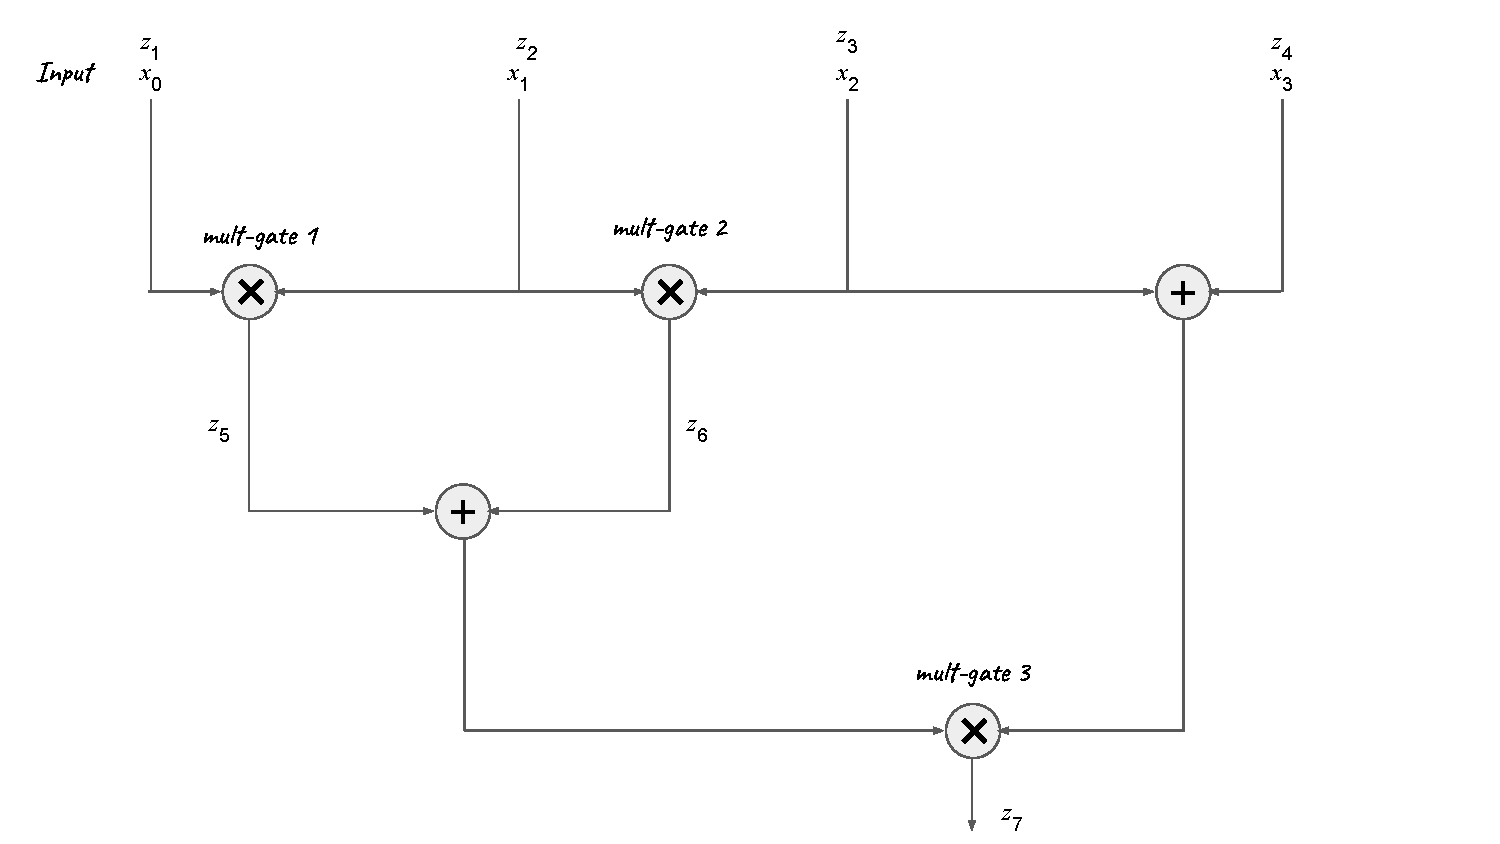
\includegraphics[width=\textwidth]{Figures/Circuit.pdf}
	\caption[An Example of an Arithmetic Circuit]{An example of a Boolean circuit in which \textit{mult-gates} are  \texttt{AND} gates.}
	\label{fig:Arith-circuit}
\end{figure}




\begin{table}[h]
	\centering
\caption[Left and right inputs and output of gates in the example circuit]{Left and right inputs, along with the output of each gate. \texttt{XOR} gates are merged into \texttt{AND} gates.}

	\begin{tabular}{c c c c c c c}
		\toprule
		\textbf{$\text{gate}_i$} & $g_l$& & $g_r$& & $g_o$ &  \\
		\midrule
		1 & $z_1$& $\wedge$ & $z_2$& $\oplus$ & $z_5$ & $= 0$\\

		2 & $z_2$& $\wedge$ & $z_3$& $\oplus$ & $z_6$ & $= 0$\\

		3 & $(z_5 \oplus z_6)$& $\wedge$ & $( z_3 \oplus z_4)$& $\oplus$ & $z_7$ & $= 0$\\
		\bottomrule
	\end{tabular}
	\label{tab:gates}
\end{table}

Accordingly, we can make $\mathbf{A}, \mathbf{B}, \mathbf{C}$ matrices:
\begin{equation}
	\label{eq:ABC-example}
	A = 
	\begin{bmatrix}
		0 & 1 & 0 & 0 & 0 & 0 & 0 & 0\\
		0 & 0 & 1 & 0 & 0 & 0 & 0 & 0\\
		0 & 0 & 0 & 0 & 0 & 1 & 1 & 0
	\end{bmatrix}, B = 
	\begin{bmatrix}
		0 & 0 & 1 & 0 & 0 & 0 & 0 & 0\\
		0 & 0 & 0 & 1 & 0 & 0 & 0 & 0\\
		0 & 0 & 0 & 1 & 1 & 0 & 0 & 0
	\end{bmatrix},
	 C = 
	\begin{bmatrix}
		0 & 0 & 0 & 0 & 0 & 1 & 0 & 0\\
		0 & 0 & 0 & 0 & 0 & 0 & 1 & 0\\
		0 & 0 & 0 & 0 & 0 & 0 & 0 & 1
	\end{bmatrix}
\end{equation}

Consequently, setting $(z_1, z_2, z_3, z_4) = (1, 1, 0, 1)$ (inputs) results the remaining $(z_5, z_6, z_7) = (1, 0, 1)$ which are internal wires or the output. Hence, $\vec{z}^\intercal=(1, 1, 1, 0, 1, 1, 0, 1)$. The computed $\vec{z}$ satisfies $(A\cdot \vec{z})\circ(B\cdot \vec{z})-(C\cdot \vec{z})=0$.

%======================================================================
\chapter{Multiplication of Elements in Binary Extension Field  $\mathbb{F}_{2^{256}}$}\label{a_ch:ff_mult}
%======================================================================

In this appendix we provide the approach existed in~\cite{libff} for multiplying two elements in $a,b \in \mathbb{F}_{2^{256}}$. Let
\begin{equation}\label{eq_F_2_192}
	\mathbb{F}_{2^{256}} := \mathbb{F}_{2}[x]/(x^{256} + x^{10} + x^{5} + x^{2} + 1)
\end{equation}%https://www.jjj.de/mathdata/
	define the field, where $p(x):=x^{256} + x^{10} + x^{5} + x^{2} + 1$ denotes a primitive irreducible polynomial  over $\mathbb{F}_{2}$.  Accordingly, 
	\[
	a(x) \cdot b(x) \bmod p(x)
	\]
	denotes the multiplication of $a$ and $b$ in the field $\mathbb{F}_{2^{256}}$ as defined above, where $a(x)$ and $b(x)$ are the polynomial representations of $a$ and $b$, respectively, as described below.

\paragraph{Partitioning}
Let $a,b \in \mathbb{F}_{2^{256}}$ be represented as  binary polynomials of degree $<256$
\[
	a(x) := a_0 + a_1x + a_2x^2 + a_3x^3 + \dots + a_{255}x^{255} \in \mathbb{F}_{2}[x], 
\]
\[
	b(x) := b_0 + b_1x + b_2x^2 + b_3x^3 + \dots + b_{255}x^{255} \in \mathbb{F}_{2}[x],
\]
such that their polynomial product  $c(x) = a(x) \cdot b(x)$ is represented as
\[
c(x) := c_0 + c_1x + c_2x^2 + c_3x^3 + \dots + c_{510}x^{510} \in \mathbb{F}_{2}[x].
\]
Given a multiplication function $M:\{0,1\}^{64}\times\{0,1\}^{64} \rightarrow \{0,1\}^{128}$ that multiplies two 64-bit binary numbers and is instantiated by the \texttt{CLMUL} instruction on many x86 architecture CPUs~\cite{gueron2010intel}, the Karatsuba multiplication algorithm~\cite{karatsuba1962multiplication} is applied to compute the product of  $a(x)$ and $b(x)$.  To do so, each polynomial is partitioed into four 64-bit limbs \mbox{\(a'_i(x), b'_i(x)\in\{0,1\}^{64}\)} for $i=0,1,2,3$ defined as 
\begin{align*}
	a'_0 (x) &:= a_0 + \dots + a_{63}x^{63}, & 					a'_1 (x) &:= a_{64} +  \dots + a_{127}x^{127}, \\
	a'_2 (x) &:= a_{128} + \dots + a_{191}x^{191}, & 	  a'_3 (x) &:= a_{192} +  \dots + a_{255}x^{255},\\
	b'_0 (x) &:= b_0 + \dots + b_{63}x^{63}, & 				   b'_1 (x) &:= b_{64} +  \dots + b_{127}x^{127}, \\
	b'_2 (x) &:= b_{128} + \dots + b_{191}x^{191}, &	 b'_3 (x) &:= b_{192} +  \dots + b_{255}x^{255}.
\end{align*}
Accordingly, $a $ and $b$ will be represented in terms of $X = x^{64}$ as
\begin{align*}
	a(X)  &= a'_0 + a'_1X + a'_2X^2 + a'_3X^3,\\
	b(X)  &= b'_0 + b'_1X + b'_2X^2 + b'_3X^3.
\end{align*}
Accordingly,  $c$  will be
\begin{align}\label{eq:c_X}
	c(X) := c'_0 + c'_1X + c'_2X^2 +  \dots + c'_{6}X^{6},
\end{align}
where $c'_i \in \{0,1\}^{128}$ for $i=0, \dots, 6$ are overlapping 128-bit limbs in $c(X)$. 

\paragraph{Polynomial Multiplication Algorithm}
Now, we present the multiplication algorithm used in~\cite{libiop}. Given the function $M$ previously defined, let $t$ and $u$, $v$ intermediate auxilary 128-bit binary variables have the following values:
\begin{align*}
	t &:= M(a'_1,b'_1), \\
	u &:= M(a'_2,b'_2), \\
	v &:= t \oplus^{128} u,
\end{align*}
where $\oplus^{128}:\{0,1\}^{128}\times\{0,1\}^{128} \rightarrow \{0,1\}^{128}$ denotes the 128-bit XOR opreator. Moreover, the following values are 64-bit itermediate auxilary variables:
\begin{align*}
	w_0 &:= a'_0 \oplus^{64} a'_1,  &y'_0 &:= b_0 \oplus^{64} b'_1, \\
	w_1 &:= a'_0 \oplus^{64} a'_2,  &y_1 &:= b'_0 \oplus^{64} b'_2, \\
	w_2 &:= a'_2 \oplus^{64} a'_3,  &y_2 &:= b'_2 \oplus^{64} b'_3, \\
	w_3 &:= a'_1 \oplus^{64} a'_3,  &y_3 &:= b'_1 \oplus^{64} b'_3, \\
	w_4 &:= w_0 \oplus^{64} w_2,  &y_4 &:= y_0 \oplus^{64} y_4, \\
\end{align*}
where $\oplus^{64}:\{0,1\}^{64}\times\{0,1\}^{64} \rightarrow \{0,1\}^{64}$ denotes the 64-bit XOR opreator.
Using these, the valuse of $c'_i$s are computed as follows:
 \begin{align*}
 	c'_0 &:= M(a_0,b_0), \\
 	c'_6 &:= M(a_3,b_3), \\
 	c'_1 &:= M(w_0, y_0) \oplus^{128} c'_0 \oplus^{128} t, \\
 	c'_2 &:= M(w_1, y_1) \oplus^{128} c'_0 \oplus^{128} v, \\
 	c'_5 &:= M(w_2, y_2) \oplus^{128} c'_6 \oplus^{128} u, \\
 	c'_4 &:= M(w_3, y_3) \oplus^{128} c'_6 \oplus^{128} v, \\
 	c'_3 &:= M(w_4, y_4) \oplus^{128} c'_0 \oplus^{128} c'_1 \oplus^{128} c'_2 \oplus^{128} c'_4 \oplus^{128} c'_5 \oplus^{128} c'_6. \\
 \end{align*}
 
 Now, the overlapping $c_i$s in (\ref{eq:c_X}) are merged to represent $c(X)$ as non-overlaping  four 128-bit limbs $c''_i \in \{0,1\}^{128}$ for $i=0,\dots,3$, such that
 \begin{align} \label{eq:c_Y}
 c(Y) := c''_0 + c''_1Y + c''_2Y^2 +  c''_{3}Y^{3},
\end{align}
 where $Y = x^{128}$ and each $c''_i$ is computed as follows:
 \begin{align*}
 	c''_0 &:= c'_0   \oplus^{128} (c'_1 \ll 64),\\
 	c''_1 &:= c'_2   \oplus^{128} (c'_1 \gg 64) \oplus^{128} (c'_3 \ll 64),\\
 	c''_2 &:= c'_4   \oplus^{128} (c'_3 \gg 64) \oplus^{128} (c'_5 \ll 64),\\
 	c''_3 &:= c'_6   \oplus^{128} (c'_5 \gg 64),\\
 \end{align*}
 where $\ll 64$ shifts the bits to the left by 64 positions, discarding the bits shifted out from the most significant end and inserting zeros into the least significant positions. Similarly, $\gg 64$ shifts the bits to the right by 64 positions, discarding the bits shifted out from the least significant end and inserting zeros into the most significant positions.
\paragraph{Reduction}
In this step, the polynomial in~(\ref{eq:c_Y}) is reduced modulo \( p(x) \). Then the final result lies in \( \mathbb{F}_{2^{256}} \), and is denoted as
	\[
	d(x) := a(x) \cdot b(x) \bmod p(x),
	\]
where \( d(x) = d_0 + d_1x + \cdots + d_{255}x^{255} \) is the polynomial representation of \( d \in \mathbb{F}_{2^{256}} \), which can alternatively be expressed using four 64-bit limbs as	
\begin{align}
	d(X) := d'_0 + d'_1X + d'_2X^2 + d'_3X^3,
\end{align}
where \( d'_i \in \{0,1\}^{64} \) for \( i = 0,1,2,3 \).
Let us define the polynomial \( p'(x) := x^{10} + x^{5} + x^{2} + 1 \) from $p(x)$, corresponding to the 10-bit binary number \( p' = (10000100101)_2 \).
To compute \( d(X) \), we assume the following partitioning of terms in (\ref{eq:c_Y}) into two 64-bit limbs:
 \begin{align*}
 	c''_0 &:= c''_{00} + c''_{01}X,& c''_1 &:= c''_{10} + c''_{11}X,\\
	c''_2 &:= c''_{20} + c''_{21}X,& c''_3 &:= c''_{30} + c''_{31}X,\\
\end{align*}	
where $c''_{i0}, c''_{i1} \in \{0,1\}^{64}$ for $i=0,1,2,3$. Now, we define the following 128-bit auxilary intermediate values
\begin{align*}
	z_0 &:= M(c''_{31},p), &	z_1 &:= M(c''_{30},p), \\
	z_2 &:= M(c''_{21},p), &	z_3 &:= M(c''_{20} \oplus^{64} z_{01} ,p), \\
\end{align*}
where they are partitioned  into two 64-bit limbs as follows:
 \begin{align*}
	z_0 &:= z_{00} + z_{01}X,& z_1 &:= z_{10} + z_{11}X,\\
	z_2 &:= z_{20} + z_{21}X,& z_3 &:= z_{30} + z_{31}X,\\
\end{align*}	
where $z_{i0}, z_{i1} \in \{0,1\}^{64}$ for $i=0,1,2,3$.
 
 
Now, $d'_0, d'_1, d'_2, d'_3$ are computed as follows:

 \begin{align*}
	d'_0 &:= c''_{00} \oplus^{64} z_{30},\\
	d'_1 &:= c''_{01} \oplus^{64} z_{20} \oplus^{64} z_{31},\\
	d'_2 &:= c''_{10} \oplus^{64} z_{10} \oplus^{64} z_{21},\\
	d'_3 &:= c''_{11} \oplus^{64} z_{00} \oplus^{64} z_{11}.\\
\end{align*}
Consequently, $d(X)$ and then $d=a.b$ are derived.
%======================================================================
\chapter{The Pseudocodes of the Algorithms in the Zupply Framework}\label{a_ch:zupply_algorithms}
%======================================================================

%%%%%%%%%%%%%%%%%%%%%%%%%% Init %%%%%%%%%%%%%%%%%%%%%%%%%%
\begin{algorithm}[h]
	\caption{\textsf{Init} ($\textsc{pp}$, $q_{i_1}$) $\rightarrow$ ($\texttt{tx}_{\textsf{Init}}$, $T_{i_1}$) }\label{alg:Init}
	\begin{algorithmic}[1]
		\State {$\textsc{pp}_\mathsf{sig} \gets \textsc{pp}$}
		\State {$\rho_{i_1} \xleftarrow{R} \{0,1\}^{N_\rho}$}
		% \State {$k \gets \mathcal{H}\big(r|| \big[\mathcal{H}\big(e_I.a_{pk}||\rho \big)\big]_{128} \big)$}
		\State {$(\text{PKsig}_{i_1}, \text{SKsig}_{i_1} ) \gets \mathcal{K}_\mathsf{sig}\big(\textsc{pp}_\mathsf{sig}\big) $}
		\State {$\Tilde{T}_{i_1} \gets \big( 
			q_{i_1}, \text{PKsig}_{i_1}, \rho_{i_1} \big)$}, {$T_{i_1} \gets \big(\Tilde{T}_{i_1}, \text{SKsig}_{i_1}\big)$}
		\State {$\texttt{cm}_{i_1} \gets \mathsf{COMM}_{\rho_{i_1}}(\Tilde{T}_{i_1}) $}
		\State{$(\texttt{rt}^{\text{new}}, \mathsf{ind}_{i_1}, \mathsf{path}_{\mathsf{ind}_{i_1}}) \gets \mathsf{MHT}.\mathsf{Add}(\texttt{cm}_{i_1})$}
		\State {$\texttt{tx}_{\textsf{Init}} \gets \big(\texttt{cm}_{i_1}, \texttt{rt}^{\text{new}}, \mathsf{ind}_{i_1}, \mathsf{path}_{\mathsf{ind}_{i_1}}\big)$}
		
		\State {\Return $\texttt{tx}_{\textsf{Init}}, T_{i_1}$}
	\end{algorithmic}
\end{algorithm}
% ###########################################

%%%%%%%%%%%%%%%%%%%%%%%%%% TRANS %%%%%%%%%%%%%%%%%%%%%%%%%%
\begin{algorithm}[h]
	\caption{\textsf{Trans} $\big($\textsc{pp}$, T_{i_1},  \text{PKsig}_{i_2} \big)$ $\rightarrow$ \big($\texttt{tx}_{\textsf{Trans}}, \Tilde{T}_{i_2}, \texttt{Tag}\big)$}\label{alg:trans}
	\begin{algorithmic}[1]
		\State {$\texttt{cm}_{i_1} \gets \mathsf{COMM}_{\rho_{i_1}}(\Tilde{T}_{i_1}) $}
		\If {$\texttt{cm}_{i_1}\notin \mathbf{C}_\tau$} {}
		\State \Return $\perp$
		\EndIf
		\State $(\mathsf{ind}_{i_1}, \mathsf{path}_{\mathsf{ind}_{i_1}}) \gets \mathsf{MHT}.\mathsf{Search}(\texttt{cm}_{i_1})$
		\State {$\mathsf{pk}_\mathsf{Trans} \gets \textsc{pp}$}
		\State $\texttt{eol}_{i_1} \gets \mathcal{H} \big( \rho_{i_1}\big)$
		\State $q_{i_2} \gets q_{i_1}$
		\State {$\rho_{i_2} \xleftarrow{R} \{0,1\}^{N_\rho}$}
		\State {$\Tilde{T}_{i_2} \gets \big( 
			q_{i_2}, \text{PKsig}_{i_2}, \rho_{i_2} \big)$}
		\State {$\texttt{cm}_{i_2} \gets \mathsf{COMM}_{\rho_{i_2}}(\Tilde{T}_{i_2}) $}
		% \State
		\State $x_\textsf{Trans} \gets \big(\texttt{eol}_{i_1}, \texttt{cm}_{i_2}, \texttt{rt}_\tau \big)$
		\State $w_\textsf{Trans} \gets \big( \Tilde{T}_{i_1}, \Tilde{T}_{i_2}, \mathsf{path}_{\mathsf{ind}_{i_1}}\big)$
		\State $\pi_{\textsf{Trans}} \gets \textsf{Prove}\big(\mathsf{pk}_{\textsf{Trans}}, x_{\textsf{Trans}}, w_{\textsf{Trans}}\big)$
		
		\State{$(\texttt{rt}^{\text{new}}, \mathsf{ind}_{i_2}, \mathsf{path}_{\mathsf{ind}_{i_2}}) \gets \mathsf{MHT}.\mathsf{Add}(\texttt{cm}_{i_2})$}
		\State$\texttt{tx}_{\textsf{Trans}} \gets \big(\pi_{\textsf{Trans}}, x_{\textsf{Trans}}, \texttt{eol}_{i_1}, \texttt{cm}_{i_2}, \texttt{rt}^{\text{new}}, \mathsf{ind}_{i_2}, \mathsf{path}_{\mathsf{ind}_{i_2}} \big)$
		
		\State $\texttt{Tag} \leftarrow \mathcal{S}_\mathsf{sig}(\text{SKsig}_{i_1}, \text{PKsig}_{i_2})$
		\State \Return $\texttt{tx}_{\textsf{Trans}}$, $\Tilde{T}_{i_2}$ , $\texttt{Tag}$
	\end{algorithmic}
\end{algorithm}
% ###########################################

%%%%%%%%%%%%%%%%%%%%%%%%%% Merge %%%%%%%%%%%%%%%%%%%%%%%%%%
\begin{algorithm}
	\caption{\textsf{Merge} $\big($\textsc{pp}$, T_{i_{1,2}},  \text{PKsig}_{i_3} \big)$ $\rightarrow$ \big($\texttt{tx}_{\textsf{Merge}}, \Tilde{T}_{i_3}, \texttt{Tag}_{i_{1,2}}\big)$}\label{alg:merge}
	\begin{algorithmic}[1]
		\State {$\texttt{cm}_{i_1} \gets \mathsf{COMM}_{\rho_{i_1}}(\Tilde{T}_{i_1}) $}, {$\texttt{cm}_{i_2} \gets \mathsf{COMM}_{\rho_{i_2}}(\Tilde{T}_{i_2}) $}
		\If {$\texttt{cm}_{i_1}\notin \mathbf{C}_\tau$ or $\texttt{cm}_{i_2}\notin \mathbf{C}_\tau$} {}
		\State \Return $\perp$
		\EndIf
		\State $(\mathsf{ind}_{i_1}, \mathsf{path}_{\mathsf{ind}_{i_1}}) \gets \mathsf{MHT}.\mathsf{Search}(\texttt{cm}_{i_1})$
		\State $(\mathsf{ind}_{i_2}, \mathsf{path}_{\mathsf{ind}_{i_2}}) \gets \mathsf{MHT}.\mathsf{Search}(\texttt{cm}_{i_2})$
		
		\State {$\mathsf{pk}_\mathsf{Merge} \gets \textsc{pp}$}
		\State {$\texttt{eol}_{i_1} \gets \mathcal{H} \big( \rho_{i_1}\big)$, $\texttt{eol}_{i_2} \gets \mathcal{H} \big( \rho_{i_2}\big)$}
		\State $q_{i_3} \gets q_{i_1} +  q_{i_2}$
		\State {$\rho_{i_3} \xleftarrow{R} \{0,1\}^{N_\rho}$}
		\State {$\Tilde{T}_{i_3} \gets \big( 
			q_{i_3}, \text{PKsig}_{i_3}, \rho_{i_3} \big)$}
		\State {$\texttt{cm}_{i_3} \gets \mathsf{COMM}_{\rho_{i_3}}(\Tilde{T}_{i_3}) $}
		% \State
		\State $x_\textsf{Merge} \gets \big(\texttt{eol}_{i_{1,2}}, \texttt{cm}_{i_3}, \texttt{rt}_\tau \big)$
		\State $w_\textsf{Merge} \gets \big( \Tilde{T}_{i_{1,2}}, \Tilde{T}_{i_3}, \mathsf{path}_{\mathsf{ind}_{i_{1,2}}}\big)$
		\State $\pi_{\textsf{Merge}} \gets \textsf{Prove}\big(\mathsf{pk}_{\textsf{Merge}}, x_{\textsf{Merge}}, w_{\textsf{Merge}}\big)$
		
		\State{$(\texttt{rt}^{\text{new}}, \mathsf{ind}_{i_3}, \mathsf{path}_{\mathsf{ind}_{i_3}}) \gets \mathsf{MHT}.\mathsf{Add}(\texttt{cm}_{i_3})$}
		\State$\texttt{tx}_{\textsf{Merge}} \gets \big(\pi_{\textsf{Merge}}, x_{\textsf{Merge}}, \texttt{eol}_{i_{1,2}}, \texttt{cm}_{i_3}, \texttt{rt}^{\text{new}}, \mathsf{ind}_{i_3}, \mathsf{path}_{\mathsf{ind}_{i_3}} \big)$
		% \State $T^{\text{new}} \gets \big( q^{\text{old}}
		% \text{PK}_{\text{sig}}^{\text{new}}, , \rho^{\text{new}}\big)$
		% \State $\mathcal{C} = \text{Enc} \big(\text{pk}_{\text{enc}}, \{T^{\text{old}}.q, \rho^{\text{new}}\big\}\big)$
		\State $\texttt{Tag}_{i_1} \leftarrow \mathcal{S}_\mathsf{sig}(\text{SKsig}_{i_1}, \text{PKsig}_{i_3})$
		\State $\texttt{Tag}_{i_2} \leftarrow \mathcal{S}_\mathsf{sig}(\text{SKsig}_{i_2}, \text{PKsig}_{i_3})$
		
		\State \Return $\texttt{tx}_{\textsf{Merge}}$, $\Tilde{T}_{i_3}$ , $\texttt{Tag}_{i_{1,2}}$
	\end{algorithmic}
\end{algorithm}

% ###########################################

%%%%%%%%%%%%%%%%%%%%%%%%%% Divide %%%%%%%%%%%%%%%%%%%%%%%%%%
\begin{algorithm}
	\caption{\textsf{Divide} $\big($\textsc{pp}$, T_{i_1},  \text{PKsig}_{i_{2,3}}, q_{i_{2,3}} \big)$ $\rightarrow$ \big($\texttt{tx}_{\textsf{Div}}, \Tilde{T}_{i_{2,3}}, \texttt{Tag}_{i_{2,3}}\big)$}\label{alg:divide}
	\begin{algorithmic}[1]
		\State {$\texttt{cm}_{i_1} \gets \mathsf{COMM}_{\rho_{i_1}}(\Tilde{T}_{i_1}) $}
		\If {$\texttt{cm}_{i_1}\notin \mathbf{C}_\tau$ \textbf{or} $q_{i_{1}} \neq q_{i_{2}} + q_{i_{3}}$} 
		\State \Return $\perp$
		\EndIf
		\State $(\mathsf{ind}_{i_1}, \mathsf{path}_{\mathsf{ind}_{i_1}}) \gets \mathsf{MHT}.\mathsf{Search}(\texttt{cm}_{i_1})$
		\State {$\mathsf{pk}_\mathsf{Div} \gets \textsc{pp}$}
		\State $\texttt{eol}_{i_1} \gets \mathcal{H} \big( \rho_{i_1}\big)$
		% \State Select $q_{i_2}$ and $q_{i_3}$ such that $q_{i_1} = q_{i_2} + q_{i_3}$
		\State {$\rho_{i_2} \xleftarrow{R} \{0,1\}^{N_\rho}$, $\rho_{i_3} \xleftarrow{R} \{0,1\}^{N_\rho}$}
		\State {$\Tilde{T}_{i_2} \gets \big(q_{i_2}, \text{PKsig}_{i_2}, \rho_{i_2} \big)$, $\Tilde{T}_{i_3} \gets \big(q_{i_3}, \text{PKsig}_{i_3}, \rho_{i_3} \big)$}
		\State {$\texttt{cm}_{i_2} \gets \mathsf{COMM}_{\rho_{i_2}}(\Tilde{T}_{i_2}) $, $\texttt{cm}_{i_3} \gets \mathsf{COMM}_{\rho_{i_3}}(\Tilde{T}_{i_3}) $}
		% \State
		\State $x_\textsf{Div} \gets \big(\texttt{eol}_{i_1}, \texttt{cm}_{i_{2,3}}, \texttt{rt}_\tau \big)$
		\State $w_\textsf{Div} \gets \big( \Tilde{T}_{i_1}, \Tilde{T}_{i_{2,3}}, \mathsf{path}_{\mathsf{ind}_{i_1}}\big)$
		\State $\pi_{\textsf{Div}} \gets \textsf{Prove}\big(\mathsf{pk}_{\textsf{Div}}, x_{\textsf{Div}}, w_{\textsf{Div}}\big)$
		
		\State{$(\texttt{rt}_1^{\text{new}}, \mathsf{ind}_{i_2}, \mathsf{path}_{\mathsf{ind}_{i_2}}) \gets \mathsf{MHT}.\mathsf{Add}(\texttt{cm}_{i_2})$}
		\State{$(\texttt{rt}_2^{\text{new}}, \mathsf{ind}_{i_3}, \mathsf{path}_{\mathsf{ind}_{i_3}}) \gets \mathsf{MHT}.\mathsf{Add}(\texttt{cm}_{i_3})$}
		\State$\texttt{tx}_{\textsf{Div}} \gets \big(\pi_{\textsf{Div}}, x_{\textsf{Div}}, \texttt{eol}_{i_1}, \texttt{cm}_{i_{2,3}}, \texttt{rt}_{1,2}^{\text{new}}, \mathsf{ind}_{i_{2,3}}, \mathsf{path}_{\mathsf{ind}_{i_{2,3}}} \big)$
		% \State $T^{\text{new}} \gets \big( q^{\text{old}}
		% \text{PK}_{\text{sig}}^{\text{new}}, , \rho^{\text{new}}\big)$
		% \State $\mathcal{C} = \text{Enc} \big(\text{pk}_{\text{enc}}, \{T^{\text{old}}.q, \rho^{\text{new}}\big\}\big)$
		\State $\texttt{Tag}_2 \leftarrow \mathcal{S}_\mathsf{sig}(\text{SKsig}_{i_1}, \text{PKsig}_{i_2})$
		\State $\texttt{Tag}_3 \leftarrow \mathcal{S}_\mathsf{sig}(\text{SKsig}_{i_1}, \text{PKsig}_{i_3})$
		\State \Return $\texttt{tx}_{\textsf{Div}}$, $\Tilde{T}_{i_{2,3}}$ , $\texttt{Tag}_{i_{2,3}}$
	\end{algorithmic}
\end{algorithm}


% ###########################################

%%%%%%%%%%%%%%%%%%%%%%%%%% VerifyTX %%%%%%%%%%%%%%%%%%%%%%%%%%
\begin{algorithm}
	\caption{\textsf{VerifyTX} $\big($\textsc{pp}$, \texttt{tx}_\mathbbm{x} \big)$ $\rightarrow$ $b \in \{0, 1\}$}\label{alg:VerifyTX}
	\begin{algorithmic}[1]
		\State {$\mathbbm{x}$ $\gets$ type of $\texttt{tx}_\mathbbm{x}$ } \Comment{$\mathbbm{x} \in \{\mathsf{Trans}, \mathsf{Merge}, \mathsf{Div}\}$} 
		\State {$\mathsf{vk}_\mathbbm{x}  \gets \textsc{pp}$}
		\State $(x_\mathbbm{x}, \pi_\mathbbm{x}, \texttt{eol}_1, \texttt{cm}_1, \texttt{rt}_1^{\text{new}}, \mathsf{ind}_{1}, \mathsf{path}_{\mathsf{ind}_{1}}) \gets \texttt{tx}$
		
		\If{$\texttt{eol}_1 \in  \mathbf{X}_\tau$}
		\State \Return 0
		\EndIf
		
		\If{$\mathbbm{x} = \mathsf{Merge}$}
		\State {$\texttt{eol}_2 \gets \texttt{tx}$}
		\If{$\texttt{eol}_2 \in  \mathbf{X}_\tau$}
		\State \Return 0
		\EndIf
		\EndIf
		
		
		\If{$\textsf{Verify}\big(\mathsf{vk}_\mathbbm{x}, x_\mathbbm{x}, \pi_\mathbbm{x} \big) \neq 1$}
		\State \Return 0
		\EndIf
		% \State $() \gets \texttt{tx}$
		\If {$\mathsf{MHT}.\mathsf{Verify}(\texttt{rt}_{\tau}, \texttt{rt}_1^{\text{new}}, \texttt{cm}_1, \mathsf{ind}_1, \mathsf{path}_{\mathsf{ind}_1}) \neq 1$}
		\State \Return 0
		\EndIf
		\If{ $\mathbbm{x} = \mathsf{Div}$} 
		\State $(\texttt{cm}_2, \texttt{rt}_2^{\text{new}}, \mathsf{ind}_{2}, \mathsf{path}_{\mathsf{ind}_{2}}) \gets \texttt{tx}$
		\If {$\mathsf{MHT}.\mathsf{Verify}(\texttt{rt}_1^{\text{new}}, \texttt{rt}_2^{\text{new}}, \texttt{cm}_2, \mathsf{ind}_2, \mathsf{path}_{\mathsf{ind}_2}) \neq 1$}
		\State \Return 0
		\EndIf
		
		\EndIf
		
		% \If{$\textsf{Verify}()$}
		\State \Return 1
	\end{algorithmic}
\end{algorithm}


% ###########################################


%%%%%%%%%%%%%%%%%%%%%%%%%% Upload %%%%%%%%%%%%%%%%%%%%%%%%%%
\begin{algorithm}
	\caption{\textsf{Upload} $\big($\textsc{pp}$, [\textsf{pred}], T_i, d_{\mathsf{pub}}, d_{\mathsf{pri}}, \textsc{k}_{n_3}, [\textsf{tags}]  \big)$ $\rightarrow$ $d_{n_3}$}\label{alg:Upload}
	\begin{algorithmic}[1]
		\State {$\mathsf{pk}_\mathsf{Auth} \gets \textsc{pp}$}
		\State {$\texttt{cm}_{i_1} \gets \mathsf{COMM}_{\rho_{i_1}}(\Tilde{T}_{i_1}) $}
		\State $(\mathsf{ind}_{i_1}, \mathsf{path}_{\mathsf{ind}_{i_1}}) \gets \mathsf{MHT}.\mathsf{Search}(\texttt{cm}_{i_1})$
		\State $(\text{PKsig}_{i}, \text{SKsig}_{i}) \gets T_i$
		\State $c_{n_3} \gets \mathcal{E}_\mathsf{sym}(\textsc{k}_{n_3}, d_{{n_3}, \mathsf{pri}} )$
		\State $x_\texttt{Auth} \gets (\texttt{rt}_\tau, \text{PKsig}_{i})$
		\State $w_\texttt{Auth} \gets (T_i, \mathsf{path}_{\mathsf{ind}_{i}})$
		\State $\pi_{\textsf{Auth}} \gets \textsf{Prove}\big(\mathsf{pk}_{\textsf{Auth}}, x_{\textsf{Auth}}, w_{\textsf{Auth}}\big)$
		\State $m \gets ([\textsf{pred}], d_{\mathsf{pub}}, c_{n_3}, [\textsf{tags}], \pi_{\textsf{Auth}}, x_\texttt{Auth}, \mathbf{L}_\tau^\mathsf{PI}(\texttt{rt}_\tau))$
		\State $\sigma_{n_3} \gets \mathcal{S}_\mathsf{sig}\big(\text{SKsig}_{i}, m \big)$
		\State $d_{n_3} \gets \big([\textsf{pred}],  d_{\mathsf{pub}}, c_{n_3},
		[\textsf{tags}], \pi_\texttt{Auth}, x_\texttt{Auth}, \mathbf{L}_\tau^\mathsf{PI}(\texttt{rt}_\tau), \sigma_{n_3}\big)$
		\State \Return $d_{n_3}$
	\end{algorithmic}
\end{algorithm}


% ###########################################

%%%%%%%%%%%%%%%%%%%%%%%%%% Audit %%%%%%%%%%%%%%%%%%%%%%%%%%
\begin{algorithm}
	\caption{\textsf{Audit} $\big($\textsc{pp}$, d_n  \big)$ $\rightarrow$ $b \in \{0, 1\}$}\label{alg:Audit}
	\begin{algorithmic}[1]
		\State {$\mathsf{vk}_\mathsf{Auth} \gets \textsc{pp}$}
		\State {$\big([\textsf{pred}],  d_{\mathsf{pub}}, c_{n},
			[\textsf{tags}], \pi_\texttt{Auth}, x_\texttt{Auth}, \mathbf{L}_\tau^\mathsf{PI}(\texttt{rt}_\tau), \sigma_{n}\big) \gets d_{n}$}
		\State $(\texttt{rt}_\tau, \text{PKsig}_{i}) \gets x_\texttt{Auth}$
		\State $m \gets ([\textsf{pred}], d_{\mathsf{pub}}, c_{n}, [\textsf{tags}], \pi_{\textsf{Auth}}, x_\texttt{Auth})$
		
		\If{$\mathbf{L}_\tau^\mathsf{PI}(\texttt{rt}_\tau)$ is not valid}
		\State \Return 0
		\EndIf
		
		\If{$\mathcal{V}_\mathsf{sig}(\text{PKsig}_{i}, m, \sigma_{n}) = 0$}
		\State \Return 0
		\EndIf
		
		\If{$\mathsf{Verify}(\mathsf{vk}_\mathsf{Auth}, x_\texttt{Auth}, \pi_\texttt{Auth}) = 0$}
		\State \Return 0
		\EndIf
		
		\While {\textbf{not} $\textsf{pred}.\textsf{isEmpty}()$ } 
		\State {$\textsc{cid} \gets \mathsf{pred}.\mathsf{pop}()$}
		\State $d_p \gets \mathsf{DCS}(\textsc{cid})$
		\State $\text{PKsig}_{j} \gets d_p$
		\If{$\text{PKsig}_{i} \neq \text{PKsig}_{j}$}
		\State {$\texttt{Tag} \gets \mathsf{tags}.\mathsf{pop}()$}
		\If{$\mathcal{V}_\mathsf{sig}(\text{PKsig}_{j}, \text{PKsig}_{i}, \texttt{Tag}) = 0$}
		\State \Return 0
		\EndIf
		\EndIf
		\EndWhile
		\State \Return 1
	\end{algorithmic}
\end{algorithm}

% ###########################################


% GLOSSARIES (Lists of definitions, abbreviations, symbols, etc. provided by the glossaries-extra package)
% -----------------------------
\printglossary
\cleardoublepage
\phantomsection		% allows hyperref to link to the correct page

%----------------------------------------------------------------------
\end{document} % end of logical document
